%%%%%%%%%%%%%%%%%%%%%%%%%%%%%%%%%%%%%%%%%
% Conference Booklet
% LaTeX Template
% Version 1.0 (22/12/2019)
%
% This template originates from:
% https://www.LaTeXTemplates.com
%
% Authors:
% Maxime Lucas (ml.maximelucas@gmail.com) 
% Pau Clusella
% Modifications for LaTeX Templates by Vel (vel@LaTeXTemplates.com)
%
% License:
% GNU General Public License v3.0
%
%%%%%%%%%%%%%%%%%%%%%%%%%%%%%%%%%%%%%%%%%

%----------------------------------------------------------------------------------------
%	PACKAGES AND OTHER DOCUMENT CONFIGURATIONS
%----------------------------------------------------------------------------------------

\documentclass[
	openany, % Allow chapters to start on odd and even pages
	parskip=full, % Large space between paragraphs
	12pt, % Default font size
	a4paper, % Paper size, use letterpaper for US letter size
]{conferencebooklet} % Custom class defining the style and layout of the template

%----------------------------------------------------------------------------------------

%\usepackage[utf8]{inputenc}
%\usepackage[T1, T2A]{fontenc}
\usepackage{enumitem}
\usepackage{scalerel}
\usepackage{multirow}
\usepackage{xcolor}
\usepackage{nicematrix}
\usepackage{amssymb}
\usepackage{xtab}
\usepackage{tabularray, ragged2e}
% \DefTblrTemplate{caption}{default}{}
% \SetTblrInner[tblr,longtblr]{rowsep=0pt}
% \RenewDocumentCommand\TblrAlignLeft{}{\RaggedRight}

\newcommand{\ab}[1]{\textcolor{blue}{#1}}
\newcommand\smallbull{\scaleobj{0.7}{\blacksquare}}
\newcommand\itema{\item[\textcolor{case_blue}{$\smallbull$}]}

\definecolor{case_blue}{RGB}{0, 120, 174}

\begin{document}

%----------------------------------------------------------------------------------------
%	 COVER PAGE
%----------------------------------------------------------------------------------------

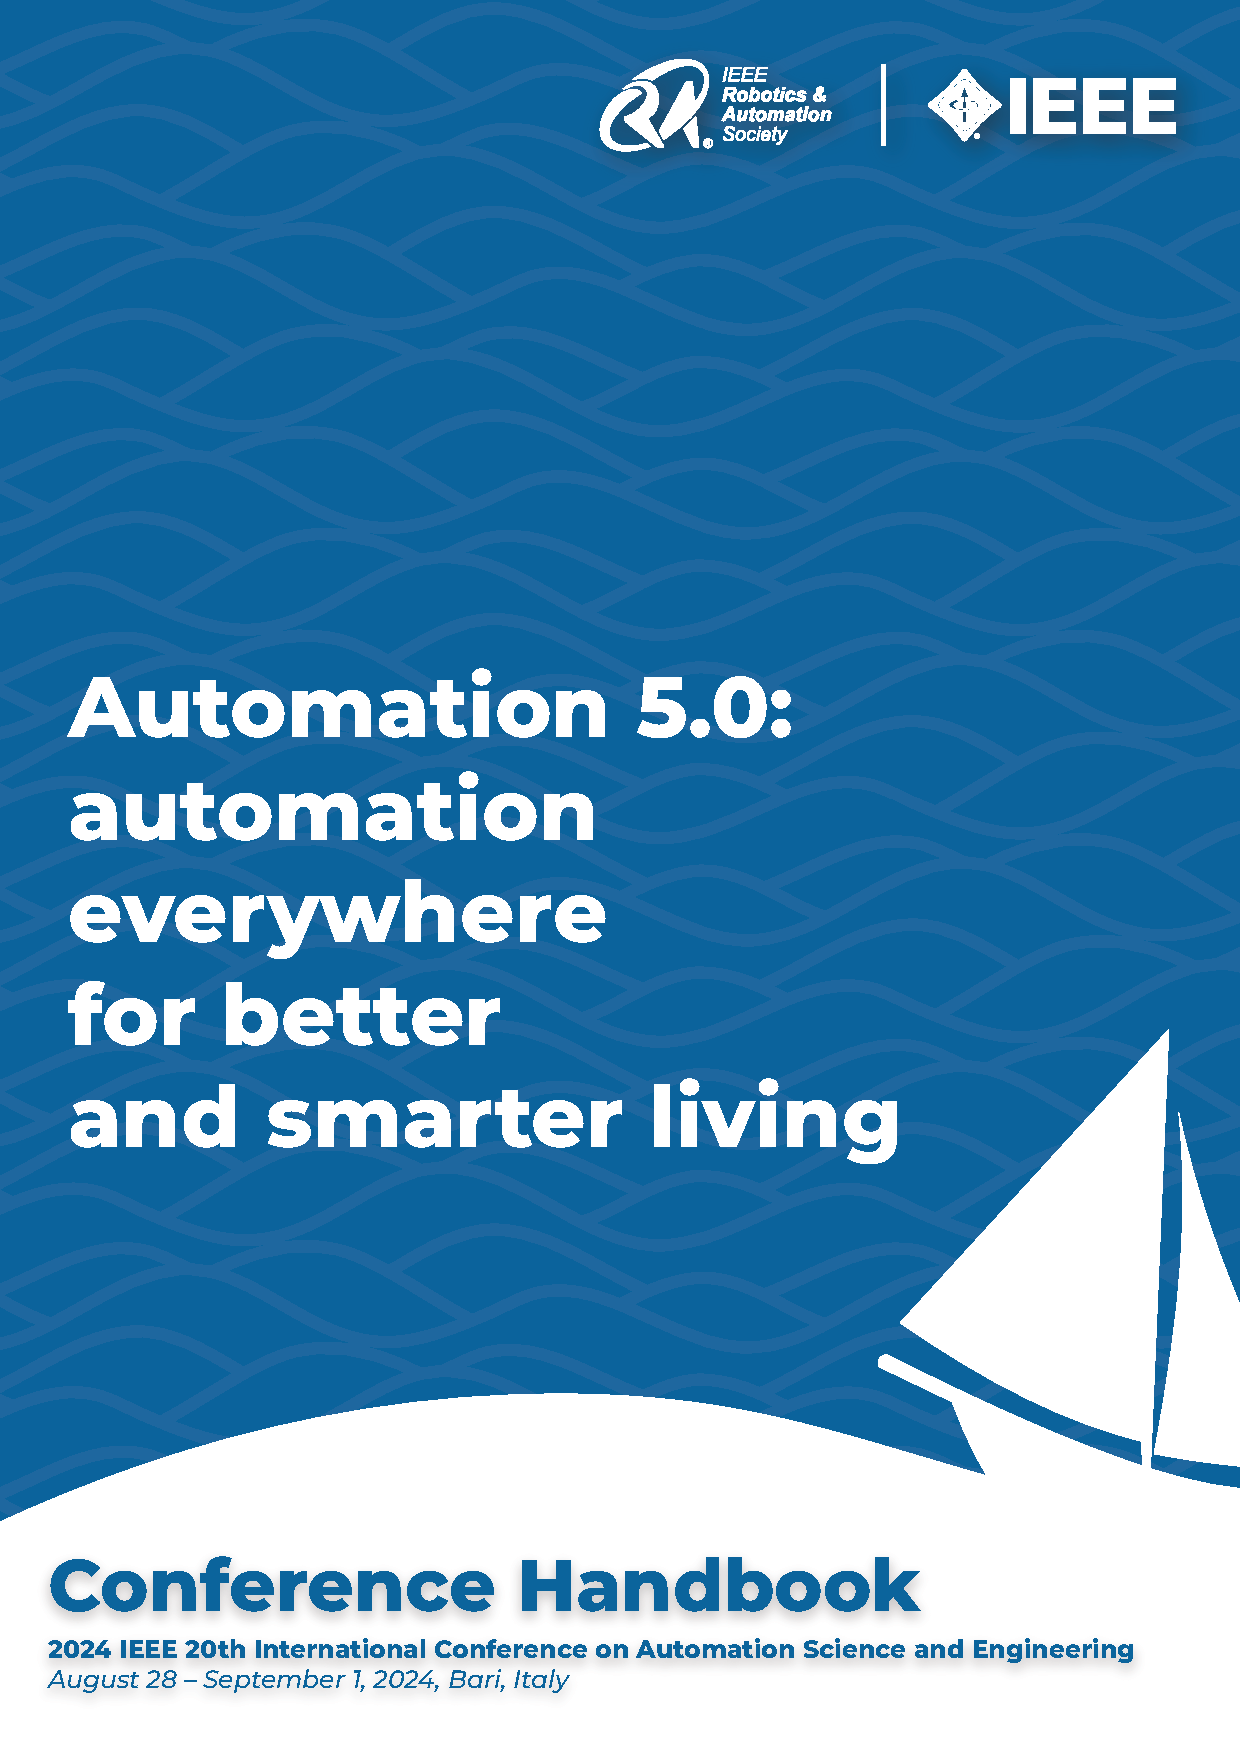
\includepdf{images/Frontpage.pdf} % The cover for the booklet is included as a whole-page image, it can be a PDF or an image file but must be the same dimensions as the paper size

\newpage


%----------------------------------------------------------------------------------------
%	 INFORMATION/COPYRIGHT PAGE
%----------------------------------------------------------------------------------------

\thispagestyle{empty} % Suppress headers and footers on this page

~\vfill % Push text down

\begin{center}
    \begin{tabular}{cc}
    	
\includegraphics[width=0.2\textwidth]{images/qr/case.pdf} \hspace{20mm} & 
\includegraphics[width=0.2\textwidth]{images/qr/infovaya.pdf}
    \end{tabular}
\end{center}

\begin{center}	
    The source code for this handbook can be found at \url{https://github.com/nicomignoni/case24-booklet}. \\ This template originates from \url{LaTeXTemplates.com} and is based on the one at  \url{https://github.com/maximelucas/AMCOS\_booklet}
\end{center}

\newpage
\thispagestyle{empty} % Suppress headers and footers on this page
~

\newpage
\thispagestyle{empty} % Suppress headers and footers on this page
~

\newpage

\newpage


%----------------------------------------------------------------------------------------
%	 TABLE OF CONTENTS
%----------------------------------------------------------------------------------------

\tableofcontents

\newpage
\thispagestyle{empty} % Suppress headers and footers on this page
~

%----------------------------------------------------------------------------------------
%	 ABOUT CONFERENCE
%----------------------------------------------------------------------------------------
\chapter{Welcome Message}
On behalf of the Organizing Committee, it is our great pleasure to extend a warm welcome to all participants attending the \textit{IEEE 20th International Conference on Automation Science and Engineering (CASE 2024)}, taking place in charming Puglia, Italy, from August 28 – September 1, 2024. As one of the flagship conferences of the IEEE Robotics \& Automation Society, CASE is a prestigious international platform for researchers and practitioners to present and discuss their cutting-edge work in the automation field. We are delighted to host this significant event in Puglia, an idyllic, sun-kissed region on the Adriatic Sea coast, known for its rich history, vibrant culture, and warm hospitality.

CASE 2024 brings together various activities, including plenary and keynote sessions, contributed paper sessions, workshops, engaging industry panel discussions, and several social events. The conference will focus on the theme "Automation 5.0: Automation Everywhere for Better and Smarter Living" and will cover a wide range of topics such as Systems, Automation, Control Theory, Autonomous Systems, Discrete Event Systems, Smart Cities, Robotics, Building Automation, Smart Mobility, Information and Communication Technologies, and Factory 4.0.

This year marks a milestone in CASE's history as we celebrate the 20th anniversary of this conference. Since its first edition in 2005 in Edmonton, Alberta, Canada, CASE has become a cornerstone event in the automation community, fostering innovation, collaboration, and knowledge exchange. We invite you to commemorate this special anniversary with celebratory activities.

CASE 2024 is already a resounding success, drawing more than 900 participants from around the globe and more than 20 industrial, scientific, and institutional sponsors, making this conference an outstanding event. We received an overwhelming number of submissions from more than 50 countries. The conference saw a 28\% increase in regular paper submissions and a 67\% increase in special session paper submissions compared to last year. The conference received 44 special session proposals, marking a 29\% increase from the previous year. In total, 721 regular and special session papers were submitted, of which 544 were accepted. Additionally, we received 133 presentation-only papers, including 48 RAL/T-ASE/T-RO papers. Lastly, CASE 2024 received 17 workshop proposals of extremely high quality.

This year, we introduced a Call for Application Video for the first time, receiving more than 80 submissions. In line with our commitment to diversity and inclusion, CASE 2024 also featured a new Call for Diversity and Inclusion Activities, encouraging proposals that broaden participation in automation science and engineering and encompass various dimensions of diversity.

Besides the traditional awards such as the \textit{Best Conference Paper Award},\textit{Best Application Paper Award}, \textit{Best Student Paper Award}, and the Best Healthcare Automation Paper Award, we are proud to present for the second time the \textit{Peter Luh Memorial Best Paper Award for Young Researcher}, which has now become an official IEEE award. This award was established in honor of Professor Peter Luh's dedicated service to raising the profile of automation and supporting young researchers early in their careers. This year, the conference also established the \textit{Best Short Paper Award} and the \textit{Best Application Video Award}. This year the \textit{IEEE T-ASE Best Paper Award} and \textit{IEEE T-ASE Best Application Paper Award} will be presented at CASE.



Several opportunities were available this year to participants. RAS established the traditional Travel Support, Social Media Ambassador, and IDEA Travel Support. This year, we introduced several new opportunities. We sent out a call for Student Volunteers, providing 15 students from all around the globe with the opportunity to participate in the conference for free. 
Furthermore, we are thrilled to introduce the RAS Member Support Program (MSP) for CASE for the first time. This program aims to provide financial support to members who contribute to activities aligned with the RAS mission. The MSP offers a significant discount on registration fees. Additionally, we are pleased to offer onsite childcare support to facilitate parents' participation, with discounted options for IEEE RAS members.

We extend our heartfelt gratitude to the Authors, Reviewers, Conference Editorial Board, Steering Committee, Organizing Committee, and volunteers whose dedication and hard work have made CASE 2024 possible. 

Thank you for joining us in Bari for CASE2024. We look forward to a vibrant and enriching conference experience and to seeing the innovative contributions that will shape the future of automation.

\textit{On behalf of the Organising Committee of IEEE CASE 2024}


\begin{tabular}{wc{50mm}wc{50mm}wc{50mm}}
    \multicolumn{1}{c}{\includegraphics[width=0.2\textwidth]{images/people/dotoli-circle.png}} & 
    \multicolumn{1}{c}{\includegraphics[width=0.2\textwidth]{images/people/sun-circle.png}} & 
    \multicolumn{1}{c}{\includegraphics[width=0.2\textwidth]{images/people/seatzu-circle.png}} \\
    Mariagrazia DOTOLI & Yu SUN & Carla SEATZU \\
    \textit{General Chair} & \textit{General Co-Chair} & \textit{Program Chair}
\end{tabular}





\chapter{About}
The 2024 IEEE 20th International Conference on Automation Science and Engineering (CASE 2024) is one of the three flagship conferences of the IEEE Robotics \& Automation Society and provides a primary forum for cross-industry multidisciplinary research in automation.

CASE 2024 will be held on August 28 – September 1, 2024, in charming Puglia (or Apulia), Italy. Puglia is a little slice of idyllic, sun-kissed Italia on the Adriatic Sea coast. An important economic center in Southern Italy, it is also a bridge between West and East with a multicultural, open, and friendly community.

The conference will focus on Automation 5.0: automation everywhere for better and smarter living and will include tutorials and workshops, a technical program of presentations, keynote lectures, and social events. The conference will cover a wide range of topics on Systems, Automation, Control theory, Autonomous Systems, Discrete Event Systems, Smart Cities, Robotics, Building Automation, Smart Mobility, Information and Communication Technologies, and Factory 4.0.

\section{History of CASE: Celebrating 20 Years of Innovation and Progress in Automation}
The Conference on Automation Science and Engineering (CASE) is an influential annual event organized by the IEEE Robotics and Automation Society. Since its establishment in Edmonton 2005, CASE has provided a dedicated platform for researchers, academics, and industry professionals to share and discuss advances in automation science and engineering. This initiative arose from the recognition of the increasing importance of automation in various industrial and research domains. In its early years, CASE focused on foundational topics such as control systems, robotics, discrete event systems, and manufacturing automation. The conference aimed to bridge the gap between theoretical advancements and practical applications, fostering interdisciplinary collaboration and innovation. This approach quickly garnered attention and the conference grew in prominence, attracting a global audience eager to explore the latest developments in automation.

Between 2011 and 2015, CASE broadened its thematic scope to include emerging areas such as biomedical and sustainable automation, service robotics, and smart systems. This period marked the conference’s expansion in terms of both subject and geographic reach. By rotating its location globally between America, Asia, and Europe, CASE reflected its international significance and fostered greater diversity in participation. Additionally, the conference placed a stronger emphasis on workshops, special sessions, and industry panels, enhancing opportunities for networking and collaborative research. This focus on interaction and practical application helped solidify CASE’s reputation as a premier event in the field.

From 2016 to the present, CASE has embraced and integrated advancements in artificial intelligence, machine learning, and the Internet of Things (IoT) into the realm of automation science and engineering. The conference has continued to promote interdisciplinary research, addressing complex challenges in various sectors such as healthcare, transportation, and energy. This era also saw CASE adapting to global circumstances, particularly the COVID-19 pandemic, by adopting virtual and hybrid formats. These adaptations ensured that the conference could continue its mission of knowledge sharing and engagement despite the challenges posed by the pandemic. Recent conferences have also placed a spotlight on sustainability and ethical considerations in automation, reflecting broader societal concerns and the need for responsible innovation.

Throughout its history, CASE has significantly contributed to the body of knowledge in automation science and engineering. By publishing high-quality research and fostering a culture of innovation, CASE has built a strong community of professionals dedicated to advancing automation technologies and their applications. The conference has not only kept pace with technological advancements but has also anticipated and shaped future trends in the field. As it continues to evolve, CASE addresses new challenges and opportunities in automation, maintaining its relevance and leadership.

Overall, CASE has grown from a niche event to a key global forum that shapes the future of automation. Its comprehensive and inclusive approach has ensured that it remains at the forefront of the field, driving progress and fostering a collaborative international community. The conference’s legacy of promoting interdisciplinary research, practical innovation, and ethical considerations continues to influence the direction of automation science and engineering worldwide.

Since CASE 2024 is the 20th CASE conference, this anniversary will be celebrated at the conference through different events, including videos and presentations. We will hear how CASE was initiated and get short memories from the former conferences in Edmonton 2005, Shanghai 2006, Scottsdale 2007, Arlington 2008, Bangalore 2009, Toronto 2010, Trieste 2011, Seoul 2012, Madison 2013, Taipei 2014, Gothenburg 2015, Fort Worth 2016, Xi’an 2017, Munich 2018, Vancouver 2019, Hong Kong 2020, Lyon 2021, Mexico City 2022, and Auckland 2023. Some statistics will also confirm the conference's growth, for instance, the increase by a factor of seven in the number of papers from the first CASE conference to this year’s CASE in Bari.

% \begin{figure}
%     \centering
%     \includegraphics[width=\linewidth]{images/map.png}
%     % \caption{Enter Caption}
% \end{figure}

\newpage

\section{Organizing committee}
\begin{table}[h!]
    \subfloat{
        \begin{tabular}{p{75mm}}
            \large \textbf{General Chair} \\
            \textbf{Mariagrazia DOTOLI} \\
            \textit{Polytechnic of Bari} \\ \\
            \large \textbf{General Co-Chair} \\
            \textbf{Yu SUN} \\
            \textit{University of Toronto} \\ \\
            \large \textbf{Program Chair} \\
            \textbf{Carla SEATZU} \\ 
            \textit{University of Cagliari}  \\ \\
            \large \textbf{Program Committee Co-Chairs} \\
            \textbf{Dimos DIMAROGONAS} \\
            \textit{KTH Royal Institute of Technology} \vspace{2mm} \\
            \textbf{Bengt LENNARTSON} \\
            \textit{Chalmers University of Technology} \vspace{2mm} \\
            \textbf{Spyros REVELIOTIS} \\
            \textit{Georgia Institute of Technology} \vspace{2mm} \\ 
            \textbf{Michael Yu WANG} \\ 
            \textit{Great Bay University} \vspace{2mm} \\
            \textbf{Qianchuan ZHAO} \\
            \textit{Tsinghua University} \vspace{2mm} \\ \\
            \large \textbf{Publicity Chairs} \\
            \textbf{Tiantian XU} \\
            \textit{Shenzhen Institutes of Advanced Technology, CAS} \vspace{2mm} \\ 
            \textbf{Jingang YI} \\
            \textit{Rutgers University} \vspace{2mm} \\ \\
            \large \textbf{Conference Treasurer} \\
            \textbf{Raffaele CARLI} \\
            \textit{Polytechnic of Bari} \\ \\
            \large \textbf{Publication Chair} \\
            \textbf{Mauro FRANCESCHELLI} \\ 
            \textit{University of Cagliari} \\ \\
            \large \textbf{Publication Co-Chair} \\
            \textbf{Emmanuel DEAN} \\ 
            \textit{Chalmers University}
        \end{tabular}
    } \hspace{10mm}
    \subfloat{
        \begin{tabular}{p{75mm}}
            \large \textbf{Special Session Chairs} \\
            \textbf{Kai CAI} \\
            \textit{Osaka Metropolitan University} \\ 
            \textbf{Raffaele CARLI} \\
            \textit{Polytechnic of Bari} \vspace{2mm} \\
            \textbf{Claudio SAVAGLIO} \\
            \textit{University of Calabria} \vspace{2mm} \\
            \textbf{Ying (Gina) TANG} \\ 
            \textit{Rowan University} \vspace{2mm} \\
            \textbf{Mengchu ZHOU} \\
            \textit{New Jersey Institute of Technology}\vspace{2mm} \\ \\
            \large \textbf{Workshop \& Tutorial Chairs} \\
            \textbf{Maria Pia FANTI} \\
            \textit{Polytechnic of Bari} \vspace{2mm} \\
            \textbf{Christoforos HADJICOSTIS} \\
            \textit{University of Cyprus} \vspace{2mm} \\
            \textbf{Chiwoo PARK} \\
            \textit{KTH Royal Institute of Technology} \vspace{2mm} \\
            \textbf{Xinyu WU} \\ 
            \textit{Shenzhen Institutes of Advanced Technology} \\ \\
            \large \textbf{Industrial \& Exhibition Chair} \\
            \textbf{Birgit VOGEL-HEUSER} \\ 
            \textit{Technical University of Munich} \\ \\
            \large \textbf{Exhibition \& Sponsorship Chair} \\
            \textbf{Kazuhiro SAITOU} \\ 
            \textit{University of Michigan} \\ \\
            \large \textbf{Local Arrangement Chair} \\
            \textbf{Paolo SCARABAGGIO} \\
            \textit{Polytechnic of Bari} \vspace{2mm} \\ \\
            \large \textbf{Local Arrangement Co-Chairs} \\
            \textbf{Graziana CAVONE} \\
            \textit{University of Rome 3} \vspace{2mm} \\
            \textbf{Nicola EPICOCO} \\
            \textit{Libera Università Mediterranea} \vspace{8 mm}
        \end{tabular}
    }
\end{table}

\begin{table}[h!]
    \subfloat{
        \begin{tabular}{p{75mm}}
            \large \textbf{Diversity \& Inclusion Committee Chairs} \\
            \textbf{Graziana CAVONE} \\
            \textit{University of Rome 3} \vspace{2mm} \\
            \textbf{Hyun-Jung KIM} \\
            \textit{KAIST} \\ \\ 
            \large \textbf{Website Committee Chair} \\
            \textbf{Paolo SCARABAGGIO} \\
            \textit{Polytechnic of Bari}
        \end{tabular}
    } \hspace{10mm}
    \subfloat{
        \begin{tabular}{p{75mm}}
            \large \textbf{Award Committee Chair} \\
            \textbf{Michael Yu WANG} \\
            \textit{Great Bay University} \\ \\
            \large \textbf{Student Activity Chair} \\
            \textbf{Nicola MIGNONI} \\ 
            \textit{Polytechnic of Bari} \vspace{1.5mm}
        \end{tabular}
    }
\end{table}
\vfill

\section{Steering committee}

\begin{table}[h!]
    \subfloat{
        \begin{tabular}{p{75mm}}
            \textbf{Fan-Tien CHENG} (Chair) \\  
            \textit{Nat. Cheng Kung University}  \vspace{2mm} \\
            \textbf{Nak Young CHONG}  \\
            \textit{Japan Advanced Inst. of Sci. and Tech.} \vspace{2mm} \\
            \textbf{Stéphane DAUZÈRE-PÉRÈS} \\
            \textit{MINES Saint-Etienne} \vspace{2mm}  \\    
            \textbf{Mariagrazia DOTOLI}  \\
            \textit{Politecnico di Bari} \vspace{2mm} \\
            \textbf{Martin FABIAN} \\
            \textit{Chalmers University of Tech. } \vspace{2mm} \\
            \textbf{Maria Pia FANTI} \\
            \textit{Politecnico di Bari} \vspace{2mm} \\
            \textbf{Cesare FANTUZZI} \\
            \textit{University of Modena \& Reggio Emilia} \vspace{2mm} \\ 
            \textbf{Ken GOLDBERG} \\
            \textit{UC Berkeley} \vspace{2mm} \\                  
            \textbf{Xiaohong GUAN} \\
            \textit{Xian Jiaotong University} \vspace{2mm} \\ 
            \textbf{George Q. HUANG} \\
            \textit{University of Hong Kong} \vspace{2mm} \\ 
            \textbf{Qing-Shan JIA} \\
            \textit{Tsinghua University} \vspace{2mm} \\ 
            \textbf{Bengt LENNARTSSON} \\
            \textit{Chalmers University of Tech.} \vspace{2mm} \\ 
            \textbf{Jingshan LI} \\
            \textit{University of Wisconsin-Madison} \vspace{2mm} \\
            \textbf{Xiaoou LI} \\
            \textit{National Polytechnic Institute of Mexico} \\
         \end{tabular}
    }
    \subfloat{
        \begin{tabular}{p{75mm}}
            \textcolor{darkgray}{\textbf{Peter B. LUH} (\textit{in memoriam})} \\
            \textcolor{darkgray}{\textit{University of Connecticut}} \vspace{2mm} \\ 
            \textbf{Dan O. POPA } \\
            \textit{University of Louisville} \vspace{2mm} \\ 
            \textbf{Spyros REVELIOTIS} \\
            \textit{Georgia Tech} \vspace{2mm} \\ 
            \textbf{Kazuhiro SAITOU} \\
            \textit{University of Michigan} \vspace{2mm} \\ 
            \textbf{Weiming SHEN} \\
            \textit{Western University} \vspace{2mm} \\ 
            \textbf{Leyuan SHI} \\
            \textit{University of Wisconsin – Madison} \vspace{2mm} \\ 
            \textbf{Yu SUN} \\
            \textit{University of Toronto} \vspace{2mm} \\ 
            \textbf{Birgit VOGEL-HEUSER} \\
            \textit{Technical University Munich} \vspace{2mm} \\ 
            \textbf{Michael WANG} \\
            \textit{Hong Kong University of Sci \&. Tech.} \vspace{2mm} \\ 
            \textbf{Xiaolan XIE} \\
            \textit{MINES Saint-Etienne} \vspace{2mm} \\ 
            \textbf{Xun XU} \\
            \textit{University of Auckland} \vspace{2mm} \\ 
            \textbf{Jingang YI} \\
            \textit{Rutgers University} \vspace{2mm} \\ 
            \textbf{Mengchu ZHOU} \\
            \textit{New Jersey Inst. Tech.} \vspace{2mm} \\ 
            \\
            \\ 
        \end{tabular}
    }
\end{table}

\vfill\null

\section{Editorial Board}

\large \textbf{Editor-in-Chief} \normalsize
\begin{table}[h!]
    \begin{tabular}{l}
        Jingang	Yi 
    \end{tabular}
\end{table}


\large \textbf{Editors} \normalsize
\begin{table}[h!]
    \begin{tabular}{p{42mm}p{46mm}p{32mm}l}
         Houshang	Darabi	&
         Carla	Seatzu	\\
         Qiang	Huang  &	
         Weihua	Sheng	\\
         Qing-Shan	Jia	&
         Ying	Tang \\
         Xinyu	Liu	 &
         Chao-Bo	Yan	
    \end{tabular}
\end{table}

\large \textbf{Associate Editors} \normalsize
\begin{table}[h!]
    \begin{tabular}{llll}
             Knut	Akesson	&
             Zhigang	Jiang	&
             Agostino M. Mangini	&
             Weitian	Wang	\\
             Mohammad	Al Janaideh	&
             Tongdan	Jin	&
             Lars	Moench	&
             Yebin	Wang	\\
             Vincent	Augusto	&
             Feng	Ju	&
             Umberto	Montanaro	&
             Yongjing	Wang	\\
             Ashis	Banerjee	&
             Hyun-Jung	Kim	&
             James	Morrison	&
             Xiaochen	Xian	\\
             Pavel	Burget	&
             He	Kong	&
             Tatsushi	Nishi	&
             Xiaolei	Xie	\\
             Zhengcai	Cao	&
             Nan	Kong	&
             Peng	Pan	&
             Pengwen	Xiong	\\
             Raffaele	Carli	&
             Ilya	Kovalenko	&
             Santiago	Paternain	&
             Qingsong	Xu	\\
             Stefano	Carpin	&
             Guillaume J.	Laurent	&
             Sujit	PB	&
             Bing	Yan	\\
             Graziana	Cavone	&
             Hyo Kyung	Lee	&
             Giulia	Pedrielli	&
             Fajun	Yang	\\
             Abdallah	Chehade	&
             Jun-Ho	Lee	&
             Zhi	Pei	&
             Hui	Yang	\\
             Heping	Chen	&
             Sujee	Lee	&
             Tao	Peng	&
             Liangjing	Yang	\\
             Kuo	Chen	&
             Congbo	Li	&
             Yan	Qiao	&
             Esen	Yel	\\
             Nan	Chen	&
             Gaofeng	Li	&
             Juntian	Qu	&
             Dan	You	\\
             Sandeep	Chinchali	&
             Lefei	Li	&
             Ning	Ran	&
             Claude	Yugma	\\
             Changsheng	Dai	&
             Te	Li	&
             Michele	Roccotelli	&
             Liang	Zhang	\\
             Diego	Deplano	&
             Chao	Liu	&
             Paolo	Scarabaggio	&
             Meng	Zhang	\\
             Dongping	Du	&
             Gaiyun	Liu	&
             Tony	Shi	&
             Xi	Zhang	\\
             Anqing	Duan	&
             Jian	Liu	&
             Rong	Su	&
             Zhi-Hai	Zhang	\\
             Gregory	Faraut	&
             Jun	Liu	&
             U-Xuan	Tan	&
             Lei	Zhao	\\
             Irene	Fassi	&
             Xingjian	Liu	&
             Andrea	Testa	&
             Pai	Zheng	\\
             Gerardo	Flores	&
             Yuanchang	Liu	&
             Yin	Tong	&
             Xiang	Zhong	\\
             Mauro	Franceschelli	&
             Haojian	Lu	&
             Valeria	Villani	&
             Kunpeng	Zhu	\\
             Xiwang	Guo	&
             Yuqian	Lu	&
             Holger	Voos	&
             Qinghua	Zhu	\\
             Yassine	Haddab	&
             Ziyue	Ma	&
             Di	Wang	&
	      	\\
             Min-Hsiung	Hung	&
             Cristian	Mahulea	&
             Gongming	Wang	&
           	\\
   \end{tabular}
\end{table}


\newpage
%----------------------------------------------------------------------------------------
%	 PARTNERS & SPONSORS
%----------------------------------------------------------------------------------------

\chapter{Partner Institutions and Sponsors}



\def\sponsorscaling{0.95}

\begin{multicols*}{2}
    \section{Main Sponsors}
    \hfill\includegraphics[width=\sponsorscaling\linewidth]{logos/ras.png}\hspace*{\fill}

    \textit{IEEE RAS (Robotics and Automation Society) is a global society within the IEEE focused on advancing the theory and practice of robotics and automation engineering and science. It supports research, development, and education in these fields, providing a platform for professionals, researchers, and students to collaborate, share knowledge, and promote technological innovation in robotics and automation.}

    \hfill\includegraphics[width=\sponsorscaling\linewidth]{logos/ieee.png}\hspace*{\fill}
    
    \textit{IEEE (Institute of Electrical and Electronics Engineers) is a global professional association dedicated to advancing technology for the benefit of humanity. It provides resources for professionals in electrical engineering, computing, and other technological fields, promoting innovation and excellence.} \\
        
    \section{Sponsors and Exhibitors}
    
    \subsection{Silver Sponsors}    \hfill\includegraphics[width=\sponsorscaling\linewidth]{logos/intesa.pdf}\hspace*{\fill} 
    
    \textit{Intesa Sanpaolo, with over €422 billion in loans and €1.35 trillion in customer financial assets at the end of June 2024, is the largest banking group in Italy, with a significant international presence. It is a European leader in wealth management, with a strong focus on digital and fintech. The Group will provide €115 billion of Impact lending by 2025 to support communities and the green transition, together with a €1.5 billion program (2023-2027) to help people in need. The Bank's network of museums, the Gallerie d'Italia, hosts its owned artistic heritage and cultural projects of recognized value.} \\
    \url{group.intesasanpaolo.com/en/newsroom} \\ 
    \url{x.com/intesasanpaolo} \\
    \url{linkedin.com/company/intesa-sanpaolo} \\
    
    \hfill\includegraphics[width=\sponsorscaling\linewidth]{logos/minds.jpg}\hspace*{\fill}
    \vspace{2mm} \\
    \textit{Istituto MINDS is an Italian research organization that specializes in innovation across various fields, functioning as a social enterprise and promoting technological competitiveness through Open Innovation. It collaborates with universities and companies, offering professional training and strategic consultancy to enhance processes and support research and development.}
    
    \subsection{Bronze Sponsors}    

    \hfill\includegraphics[width=\sponsorscaling\linewidth]{logos/beckhoff.png}\hspace*{\fill}
    
    \textit{Beckhoff is a German company known for its PC-based automation solutions, integrating open automation systems for machine building, manufacturing, and building automation. The company emphasizes innovation, flexibility, and high performance in its products.} \\

    \hfill\includegraphics[width=\sponsorscaling\linewidth]{logos/bionit.jpg}\hspace*{\fill}
    
    \textit{BionIT Labs is an Italian medtech company specializing in the development of innovative prosthetic devices. The company combines advanced technology with user-centered design to create highly functional and intuitive solutions that improve the quality of life for individuals with limb loss.} \\

    \hfill\includegraphics[width=\sponsorscaling\linewidth]{logos/e80.png}\hspace*{\fill}

    \textit{E80 Group is one of the leading providers of automated intralogistics solutions, offering advanced hardware and software systems for materials handling and management. Their portfolio covers the entire process from raw material receiving to warehousing and shipping. The company's integrated solutions are designed to improve factory and distribution center efficiency, flexibility, and safety.} \\

    \hfill\includegraphics[width=\sponsorscaling\linewidth]{logos/edistribuzione.png}\hspace*{\fill}

    \textit{e-distribuzione Spa is the largest electricity Distribution System Operator (DSO) in Italy, serving approximately 32 million consumers through a network of over 1.1 million kilometers. As a subsidiary of the Enel Group, it focuses on enhancing grid resilience, integrating renewable energy sources and developing smart grid technologies to improve service quality and support energy transition initiatives.}

    \hfill\includegraphics[width=\sponsorscaling\linewidth]{logos/icam.jpg}\hspace*{\fill}

    \textit{ICAM, an Italian logistics company established in 1957, specializes in automated storage and retrieval systems for various industries, including industrial, retail, healthcare, and city logistics sectors. The company focuses on innovation and sustainability, offering solutions that enhance efficiency and interconnectivity within supply chains.} \\

    \hfill\includegraphics[width=\sponsorscaling\linewidth]{logos/magna.png}\hspace*{\fill}
    
    \textit{Magna is more than one of the world’s largest suppliers in the automotive space. Magna is a mobility technology company built to innovate, with a global, entrepreneurial-minded team of over 179,000 employees across 343 manufacturing operations and 105 product development, engineering and sales centres spanning 28 countries. With 65+ years of expertise, their ecosystem of interconnected products combined with their complete vehicle expertise uniquely positions them to advance mobility in an expanded transportation landscape. For further information about Magna (NYSE:MGA; TSX:MG), please visit \url{www.magna.com} or follow them on social.} \\

    \hfill\includegraphics[width=\sponsorscaling\linewidth]{logos/masmec.png}\hspace*{\fill}
    
    \textit{MASMEC is an Italian company that excels in precision engineering, particularly in the automotive and biomedical sectors. It is known for its advanced automation systems and commitment to innovation, ensuring high-quality, reliable products.} \\

    \hfill\includegraphics[width=\sponsorscaling\linewidth]{logos/meditech.jpg}\hspace*{\fill}

    \textit{MedITech 4.0 - Mediterranean Competence Center 4 Innovation is the multi-regional Competence Center, selected in 2018 by the MISE among the eight centers of national importance, active in Puglia and Campania, born as a facilitator of the adoption of Industry 4.0 enabling technologies by SMEs and Public Administration and to be a tool for disseminating culture and innovation practices in the production of goods and services on the national territory, in particular in the Mediterranean basin.   Meditech counts on the collaboration of 5 Universities from Campania, 3 Universities from Puglia and 21 cutting-edge industrial players.} \\   

    \hfill\includegraphics[width=\sponsorscaling\linewidth]{logos/pal.png}\hspace*{\fill}
    
    \textit{Since 2004, PAL Robotics has focused on improving people's quality of life through service robotics. Their robots support domestic tasks and enhance industrial efficiency. Specializing in customizable robotic platforms, PAL Robotics introduced Europe’s first fully autonomous humanoid biped robot. Now expanding into Italy, PAL Robotics brings over two decades of expertise, contributing to EU collaborative projects and exploring opportunities for PNRR submissions. By collaborating on these initiatives, PAL Robotics aims to drive innovative research and deliver impactful results across various sectors in Italy, supporting both service industries and research institutions while pushing technological boundaries.} \\

    \hfill\includegraphics[width=\sponsorscaling\linewidth]{logos/mics.png}\hspace*{\fill}
    
    \textit{MICS (Made in Italy Circolare e Sostenibile) is a partnership between universities, research centers, and enterprises funded by the Italian Ministry of University and Research with support from the EU's NextGenerationEU (PNRR) program. It links businesses and research across public and private sectors, uniting their efforts. Currently, it involves three key Italian industrial sectors: Fashion, Furniture, and Factory Automation.} \\

   
    \hfill\includegraphics[width=\sponsorscaling\linewidth]{logos/tesmec.jpg}\hspace*{\fill}
    
    \textit{Tesmec Group is a leader in the market of technologies for infrastructures (overhead, underground and railway networks) related to the transport of energy, data and materials, and of technologies in surface mining. Born in Italy in 1951, the Group has expanded internationally thanks to its commitment to provide innovative and technologically advanced solutions for the development of infrastructure projects in the strategic macro sectors of energy transition, digitalization and sustainability.} \\


    \subsection{Startup Sponsor}    \hfill\includegraphics[width=\sponsorscaling\linewidth]{logos/gnous.png}\hspace*{\fill}
    
    \textit{G-nous Tech is an Italian company specialised in the integration of advanced solutions based on collaborative robotics and Artificial Intelligence, to streamline and enhance production processes. The company is an Universal Robots Certified System Integrator.} \\

    \section{Technical Sponsors and Patronages}

    \hfill\includegraphics[width=\sponsorscaling\linewidth]{logos/poliba.png}\hspace*{\fill}

    \textit{Politecnico di Bari is a prestigious Italian technical university known for its engineering, architecture, and industrial design programs. It emphasizes research and innovation, preparing students for successful careers in technology and engineering.} \\
    
    \hfill\includegraphics[width=\sponsorscaling\linewidth]{logos/dei.png}\hspace*{\fill}

    \textit{DEI (Dipartimento di Ingegneria Elettrica e dell'Informazione) at Politecnico di Bari specializes in electrical engineering and information technology. The department is committed to cutting-edge research, high-quality education, and fostering innovation in these fields.} \\
        
    \hfill\includegraphics[width=\sponsorscaling\linewidth]{logos/ras-italy.jpeg}\hspace*{\fill}

    \textit{IEEE RAS (Robotics and Automation Society) Italy is a branch of IEEE dedicated to robotics and automation. It supports research, development, and education in these fields, fostering collaboration among professionals and researchers in Italy.} \\

    \hfill\includegraphics[width=\sponsorscaling\linewidth]{logos/sidra.png}\hspace*{\fill}

    \textit{SIDRA (Società Italiana Docenti e Ricercatori in Automatica) is an Italian association dedicated to professors and researchers in the field of automatic control. It promotes research, education, and the dissemination of knowledge in automation and control systems. SIDRA aims to foster collaboration among academia, industry, and research institutions to advance the development and application of automatic control technologies in various sectors.} \\
    
    \hfill\includegraphics[width=\sponsorscaling\linewidth]{logos/irim.png}\hspace*{\fill}

    \textit{I-RIM (Istituto di Robotica e Macchine Intelligenti) is an Italian institute dedicated to robotics and intelligent machines. It focuses on research, innovation, and the development of advanced robotic technologies to improve various industries.} \\
    
   \hfill\includegraphics[width=\sponsorscaling\linewidth]{logos/RegionePuglia.png}\hspace*{\fill}

   \textit{Regione Puglia is the regional government of the Puglia region in southern Italy. It is responsible for local administration, economic development, public services, and cultural promotion, focusing on enhancing the quality of life for its residents and fostering sustainable regional growth.} \\

   \hfill\includegraphics[width=\sponsorscaling\linewidth]{logos/bari.png}\hspace*{\fill}

    \textit{Città di Bari is the municipal government of Bari, Italy, responsible for local administration, public services, and urban development. It focuses on improving the quality of life for residents and fostering economic growth.} \\
    
    \hfill\includegraphics[width=\sponsorscaling\linewidth]{logos/puglia.png}\hspace*{\fill}

    \textit{Fondazione Puglia is a foundation that supports cultural, scientific, and social initiatives in the Puglia region of Italy. It funds projects that promote regional development, innovation, and community welfare.}

    \hfill\includegraphics[width=\sponsorscaling\linewidth]{logos/oiba.png}\hspace*{\fill}

    \textit{OIBA (Ordine degli Ingegneri della Provincia di Bari) is the professional association of engineers in Bari, Italy. It supports the professional development of its members, promotes engineering excellence, and ensures adherence to ethical standards.} \\
    
    
    \section{Official Carrier}
    \hfill\includegraphics[width=\sponsorscaling\linewidth]{logos/airline.jpg}\hspace*{\fill}

    \textit{Air France-KLM is a major European airline group formed by the merger of Air France and KLM in 2004. It offers a wide range of passengers and cargo air transport services globally. The company is committed to providing high-quality service, operational efficiency, and sustainability in aviation, with a strong focus on innovation and customer experience.}

\vfill\null
\end{multicols*}


%----------------------------------------------------------------------------------------
%	 MAIN VENUE
%----------------------------------------------------------------------------------------
\chapter{Main Conference Venue}

\large \textbf{Nicolaus Hotel} \normalsize \\
 Via Cardinale Agostino Ciasca, 27, 70124 Bari BA, Italy

\begin{figure}[h!]
    \centering
    \includegraphics[width=0.71\linewidth]{maps/planimetria-completa.pdf}
\end{figure}


% \begin{center}
% 	\begin{tabular}{lll}
% 		Gloria Cecchini & Marco Faggian &  Aleksandra Pidde \\
% 		Rok Cestnik & R. Janis Goldschmidt &  Bastian Pietras\\
% 		 Pau Clusella  & Marc Grau Leguia & Eero Satuvuori \\
% 		 Nicolás Deschle & Maxime Lucas   &  Çağdaş Topçu \\
% 		Federico Devalle  & Irene Malvestio  & Clément Zankoc
% 	\end{tabular}
% \end{center}

%----------------------------------------------------------------------------------------
%	 TIMETABLE
%----------------------------------------------------------------------------------------

\chapter{Timetable}

\definecolor{empty}{rgb}{0.7, 0.7, 0.7}
\definecolor{special}{RGB}{163, 211, 255}
\definecolor{virtual}{RGB}{255, 206, 163}
\definecolor{keynote}{RGB}{163, 255, 166}
\definecolor{sac}{RGB}{179, 144, 114}


Join us at the 20th International Conference on Automation Science and Engineering (CASE 2024) in Puglia (or Apulia), Italy, from August 28 to September 1, 2024. The conference will feature tutorials, workshops, technical presentations, keynote lectures, and social events, covering a wide range of topics such as Systems, Robotics, Smart Cities, and more.

The detailed CASE 2024 programme including papers, paper presentations and virtual access for remote registrants can be found through the InfoVaya Conference Platform and the InfoVaya Conference App.

\subsection*{Legend}
\begin{NiceTabular}[cell-space-limits=2mm]{C{50mm}C{3mm}C{50mm}}
    \Block[fill=special, hvlines]{}{\textbf{Special Session}} & &
    \Block[fill=virtual, hvlines]{}{\textbf{Virtual Session}} \\ \\
    \Block[fill=keynote, hvlines]{}{\textbf{Keynote}} & & 
    \Block[fill=sac, hvlines]{}{\textbf{RAS SAC Social Event}}
\end{NiceTabular}

\section{Wednesday, 28 of August}
\begin{NiceTabular}[hvlines, cell-space-limits=2mm]{C{10mm}C{20mm}C{90mm}C{20mm}}
    9:30 11:00 &  & \Block{2-1}{\textbf{Free visit at Polytechnic University of Bari}} & \Block{6-1}{\textbf{CASE24 Summer School}} \\ 
    11:00 13:00 & \Block{5-1}{Registration Foyer} & & \\
    13:00 14:00 & & \Block{}{Lunch Break} & \\
    14:00 16:00 & & \Block{}{\textbf{Technical tours at industrial companies}} & \\
    16:00 16:30 & & \Block{}{Coffee Break} & \\
    16:30 17:30 & & \Block{}{\textbf{Technical tours at industrial companies}} &
\end{NiceTabular}

\vfill\null

\section{Thursday, 29 of August}
\begin{NiceTabular}[hvlines, corners, cell-space-limits=2mm]{C{10mm}C{3mm}C{25mm}C{25mm}C{25mm}C{25mm}C{25mm}}
    & & \textit{Room T1} & \textit{Room T2} & \textit{Room T3} & \textit{Room T4} & \textit{Room T5} \\
    9:30 10:00 & \Block{8-1}{\rotate \text{Registration Foyer}} & \Block{1-5}{\textbf{Opening Plenary} \\ \textit{Plenary Room}} \\ 
    10:00 11:00 & & \Block[fill=keynote]{1-5}{\textbf{Driving the Biological Transformation with Automation} \\ \textit{Plenary Room}} \\
    11:00 11:30 & & \Block{1-5}{Coffe Break} \\
    11:30 13:00 & & 
    \Block[fill=special]{}<\small>{\textbf{Human-Robot Collaboration for Futuristic Human-Centric Smart Manufacturing I}} & 
    \Block[fill=special]{}<\small>{\textbf{Drivers and Tools for Efficiency Improvement in Industrial and Non-Industrial Processes}} & 
    \Block[fill=special]{}<\small>{\textbf{In-Field Digital Technologies, Robotics and AI for Sustainable Agriculture I}} & 
    \Block[fill=special]{}<\small>{\textbf{Advancements in Intelligent Transportation Systems: Modeling, Control, and Optimization I}} &
    \Block[fill=special]{}<\small>{\textbf{Digital Twin for Smart Engineering System Development, Operation and Optimization I}}
    \\
    13:00 14:00 & & \Block{1-2}{Lunch Break} & & \Block{1-3}{Conference Editorial Board Lunch} \\
    14:00 15:30 & & \Block[fill=special]{}<\small>{\textbf{Human-Robot Collaboration for Futuristic Human-Centric Smart Manufacturing II}} & 
    \Block[fill=special]{}<\small>{\textbf{Optimization and Distributed Control in System of Systems Engineering}} &
    \Block[fill=special]{}<\small>{\textbf{In-Field Digital Technologies, Robotics and AI for Sustainable Agriculture II}} &
    \Block[fill=special]{}<\small>{\textbf{Advancements in Intelligent Transportation Systems: Modeling, Control, and Optimization II}} &
    \Block[fill=special]{}<\small>{\textbf{Digital Twin for Smart Engineering System Development, Operation and Optimization II}}
    \\ 
    15:30 16:00 & & \Block{1-5}{Coffe Break} \\
    16:00 18:00 & & \Block{1-5}{\textbf{Industrial Panel \& RAS IAB Standardization Session} \\ \textit{Plenary Room}} \\ \Hline\Hline
    \Block{}{20:00 21:00} & & \Block{1-5}{Welcome Reception} \\
\end{NiceTabular}

\vfill\null
\newpage

\textcolor{gray}{\textbf{Thursday, 29 of August - Continued}}

\begin{NiceTabular}[hvlines, corners, cell-space-limits=2mm]{C{10mm}C{3mm}C{25mm}C{25mm}C{25mm}C{25mm}C{25mm}}
    & & \textit{Room T6} & \textit{Room T7} & \textit{Room T8} & \textit{Room T9} & \textit{Room T10} \\
    9:30 10:00 & \Block{8-1}{\rotate \text{Registration Foyer}} & \Block{1-5}{\textbf{Opening Plenary} \\ \textit{Plenary Room}} \\ 
    10:00 11:00 & & \Block[fill=keynote]{1-5}{\textbf{Driving the Biological Transformation with Automation} \\ \textit{Plenary Room}} \\
    11:00 11:30 & & \Block{1-5}{Coffe Break} \\
    11:30 13:00 & & 
    \Block{}<\small>{\textbf{Innovative Applications of AI and Automation in Industrial Scenarios}} & 
    \Block{}<\small>{\textbf{Optimized UAV Systems}} & 
    \Block{}<\small>{\textbf{Big-Data and Data Mining Applications}} & 
    \Block{}<\small>{\textbf{Optimization and Automation in Logistics}} &
    \Block{}<\small>{\textbf{Energy and Environment-Aware Automation}}
    \\
    13:00 14:00 & & \Block{1-2}{Lunch Break} & & \Block{1-3}{Conference Editorial Board Lunch} \\
    14:00 15:30 & & \Block[fill=special]{}<\small>{\textbf{Safety in Autonomous Systems: From Fault Detection to Fault Prognosis}} & 
    \Block{}<\small>{\textbf{Advanced Sensing and Control Techniques}} &
    \Block{}<\small>{\textbf{Advancements in Autonomous Systems}} &
    \Block{}<\small>{\textbf{Predictive Process Engineering for the Construction Industry}} &
    \Block{}<\small>{\textbf{Robust Point Cloud Estimation}}
    \\ 
    15:30 16:00 & & \Block{1-5}{Coffe Break} \\
    16:00 18:00 & & \Block[fill=empty]{}{} & \Block{}<\small>{\textbf{Emerging Technologies in Robotics and Data Integration}} &
    \Block{}<\small>{\textbf{Formal Methods in Robotics and Automation}} & 
    \Block{}<\small>{\textbf{Solutions for Sustainable and Resilient Systems}} &
    \Block{}<\small>{\textbf{Optimization and Optimal Control}}
    \\ \Hline\Hline
    \Block{}{20:00 21:00} & & \Block{1-5}{Welcome Reception} \\
\end{NiceTabular}

\vfill\null
\newpage

\textcolor{gray}{\textbf{Thursday, 29 of August - Continued}}

\begin{NiceTabular}[hvlines, corners, cell-space-limits=2mm]{C{10mm}C{3mm}C{25mm}C{25mm}C{25mm}C{25mm}}
    & & \textit{Room T11} & \textit{Room T12} & \textit{Virtual T1} & \textit{Virtual T2} \\
    9:30 10:00 & \Block{8-1}{\rotate \text{Registration Foyer}} & \Block{1-4}{\textbf{Opening Plenary} \\ \textit{Plenary Room}} \\ 
    10:00 11:00 & & \Block[fill=keynote]{1-4}{\textbf{Driving the Biological Transformation with Automation} \\ \textit{Plenary Room}} \\
    11:00 11:30 & & \Block{1-4}{Coffe Break} \\
    11:30 13:00 & & 
    \Block{}<\small>{\textbf{Leveraging Systems and Data for Context-Aware and Emergent Behavior}} & 
    \Block{}<\small>{\textbf{Planning, Scheduling and Coordination}} & 
    \Block[fill=virtual]{}<\small>{\textbf{AI and Data-Based Methods}} & 
    \Block[fill=virtual]{}<\small>{\textbf{Automation in Construction}} 
    \\
    13:00 14:00 & & Lunch Break & \Block{1-3}{Conference Editorial Board Lunch} \\
    14:00 15:30 & & \Block{}<\small>{\textbf{3D Reconstruction and Perception for Robotic Systems}} & 
    \Block{}<\small>{\textbf{Safe and Collaborative Manipulation of Autonomous Robots}} &
    \Block[fill=virtual]{}<\small>{\textbf{AI-Based Methods}} &
    \Block[fill=virtual]{}<\small>{\textbf{Autonomous Agents}}
    \\ 
    15:30 16:00 & & \Block{1-4}{Coffe Break} \\
    16:00 18:00 & &  \Block{}<\small>{\textbf{Advanced Techniques in AI-Driven Optimization for Industrial and Manufacturing Processes}} &
    \Block{}<\small>{\textbf{AI-Driven Control and Optimization}} & 
    \Block[fill=empty]{1-2}{}
    \\ \Hline\Hline
    \Block{}{20:00 21:00} & & \Block{1-4}{Welcome Reception} \\
\end{NiceTabular}

\vfill\null
\newpage

%------------------------------------------------

\section{Friday, 30 of August}
\begin{NiceTabular}[hvlines, corners, cell-space-limits=2mm]{C{10mm}C{18mm}C{22mm}C{22mm}C{22mm}C{22mm}C{22mm}C{3mm}}
    & & \textit{Room T1} & \textit{Room T2} & \textit{Room T3} & \textit{Room T4} & \textit{Room T5} \\
    9:00 10:00 & \Block{7-1}{\rotate \text{Registration Foyer}} & \Block[fill=keynote]{1-5}{\textbf{Event-Based Reinforcement Learning for Cyber-Physical Energy Systems} \\ \textit{Plenary Room}} & & & & & \Block{8-1}{\rotate \text{RAS IAB Startup/Mentor Office Hours}} \\ 
    10:00 11:00 & & \Block[fill=special]{}<\small>{\textbf{Safe and Secure Human-Machine Interaction: A SMCS Contribution I}} & 
    \Block[fill=special]{}<\small>{\textbf{Space Autonomy I}} & 
    \Block[fill=special]{}<\small>{\textbf{Innovations in Robotics and Automation for Enhanced Healthcare I}} & 
    \Block[fill=special]{}<\small>{\textbf{Emerging Data Science in Manufacturing I}} &
    \Block[fill=special]{}<\small>{\textbf{Cognitive Manufacturing Systems I}} & \\
    11:00 11:30 & & \Block{1-5}{Coffe Break} & \\
    11:30 13:00 & & 
    \Block[fill=special]{}<\small>{\textbf{Safe and Secure Human-Machine Interaction: A SMCS Contribution II}} & 
    \Block[fill=special]{}<\small>{\textbf{Space Autonomy II}} & 
    \Block[fill=special]{}<\small>{\textbf{Innovations in Robotics and Automation for Enhanced Healthcare II}} & 
    \Block[fill=special]{}<\small>{\textbf{Emerging Data Science in Manufacturing II}} &
    \Block[fill=special]{}<\small>{\textbf{Cognitive Manufacturing Systems II}} &
    \\
    13:00 14:00 & & \Block{1-2}{Lunch Break} & & \Block{1-3}{Woman in Engineering Luncheon} & \\
    14:00 15:00 & & \Block{2-4}{\textbf{Awards Sessions}} & & & &
    \Block[fill=special]{2-1}<\small>{\textbf{Industrial Foundation Models and Applications in Smart Manufacturing}} &
    \\ 
    15:00 15:30 & & & & & & & \\ 
    15:30 16:30 & \Block{1-1}<\small>{\textbf{TASE Senior Editorial Board Meeting}} & \Block{3-5}{\textbf{Sightseeing Tour}} & & & & & \\ 
    16:30 17:30 & \Block{1-1}<\small>{\textbf{TASE Editorial Board Meeting}}  & & & & & \\
    17:30 20:00 & & & & & &  \\
    \Block{}{20:00 21:00} & & \Block{1-5}{Gala Dinner}
\end{NiceTabular}

\vfill\null
\newpage

\textcolor{gray}{\textbf{Friday, 30 of August - Continued}}

\begin{NiceTabular}[hvlines, corners, cell-space-limits=2mm]{C{10mm}C{18mm}C{22mm}C{22mm}C{22mm}C{20mm}C{20mm}C{3mm}}
    & & \textit{Room T6} & \textit{Room T7} & \textit{Room T8} & \textit{Room T9} & \textit{Room T10} \\
    9:00 10:00 & \Block{7-1}{\rotate \text{Registration Foyer}} & \Block[fill=keynote]{1-5}{\textbf{Event-Based Reinforcement Learning for} \\ \textbf{Cyber-Physical Energy Systems} \\ \textit{Plenary Room}} & & & & & \Block{8-1}{\rotate \text{RAS IAB Startup/Mentor Office Hours}} \\ 
    10:00 11:00 & & \Block[fill=special]{}<\small>{\textbf{Advances in Intelligent Healthcare Management I}} & 
    \Block[fill=special]{}<\small>{\textbf{Assembly Lines in Circulation}} & 
    \Block{}<\small>{\textbf{Reinforcement Learning}} & 
    \Block{}<\small>{\textbf{Factory Automation}} &
    \Block{}<\small>{\textbf{Discrete Event Dynamic Automation Systems}}  \\
    11:00 11:30 & & \Block{1-5}{Coffe Break} \\
    11:30 13:00 & & 
    \Block[fill=special]{}<\small>{\textbf{Advances in Intelligent Healthcare Management II}} & 
    \Block[fill=special]{}<\small>{\textbf{Identification and Control of Complex Systems}} & 
    \Block{}<\small>{\textbf{Advanced Optimization Techniques}} & 
    \Block{}<\small>{\textbf{Advancements in Aerial Robotics}} &
    \Block{}<\small>{\textbf{Collaborative Robots in Manufacturing}}
    \\
    13:00 14:00 & & \Block{1-2}{Lunch Break} & & \Block{1-3}{Woman in Engineering Luncheon} \\
    14:00 15:00 & & \Block[fill=special]{2-1}<\small>{\textbf{Advances in Intelligent Healthcare Management III}} & \Block{2-1}<\small>{\textbf{Reinforcement Learning for Autonomous Driving and Robot Control}} & \Block{2-1}<\small>{\textbf{Control and Path Planning Strategies for Mobile Robot Systems}} & \Block{2-1}<\small>{\textbf{Character- \\ ization and Prediction of Printed Products}} & \Block{2-1}<\small>{\textbf{Predictive Control and Dynamic Modeling}} \\
    15:00 15:30 & & & & & & & \\ 
    15:30 16:30 & \Block{1-1}<\small>{\textbf{TASE Senior Editorial Board Meeting}} & \Block{3-5}{\textbf{Sightseeing Tour}} & & & & & \\ 
    16:30 17:30 & \Block{1-1}<\small>{\textbf{TASE Editorial Board Meeting}}  & & & & & \\
    17:30 20:00 & & & & & &  \\
    \Block{}{20:00 21:00} & & \Block{1-5}{Gala Dinner}
\end{NiceTabular}

\vfill\null
\newpage

\textcolor{gray}{\textbf{Friday, 30 of August - Continued}}

\begin{NiceTabular}[hvlines, corners, cell-space-limits=2mm]{C{10mm}C{18mm}C{27mm}C{27mm}C{27mm}C{27mm}C{3mm}}
    & & \textit{Room T11} & \textit{Room T12} & \textit{Virtual T1} & \textit{Virtual T2} \\
    9:00 10:00 & \Block{7-1}{\rotate \text{Registration Foyer}} & \Block[fill=keynote]{1-4}{\textbf{Event-Based Reinforcement Learning for} \\ \textbf{Cyber-Physical Energy Systems} \\ \textit{Plenary Room}} & & & & \Block{8-1}{\rotate \text{RAS IAB Startup/Mentor Office Hours}} \\ 
    10:00 11:00 & & 
    \Block{}<\small>{\textbf{Innovative Design and Control Techniques in Robotics and Actuation Systems}} & 
    \Block{}<\small>{\textbf{Detection, Trust, and Adaptive Systems}} & 
    \Block[fill=empty]{1-2}{} & \\
    11:00 11:30 & & \Block{1-4}{Coffe Break} \\
    11:30 13:00 & & 
    \Block{}<\small>{\textbf{Machine Learning Applications in Robotics, Analytics, and Simulation}} & 
    \Block{}<\small>{\textbf{Neural Networks and Deep Network Physics}} & 
    \Block[fill=virtual]{}<\small>{\textbf{Computer Vision in Automation and Manifacturing}} & \Block[fill=virtual]{}<\small>{\textbf{Machine Learning}} \\
    13:00 14:00 & & Lunch Break & \Block{1-3}{Woman in Engineering Luncheon} \\
    14:00 15:00 & & \Block{2-1}<\small>{\textbf{Learning and Coordination Strategies in Multi-Agent and Autonomous Systems}} & 
    \Block{2-1}<\small>{\textbf{Robotics System for Teleoperation and Segmentation}} &
    \Block[fill=virtual]{2-1}<\small>{\textbf{Deep Learning in Robotics and Automation}} &
    \Block[fill=virtual]{2-1}<\small>{\textbf{Optimization and Optimal Control}}
    \\ 
    15:00 15:30 & & & & & & \\ 
    15:30 16:30 & \Block{1-1}<\small>{\textbf{TASE Senior Editorial Board Meeting}} & \Block{3-4}{\textbf{Sightseeing Tour}} \\ 
    16:30 17:30 & \Block{1-1}<\small>{\textbf{TASE Editorial Board Meeting}} \\
    17:30 20:00 & & & &   \\
    \Block{}{20:00 21:00} & & \Block{1-4}{Gala Dinner}
\end{NiceTabular}

\vfill\null

\section{Saturday, 31 of August}

\begin{NiceTabular}[hvlines, corners, cell-space-limits=2mm]{C{10mm}C{3mm}C{25mm}C{25mm}C{25mm}C{25mm}C{25mm}}
    & & \textit{Room T1} & \textit{Room T2} & \textit{Room T3} & \textit{Room T4} & \textit{Room T5} \\
    9:00 10:00 & \Block{8-1}{\rotate \text{Registration Foyer}} & \Block[fill=keynote]{1-5}<\small>{\textbf{Machine Learning Methods for Real-Time Robot Control with Theoretical Guarantees} \\ \textit{Plenary Room}} \\ 
    10:00 11:00 & & 
    \Block[fill=empty]{}{} & 
    \Block[fill=special]{}<\small>{\textbf{Novel Planning and Control Approaches for Semiconductor Manufacturing I}} & 
    \Block[fill=special]{}<\small>{\textbf{Machine Learning for Optimization in Automation I}} & 
    \Block[fill=special]{}<\small>{\textbf{Autonomous Systems for Agriculture and Horticulture I}} &
    \Block[fill=special]{}<\small>{\textbf{AI Enabled Discrete Event Dynamic Systems I}}
    \\
    11:00 11:30 & & \Block{1-5}{Coffe Break} \\
    11:30 13:00 & & 
    \Block[fill=special]{}<\small>{\textbf{Energy Communities: Optimization and Control for Sustainability}} & 
    \Block[fill=special]{}<\small>{\textbf{Novel Planning and Control Approaches for Semiconductor Manufacturing II}} & 
    \Block[fill=special]{}<\small>{\textbf{Machine Learning for Optimization in Automation II}} & 
    \Block[fill=special]{}<\small>{\textbf{Autonomous Systems for Agriculture and Horticulture II}} &
    \Block[fill=special]{}<\small>{\textbf{AI Enabled Discrete Event Dynamic Systems II}}
    \\
    13:00 14:00 & & \Block{}{Lunch Break} & \Block[fill=sac]{1-2}{RAS SAC Lunch with Leaders} & & \Block{1-2}{RAS TC Automation Cluster \\ Lunch} \\
    14:00 15:30 & & \Block[fill=special]{}<\small>{\textbf{Intelligent Operation, Maintenance, and Scheduling in Complex Systems}} & 
    \Block{}<\small>{\textbf{Diagnosis and Fault Detection}} &
    \Block[fill=special]{}<\small>{\textbf{Machine Learning for Optimization in Automation III}} &
    \Block[fill=special]{}<\small>{\textbf{Autonomous Systems for Agriculture and Horticulture III}} &
    \Block{}<\small>{\textbf{Automated Sample Processing}}
    \\ 
    15:30 16:00 & & \Block{1-5}{Coffe Break} \\
    16:00 17:30 & & 
    \Block{}<\small>{\textbf{Motion and Path Planning}} & 
    \Block{}<\small>{\textbf{Deep Learning Applications and Innovations in Robotics and Automation}} & 
    \Block{}<\small>{\textbf{Advanced Control and Modeling Techniques for Robotic Systems}} & 
    \Block{}<\small>{\textbf{Human-Robot Collaboration}} &
    \Block{}<\small>{\textbf{Design and Control of Quadrotor UAVs}}
    \\ \Hline\Hline
    19:30 20:00 & \Block{3-1}{} & \Block{1-5}{CASE @20 / TASE @20} \\
    \Block{}{20:00 21:00} & & \Block{1-5}{Farewell Reception} \\
    21:00 & & \Block[fill=sac]{1-5}{RAS SAC Social Hour}
\end{NiceTabular}

\vfill\null
\newpage

\textcolor{gray}{\textbf{Saturday, 31 of August - Continued}}

\begin{NiceTabular}[hvlines, corners, cell-space-limits=2mm]{C{10mm}C{3mm}C{25mm}C{25mm}C{26mm}C{25mm}C{25mm}}
    & & \textit{Room T6} & \textit{Room T7} & \textit{Room T8} & \textit{Room T9} & \textit{Room T10} \\
    9:00 10:00 & \Block{8-1}{\rotate \text{Registration Foyer}} & \Block[fill=keynote]{1-5}<\small>{\textbf{Machine Learning Methods for Real-Time Robot Control with Theoretical Guarantees} \\ \textit{Plenary Room}} \\ 
    10:00 11:00 & & 
    \Block[fill=special]{}<\small>{\textbf{Cyber-Physical Manufacturing for Small Batch Customization I}} & 
    \Block[fill=special]{}<\small>{\textbf{Collaborative Robot-Enabled Advanced Manufacturing in the Context of Industry 5.0 I}} & 
    \Block[fill=special]{}<\small>{\textbf{Advancements in Modeling, Scheduling, and Control for Autonomous Manufacturing I}} & 
    \Block[fill=special]{}<\small>{\textbf{Smart and Sustainable Manufacturing I}} &
    \Block[fill=special]{}<\small>{\textbf{Decision and Control Techniques for Autonomous Systems I}}
    \\
    11:00 11:30 & & \Block{1-5}{Coffe Break} \\
    11:30 13:00 & & 
    \Block[fill=special]{}<\small>{\textbf{Cyber-Physical Manufacturing for Small Batch Customization II}} & 
    \Block[fill=special]{}<\small>{\textbf{Collaborative Robot-Enabled Advanced Manufacturing in the Context of Industry 5.0 II}} & 
    \Block[fill=special]{}<\small>{\textbf{Advancements in Modeling, Scheduling, and Control for Autonomous Manufacturing II}} & 
    \Block[fill=special]{}<\small>{\textbf{Smart and Sustainable Manufacturing II}} &
    \Block[fill=special]{}<\small>{\textbf{Decision and Control Techniques for Autonomous Systems II}}
    \\
    13:00 14:00 & & \Block{}{Lunch Break} & \Block[fill=sac]{1-2}{RAS SAC Lunch with Leaders} & & \Block{1-2}{RAS TC Automation Cluster \\ Lunch} \\
    14:00 15:30 & & \Block[fill=special]{}<\small>{\textbf{Cyber-Physical Manufacturing for Small Batch Customization III}} & 
    \Block{}<\small>{\textbf{Collaborative Robots and Motion Control}} &
    \Block[fill=special]{}<\small>{\textbf{Advancements in Modeling, Scheduling, and Control for Autonomous Manufacturing III}} &
    \Block[fill=special]{}<\small>{\textbf{Smart and Sustainable Manufacturing III}} &
    \Block{}<\small>{\textbf{Navigation, Manipulation, and Task Planning}}
    \\ 
    15:30 16:00 & & \Block{1-5}{Coffe Break} \\
    16:00 17:30 & & 
    \Block{}<\small>{\textbf{Machine Learning in Robotics and Automation}} & 
    \Block{}<\small>{\textbf{Robotic Control and Motion Planning}} & 
    \Block{}<\small>{\textbf{Automation at Micro-Nano Scales}} & 
    \Block{}<\small>{\textbf{Human-Robot Interaction in Workplace and Mobility}} &
    \Block{}<\small>{\textbf{Control and Safety Mechanisms for Construction}}
    \\ \Hline\Hline
    19:30 20:00 & \Block{3-1}{} & \Block{1-5}{CASE @20 / TASE @20} \\
    \Block{}{20:00 21:00} & & \Block[t]{1-5}{Farewell Reception} \\
    21:00 & & \Block[fill=sac]{1-5}{RAS SAC Social Hour}
\end{NiceTabular}

\vfill\null

\textcolor{gray}{\textbf{Saturday, 31 of August - Continued}}

\begin{NiceTabular}[hvlines, corners, cell-space-limits=2mm]{C{10mm}C{3mm}C{30mm}C{30mm}C{30mm}C{30mm}}
    & & \textit{Room T11} & \textit{Room T12} & \textit{Virtual T1} & \textit{Virtual T2} \\
    9:30 10:00 & \Block{8-1}{\rotate \text{Registration Foyer}} & \Block[fill=keynote]{1-4}<\small>{\textbf{Machine Learning Methods for Real-Time Robot Control with Theoretical Guarantees} \\ \textit{Plenary Room}} \\ 
    10:00 11:00 & & 
    \Block[fill=special]{}<\small>{\textbf{Digital Twin in Smart Construction I}} & 
    \Block{}<\small>{\textbf{Human Gait Reconstruction}} & 
    \Block[fill=empty]{1-2}{} 
    \\
    11:00 11:30 & & \Block{1-4}<\small>{Coffe Break} \\
    11:30 13:00 & & 
    \Block[fill=special]{}<\small>{\textbf{Digital Twin in Smart Construction II}} & 
    \Block{}<\small>{\textbf{Dynamics, Control, and Security in Multi-Agent Systems}} & 
    \Block[fill=virtual]{}<\small>{\textbf{Planning, Scheduling and Coordination}} & 
    \Block[fill=virtual]{}<\small>{\textbf{Innovative Manufacturing and Automation}} 
    \\
    13:00 14:00 & & \Block{}{Lunch Break} & \Block[fill=sac]{}{RAS SAC Lunch with Leaders} & \Block{1-2}{RAS TC Automation Cluster \\ Lunch} \\
    14:00 15:30 & & \Block{}<\small>{\textbf{Digital Twin in Intelligent Manufacturing}} & 
    \Block{}<\small>{\textbf{Innovative Visual and Gesture-Based Control Techniques}} &
    \Block[fill=virtual]{}<\small>{\textbf{Factory Automation}} &
    \Block[fill=virtual]{}<\small>{\textbf{Automation for Industrial Applications}}
    \\ 
    15:30 16:00 & & \Block{1-4}{Coffe Break} \\
    16:00 18:00 & &  \Block{}<\small>{\textbf{Logistics and Intelligent Transportation}} &
    \Block{}<\small>{\textbf{Defect Detection and Anomaly Detection in Deformable and Online Adaptive Products}} & 
    \Block[fill=virtual]{}<\small>{\textbf{Robotics}} & \Block[fill=virtual]{}<\small>{\textbf{Motion Control}}
    \\ \Hline\Hline
    19:30 20:00 & & \Block{1-4}{CASE @20 / TASE @20} \\
    \Block{}{20:00 21:00} & \Block{3-1}{} & \Block{1-4}{Farewell Reception} \\
    21:00 & & \Block[fill=sac]{1-4}{RAS Social Hour}
\end{NiceTabular}

\newpage 

\section{Sunday, 1 of September}
\begin{NiceTabular}[hvlines, corners, cell-space-limits=2mm]{C{10mm}C{3mm}C{20mm}C{30mm}C{30mm}C{45mm}}
    & & \textit{Room T1} & \textit{Room T2} & \textit{Room T3} & \textit{Room T4} \\
    9:30 10:00 & \Block{8-1}{\rotate \text{Registration Foyer}} & \Block[fill=keynote]{1-4}<\small>{\textbf{Measuring and enhancing
    network resilience: metrics, learning, and defense strategies} \\ \textit{Plenary Room}} \\ 
    10:00 11:00 & & 
    \Block{}<\small>{\textbf{AURA - Acceptance and trUst of Robots in Automation 5.0 I}} & 
    \Block{}<\small>{\textbf{3rd International Conference on Visual Pattern Extraction and Recognition for Cultural Heritage Understanding (VIPERC 2024) I}} & 
    \Block{}<\small>{\textbf{Control, Cooperation, and Resilience in Rural Energy Communities I}} & 
    \Block{}<\small>{\textbf{Human Movement Understanding, Whole-Body Control, and Human-Robot Interfaces in Manufacturing, Healthcare, and Underwater Exploration I}}
    \\
    11:00 11:30 & & \Block{1-4}<\small>{Coffe Break} \\
    11:30 13:00 & & 
    \Block{}<\small>{\textbf{AURA - Acceptance and trUst of Robots in Automation 5.0 II}} & 
    \Block{}<\small>{\textbf{3rd International Conference on Visual Pattern Extraction and Recognition for Cultural Heritage Understanding (VIPERC 2024) II}} & 
    \Block{}<\small>{\textbf{Control, Cooperation, and Resilience in Rural Energy Communities II}} & 
    \Block{}<\small>{\textbf{Human Movement Understanding, Whole-Body Control, and Human-Robot Interfaces in Manufacturing, Healthcare, and Underwater Exploration II}} 
    \\
    13:00 14:00 & & \Block{1-4}{Lunch Break} & & & \\
    14:00 15:30 & & \Block{}<\small>{\textbf{AURA - Acceptance and trUst of Robots in Automation 5.0 III}} & 
    \Block{}<\small>{\textbf{3rd International Conference on Visual Pattern Extraction and Recognition for Cultural Heritage Understanding (VIPERC 2024) III}} &
    \Block{}<\small>{\textbf{French-Italian Workshop on Robotics 4.0}} &
    \Block{}<\small>{\textbf{Empowering the Future Workforce: Design Thinking Workshop with LEGO®}}
    \\ 
    15:30 16:00 & & \Block{1-4}{Coffe Break} \\
    16:00 18:00 & &  \Block{}<\small>{\textbf{AURA - Acceptance and trUst of Robots in Automation 5.0 IV}} &
    \Block{}<\small>{\textbf{3rd International Conference on Visual Pattern Extraction and Recognition for Cultural Heritage Understanding (VIPERC 2024) IV}} & 
    \Block{}<\small>{\textbf{French-Italian Workshop on Robotics 4.0}} & \Block[fill=empty]{}<\small>{\textbf{}}
\end{NiceTabular}

\begin{NiceTabular}[hvlines, corners, cell-space-limits=2mm]{C{10mm}C{3mm}C{20mm}C{30mm}C{30mm}C{45mm}}
    & & \textit{Room T5} & \textit{Room T6} & \textit{Room T7} & \textit{Room T8} \\
    9:30 10:00 & \Block{8-1}{\rotate \text{Registration Foyer}} & \Block[fill=keynote]{1-4}<\small>{\textbf{Measuring and enhancing
    network resilience: metrics, learning, and defense strategies} \\ \textit{Plenary Room}} \\ 
    10:00 11:00 & & 
    \Block{}<\small>{\textbf{Machine Learning for Automation I}} & 
    \Block{}<\small>{\textbf{Machine-learning (ML)-driven Digital Twin (DT) Construction for Advanced Manufacturing I}} & 
    \Block{}<\small>{\textbf{Industrial exoskeletons: market demands, open challenges and research opportunities I}} & 
    \Block{}<\small>{\textbf{Empowering Human-Robot Collaboration: shared autonomy, system transparency, and trustworthiness I}}
    \\
    11:00 11:30 & & \Block{1-4}<\small>{Coffe Break} \\
    11:30 13:00 & & 
    \Block{}<\small>{\textbf{Machine Learning for Automation II}} & 
    \Block{}<\small>{\textbf{Machine-learning (ML)-driven Digital Twin (DT) Construction for Advanced Manufacturing II}} & 
    \Block{}<\small>{\textbf{Industrial exoskeletons: market demands, open challenges and research opportunities II}} & 
    \Block{}<\small>{\textbf{Empowering Human-Robot Collaboration: shared autonomy, system transparency, and trustworthiness II}}
    \\
    13:00 14:00 & & \Block{1-4}{Lunch Break} & & & \\
    14:00 15:30 & & \Block{}<\small>{\textbf{Machine Learning for Automation III}} & 
    \Block[fill=empty]{}<\small>{} &
    \Block{}<\small>{\textbf{Industrial exoskeletons: market demands, open challenges and research opportunities III}} &
    \Block[fill=empty]{}<\small>{\textbf{}}
    \\ 
    15:30 16:00 & & \Block{1-4}{Coffe Break} \\
    16:00 18:00 & &  \Block{}<\small>{\textbf{Machine Learning for Automation IV}} &
    \Block[fill=empty]{}<\small>{} & 
    \Block{}<\small>{\textbf{Industrial exoskeletons: market demands, open challenges and research opportunities IV}} & \Block[fill=empty]{}<\small>{}
\end{NiceTabular}

\begin{NiceTabular}[hvlines, corners, cell-space-limits=2mm]{C{10mm}C{3mm}C{20mm}C{40mm}C{30mm}C{35mm}}
    & & \textit{Room T9} & \textit{Room T10} & \textit{Room T11} & \textit{Room T12} \\
    9:30 10:00 & \Block{8-1}{\rotate \text{Registration Foyer}} & \Block[fill=keynote]{1-4}<\small>{\textbf{Measuring and enhancing
    network resilience: metrics, learning, and defense strategies} \\ \textit{Plenary Room}} \\ 
    10:00 11:00 & & 
    \Block{}<\small>{\textbf{Soft Robots and Wearables for flexible and interactive automation I}} & 
    \Block{}<\small>{\textbf{Constrained control of vehicle formations in industry and intelligent transportation systems: from model-based to data-driven solutions I}} & 
    \Block{}<\small>{\textbf{Translating Manufacturing Control and Automation Research to Practice: Examples, Challenges, and Opportunities I}} & 
    \Block{}<\small>{\textbf{Enhancing Human-Centered Automation: Mastering resilient Multi-Robot Systems with Dynamic Collaboration and Heterogeneity I}}
    \\
    11:00 11:30 & & \Block{1-4}<\small>{Coffe Break} \\
    11:30 13:00 & & 
    \Block{}<\small>{\textbf{Soft Robots and Wearables for flexible and interactive automation II}} & 
    \Block{}<\small>{\textbf{Constrained control of vehicle formations in industry and intelligent transportation systems: from model-based to data-driven solutions II}} & 
    \Block{}<\small>{\textbf{Translating Manufacturing Control and Automation Research to Practice: Examples, Challenges, and Opportunities II}} & 
    \Block{}<\small>{\textbf{Enhancing Human-Centered Automation: Mastering resilient Multi-Robot Systems with Dynamic Collaboration and Heterogeneity II}}
    \\
    13:00 14:00 & & \Block{1-4}{Lunch Break} & & & \\
    14:00 15:30 & & \Block[fill=empty]{}<\small>{} & 
    \Block{}<\small>{\textbf{Constrained control of vehicle formations in industry and intelligent transportation systems: from model-based to data-driven solutions III}} & 
    \Block[fill=empty]{}<\small>{} & 
    \Block[fill=empty]{}<\small>{}
    \\ 
    15:30 16:00 & & \Block{1-4}{Coffe Break} \\
    % 16:00 18:00 & &  \Block{}<\small>{\textbf{}} & 
    % \Block{}<\small>{\textbf{}} & 
    % \Block{}<\small>{\textbf{}} & 
    % \Block{}<\small>{\textbf{}}
\end{NiceTabular}

%----------------------------------------------------------------------------------------
%	 KEYNOTE SPEAKERS
%----------------------------------------------------------------------------------------
\chapter{Keynote Presentations}

\begin{table}[h!]
    \subfloat{
        \begin{tabular}{p{75mm}}
            \multicolumn{1}{c}{\includegraphics[width=0.35\linewidth]{keynote-speakers/ansgar_kriwet.png}} \vspace{3mm} \\
            \large \textbf{Ansgar Kriwet} \\ \\
            \textit{After studying mechanical engineering at the University of Aachen, Dr. Kriwet spent several years as research associate at The Institute for Machine Tools and Production Technology of the TU Berlin, followed by the Institute for Management and Technology IMT in Berlin. In 1995 Dr. Kriwet joined Festo and contributed significantly to the development of the new founded Cybernetic division. His mission here was the transformation of the component business of Festo to a solution business, creating customer advantages through ease of integration. In 2009 Dr. Kriwet was appointed to the Management Board of the Festo AG for Region and Sales Europe, followed by the responsibility for Global Sales in 2013. Since September 2022 Dr. Kriwet has been the Chief Technology Officer of Festo SE \& Co. KG and is responsible for Global Research and Development in this area. He is driving the integration of electronic controls, sensors, communication, and Software with traditional mechanical motion components, enhancing customer value through data by reducing energy consumption.}
        \end{tabular}
    }
    \subfloat{
        \begin{tabular}{p{75mm}}
            \parbox{75mm}{\section{Driving the biological transformation with automation}} \\ \\
            \large \textit{Thursday, August 29th, 2024} \\ \\
            \textbf{Abstract}: \\
            Economists have been predicting the end of linear growth for some time. Further development towards a circular economy is the next big goal, as it offers new growth potential. And nature is an excellent role model in this regard because it knows no waste. For Festo, integrating biology as a basis for ongoing development in automation is particularly promising. It can be used to transform a biological cell into the smallest factory of the future.

            To do this, we need to understand the biological processes and create optimal conditions to grow or manipulate different organisms. By using AI and quantum sensors to analyze the state of growth, we can then control and optimally monitor various parameters.
            
            The aim of our work in this area is to create solutions that are real alternatives to today’s established chemical processes, which often require a lot of heat and pressure and are mostly based on fossil raw materials.
            
             Using the example of photobioreactors for the production of algae and the conversion of hydrogen into alternative energy sources, Festo shows how automation can contribute to a significant increase in efficiency in the future and thus to sustainable business.
        \end{tabular}
    }
\end{table}

%------------------------------------------------

\begin{table}[h!]
    \subfloat{
        \begin{tabular}{p{75mm}}
            \multicolumn{1}{c}{\includegraphics[width=0.35\linewidth]{keynote-speakers/qing-shan-jia.png}} \vspace{3mm} \\
            \large \textbf{Qing-Shan Jia} \\ \\
            \textit{Qing-Shan Jia received his B.S. in automation in 2002 and Ph.D. in control science and engineering in 2006 from Tsinghua University, Beijing. He is a Full Professor and chair of the Institute of Systems Engineering at the Center for Intelligent and Networked Systems (CFINS), Department of Automation, Tsinghua University. He was vice dean of Tsinghua GIX (2016-2019) and vice chair of the Department of Automation (2015-2018). He completed a postdoc at Harvard University in 2006 and held visiting scholar positions at HKUST (2010) and MIT (2013). His research focuses on data-driven, statistical, and computational approaches for design and decision-making in manufacturing, energy, autonomous systems, and smart cities. He is the executive editor-in-chief of Results in Control and Optimization and an associate editor of Science China Information Sciences. Previously, he was an associate editor for several IEEE journals and served on various IEEE and IFAC committees. He is the founding chair of the IEEE RAS Technical Committee on Machine Learning for Automation (since 2023) and a member of the Chinese Automation Association's committees on Control Theory and Information Security of Industrial Systems.}
        \end{tabular}
    }
    \subfloat{
        \begin{tabular}{p{75mm}}
            \parbox{75mm}{\section{Event-based reinforcement learning for cyber-physical energy systems, smart buildings, smart grids and smart cities}} \\ \\
            \large \textit{Friday, August 30th, 2024} \\ \\
            \textbf{Abstract}: \\
            Cyber physical energy system (CPES) is where information and energy merges together to improve the overall system performance including economic, comfort, and safety aspects. Artificial intelligence which are enabled by internet of things (IoT), big data, and cloud computing, has a big role in the optimization of CPES. 
            
            In this talk, we focus on event-based reinforcement learning (eRL) which makes decisions according to events instead of states. 
            This method provides a scalable solution for large-scale multi-stage decision making problem in which an accurate model may not be available. The performance of this method will be demonstrated by examples in smart buildings, smart micro-grid of buildings, and smart cities, and in particular on the problem of stochastic matching between the renewable power generation and the uncertain charging demand from the plug-in electric vehicles (PHEVs) in a city. 
            
            We will also discuss extensions of this method to distributed optimization. We hope this work sheds light to the optimization of CPES.
        \end{tabular}
    }
\end{table}

%------------------------------------------------

\begin{table}[h!]
    \subfloat{
        \begin{tabular}{p{75mm}}
            \multicolumn{1}{c}{\includegraphics[width=0.35\linewidth]{keynote-speakers/aude-billard.png}} \vspace{3mm} \\
            \large \textbf{Aude Billard} \\ \\
            \textit{Aude Billard is a full professor and head of the LASA laboratory at the School of Engineering, Swiss Institute of Technology Lausanne (EPFL). She is also the Associate Dean for Education at EPFL. Prof. Billard is President of the IEEE Robotics and Automation Society, director of the ELLIS Robot Learning Program, and co-director of the Robot Learning Foundation. She leads the Innovation Booster Robotics, funded by Innosuisse. She holds a BSc and MSc in Physics from EPFL and a PhD in Artificial Intelligence from the University of Edinburgh. Prof. Billard is an IEEE Fellow and has received numerous awards, including the Intel Corporation Teaching award, the Swiss National Science Foundation career award, and the IEEE RAS Distinguished Service Award. She has been a plenary speaker at major conferences and has served on organizing committees for numerous international robotics conferences. Her research focuses on machine learning and robotics, particularly on fast and reactive control and safe human-robot interaction. Her work has received several best conference paper awards, the King-Sun Fu Memorial Award for the best IEEE Transactions on Robotics paper, and has been featured in media outlets like BBC, IEEE Spectrum, and Wired.}
        \end{tabular}
    }
    \subfloat{
        \begin{tabular}{p{75mm}}
            \parbox{75mm}{\section{Machine learning methods for real-time robot  control with theoretical guarantees}} \\ \\
            \large \textit{Saturday, August 31st , 2024} \\ \\
            \textbf{Abstract}: \\
            Deployment of robots in human-inhabited environments requires allowing robots to react rapidly, robustly and safely to changes in the environment. Recent advances in machine learning to analyze and model a variety of data offer powerful solutions for real-time control. For these techniques to be efficiently deployed and endorsed, they must be accompanied with explicit guarantees on the learned model.
            
            This talk will give an overview of a variety of methods to endow robots with the necessary reactivity to adapt their path at time-critical situations. The learned control laws are accompanied by theoretical guarantees for stability and boundedness. Paucity of data is a reality in many robotics tasks. 
            
            I will present methods by which robots can learn control laws from only a handful of examples, while generalizing to the entire state space. I will present a variety of applications, from dynamic manipulation in interaction with humans to reactive navigation in crowded pedestrian environments.
        \end{tabular}
    }
\end{table}

%------------------------------------------------

\begin{table}[h!]
    \subfloat{
        \begin{tabular}{p{75mm}}
            \multicolumn{1}{c}{\includegraphics[width=0.35\linewidth]{keynote-speakers/sonia-diaz-martinez.png}} \vspace{3mm} \\
            \large \textbf{Sonia Diaz Martinez} \\ \\
            \textit{Sonia Martínez is a Full Professor and Jacobs Faculty Scholar at the Department of Mechanical and Aerospace Engineering, University of California, San Diego. She received her B.S. from Universidad de Zaragoza in 1997 and her Ph.D. in Engineering Mathematics from Universidad Carlos III de Madrid in 2002. She was a Visiting Assistant Professor at the Technical University of Catalonia and held postdoctoral positions at the University of Illinois, Urbana-Champaign, and the University of California, Santa Barbara. She joined UC San Diego in 2006, becoming an Associate Professor in 2010 and a Full Professor in 2014. Her research interests include networked control systems, multi-agent systems, and nonlinear control theory, with applications in robotics and cyber-physical systems. Prof. Martínez has received the Best Student Paper award at the 2002 IEEE Conference on Decision and Control, the NSF CAREER Award in 2007, and two Control Systems Magazine Outstanding Paper Awards (2008, 2021). She was named an IEEE Fellow in 2018 and is a Senior Editor of Automatica and Editor-in-Chief of the IEEE Open Journal of Control Systems.}
        \end{tabular}
    }
    \subfloat{
        \begin{tabular}{p{75mm}}
            \parbox{75mm}{\section{Measuring and enhancing network resilience: metrics, learning, and defense strategies}} \\ \\
            \large \textit{Sunday, September 1st , 2024} \\ \\
            \textbf{Abstract}: \\
            Resilience, understood as the ability of a network to carry out ist goals under adversarial attacks and unexpected failures, is critical for autonomy. Despite important advances in the design of distributed coordination and decision-making algorithms, multi-agent networks have proven fragile to targeted attacks. Novel theories and tools are therefore needed to guarantee resiliency of these systems, being the development of notions and techniques that characterize network critical resilience. 
            
            However, obtaining such characterizations is difficult as resilience and performance are a complex function of the network’s and adversary’s capabilities, knowledge, resources, and the network interconnection structure. At the same time, we also need novel design methodologies that can protect multi-agent networks and adaptively manage their interconnection over time to achieve performance guarantees.  
            
            In this talk, we present our recent progress in these directions including algorithmic methods for metric computation, data-driven algorithms for multi-agent learning, and defense strategies.
        \end{tabular}
    }
\end{table}

%----------------------------------------------------------------------------------------
%	 SPECIAL SESSIONS
%----------------------------------------------------------------------------------------
\chapter{Special Sessions}

\begin{multicols*}{2}
    \section{Advancements in Intelligent Transportation Systems: Modeling, Control, and Optimization}


\large \textbf{Organizers} \normalsize \vspace{2mm} \\
\textbf{Yin  Tong} \\ 
\textit{Southwest Jiaotong University} \vspace{{2mm}} \\
\textbf{Silvia  Siri} \\ 
\textit{University of Genova} \vspace{{2mm}} \\
\textbf{Simona  Sacone} \\ 
\textit{University of Genova}

In the rapidly evolving landscape of urbanization, the challenges associated with transportation become increasingly complex. Intelligent Transportation Systems (ITS) have emerged as a crucial solution to address these challenges, leveraging cutting-edge technologies to optimize various facets of urban mobility. The importance of ITS extends beyond mere convenience; it plays a pivotal role in mitigating traffic congestion, enhancing energy efficiency, and ensuring the safety of commuters. In particular, the development of artificial intelligence technology, sensing, and communication technologies has brought unprecedented innovation to the transportation system. Autonomous driving, the Internet of Vehicles, smart logistics, and more have occurred. Central to the evolution of ITS is the development of novel control and optimization techniques that enhance their functionality, effectiveness, and safety. This session serves to gather researchers and practitioners around the world to explore the advances in control and optimization methods of shaping the future of transportation in smart cities and to preview the next steps on the way. 

\section{Advancements in Modeling, Scheduling, and Control for Autonomous Manufacturing}


\large \textbf{Organizers} \normalsize \vspace{2mm} \\
\textbf{Hyun-Jung  Kim} \\ 
\textit{Korea Advanced Institute of Science and Technology} \vspace{{2mm}} \\
\textbf{Mengchu  Zhou} \\ 
\textit{New Jersey Institute of Technology}

Navigating the escalating demand for customized products while upholding stringent quality standards presents formidable challenges in the effective management of manufacturing systems. These challenges can be effectively met through the realization of autonomous manufacturing, minimizing human intervention. Autonomous manufacturing represents a transformative shift towards intelligent, self-governing production systems that leverage cutting-edge technologies to enhance efficiency, flexibility, and responsiveness within manufacturing processes. This necessitates the imperative adoption of advanced technologies such as reinforcement learning, deep learning, meta-learning, digital twin, and optimization methods. The urgency for autonomous manufacturing is particularly pronounced in industries like semiconductors, displays, batteries, and biopharmaceuticals, where production requirements encompass a myriad of complexities, ranging from time window constraints and limited buffers to sequence-dependent setup times, transport robots, and stringent quality control measures. To address these intricacies, this special session aims to bring together researchers, engineers, scientists, and managers actively involved in the research, development, and operation of manufacturing systems. The objective is to foster a collaborative effort to tackle the diverse challenges associated with modeling, scheduling, operation, and control for the advancement of autonomous manufacturing. 

\section{Advances in Intelligent Healthcare Management}


\large \textbf{Organizers} \normalsize \vspace{2mm} \\
\textbf{Zhibin  Jiang} \\ 
\textit{Shanghai Jiao Tong University} \vspace{{2mm}} \\
\textbf{Xiaolan  Xie} \\ 
\textit{Ecole Des Mines De Saint Etienne} \vspace{{2mm}} \\
\textbf{Liping  Zhou} \\ 
\textit{Shanghai Jiao Tong University}

The healthcare industry in many countries is facing significant challenges of rising costs, limited resources, increasing patient demand, and complex healthcare systems. Intelligent healthcare system integrating emerging technologies such as electronic health records, IoT devices, robotics and automation, AI, and telehealth and online healthcare might provide a promising solution. These technologies also raise challenges to healthcare management in terms of workflow adjustment, streamlining processes, data management, interoperability, ethics, privacy and security, medical quality, and cost and resource management that need to be addressed for effective implementation and utilization. In order for emerging technologies to better empower healthcare delivery systems, new methods and tools are being innovated to transform healthcare system by improving efficiency, decision-making, and patient care outcomes.  This special session aims to explore the advancements in intelligent healthcare management by researchers, practitioners, and policymakers from different disciplines. In this session, we welcome all contributions that relate to using the modeling and algorithmic approaches and software tools in operations management, medical decision, AI, data analytics, and policy making with application to addressing intelligent healthcare management problems. 

\section{AI Enabled Discrete Event Dynamic Systems}


\large \textbf{Organizers} \normalsize \vspace{2mm} \\
\textbf{Qianchuan  Zhao} \\ 
\textit{Tsinghua University} \vspace{{2mm}} \\
\textbf{Kai  Cai} \\ 
\textit{Osaka Metropolitan University} \vspace{{2mm}} \\
\textbf{Xiang  Yin} \\ 
\textit{Shanghai Jiao Tong Univ} \vspace{{2mm}} \\
\textbf{Li  Xia} \\ 
\textit{Sun Yat-Sen University}

Discrete event dynamic systems (DEDS) aim at studying the man-made systems driven by events, such as the systems of manufacturing, transportation, computer, communication, energy, robots, etc. The foundation of DEDS is built on mathematical models, such as Markov models, Petri net, automata, queueing models, etc. The decision and control of DEDS is fundamental to improve the operation efficiency of those man-made systems, which involves the optimization theory such as Markov decision process (MDP), optimal control, supervisory control, etc. Recently, the remarkable successes of AI attract intensive attention on the study of data-driven learning and optimization. One of the main research streams of AI is to handle the dynamic decision-making problem with reinforcement learning, whose mathematical foundation is MDP. Therefore, with these facts, the research development of DEDS theory encounters a crossroad, combining the techniques of AI and enabling the study of DEDS in a manner of data-driven learning and optimization.  This special session aims to bring together the international scholars and industry practitioners to discuss the recent progress of DEDS in the background of big development of AI techniques, while focusing on the field of automation science and engineering. The potential topics include but are not limited to the development of DEDS theory such as Markov systems, Petri net, automata, the development of reinforcement learning \& MDP decision theory, the AI enabled solution to dynamic games \& multi-agent systems, and the application of above theories to solve engineering problems in the field of automation science and engineering. 

\section{Assembly Lines in Circulation: A Focus on Human-Centric, Sustainable, and Resilient Manufacturing}


\large \textbf{Organizers} \normalsize \vspace{2mm} \\
\textbf{Hamidreza  Rezaei} \\ 
\textit{IMT Atlantique} \vspace{{2mm}} \\
\textbf{Simon  Thevenin} \\ 
\textit{IMT Atlantique} \vspace{{2mm}} \\
\textbf{Hashemi Petroodi  S.Ehsan} \\ 
\textit{KEDGE Business School}

In the current era of intense global competition and rapid technological advances, manufacturers must frequently introduce new product variants. Each change in the product family requires the adaptation of manufacturing systems, and the frequent reconfiguration of production lines leads to sustainability challenges. Production resources are prematurely taken out of service, leading to scrapping or, at best, being sold for spare parts.  In response to these challenges, the concepts of Industry 4.0 and Industry 5.0 have been introduced. Industry 4.0 represents significant improvements in production efficiency and flexibility through digitization and AI-driven technologies. Industry 5.0 takes these technological advances further, and it focuses on three fundamental principles: sustainability, human-centricity, and resilience. By emphasizing these pillars, Industry 5.0 seeks to address the environmental impact of manufacturing processes, improve the well-being of workers, and fortify systems against unforeseen disruptions. Despite its promising potential, the exploration of Industry 5.0 is still in its early stages, with limited research and a lack of systematic understanding. In this context, this session welcomes original theoretical approaches and new applications that improve sustainability, resilience, and human centricity during the design, maintenance, operation, and decommissioning of assembly lines. 

\section{Autonomous Systems for Agriculture and Horticulture}


\large \textbf{Organizers} \normalsize \vspace{2mm} \\
\textbf{David A.  Anisi} \\ 
\textit{Abb} \vspace{{2mm}} \\
\textbf{Shen Hin  Lim} \\ 
\textit{University of Waikato} \vspace{{2mm}} \\
\textbf{Mike  Duke} \\ 
\textit{University of Waikato} \vspace{{2mm}} \\
\textbf{Benjamin John  Mcguinness} \\ 
\textit{University of Waikato} \vspace{{2mm}} \\
\textbf{Weria  Khaksar} \\ 
\textit{Norwegian University of Life Sciences} \vspace{{2mm}} \\
\textbf{Antonio  Candea Leite} \\ 
\textit{Norwegian University of Life Sciences} \vspace{{2mm}} \\
\textbf{Ibrahim  A. Hameed} \\ 
\textit{NTNU I Ålesund}

Technology advancements, along with multiple significant issues such as lack of labour and general labour intensity in agriculture tasks, have sparked a rapid growth in agriculture and horticulture automation and robotics over the past 15 years. There are successful demonstrations in different aspects of agriculture and horticulture tasks such as crop and fruit harvesting, flower pollination and thinning, crop and fruit detection in different cycle phases and smart overall monitoring and management of weeds, crops, and fruits. However, it remains challenging for smart systems to achieve the dexterity, complexity, and speed of human motion in completing agriculture and horticulture tasks with full autonomy capability. In addressing these challenges, this special session aims to reflect on current advancements in automation and robotics technology in agriculture and horticulture that will eventually allow commercial adoption and application in farms, orchards, and greenhouses. The topics include advancements in perception, monitoring and grasping of agriculture and horticulture tasks, fundamental advancements, and applications in enabling full autonomy of ground or aerial vehicles (localization, navigation and mapping) in agriculture and horticulture conditions, systems of systems approach integration, human-robot collaborative work, safety and smart human-assisted tools for agriculture and horticulture tasks. 

\section{Collaborative Robot-Enabled Advanced Manufacturing in the Context of Industry 5.0}


\large \textbf{Organizers} \normalsize \vspace{2mm} \\
\textbf{Weitian  Wang} \\ 
\textit{Montclair State University} \vspace{{2mm}} \\
\textbf{Xiwang  Guo} \\ 
\textit{Liaoning Petrochemical University} \vspace{{2mm}} \\
\textbf{Mengchu  Zhou} \\ 
\textit{New Jersey Institute of Technology}

During the Industry 5.0 revolution, robotics has become increasingly significant in advancing manufacturing automation and intelligence. Different from traditional industrial robots, which are fenced off from human workers on production lines, collaborative robots make a tremendous shift to coexist and collaborate with human workers in open environments for manufacturing tasks. This makes robots capable of democratizing manufacturing industries with dynamic customer demands, high flexibility, and low cost. In the human-robot collaborative advanced manufacturing, humans have unmatched problem-solving skills and develop creative and unique solutions compared to robots, which can provide physical assistance, free human partners from dangerous tasks, and lower the stress of human collaborators. Therefore, the cooperation and interaction between humans and robots for advanced manufacturing should create new potential opportunities and benefits to enhance safety, optimize production, boost efficiency, improve task quality, and increase worker productivity for industry sectors. In both academia and industries, new interdependent and cross-disciplinary research issues arise and need to be addressed to make human-robot teams more productive and ergonomic. This special session aims to bring researchers, engineers, scientists, and managers engaged in frontier research and technologies of robotics, automation, manufacturing, and cyber-physical systems to investigate and solve different open questions in the field of human-robot collaborative advanced manufacturing. Prospective authors are invited to share their state-of-the-art research findings to address the gaps in this area. 

\section{Decision and Control Techniques for Autonomous Systems}


\large \textbf{Organizers} \normalsize \vspace{2mm} \\
\textbf{Laura  Giarrè} \\ 
\textit{Università Di Modena E Reggio Emilia} \vspace{{2mm}} \\
\textbf{Alberto  Cavallo} \\ 
\textit{Seconda Università Degli Studi Di Napoli} \vspace{{2mm}} \\
\textbf{Federica  Pascucci} \\ 
\textit{Università Roma Tre} \vspace{{2mm}} \\
\textbf{Raffaele  Carli} \\ 
\textit{Politecnico Di Bari}

One of the enabling technologies of the digital transition is Autonomous Systems, which are systems capable of automatically achieving a given goal without the intervention of a human operator. They are able to collect information about the environment in which they operate, process data from multiple sources, and determine and plan actions to be taken to optimize performance, ensuring the safety of people and the proper functioning of devices. There is no doubt that they will assume a crucial role in society. The purpose of this Special Session is to propose new and innovative decision and control techniques for developing Autonomous Systems, thus enabling sustainable problem-solving in extremely diverse application fields, such as manufacturing processes, automotive, aerospace, defense, road and rail mobility, smart cities, home automation, energy networks, water networks, environmental monitoring, smart agriculture, logistics, telecommunications, biomedicine, green transition, etc. Original articles from both scholars and practitioners are welcome, reporting on concepts and approaches for Autonomous Systems and addressing system and control engineering topics that include but are not limited to i) design and develop autonomous engineering systems, with applications to smart manufacturing, autonomous vehicles, smart grids, robotics, and many more; ii) develop smart control algorithms (e.g., AI-enabled control, data-driven control, vision-based control) for smart environments such as smart cities, autonomous vehicles and mobile robots, smart grids, sustainable mobility systems, smart buildings, and smart homes, iii) develop testing platforms for emerging techniques to advance engineering autonomous system applications (e.g., cyber-physical systems, digital twin techniques). 

\section{Digital Twin for Smart Engineering System Development, Operation and Optimization}


\large \textbf{Organizers} \normalsize \vspace{2mm} \\
\textbf{Yan  Lu} \\ 
\textit{National Institute of Standards and Technology} \vspace{{2mm}} \\
\textbf{Feng  Ju} \\ 
\textit{Arizona State University} \vspace{{2mm}} \\
\textbf{Haw-Ching  Yang} \\ 
\textit{National Kaohsiung Univ. Of Sci. And Tech.} \vspace{{2mm}} \\
\textbf{Min-Hsiung  Hung} \\ 
\textit{Chinese Culture University}

Digital twin, a concept integrating modeling and data analytics, has become increasingly more relevant to engineering system design, development and operation. Different from traditional model-based engineering, a Digital Twin includes a dynamic, virtual representation of a physical system or object managed through the lifecycle of the physical system to best support various engineering purposes. It continuously mirrors the real-world entity by incorporating real-time data and machine learning, employing multiple-level, multiple-fidelity models and simulations, and applying advanced reasoning and fusion for prediction and decision-making. Digital Twins can be applied in various engineering systems, including space vehicles, manufacturing, medical devices, and smart building and infrastructure. They are particularly useful for predicting performance, process control and optimization and maintaining assets like machines, energy networks or entire cities. This special session explores the frontier challenges and solutions associated with the design and application of digital twins for successfully engineering system development and operation. 

\section{Drivers and Tools for Efficiency Improvement in Industrial and Non-Industrial Processes}


\large \textbf{Organizers} \normalsize \vspace{2mm} \\
\textbf{Silvia Maria  Zanoli} \\ 
\textit{Polytechnical University of Marche} \vspace{{2mm}} \\
\textbf{Crescenzo  Pepe} \\ 
\textit{Università Politecnica Delle Marche}

Continuous efficiency improvement in industrial and non-industrial processes represents a crucial challenge in the current energy and digital transition and geopolitical situation. Efficiency can be associated to different processes, e.g., plants, machineries, and devices; efficiency can be referred to different points of view, e.g., energy and production. Ad hoc powerful drivers and tools are becoming crucial in this context; furthermore, suitable Key Performance Indicators (KPIs) are needed as metrics for evaluation and certification of efficiency. In this field, the impact of automation science and engineering is growing significantly. The fields of application are increasing also thanks to cross-fertilization between different areas: well-established technologies in a defined area can be extended and customized for other areas. Automation science and engineering systems could be located at different levels of the automation hierarchy; tailored drivers and tools can be detected and developed, while profiting from KPIs in order to evaluate and certify performance and benefits through an objective and unbiased paradigm. The present Special Session aims to collect contributions related to drivers and tools for efficiency improvement in industrial and non-industrial processes with a focus on the impact of automation science and engineering in this field. The Special Session would embrace emerging technologies and best practices. The Special Session will take into consideration research works on simulations in virtual environments and field applications. In addition, contributions on methodologies aimed at bridging the gap between simulations and field application are welcome, together with works on the transition from research to large-scale deployment. 

\section{Emerging Data Science in Manufacturing}


\large \textbf{Organizers} \normalsize \vspace{2mm} \\
\textbf{Chia-Yen  Lee} \\ 
\textit{National Taiwan University} \vspace{{2mm}} \\
\textbf{Chia-Yu  Hsu} \\ 
\textit{National Taiwan University of Science and Technology} \vspace{{2mm}} \\
\textbf{Shu-Kai S.  Fan} \\ 
\textit{National Taipei University of Technology} \vspace{{2mm}} \\
\textbf{Feng  Ju} \\ 
\textit{Arizona State University} \vspace{{2mm}} \\
\textbf{Jakey  Blue} \\ 
\textit{National Taiwan University} \vspace{{2mm}} \\
\textbf{Young Jae  Jang} \\ 
\textit{Korea Advanced Institute of Science and Technology} \vspace{{2mm}} \\
\textbf{Anders  Skoogh} \\ 
\textit{Chalmers University of Technology} \vspace{{2mm}} \\
\textbf{Giovanni  Lugaresi} \\ 
\textit{Laboratoire Génie Industriel}

Manufacturing is characterized by capital/labor-intensive, the short product life cycle, rapid technology migration, long production lead-time, and complex production networks. These characteristics bring more challenges and difficulties to the manufacturing management. This session focuses on how the data science or machine learning techniques support problem-solving and enhance the core competence in manufacturing industry. The special session focuses on data science and engineering in the broad area of manufacturing. Theoretical research or empirical study are all welcome. The topics in this session include defect classification, maintenance scheduling, predictive maintenance, and process parameter optimization, etc.  This session would like to provide a platform that offers opportunities to discuss, debate, and exchange ideas, in particular, in a world-side view of manufacturing system. We invite all the researchers, scholars, and graduates when they would like to develop the mathematical/empirical models and benefit the automation and data science field. 

\section{Human-Robot Collaboration for Futuristic Human-Centric Smart Manufacturing}


\large \textbf{Organizers} \normalsize \vspace{2mm} \\
\textbf{Pai  Zheng} \\ 
\textit{The Hong Kong Polytechnic University} \vspace{{2mm}} \\
\textbf{Tao  Peng} \\ 
\textit{Zhejiang University} \vspace{{2mm}} \\
\textbf{Jinsong  Bao} \\ 
\textit{DongHua University} \vspace{{2mm}} \\
\textbf{Shufei  Li} \\ 
\textit{The Hong Kong Polytechnic University} \vspace{{2mm}} \\
\textbf{Wenjun  Xu} \\ 
\textit{Wuhan University of Technology} \vspace{{2mm}} \\
\textbf{Xi Vincent  Wang} \\ 
\textit{KTH Royal Institute of Technology} \vspace{{2mm}} \\
\textbf{George Q.  Huang} \\ 
\textit{The University of Hong Kong} \vspace{{2mm}} \\
\textbf{Lihui  Wang} \\ 
\textit{KTH Royal Institute of Technology} \vspace{{2mm}} \\
\textbf{Duc Truong  Pham} \\ 
\textit{University of Birmingham}

In line with the human-centric concerns of Industry 5.0, modern factories are striving for an ever-higher degree of flexible and resilient production, as conventional automation approach has reached its bottleneck considering mass personalization with increasing complicatedness and complexity. To achieve it, human-robot collaboration (HRC) becomes a prevailing strategy, which combines high accuracy, strength, and repeatability of industrial robots with high flexibility and adaptability of human operators to realise optimal overall productivity. Cutting-edge technologies, including robot learning and control, cognitive computing, mixed reality/metaverse, industrial IoT, and advanced data analytics create the potentials to bridge the gap of knowledge distilling and information sharing between onsite operators, robots and the manufacturing system with mutual cognitions. Therefore, this special session aims to bring together specialists in different fields of manufacturing systems, robotics, artificial intelligence, and other engineering domains to address the foreseeable HRC-empowered human-centric smart manufacturing paradigm characterized with high-level teamwork skills. 

\section{Industrial Foundation Models and Applications in Smart Manufacturing}


\large \textbf{Organizers} \normalsize \vspace{2mm} \\
\textbf{Weiming  Shen} \\ 
\textit{Huazhong University of Science and Technology} \vspace{{2mm}} \\
\textbf{Mengchu  Zhou} \\ 
\textit{New Jersey Institute of Technology} \vspace{{2mm}} \\
\textbf{Giacomo  Boracchi} \\ 
\textit{Politecnico Di Milano} \vspace{{2mm}} \\
\textbf{Kai  Xu} \\ 
\textit{National University of Defense Technology} \vspace{{2mm}} \\
\textbf{Yunkang  Cao} \\ 
\textit{Huazhong University of Science and Technology}

Foundation models, characterized by extensive parameters and large-scale training data, stand as strong tools equipped with broad knowledge gleaned from training data. These foundation models showcase prowess in reasoning, abstraction, and interaction in common fields. Despite their versatile capabilities, existing foundation models face challenges in specific domains such as smart manufacturing, primarily due to the absence of domain-specific knowledge. In the domain of smart manufacturing, contemporary factories aspire to elevate flexibility, quality, and intelligence in their production processes. Conventional automation methods, constrained in interaction, flexibility, and decision-making, necessitate transformative solutions. Here, foundation models emerge as valuable solutions with their substantial advancements. This special session is dedicated to Industrial Foundation Models (IFMs), with the aim of enriching foundation models with more domain-specific knowledge tailored for industrial scenarios. The primary objective is to navigate the intricacies of IFM development, addressing challenges related to processing extensive industrial data and formulating innovative training schemes tailored to the unique demands of industrial scenarios. These training schemes may include training IFMs from scratch, fine-tuning existing foundation models for specific industrial domains, new use of foundation models in the industry, and more. With a focus on smart manufacturing, this session explores the potential of IFMs in automating processes, enhancing capabilities for both humans and machines, with particular applications to product quality monitoring, prognostics and health management, and operations management. 

\section{Innovations in Robotics and Automation for Enhanced Healthcare}


\large \textbf{Organizers} \normalsize \vspace{2mm} \\
\textbf{Dario  Sanalitro} \\ 
\textit{University of Catania} \vspace{{2mm}} \\
\textbf{Enrico  Ferrentino} \\ 
\textit{University of Salerno} \vspace{{2mm}} \\
\textbf{Loris  Roveda} \\ 
\textit{Supsi-Idsia} \vspace{{2mm}} \\
\textbf{Alessandro  Palleschi} \\ 
\textit{Floating Robotics}

Objectives: This special session aims to explore recent advancements and challenges in integrating robotics and automation into healthcare practices. This session seeks to address the latest developments in diagnostic and therapeutic applications, minimally invasive surgery, rehabilitation, daily-life assistance, and efficient management of healthcare procedures. It provides a platform for interdisciplinary discussions among researchers.   Justifications:  The session is justified by the need to foster collaboration and share insights in the rapidly evolving field of robotics and automation applied to healthcare. Robotics and automation can significantly enhance patient care by providing precise and efficient medical procedures, reducing human error and complications, and enabling faster patient recovery times. In cases where the availability of healthcare professionals is short, robotics and automation technologies can optimize workforce utilization, through e.g., telemedicine, faster surgical procedures, and shorter hospital stays. This session intends to provide a platform to discuss advancements, share the latest findings, and address the ethical and practical considerations associated with automation and robotics in healthcare.   Outcomes: Participants will gain insights into research on robots operating in the human body, surgical robotics, rehabilitation robotics, daily-life and personal assistance devices, wearable technologies, and cognitive robotics. The session aims to inspire collaborative research initiatives and to accelerate the advancements of healthcare robotics. 

\section{Intelligent Operation, Maintenance, and Scheduling in Complex Systems}


\large \textbf{Organizers} \normalsize \vspace{2mm} \\
\textbf{Ziyan  Zhao} \\ 
\textit{Northeastern University} \vspace{{2mm}} \\
\textbf{Shixin  Liu} \\ 
\textit{Northeastern University} \vspace{{2mm}} \\
\textbf{Kaixiang  Peng} \\ 
\textit{University of Science and Technology Beijing} \vspace{{2mm}} \\
\textbf{Mengchu  Zhou} \\ 
\textit{New Jersey Institute of Technology} \vspace{{2mm}} \\
\textbf{Kai  Zhang} \\ 
\textit{University of Science and Technology Beijing} \vspace{{2mm}} \\
\textbf{Shuwei  Zhu} \\ 
\textit{Jiangnan University}

Operational optimization of complex systems is a multifaceted challenge that necessitates the infusion of intelligent approaches, like machine learning, reinforcement learning, evolutionary computation, and heuristic algorithms. Combining artificial intelligence technology with the characteristics of a specific complex system to solve its intelligent operation, maintenance, and scheduling problems is a hot research field of academia and an important demand of practical application. Related research can improve operation efficiency, ensure safety and stability, reduce energy consumption, and save production costs.  While existing research has made notable strides in tackling these complex issues, numerous related problems persistently remain open, necessitating further investigation and exploration. The research gaps of these challenges present exciting opportunities for researchers and practitioners to delve deeper into uncharted territories and contributing to the ongoing discourse on intelligent system optimization. This special session aims to delve into the intricate realm of intelligent operation, maintenance, and scheduling within complex systems and provide a platform to exchange research results, technical trends, and practical experience related to fault diagnosis, process control, operation research, applied mathematics, and management science. Besides, this session is expected to broaden the intelligent optimization community and promote the application of artificial intelligence in practical complex systems. 

\section{Novel Planning and Control Approaches for Semiconductor Manufacturing}


\large \textbf{Organizers} \normalsize \vspace{2mm} \\
\textbf{Lars  Moench} \\ 
\textit{University of Hagen} \vspace{{2mm}} \\
\textbf{Claude  Yugma} \\ 
\textit{Ecole Des Mines De Saint-Etienne}

Semiconductor manufacturing is one of the most complex manufacturing processes. Due to the increased use of new technologies, the global economy is significantly impacted by the semiconductor industry. Competition in the semiconductor sector is fierce. As a result, the semiconductor industry needs to continually reinvent itself and be resourceful at all decision levels. Efficient design, analysis, and operation of semiconductor wafer manufacturing facilities and corresponding supply chains are essential.  - Various factors can disrupt certain chains of the production networks. For example, the global supply chain has been disrupted by the Covid-19 pandemic which spreads around the world, resulting, for instance, in chip shortage. All this has an impact on the production (product quality, supply, etc.). Subsequently, effective decisions must be taken to conduct production operations at different levels of the supply chain links while addressing disruptions. -To ensure reliable results and reduced operational costs, highly automated manufacturing systems are used to carry out operations and make millions of decisions per day. This requires planning and scheduling methods in manufacturing execution systems (MES) and in logistics/supply chain management tools to support their automated operation. As new trends such as sustainable production, cloud computing, and Industry 4.0 emerge, they also need to be addressed. -The development and application of planning and scheduling methods for these high-cost systems and supply-chains are critical elements in improving their operations. The purpose of the proposed session is to highlight cutting-edge research on semiconductor manufacturing planning, scheduling, and supply-chain management. 

\section{Safe and Secure Human-Machine Interaction: A SMCS Contribution}


\large \textbf{Organizers} \normalsize \vspace{2mm} \\
\textbf{Laura  Giarrè} \\ 
\textit{Università Di Modena E Reggio Emilia} \vspace{{2mm}} \\
\textbf{Giancarlo  Fortino} \\ 
\textit{Università Della Calabria} \vspace{{2mm}} \\
\textbf{Graziana  Cavone} \\ 
\textit{University Roma Tre} \vspace{{2mm}} \\
\textbf{Giuseppe  D'Aniello} \\ 
\textit{University of Salerno}

Systems Man and Cybernetics and Robotics and Automation Societies both encourage interdisciplinary approaches in engineering that spread among various fields, such as computer science, control systems, electrical engineering, mathematics, mechanical engineering, system engineering, human systems, human organizational interactions, cybernetics, communication and control across humans and machines.   This Special Session particularly focuses on human-machine interaction, for which is it is of paramount importance to ensure safety of human beings and security of machines. In fact, improper control of machines might cause accidental harms to operators; and also safety breach can lead the machine to unsafe states and cause damage to the surrounding environment, including operators. The main aim of this session is to collect contributions on the most recent cross-disciplinary techniques to develop Safe and Secure Human-Machine Interaction. Thus, enabling the advancement of modelling, control, and information processing in various related application fields, such as manufacturing, logistics, smart mobility, aerospace, smart cities, networks, etc.  In addition, this session is devoted also to the celebration of the Italian SMC Day 2024 by collecting some of the most significant and advanced research and contributions of SMCS and/or RAS Members on the topic. Original articles are welcome, reporting on theories and methods for Safe and Secure Human-Machine Interaction and addressing system and control engineering topics. 

\section{Smart and Sustainable Manufacturing}


\large \textbf{Organizers} \normalsize \vspace{2mm} \\
\textbf{Qing  Chang} \\ 
\textit{University of Virginia} \vspace{{2mm}} \\
\textbf{Congbo  Li} \\ 
\textit{Chongqing University} \vspace{{2mm}} \\
\textbf{Wei  Wu} \\ 
\textit{Chongqing Univeristy} \vspace{{2mm}} \\
\textbf{Feng  Ju} \\ 
\textit{Arizona State University} \vspace{{2mm}} \\
\textbf{Nicla  Frigerio} \\ 
\textit{Politecnico Di Milano}

Smart manufacturing, in the era of Industry 4.0, leverages advanced technologies such as the Internet of Things (IoT), artificial intelligence (AI), data analytics, robotics, and cyber-physical systems. The objective is to create intelligent, interconnected, and automated manufacturing systems, thus leading to enhanced productivity, improved quality control, reduced downtime, and increased flexibility. Simultaneously, sustainable manufacturing has gained considerable attention as a means to address the environmental, social, and economic challenges associated with conventional manufacturing. Sustainable manufacturing focuses on minimizing resource consumption, reducing waste generation, optimizing energy usage, and adopting eco-friendly production processes. There is a growing inclination among customers and markets towards digital, customized, and flexible solutions with a reduced environmental impact. This inclination aligns with the central concept of Industry 5.0, which complements the Industry 4.0 approach by placing research at the forefront of the transition to a sustainable, human-centric, and resilient industry. The integration of smart and sustainable manufacturing is pivotal, holding the potential to revolutionize the environmental and economic impact of the manufacturing industry.  This session will be an excellent opportunity for networking, collaboration, and knowledge exchange among industry experts, academics, and professionals who are passionate about advancing the field of manufacturing towards a more intelligent and sustainable future. 

\vfill\null
\end{multicols*}

%----------------------------------------------------------------------------------------
%	 WORKSHOPS
%----------------------------------------------------------------------------------------
\chapter{Workshops}

\begin{table}[h!]
    \subfloat{
        \begin{tabular}{p{37mm}}
            \Large \parbox{37mm}{\section{AURA: Acceptance and trUst of Robots in Automation 5.0}} \\ \\
            \textit{} \\
            \large \textbf{Organizers} \vspace{2mm} \\ 
            \textbf{Silvia Proia} \\
            \textit{University of Modena and Reggio Emilia} \vspace{2mm} \\
            \textbf{Lorenzo Sabattini} \\
            \textit{University of Modena and Reggio Emilia} \vspace{2mm} \\
            \textbf{Valeria Villani} \\
            \textit{University of Modena and Reggio Emilia} \vspace{2mm} \\
            \textbf{Raffaele Carli} \\
            \textit{Polytechnic of Bari} \vspace{2mm} \\
            \textbf{Graziana Cavone} \\
            \textit{University Roma Tre}
        \end{tabular}
    }
    \subfloat{
        \begin{tabular}{p{113mm}}
            Automation 5.0 represents the cutting-edge evolution of automation technologies within the framework of Industry 5.0, a revolution that further integrates humans into the automation chain. Central to the success of Automation 5.0 is the acceptance and trust of robots by humans. The social acceptance concept, defined as “an individual’s psychological state with regard to his or her voluntary or intended use of a particular technology” is crucial in Automation 5.0 for seamless robots’ integration into various domains, including manufacturing, healthcare, and transportation. Trust is another fundamental aspect of the HRC in Automation 5.0, enabling humans to rely on robots to perform tasks safely, accurately, and efficiently. Humans should feel confident that robots will operate within defined parameters and respond appropriately to unexpected situations. The aim of this workshop is to bridge roboticists from academia and industry to exchange insights and perspectives on fostering acceptance and trust of robots in Automation 5.0. In the discussion, particular attention will be devoted to the measurement of the key factors influencing human acceptance of robots in industrial settings, i.e., perceived occupational safety, physical ergonomics, cognitive ergonomics, efficiency, design, and privacy. In fact, certain metrics for these factors have already been established in existing literature, while others necessitate additional efforts for quantification and integration into robot design and control. Therefore, the perspectives of experts in this field will be presented aiming at delineating the path for the definition of appropriate functional and non-functional requirements for robots’ acceptance to be integrated into their architecture and design.
        \end{tabular}
    }
\end{table}

%------------------------------------------------

\begin{table}[h!]
    \subfloat{
        \begin{tabular}{p{60mm}}
            \Large \parbox{60mm}{\section{Constrained Control of Vehicle Formations in Industry and Intelligent Transportation Systems: from Model-based to Data-driven Solutions}} \\ \\
            \large \textbf{Organizers} \vspace{2mm} \\ 
            \textbf{Walter Lucia} \\
            \textit{Concordia University} \vspace{2mm} \\
            \textbf{MengChu Zhou} \\
            \textit{New Jersey Institute of Technology} \vspace{2mm} \\
            \textbf{Giancarlo Fortino} \\
            \textit{University of Calabria} \vspace{2mm} \\
            \textbf{Giuseppe Franzè} \\
            \textit{University of Calabria}
        \end{tabular}
    }
    \subfloat{
        \begin{tabular}{p{90mm}}
            This workshop delves into the contemporary challenges of autonomous multi-vehicle systems, particularly focusing on formation control and collision avoidance for multi-agent configurations in the context of Smart Cities and Industry 5.0. The increasing attention to these issues arises from the successful deployment of Unmanned Vehicles (UVs) in Industry 5.0 and Intelligent Transportation Systems. Designing fully autonomous vehicle systems requires addressing key requirements such as precise signal tracking, goal attainment for each vehicle, coordination through formation control tools, and ensuring collision avoidance. However, existing approaches often lack efficiency when overlooking physical limitations in vehicle modelling, compromising their effectiveness in scenarios where geometrical constraints and saturation effects are crucial. The workshop aims to analyze recent advancements in constrained control for multi-vehicle systems, exploring how traditional constrained control techniques and data-driven approaches can be employed independently or in tandem to devise innovative and efficient hybrid control architectures for autonomous multi-vehicle systems moving in shared environments.
        \end{tabular}
    }
\end{table}

%------------------------------------------------

\begin{table}[h!]
    \subfloat{
        \begin{tabular}{p{114mm}}
            The greatest difficulty in implementing RECs is related to connecting the multidisciplinary nature of all the social elements with technological perspectives. These characteristics put in evidence the opportunity, presented by RECs, aimed at defining economic, social, and technical policies to determine changes in a macro sector by acting at a local level. The technical impact of a single REC makes the overall system globally smart while however each local community retain its independence. The starting point of any technical approaches for the construction of RECs must necessarily be linked to the characterization of the reference area, studying the possibility of creating independent or autonomous realities exploiting the territorial resources. The technological development must exploit all possible elements of a REC and all possible optimization and control architectures. The plant technology and energy conversion system must be characterized, on the basis of the available resource. Therefore, the impact of new technologies of RECs in the energy sector is indispensable since it is possible to reduce emissions and reach technological development and to solve energy congestion through incentives and the promotion of energy policies. RECs are also implementable in low energy efficiency contexts. Promoting innovative and replicable models of local and rural community management through hi-tech tools, new collaborations with local authorities and institutions is, therefore, necessary to step forward to a carbon-free society.
        \end{tabular}
    }
    \subfloat{
        \begin{tabular}{p{36mm}}
            \Large \parbox{36mm}{\section{Control, Cooperation, and Resilience in Rural Energy Communities}} \\ \\
            \large \textbf{Organizers} \vspace{2mm} \\ 
            \textbf{Raffaele Carli} \\
            \textit{Polytechnic of Bari} \vspace{2mm} \\
            \textbf{Mariagrazia Dotoli} \\
            \textit{Polytechnic of Bari} \vspace{2mm} \\
            \textbf{Roberto Sacile} \\
            \textit{University of Genoa} \vspace{2mm} \\
            \textbf{Enrico Zero} \\
            \textit{University of Genoa}
        \end{tabular}
    }
\end{table}

%------------------------------------------------

\begin{table}[h!]
    \subfloat{
        \begin{tabular}{p{50mm}}
            \parbox{50mm}{\section{Empowering Human-Robot Collaboration: Shared Autonomy, System Transparency, and Trustworthiness}} \\ \\
            \large \textbf{Organizers} \vspace{2mm} \\ 
            \textbf{Marco Faroni} \\
            \textit{Polytechnic University of Milan} \vspace{2mm} \\
            \textbf{Martina Lippi} \\
            \textit{Roma Tre University } \vspace{2mm} \\
            \textbf{Alessandro Umbrico} \\
            \textit{Institute of Cognitive Sciences and Technologies} \vspace{2mm} \\
            \textbf{Alessandro Marino} \\
            \textit{University of Cassino and Southern Lazio} \vspace{2mm} \\
            \textbf{Cesare Tonola} \\
            \textit{University of Brescia}
        \end{tabular}
    }
    \subfloat{
        \begin{tabular}{p{100mm}}
            The ultimate aspiration of collaborative robotics is to bring robots to a level where they can interact with people in a manner that mirrors human-human interaction. This involves establishing a paradigm of shared autonomy, where robots neither function independently nor act subserviently to humans. Instead, they actively collaborate with human operators and coexist seamlessly, complementing each other’s strengths and capabilities to achieve common goals.  In this shared autonomy framework, when humans can actively participate in robots’ decisional processes and understand the causal relationships of actions, they are more likely to trust robots’ autonomous behaviors and collaborate effectively. In turn, when robots leverage shared abstraction models of human reasoning and the context they are operating in, they can better adapt and act proactively to achieve complex objectives. As humans understand robots’ actions, they can also provide feedback to refine the shared abstraction models, promoting continuous adaptation and improvement of the collaboration process. Establishing this interconnection is key to building a trustworthy collaboration and unlocking the full potential of human-robot synergy. This workshop aims to bring together different expertise and perspectives in designing, deploying, and evaluating shared autonomy and transparent collaboration to create a common ground for efficient and safe human-robot collaboration.
        \end{tabular}
    }
\end{table}

%------------------------------------------------

\begin{table}[h!]
    \subfloat{
        \begin{tabular}{p{90mm}}
            Regularly lifting heavy loads is considered one of the main factors contributing to work-related musculoskeletal disorders. Industrial exoskeletons have recently seen great developments, with dozens of devices literally invading the market. Robotic exoskeletons have the potential to protect the musculoskeletal system from injury and to reduce the occurrence of chronic musculoskeletal disorders. At the same time, we can observe that the adoption rate is still rather low, suggesting that despite the potential of occupational exoskeletons, there is still room for improvement.  This workshop can be seen as a crossing point between the views of industry and academia in the development of exoskeleton technologies. The main objective of this workshop is to make academia aware of market demands and requirements and to make the industry aware of existing solutions and research opportunities. The workshop also includes live demonstrations from both industrial and academic sides, with the main objective of soliciting discussions.
        \end{tabular}
    }
    \subfloat{
        \begin{tabular}{p{60mm}}
            \parbox{60mm}{\section{Industrial Exoskeletons: Market Demands, Open Challenges and Research Opportunities}} \\ \\
            \large \textbf{Organizers} \vspace{2mm} \\ 
            \textbf{Andrea Calanca} \\
            \textit{University of Verona} \vspace{2mm} \\
            \textbf{Mohamed Irfan Refai} \\
            \textit{University of Twente} \vspace{2mm} \\
            \textbf{Francesco Pascucci} \\
            \textit{University of Verona} \vspace{2mm} \\
            \textbf{Eldison Dimo} \\
            \textit{University of Verona}
        \end{tabular}
    }
\end{table}

%------------------------------------------------

\begin{table}[h!]
    \subfloat{
        \begin{tabular}{p{30mm}}
            \parbox{30mm}{\section{Empowering the Future Workforce: Design Thinking Workshop with LEGO®}} \\ \\
            \large \textbf{Organizers} \vspace{2mm} \\ 
            \textbf{Pía Torres} \\
            \textit{Di Tella University} \vspace{2mm} \\
            \textbf{Romina Fairbairn} \\
            \textit{Di Tella University} 
        \end{tabular}
    }
    \subfloat{
        \begin{tabular}{p{120mm}}
            This workshop empowers engineers and scientists to thrive in the robotics and automation design revolution. Through hands-on activities with LEGO®s, you’ll gain the skills to design innovative and impactful solutions. 
            
            1. Design Thinking:
            \begin{itemize}
                \item  User-Centric Design: Develop empathy to users, understanding their needs and challenges.
                \item  Creative Problem-Solving: Learn to brainstorm and explore solutions for real-world challenges.
                \item  Rapid Prototyping: Craft physical prototypes to quickly test and refine your ideas.
                \item  Collaborative Innovation: Master teamwork skills essential for successful development in multidisciplinary teams. 
            \end{itemize}
        
            2. 21st Century Skills:
            \begin{itemize}
                \item Critical Thinking \& Problem-Solving: Sharpen your ability to analyze complex challenges and develop innovative solutions.
                \item  Data-Driven Decisions: Learn to leverage data to make informed choices for your designs.
                \item  Effective Communication: Master communication and collaboration within diverse teams with varying technical backgrounds. 
            \end{itemize}
            
            3. Human-Centered Development:
            \begin{itemize}
                \item Designing with Purpose: Explore the power of technology to address critical humanitarian challenges and improve lives.
                \item Ethical Considerations: Integrate ethical principles and social responsibility into your designs.
                \item Building Sustainable Solutions: Consider the environmental and social impact of your designs.  Become a leader in the future of work. Design solutions that address real-world needs, aligning with United Nations Sustainable Development Goals and promoting positive humanitarian impact.
            \end{itemize}
        \end{tabular}
    }
\end{table}

%------------------------------------------------

\begin{table}[h!]
    \subfloat{
        \begin{tabular}{p{40mm}}
            \parbox{40mm}{\section{Enhancing Human-Centered Automation: Mastering Resilient Multi-Robot Systems with Dynamic Collaboration and Heterogeneity}} \\ \\
            \large \textbf{Organizers} \vspace{2mm} \\ 
            \textbf{Natalia Ogorelysheva} \\
            \textit{Fraunhofer Institute for Material flow and Logistics} \vspace{2mm} \\
            \textbf{Julia Freytag} \\
            \textit{Fraunhofer Institute for Material flow and Logistics} 
        \end{tabular}
    }
    \subfloat{
        \begin{tabular}{p{110mm}}
            The current utilization of multi-robot system (MRS) in industry and logistics has delineated a clear demarcation between tasks performed by humans and those by robots, often lacking efficient collaboration and adaptability. Despite their ability to perform numerous tasks, MRS are not sufficiently flexible, particularly in resilient and adaptive operations, which are crucial for dynamic industrial environments. As technology advances, the potential of MRS expands, yet the complexity and challenges within these systems also escalate. This underscores the need for a transformative approach in how these systems are integrated and managed to enhance not only their functionality but also their interaction within human-centric environments. One of the foremost challenges lies in developing systems that are not only resilient, adaptive, dynamic, and scalable but are also designed to transition from human support to automation in a modular fashion as technology and algorithms advance. This modular transition is designed to facilitate a seamless switch between robot and human operation. This includes using teleoperation as a method to bridge the gap when a situation demands human intervention or insight. The system should be equipped with decision-making capabilities to autonomously determine when it requires human assistance, depending on the complexity or unpredictability of the task at hand. Additionally, the system can learn from these human-led interventions, gradually incorporating human strategies and solutions into its algorithms to enhance future autonomous operations, thereby improving adaptability and resilience in dynamic environments. During the workshop, we will explore the potential to construct such systems through a smart orchestrating architecture. This architecture leverages various services in a modular manner, enhancing the flexibility of MRS and fostering a symbiotic relationship with human operators.
        \end{tabular}
    }
\end{table}

%------------------------------------------------

\begin{table}[h!]
    \subfloat{
        \begin{tabular}{p{110mm}}
            Recent development and practice of Robotics 4.0 technologies are getting huge momentum to improve citizens quality of life and well-being and enhance society conditions. Latest advancements delve into the progression from traditional automation to collaborative and cognitive automation, emphasizing the importance of human-robot interaction and cooperation. In this context, the proposed workshop aims at exploring the evolution of robotics and automation across different human-centric technological domains, such as manufacturing, healthcare, transportation, and household tasks, while investing the effectiveness of new solutions for helping people, improving working conditions, transferring applications and economic enhancement of research. 
        \end{tabular}
    }
    \subfloat{
        \begin{tabular}{p{40mm}}
            \parbox{40mm}{\section{French-Italian Workshop on Robotics 4.0}} \\ \\
            \large \textbf{Organizers} \vspace{2mm} \\ 
            \textbf{Raffaele Carli} \\
            \textit{Polytechnic of Bari} \vspace{2mm} \\
            \textbf{Mariagrazia Dotoli} \\
            \textit{Polytechnic of Bari} \vspace{2mm} \\
            \textbf{Andrea Cherubini} \\
            \textit{University of Montpellier}
        \end{tabular}
    }
\end{table}

%------------------------------------------------

\begin{table}[h!]
    \subfloat{
        \begin{tabular}{p{40mm}}
            \parbox{40mm}{\section{Human Movement Understanding, Whole-Body Control, and Human-Robot Interfaces in Manufacturing, Healthcare, and Underwater Exploration}} \\ \\
            \large \textbf{Organizers} \vspace{2mm} \\ 
            \textbf{Emel Demircan} \\
            \textit{California State University Long Beach} \vspace{2mm} \\
            \textbf{Taizo Yoshikawa} \\
            \textit{Honda R\&D (Japan)} \vspace{2mm} \\
            \textbf{Tadej Petric} \\
            \textit{Jozef Stefan Institute}
        \end{tabular}
    }
    \subfloat{
        \begin{tabular}{p{110mm}}
            Robotics research has drawn much inspiration from humans as a system: in the design of the anthropomorphic aspects of manipulators, sensors, and actuators, approaches for coordinating full body motions, and the higher-level strategies for realizing complex tasks and interacting with the external environment and other humans. Today, robotics as a field has matured to the point where methodologies developed and used in robotics may be leveraged to address research questions in many other fields, ranging from neuroscience to computer animation. Together with the tools from biomechanics, robotics enables our efforts to explore natural human motion, leading to improvements in treatments for patients with neuro-musculoskeletal disorders, and facilitating development of human inspired robots. In recent years, expectations for remotely controlled robots have increased. Progress is being made in the development of technology that allows humans to perform tasks that were previously difficult to be done manually using remote-controlled robots. There are also high expectations for the use of remote-control technology for robots operating in various environments such as underwater and space. Interface technology for remote control using 5th generation mobile communication systems is attracting attention. The main objectives of the proposed TC are: 1)Achieving natural human behavior in remote operations and enabling more sophisticated strategies in complex tasks and interaction with the external environment; 2)Estimating and predicting human movement status and promoting applications in rehabilitation, prosthetic limbs, and exoskeleton design; and 3) Development of strategies to reconstruct human behavior on artificial anthropomorphic systems.
        \end{tabular}
    }
\end{table}

%------------------------------------------------

\begin{table}[h!]
    \subfloat{
        \begin{tabular}{p{80mm}}
            This workshop will explore the convergence of machine learning (ML) with digital twin (DT) technology as a cornerstone for innovation in advanced manufacturing. As manufacturing moves towards and beyond Industry 4.0, the DT concept has emerged as a transformative tool for optimizing manufacturing processes and product lifecycle management. The integration of ML enables predictive maintenance, real-time monitoring, and dynamic optimization. This workshop will focus on the significance of merging ML with DT in the manufacturing sector, driving towards smarter, more efficient, and autonomous systems.
        \end{tabular}
    }
    \subfloat{
        \begin{tabular}{p{70mm}}
            \parbox{70mm}{\section{Machine-learning-driven Digital Twin Construction for Advanced Manufacturing}} \\ \\
            \large \textbf{Organizers} \vspace{2mm} \\ 
            \textbf{Hyunwoong Ko} \\
            \textit{Arizona State University} \vspace{2mm} \\
            \textbf{Yan Lu} \\
            \textit{The National Institute of Standards and Technology}
        \end{tabular}
    }
\end{table}

%------------------------------------------------

\begin{table}[h!]
    \subfloat{
        \begin{tabular}{p{40mm}}
            \parbox{40mm}{\section{Machine Learning for Automation}} \\ \\
            \large \textbf{Organizers} \vspace{2mm} \\ 
            \textbf{(Samuel) Qing-Shan Jia} \\
            \textit{Tsinghua University} \vspace{2mm} \\
            \textbf{Bing Yan} \\
            \textit{Rochester Institute of Technology} \vspace{2mm} \\
            \textbf{Aparna Varde} \\
            \textit{Montclair State University} \vspace{2mm} \\
            \textbf{Bengt Lennartson} \\
            \textit{Chalmers University of Technology} \vspace{2mm} \\
            \textbf{Maria Pia Fanti} \\
            \textit{Polytechnic of Bari}
        \end{tabular}
    }
    \subfloat{
        \begin{tabular}{p{110mm}}
            This workshop on Machine Learning for Automation (MLA) provides a unique opportunity to explore the cutting edge research and practice on how machine learning is transforming automation, and vice versa. How is ML transforming semiconductor manufacturing? Accelerating the design of next-generation batteries? Making buildings smarter? Achieving safe, green, and inclusive mobility in cities? Evolving automatic virtual metrology? And how to advance fundamental theories and algorithms in MLA practice, such as solving mixed-binary linear programming problems, combining constrained programming and satisfiability solvers, improving data efficiency and robustness, and making AI models explainable? What are the options in commercial software such as Matlab and Simulink for MLA? We provide 10 exciting talks from leading experts to address these questions. Beyond that, a poster session, a demo session, and a panel session would provide great hands-on experience and opportunities to interact with the experts in MLA. This will be a memorable full day workshop for the participants. This workshop is organized by the IEEE RAS TC on MLA, with support from TC on Logistics, TC on Semiconductor Manufacturing, TC on Smart Buildings, and TC on Digital Manufacturing and Human Machine Interaction.
        \end{tabular}
    }
\end{table}

%------------------------------------------------

\begin{table}[h!]
    \subfloat{
        \begin{tabular}{p{70mm}}
            This workshop unites researchers in Soft Robotics, Wearable technologies, and Automation to explore the potential of interactive, flexible soft robotic components. These components hold the key to transitioning hardware automation from structured manufacturing environments to dynamic, human-populated settings where the automation needs can continuously change. We’ll discuss use cases ranging from soft grippers and exoskeletons to collaborative manipulators and robots designed for environmental interaction. AI technologies and their synergic use with flexible-reconfigurable hardware will also be covered.
        \end{tabular}
    }
    \subfloat{
        \begin{tabular}{p{80mm}}
            \parbox{80mm}{\section{Soft Robots and Wearables for Flexible and Interactive Automation}} \\ \\
            \large \textbf{Organizers} \vspace{2mm} \\ 
            \textbf{Vito Cacucciolo} \\
            \textit{Politecnico di Bari} \vspace{2mm} \\
            \textbf{Francesco Giorgio-Serchi} \\
            \textit{University of Edinburgh} \vspace{2mm} \\
            \textbf{Federico Renda} \\
            \textit{Khalifa University} \vspace{2mm} \\
            \textbf{Shingo Maeda} \\
            \textit{Tokyo Institute of Technology} \vspace{2mm} 
        \end{tabular}
    }
\end{table}

%------------------------------------------------

\begin{table}[h!]
    \subfloat{
        \begin{tabular}{p{70mm}}
            \parbox{70mm}{\section{Translating Manufacturing Control and Automation Research to Practice: Examples, Challenges, and Opportunities}} \\ \\
            \large \textbf{Organizers} \vspace{2mm} \\ 
            \textbf{Efe Balta} \\
            \textit{inspire AG} \vspace{2mm} \\
            \textbf{Kira Barton} \\
            \textit{University of Michigan} \vspace{2mm} \\
            \textbf{Ilya Kovalenko} \\
            \textit{Pennsylvania State University} \vspace{2mm} \\
            \textbf{Wesley Oliviera} \\
            \textit{Instituto Tecnológico de Aeronáutica} \vspace{2mm} \\
            \textbf{Alisa Rupenyan} \\
            \textit{Zurich University for Applied Sciences} \vspace{2mm} \\
            \textbf{Dawn Tilbury} \\
            \textit{University of Michigan}
        \end{tabular}
    }
    \subfloat{
        \begin{tabular}{p{80mm}}
            Partnerships and collaborations between academia and industry are imperative for addressing many of the challenges in creating Automation 5.0. The development of sustainable tools and methods, the implementation of new shop floor automation, and the creation of intelligent control tools will require input from both academic and industry researchers. In this workshop, we will explore challenges in developing manufacturing control and automation research in practice, focusing on initiatives, barriers, and collaboration opportunities. As part of this workshop, there will be speakers from both academia and industry who will share their experiences and perspectives on establishing academic-industry relationships. Speakers with global perspectives (USA, Brazil, Switzerland, etc.) will be featured as part of the workshop. In addition, we will have an interactive breakout session and a poster session that will engage attendees and allow them to discuss the ‘best practices’ and ‘lessons learned’ from their experiences, as well as provide opportunities to establish close academic and industry partnerships.
        \end{tabular}
    }
\end{table}

%----------------------------------------------------------------------------------------
%	 TECHNICAL TOUR
%----------------------------------------------------------------------------------------

\chapter{Technical Tour}
\begin{multicols*}{2}
    \section{Free visits at Polytechnic University of Bari}
    \textbf{Date}: August 28 \\
    \textbf{Time}: 09:30 – 12:00 \\
    \textbf{Location}: Campus “Ernesto \\ Quagliariello” \\
    \textbf{Cost}: Free \\
    \textbf{Note}: Free transportation service is included. 

    \vfill\null
    \columnbreak
    
    \section{Guided technical tours at leading industrial companies}
    \textbf{Date}: August 28 \\
    \textbf{Time}: 12:00 – 18:00 \\
    \textbf{Participants}: Limited to 30 \\
    \textbf{Cost}: Fee includes transportation service and lunch.

    \subsection*{Companies}
    \includegraphics[width=0.8\linewidth]{logos/masmec.png} 
    
    Masmec is an Italian company that excels in precision engineering, particularly in the automotive and biomedical sectors. It is known for its advanced automation systems and commitment to innovation, ensuring high-quality, reliable products.
    
    \includegraphics[width=0.8\linewidth]{logos/magna.png} 
    
    Magna is more than one of the world’s largest suppliers in the automotive space. Magna is a mobility technology company built to innovate, with a global, entrepreneurial-minded team of over 179,000 employees across 343 manufacturing operations and 105 product development, engineering and sales centres spanning 28 countries. With 65+ years of expertise, their ecosystem of interconnected products combined with their complete vehicle expertise uniquely positions them to advance mobility in an expanded transportation landscape. For further information about Magna (NYSE:MGA; TSX:MG), please visit \url{www.magna.com} or follow them on social.
    
\end{multicols*}

%----------------------------------------------------------------------------------------
%	 SOCIAL EVENTS
%----------------------------------------------------------------------------------------
\chapter{Events}
    \begin{multicols*}{2}
        \begin{tabular}{p{75mm}}
            \parbox{75mm}{\section{Welcome and Farewell Reception}} \vspace{2mm} \\
            Welcome: \textit{29 August, 20:00 – 21:30} \\
            Farewell: \textit{31 August, 20:00 – 21:00} \vspace{2mm} \\ 
            \textit{Included in the (in-person) full and student registration fees}
            \vspace{2mm} \\
            Join us for the Welcome and Farewell Ceremonies. You will enjoy nice moments while indulging in delicious typical Apulian foods. It’s a perfect setting to connect with fellow participants.
            \\ \\

            \parbox{75mm}{\section{Gala Dinner}} \vspace{1mm} \\
            \textit{30 August, Corte di Torrelonga, 20:00 – 23:30} \vspace{2mm} \\
            \textit{Included in the (in-person) full and student registration fees} \vspace{2mm} \\
            Indulge in an evening of elegance at an old Italian Villa — delight in fine dining, entertainment, and camaraderie within the historic walls of this enchanting venue. Transportation service is included.
            \\ \\ 

            \parbox{75mm}{\section{Sightseeing tour of Bari}} \\
            \textit{30 August, 15:30 – 20:00} \vspace{2mm} \\ 
            \textit{Included in the (in-person) full and student registration fees} \vspace{2mm} \\
            Explore the charm of Bari’s old town with a guided sightseeing tour. Transportation service is included.
        \end{tabular}

        \begin{tabular}{p{75mm}}
             \parbox{75mm}{\section{RAS SAC Events}} \\ 
             \parbox{75mm}{\subsection*{Lunch with Leaders}} \\
             \textit{31 August, 13:00 – 14:00 @ Rooftop} \vspace{2mm} \\
             \textbf{Organizer}: Nicola Mignoni \\
             \textbf{Leaders}: Aude Billard, Bengt Lennartson, Carla Seatzu, Dawn Tilbury, Fan-Tien Cheng, Feng Ju, Laura Giarrè, Maria Pia Fanti, Mengchu Zhou, Michael Yu Wang, Qianchuan Zhao, Weiming Shen, Yu Sun
             \vspace{2mm} \\
             \textit{This event is reserved for students and Young Professionals} \vspace{2mm} \\
             This free luncheon is open to students and young professional attendees offering the chance to meet and interact with Leaders of RAS and/or Industry. The event will feature informal roundtable discussions over lunch in an exclusive location, which allows participants to receive career advice, gain insight into the future, or simply engage in general conversation to get to know pioneers in the field. Don’t miss out on this chance to elevate your networking experience and make meaningful connections with figures in the world of robotics and automation. \\ \\

            \parbox{75mm}{\subsection*{Social Hour}} \\
            \textit{31 August, 21:00 – 22:00 @ Rooftop}  \vspace{2mm} \\ 
            Join the RAS Student Activities Committee’s Social Hour to meet fellow student attendees, grab a snack and beverage and make networking easier at the conference. Attending a conference as a student can be overwhelming, particularly if you are without an advisor, lab mates, or colleagues. Attending the SAC Social Hour will give you the opportunity to connect with others, which makes it easier to engage in thoughtful conversations on the future of robotics and automation during the remainder of the conference. 
        \end{tabular}
    

        \begin{tabular}{p{75mm}}
            \parbox{75mm}{\section{RAS WIE Events}} \\ 
            \parbox{75mm}{\subsection*{WIE Lunch: Automation 5.0 and Engineering for Diversity and Inclusion}} \vspace{2mm} \\
            \textit{August 30, 13:00 - 14:00} \vspace{2mm} \\
            \textbf{Organizers}: Graziana Cavone, Hyun-Jung Kim, Georgia Chalvatzaki, Nadia Figueroa \\
            \textbf{Moderators}: Nadia Figueroa, Valeria Bonagura \vspace{2mm} \\
            This event focuses on the role of Automation 5.0 in fostering diversity and inclusion in engineering. It features a panel discussion followed by round-table discussions and a buffet lunch, providing ample opportunities for networking and knowledge sharing. \vspace{2mm} \\  
            \multicolumn{1}{c}{\includegraphics[width=0.3\textwidth]{wie/patrizia-lamberti.png}} \vspace{2mm} \\ 
            \textit{Patrizia Lamberti -- Associate Professor of Electrotechnics at University of Salerno, Italy / Chair of the Italian WIE Affinity Group} \vspace{2mm} \\ 
            \multicolumn{1}{c}{\includegraphics[width=0.3\textwidth]{wie/calogero-maria-oddo.png}} \vspace{2mm} \\ 
            \textit{Calogero Maria Oddo -- Associate Professor of Industrial Bioengineering at University Sant’Anna of Pisa, Italy} 
	\end{tabular}
		
	\begin{tabular}{p{75mm}}
            \parbox{75mm}{\section{RAS IAB Event}} \\ 
            The RAS Industrial Activities Board (IAB) is dedicated to fostering the growth of the industrial community within the IEEE Robotics and Automation Society.
            Our mission is to enhance collaboration between industry and academia by encouraging industrial participation in current activities and initiating new actions beneficial to this community. \\

            \parbox{75mm}{\subsection*{Startup/Mentor Office Hours}} \\
            \textit{August 30, 2024 10:00 – 17:00 @ RAS Corner in the Exposition Area} \vspace{2mm} \\
            Connect with IAB experts and mentors to gain insights and advice on your startup ventures. This is a unique opportunity to discuss your ideas, receive valuable feedback, and network with professionals in the field. \\

            \parbox{75mm}{\subsection*{Coffee Break}} \\
            \textit{August 29, 15:30 – 16:00 @ Coffee Break Area} \\
            Join us for a relaxing coffee break where you can meet and interact with fellow conference attendees. This informal setting provides a great opportunity to network and discuss potential collaborations. \\

            \parbox{75mm}{\subsection*{Industrial Panel}} \\ 
            \textit{August 29, 16:00 – 17:00 @ Plenary Room} \vspace{2mm} \\
            Gain insights into the latest trends and advancements in the industrial sector from leading experts. This panel will feature discussions on cutting-edge technologies and their applications in manufacturing and robotics. \vspace{2mm} \\
            \textbf{Moderator}: Andra Keay \vspace{2mm} \\
            \textit{\textbf{Manufacturing 5.0 @ Magna}} \vspace{2mm} \\
            \multicolumn{1}{c}{ \includegraphics[width=0.3\textwidth]{industrial-panel/alex-zak.png}}
        \end{tabular}

        \begin{tabular}{p{75mm}}
            \textit{Alex Zak -- Global Director, Corporate R\&D, Advanced Manufacturing \& Robotics of Magna International Inc.} \\ \\ 
            \textit{\textbf{Enabling Industry 5.0: Automation Solutions for Automotive @ Masmec}} \vspace{2mm} \\
            \multicolumn{1}{c}{ \includegraphics[width=0.3\textwidth]{industrial-panel/lazazzera.png}} \vspace{2mm} \\
            \textit{Vito Lazazzera -- Innovation Director – Automotive Division, MASMEC S.p.A., Italy.} \\ \\
            
            \textit{\textbf{Bi-manual Collaborative and Advanced Path Planning in Humanoid Robot RoBee}} \vspace{2mm} \\
            \multicolumn{1}{c}{ \includegraphics[width=0.3\textwidth]{industrial-panel/fabio-puglia.png}} \vspace{2mm} \\
            \textit{Fabio Puglia -- President and co-founder of Oversonic, Besana, Italy.}
            \\ \\

            \textit{\textbf{Medium Voltage Smart Grids: Automation for Evolved Operations}} \vspace{2mm} \\
            \multicolumn{1}{c}{ \includegraphics[width=0.3\textwidth]{industrial-panel/girardi.png}}
        \end{tabular}
            
        \begin{tabular}{p{75mm}}
            \textit{Pasquale Massimiliano Girardi -- Head of Territorial Unit Barletta-Andria-Trani, Electricity Distribution and Measurement, e-distribuzione S.p.A., Italy.}
            \\ \\
            
            \parbox{75mm}{\subsection*{Session on the Process and Importance of IEEE Standardization for Automation}} \\
            \textit{August 29, 17:00 – 18:00 @  Plenary Room} \vspace{2mm} \\
            Introducing the opportunity to propose and to work on IEEE standards. The aim is to inform researchers why, when and how to work on such a standard and the processes required.
            \parbox{75mm}{\subsection*{Session on the Process and Importance of IEEE Standardization for Automation}} \\
            \textit{August 29, 17:00 – 18:00 @  Plenary Room} \vspace{2mm} \\
            Introducing the opportunity to propose and to work on IEEE standards. The aim is to inform researchers why, when and how to work on such a standard and the processes required.
            Standards are crucial not only for success of open automation or interfacing networked control systems as discussed in the last Automation Cluster Forum at ICRA 2024 and 2023. \vspace{2mm} \\
            \textbf{Anchor}: Birgit Vogel-Heuser \vspace{2mm} \\
            \textit{\textbf{IEEE Robotics and Automation Standards: Introduction and Opportunities}} \vspace{2mm} \\
            \multicolumn{1}{c}{ \includegraphics[width=0.3\textwidth]{standardization/paulo-goncalves.png}} \vspace{2mm} \\
            \textit{Paulo Jorge Sequeira Gonçalves -- Professor at Instituto Politécnico de Castelo Branco | Senior Researcher at IDMEC, Instituto Superior Técnico, Universidade de Lisboa}
        \end{tabular}

        \begin{tabular}{p{75mm}}
            The IEEE Robotics and Automation Society (RAS) has been developing standards since 2011 to formally adopt and confirm best practices in robotics and automation as standards. Its main objectives are to promote: common measures and definitions in robotics and automation; measurability and comparability of robotics and automation technology; integrity, portability, and reusability of robotics and automation technology.
            The talk will start to briefly introduce the IEEE Standards Association process to develop standards, and presents well-known success stories.
            The second part of the talk is dedicated to the past, present, and future of the IEEE RAS standards activities. Ranging from the first ever ontological standard for robotics and automation (2015) covering core concepts in this domain, to the most recent on Robot Task Representation (2024), encompassing standards for Map Data Representation and Autonomous Robotics. Current and future efforts will also be introduced in the areas of Human Robot Interaction, Multiple Robots, and Humanoid Robots. \\ \\ 
            
            \textit{\textbf{From open source to your research project: Why standards matter}} \vspace{2mm} \\
            \multicolumn{1}{c}{ \includegraphics[width=0.3\textwidth]{standardization/stefan-scherzinger.png}} \vspace{2mm} \\
            \textit{Stefan Scherzinger -- Expert Robotic Ecosystems and Software Integration, Software \& Electronics, Research \& Development, SCHUNK SE \& Co. KG, Brackenheim-Hausen} \vspace{2mm} \\
            Researchers in the robotics and automation fields often rely on open-source software for a variety of devices and systems as part of their scientific projects. 
            However, this software is typically developed and maintained by small communities or individuals, which 
        \end{tabular}
    
        
        \begin{tabular}{p{75mm}}
            poses challenges as the number of products and ecosystem interfaces continues to grow.
            In this talk, we will explore SCHUNK’s current challenges in developing open-source gripper drivers for robotic ecosystems and motivate the use of standards to address this dilemma. \\ \\
            
            \textit{\textbf{Standardized data provision through digital twins (Asset Administration Shell)}} \vspace{2mm} \\
            \multicolumn{1}{c}{ \includegraphics[width=0.3\textwidth]{standardization/ansgar-kriwet.png}} \vspace{2mm} \\
            \textit{Ansgar Kriwet -- Festo SE \& Co. KG, Executive Board Research and Development, Esslingen} \vspace{2mm} \\
            Interoperable and standardized data is critical to shortening time-to-market for machine manufacturers. 
            Automated and error-free access to information across company boundaries enables data quality and simplifies machine development and factory operations. Aspects discussed are; how the optimal component and machine design can already be identified in a networked virtual environment; and how Digital Twins enable a well-understood international digital language between networked companies. Important working groups for standardized descriptions, data structures and data are for the digital twins will be mentioned. 
        \end{tabular}
         
         
         
        

         
    \end{multicols*}

%----------------------------------------------------------------------------------------
%	 AWARDS
%----------------------------------------------------------------------------------------
\chapter{Awards}

\begin{multicols*}{2}

\textbf{Chair}: Michael Yu WANG

\section{Best Conference Paper Award}
\textbf{Chair}: Dezhen Song \\
\textbf{Members}: Birgit Vogel-Heuser, Jingang Yi

This award is given annually to the author(s) of a paper presented at the IEEE International Conference on Automation Science and Engineering (CASE) that contributed to the notable advancement in automation research: abstractions, algorithms, theory, methodologies, and models that improve efficiency, productivity, quality, and reliability of machines and systems operating in structured environments over extended periods, or that improve the explicit structuring of environments where machines and systems operate.

\textbf{Finalists}: \\
\small Accelerating Virtual Fixture Estimation for Robot Manipulation Using Reinforcement Learning and Human Demonstrations \\
\footnotesize \textit{\textcolor{darkgray}{Diego Fernandez Prado, Konstantinos Larintzakis, Jan Irsperger, Eckehard Steinbach}}

\small Semantic Behaviour Tree Learning through Kinesthetic Demonstrations for Position-Force Controlled Robotic Applications \\
\footnotesize \textit{\textcolor{darkgray}{Lorenzo Fratini, Niccolò Lucci, Matteo Malavenda, Andrea Maria Zanchettin, Paolo Rocco}}

\small Hierarchical Reinforcement Learning Based on Planning Operators \\
\footnotesize \textit{\textcolor{darkgray}{Jing Zhang, Emmanuel Dean, Karinne Ramirez-Amaro}} 

\normalsize

\section{Best Application Paper Award}
\textbf{Chair}: Lars Mönch \\
\textbf{Members}: Feng Ju, Hyun-Jung Kim 

This award is given to the author(s) of a paper presented at the IEEE International Conference on Automation Science and Engineering (CASE), recognizing outstanding applications in the field of automation.

\textbf{Finalists}: \\
\small  Multi-Agent Path Planning for Finite Horizon Tasks with Counting Time Temporal Logics \\
\footnotesize \textit{\textcolor{darkgray}{Peng Lv, Shaoyuan Li, Xiang Yin}}

\small  Chattering-Free Sliding Mode Control for Position and Attitude Tracking of a Quadrotor with a Cable-Suspended Load \\
\footnotesize \textit{\textcolor{darkgray}{Sara Gomiero, Karl von Ellenrieder}}

\small A Geometry Aware Diffusion Model for 3D Point Cloud Generation \\
\footnotesize \textit{\textcolor{darkgray}{Ao Zhang, Zhen Shen, Qihang Fang, Jian Jian Yang, Gang Xiong, Xisong Dong}}

\normalsize

\section{Best Student Paper Award}
\textbf{Chair}: Raffaele Carli \\
\textbf{Members}: Qing-Shan Jia, Michela Robba 

This award recognizes the best paper authored primarily by a student and presented by the student at the IEEE International Conference on Automation Science and Engineering (CASE). The award is supported by his academic family to honor Professor Yu-Chi (Larry) Ho, a Past President of the IEEE Robotics and Automation Council, which later became the IEEE Robotics and Automation Society.

\textbf{Finalists}:
\small A Feature Extraction Framework with Entropy on Graphs for Cross-Dataset Building Fault Detection \\
\footnotesize \textit{\textcolor{darkgray}{Jiajing Huang, Abhidnya Patharkar, Teresa Wu, Jin Wen, Zheng O’Neill, Kasim Candan}}

\small Adaptive Responses of Cancer Cells to Tumor Microenvironment Changes: An Evolutionary Model Perspective \\
\footnotesize \textit{\textcolor{darkgray}{Chiara Romano, Alessandro Borri, Maria Domenica Di Benedetto}}

\small Development of a Novel Multipurpose Robotic End Effector for Fruitlet Thinning and Fruit Harvesting of Apples \\
\footnotesize \textit{\textcolor{darkgray}{Rahul Jangali, Benjamin John McGuinness, Shen Hin Lim, Henry Williams, Ans Qureshi, David Anthony James Smith, Bruce MacDonald, Mike Duke}}

\normalsize

\section{Peter Luh Memorial Best Paper Award for Young Researcher}
\textbf{Chair}: Raffaele Carli \\
\textbf{Members}: Qing-Shan Jia, Michela Robba 

This award recognizes the best paper co-authored by a young leading researcher and presented by the researcher at the IEEE International Conference on Automation Science and Engineering (CASE).
The award is established in honor of Professor Peter Luh’s dedicated service to raising the profile of Automation and supporting young researchers early in their career. Peter Luh was a co-founder of CASE and the founding Editor in Chief of the automation journal, Transactions on Automation Science and Engineering (T-ASE). He was also noted by many of the Robotics and Automation Society volunteers as the first person to reach out to them early in their careers and encourage them to become volunteers. For this reason, this award is specifically dedicated to young researchers holding a PhD  degree not older than five years on the last day of the month when 
the conference is held.

\textbf{Finalists}: \\
\small An efficient parallel single surrogate objective optimization method for multi-objective black-box problem and its application in processor design \\
\footnotesize \textit{\textcolor{darkgray}{Xiaoliang Lv, Qiaozhu Zhai, Yuhang Zhu, Jianchen Hu, Yuzhou Zhou, Xiaohong Guan}}

\small Helical Trajectory Control of Quadrotor UAVs Using Fractional Order Proportional-Integral-Derivative (FOPID) Controller \\
\footnotesize \textit{\textcolor{darkgray}{Ghulam E Mustafa Abro, Ayman M Abdallah, Mohssen E. Elshaar}}

\small A Distributed Algorithm for Coordination in Energy Communities \\
\footnotesize \textit{\textcolor{darkgray}{Riccardo Brumali, Guido Carnevale, Ruggero Carli, Giuseppe Notarstefano}} 

\normalsize

\section{Best Short Paper Award}
\textbf{Chair}: Dezhen Song \\
\textbf{Members}: Birgit Vogel-Heuser, Jingang Yi

The award is given to the author(s) of a presentation-only paper or abstract presented at the IEEE International Conference on Automation Science and Engineering (CASE).

\textbf{Finalists}: \\
\small Measuring Healthcare Accessibility in Metropolitan Cities in China \\
\footnotesize  \textit{\textcolor{darkgray}{Qing Wang, Leqi Weng, Fanyuan Ma, Jingshan Li}} 

\small Data-Driven Methods for Virtual Metrology of Sheet Resistance in Physical Vapor Deposition (PVD) Process \\
\footnotesize  \textit{\textcolor{darkgray}{Chia-Yu Hsu, You-Wei Cheng, Ming-Yu Lee}} 

\small Designing Deep Reinforcement Learning-Based Dynamic Machine Allocation with Case Study of a Semiconductor Tool Group \\
\footnotesize \textit{\textcolor{darkgray}{Hsin-Tzu Hsu, Shi-Chung Chang}}

\normalsize

\section{Best Application Video Award}
\textbf{Chair}: Lars Mönch \\
\textbf{Members}: Feng Ju, Hyun-Jung Kim 

This award is given to the author(s) of a paper presented with outstanding application videos at the IEEE International Conference on Automation Science and Engineering (CASE).

\textbf{Finalists}: \\
\small Adaptive Incremental Hybrid Impedance Control for Robotic Garment Manipulation \\
\footnotesize \textit{\textcolor{darkgray}{Yukuan Zhang, Dayuan Chen, Alberto Elías Petrilli-Barceló, Jose Victorio Salazar Luces, Yasuhisa Hirata}} 

\small Strongly-Connected Minimal-Cost Radio-Networks among Fixed Terminals Using Mobile Relays and Avoiding No-Transmission Zones \\
\footnotesize \textit{\textcolor{darkgray}{Francesco Bernardini, Daniel Biediger, Ileana Pineda, Linda Kleist, Aaron Becker}}

\small Concentric-Tube-Eccentric-Rod: A Continuum Actuator for Macro-/Micro-Scale Translational Actuation \\
\footnotesize \textit{\textcolor{darkgray}{Lingyun Zeng, S.M.Hadi Sadati, Mirroyal Ismayilov, Lukas Lindenroth, Christos Bergeles}}

\normalsize

\section{Best Healthcare Automation Paper Award}
\textbf{Chair}: Mauro Gaggero \\
\textbf{Members}: Angelo Alessandri, Patrizia Bagnerini 

This award is given annually to the author(s) of a paper presented at the IEEE International Conference on Automation Science and Engineering (CASE) that contributed to the notable advancement in Best Healthcare Automation. 
The award is sponsored by Pinetree Health Technologies Co., Ltd.

\textbf{Finalists}: \\
\small Fiducial Marker Based Patient-To-Robot Registration and Target Tracking for Automatic Extra-Body Ultrasound Imaging \\
\footnotesize \textit{\textcolor{darkgray}{Yixuan Zheng, Weizhao Wang, Hamza Ferhusoglu, Tharun Subramaniyam, Zhouyang Xu, Kawal Rhode, Richard James Housden}} 

\small  Accelerating Laboratory Automation through Robot Skill Learning for Sample Scraping \\
\footnotesize \textit{\textcolor{darkgray}{Gabriella Pizzuto, Hetong Wang, Hatem Fakhruldeen, Bei Peng, Kevin Sebastian Luck, Andrew Ian Cooper}} 

\small  Automating 3D Surgical Suture Planning \\
\footnotesize \textit{\textcolor{darkgray}{Viraj Ramakrishnan, Julia Isaac, Harshika Jalan, Harsha Polavaram, Aviv Adler, Hansoul Kim, Danyal Fer, Ken Goldberg}}

\end{multicols*}

%----------------------------------------------------------------------------------------
%	 SUMMER SCHOOL
%----------------------------------------------------------------------------------------

\chapter{Satellite Events}

\section{CASE24 Summer School on Autonomous Systems for Smart Cities}

Autonomous systems are increasingly becoming integral to the development of smart cities, encompassing a wide range of applications beyond just vehicles. These systems include drones for surveillance, robots for maintenance, and AI-driven software for managing city infrastructure. Research in this field aims to enhance urban safety, reduce environmental impact, improve public services, and ensure sustainable urban development.

Our Summer School intends to showcase the latest advancements in autonomous systems research relevant to smart cities, providing insights to students, academic researchers, and industrial practitioners. The goal is to explore the integration of autonomous systems into various smart city scenarios, including traffic management, public safety, waste management, and energy efficiency.

The summer school will be supported by the RAS TC Automation Cluster and the following RAS Technical Committees: Automation in Logistics, Agricultural Robotics and Automation, Digital Manufacturing and Human-Centered Automation, Performance Evaluation \& Benchmarking of Robotic and Automation Systems.

\begin{table}[h!]
    \subfloat{
        \begin{tabular}{ll}
            \large \textbf{Organizers} \vspace{2mm} \\
            \textbf{Maria Pia Fanti} & \textbf{Angela Faragasso} \\
            \textit{Polytechnic University of Bari} & \textit{University of Tokyo} \vspace{2mm} \\
            \textbf{Birgit Vogel-Heuser} & \textbf{Fabio Bonsignorio} \\
            \textit{Technical University of Munich} & \textit{University of Zagreb} 
        \end{tabular}
    } \hspace{5mm}
    \subfloat{
        \begin{tabular}{p{55mm}}
            \large \textbf{Program} \vspace{2mm} \\
            \textbf{Date}: August 28th, 2024 \\
            \textbf{Time}: 8:30 – 17:00 \\
        \end{tabular}
    }
\end{table}

% \newpage

% \section{Program \& Speakers}
% \begin{table}[h!]
%     \subfloat{
%         \begin{tabular}{p{40mm}}
%             \includegraphics[width=1\linewidth]{summer-school/Birgit-Vogel-Heuse.png}\vspace{2mm} \\
%             \multicolumn{1}{c}{\textbf{Birgit Vogel-Heuser}} 
%         \end{tabular}
%     }
%     \subfloat{
%         \begin{tabular}{p{110mm}}
%             \parbox{110mm}{\subsection*{Digital Twins to Improve Engineering and Operation of Machines and Plants for Increased Autonomy}} \\ 
%             Digital Twins in automated Production Systems shall support longevity of such systems as well as adaptability and thereby enable Industry 5.0 and autonomy in the future. The talk will introduce the specific requirements, challenges and potential benefit of Digital Twins for such long living aPS as well as the technologies used. Three main aspects are discussed; model driven engineering for traceability and maintenance, (De-)Composability of control software to improve adaptability and autonomy and evolvability of DTs by learning during operation. Application examples like the extended Pick and Place Unit, the MyYoghurt plant and the Bavarian KI.
%         \end{tabular}
%     }
% \end{table}

% \begin{table}[h!]
%     \subfloat{
%         \begin{tabular}{p{110mm}}
%             \parbox{110mm}{\subsection*{Reproducible and Measurable research in AI and Robotics for Smart Cities}} \\ 
%             We will highlight the importance of a wider adoption of reproducibility and benchmarking methods to accelerate research and ease the technology transfer of research results in AI and Robotics. We will discuss the importance of reproducible research for dependability in smart city applications. We will illustrate the epistemological and theoretical basis of current methods and describe the best practices. We will have a look at closer and less close future developments.
%         \end{tabular}
%     }
%     \subfloat{
%         \begin{tabular}{p{40mm}}
%             \includegraphics[width=1\linewidth]{summer-school/Fabio-Bonsignorio.png}\vspace{2mm} \\
%             \multicolumn{1}{c}{\textbf{Fabio Bonsignorio}} 
%         \end{tabular}
%     }
% \end{table}

% \begin{table}[h!]
%     \subfloat{
%         \begin{tabular}{p{40mm}}
%             \includegraphics[width=1\linewidth]{summer-school/maria-pia-fanti.png}\vspace{2mm} \\
%             \multicolumn{1}{c}{\textbf{Maria Pia Fanti}} 
%         \end{tabular}
%     }
%     \subfloat{
%         \begin{tabular}{p{110mm}}
%             \parbox{110mm}{\subsection*{New Approaches for Managing Road Intersections Involving Autonomous, Cooperative, Connected and Automated Vehicles}} \\ 
%             The number of cooperative, connected and automated vehicles (CCAVs) in urban areas will gradually increase in the near future. As a consequence, mixed traffic made of both regular human driven and CCAVs will likely be a typical scenario over the next few years. The short course will present some approaches for collision detection and avoidance at intersections. Two new proposed strategies will be present: i) one based on Artificial Intelligence tools and traffic simulation; ii) second based on decentralized algorithms, geometric characterization of the intersection and distributed optimization procedures.
%         \end{tabular}
%     }
% \end{table}

% \begin{table}[h!]
%     \subfloat{
%         \begin{tabular}{p{110mm}}
%             \parbox{110mm}{\subsection*{Robust and Data-efficient Reinforcement Learning and Fast Optimal Planning}} \\ Model-free reinforcement learning (MFRL) is very popular, but practical experience shows that MFRL both requires a lot of data and is very sensitive to high frequency resonances. Furthermore, the reward shaping is both critical and time consuming. In this talk, these problems are illustrated, and a couple of simple and efficient strategies are proposed. The strategies are applied to energy optimization of moving devices, including eco-driving of electric cars and trucks. It is also shown how constraint programming (CP) combined with a satisfiability (SAT) solver can be used for planning, based on Petri nets. Optimal plans can then be generated 100-1000 times faster compared to standard strategies.
%         \end{tabular}
%     }
%     \subfloat{
%         \begin{tabular}{p{40mm}}
%             \includegraphics[width=1\linewidth]{summer-school/Bengt-Lennartson.png}\vspace{2mm} \\
%             \multicolumn{1}{c}{\textbf{Bengt Lennartson}} 
%         \end{tabular}
%     }
% \end{table}

% \begin{table}[h!]
%     \vspace{-90mm}
%     \subfloat{
%         \begin{tabular}{p{40mm}}
%             \includegraphics[width=1\linewidth]{summer-school/MengChu-Zhou.png}\vspace{2mm} \\
%             \multicolumn{1}{c}{\textbf{MengChu Zhou}} 
%         \end{tabular}
%     }
%     \subfloat{
%         \begin{tabular}{p{110mm}}
%             \parbox{110mm}{\subsection*{Autonomous Vehicle Group: Formation, Cooperation and Evolution in Internet of Vehicles}} \\ Vehicle groups that are composed of autonomous vehicles can increase the perception range of vehicles, and their dynamic evolution can provide guidance for the effective operation of autonomous vehicles. Most existing studies on vehicle group formation neither propose a standard vehicle group model, nor consider vehicle mobility and dynamic topology of vehicle groups. Instead, they focus on detecting dynamic evolution without predicting it. This talk presents the dynamic formation, cooperation, evolution and prediction for autonomous vehicle groups, thus benefiting the effective operation of smart cities.
%         \end{tabular}
%     }
% \end{table}

% %----------------------------------------------------------------------------------------
% %	 VIPERC 2024
% %----------------------------------------------------------------------------------------

% \chapter{VIPERC 2024}
\newpage
\section{3rd International Conference on Visual Pattern Extraction and Recognition for Cultural Heritage Understanding (VIPERC 2024)}

The VIPERC 2024 on Visual Pattern Extraction and Recognition for Cultural Heritage Understanding aims to be a satellite event of IEEE CASE 2024, presenting academic and industry papers on big data, data mining and knowledge discovery, machine learning and deep learning, 3D modeling and simulation (structural, thermal, functional and acoustic analysis), software engineering, and, more generally, aspects related to digital transition for visual pattern extraction, analysis, and recognition to preserve cultural heritage.

VIPERC 2024 welcomes contributions from various research areas related to the digitization of cultural heritage, building recovery, conservation, and maintenance, leveraging current technologies and the support of robotics and automation. It also favours the participation of young research scholars who want to present their early-stage in-progress academic work.

\section{Organizing committee}
\begin{table}[h!]
    \subfloat{
        \begin{tabular}{p{75mm}}
            \large \textbf{General Chairs} \\
            \textbf{Alessia AMELIO} \\
            \textit{University of Chieti-Pescara} \vspace{2mm} \\
            \textbf{Drahomira CUPAR} \\
            \textit{University of Zadar} \vspace{2mm} \\
            \textbf{Valentino SANGIORGIO} \\
            \textit{University of Chieti-Pescara} \\ \\
            \vspace{140mm}
        \end{tabular}
    }
        \subfloat{
        \begin{tabular}{p{75mm}}
            \large \textbf{Program Chairs} \\
            \textbf{Marijana TOMIĆ} \\ 
            \textit{University of Zadar} \vspace{2mm} \\
            \textbf{David RAMÌREZ SOLANA} \\ 
            \textit{Polytechnic University of Bari} \vspace{2mm} \\
            \textbf{Sergio MONTELPARE} \\ 
            \textit{University of Chieti-Pescara} \vspace{2mm} \\
            \textbf{Luca VIRGILI} \\ 
            \textit{Marche Polytechnic University} \vspace{2mm} \\
            \textbf{Alex MIRCOLI} \\ 
            \textit{Marche Polytechnic University} \vspace{4mm} 
        \end{tabular}
    }
    % \subfloat{
    %     \begin{tabular}{p{75mm}}
    %         \large \textbf{Program Committee} \\
    %         \textbf{Michelangelo CECI} \\
    %         \textit{University of Bari Aldo Moro} \vspace{2mm} \\
    %         \textbf{Adrian GABRIEL} \\
    %         \textit{Chifu Aix-Marseille University} \vspace{2mm} \\
    %         \textbf{Claudia DIAMANTINI} \\
    %         \textit{Marche Polytechnic University} \vspace{2mm} \\
    %         \textbf{Ivo Rumenov DRAGANOV} \\ 
    %         \textit{Technical University of Sofia} \vspace{2mm} \\
    %         \textbf{Zoran IVANOVSKI} \\
    %         \textit{University in Skopie} \vspace{2mm} \\
    %         \textbf{Tomislav KARTALOV} \\
    %         \textit{University in Skopie} \vspace{2mm} \\
    %         \textbf{Andreas GIANNAKOULOPOULOS} \\
    %         \textit{Ionian University} \vspace{2mm} \\
    %         \textbf{Dustin VAN DER HAAR} \\
    %         \textit{University of Johannesburg} \vspace{2mm} \\
    %         \textbf{Maura MENGONI} \\
    %         \textit{Marche Polytechnic University}
    %     \end{tabular}
    % }
\end{table}

% \begin{table}[h!]
%     \subfloat{
%         \begin{tabular}{p{75mm}}
%             \textbf{Michail PANAGOPOULOS} \\
%             \textit{Ionian University} \vspace{2mm} \\
%             \textbf{Maria Antonietta PASCALI} \\
%             \textit{ISTI-CNR} \vspace{2mm} \\
%             \textbf{Belma RAMIĆ-BRKIĆ} \\
%             \textit{Sarajevo School of Science and Technology} \vspace{2mm} \\ 
%             \textbf{Domenico URSINO} \\ 
%             \textit{Marche Polytechnic University} \vspace{2mm} \\
%             \textbf{Gian Piero ZARRI} \\ 
%             \textit{Sorbonne University} \vspace{2mm} \\
%             \textbf{Radu Tudor IONESCU} \\ 
%             \textit{University of Bucharest} \vspace{2mm} \\
%             \textbf{Marius POPESCU} \\ 
%             \textit{University of Bucharest} \vspace{2mm} \\
%             \textbf{Iuliana GEORGESCU} \\ 
%             \textit{University of Bucharest} \vspace{2mm} \\ 
%             \textbf{Ionut Cosmin DUTA} \\
%             \textit{Huawei} \vspace{2mm} \\ 
%         \end{tabular}
%     }
%     \subfloat{
%         \begin{tabular}{p{75mm}}
%             \textbf{Katerina KABASSI} \\
%             \textit{Ionian University} \vspace{2mm} \\
%             \textbf{Carlos Alexandre BARROS DE MELLO} \\
%             \textit{Federal University of Pernambuco} \vspace{2mm} \\
%             \textbf{Anders HAST} \\ 
%             \textit{Uppsala University} \vspace{2mm} \\
%             \textbf{Marijana COSOVIĆ} \\
%             \textit{University of East Sarajevo} \vspace{2mm} \\
%             \textbf{Radmila Janković BABIĆ} \\
%             \textit{Mathematical Institute of the Serbian Academy of Sciences and Arts} \vspace{2mm} \\
%             \textbf{Marco RICCI} \\
%             \textit{University of Calabria} \vspace{2mm} \\
%             \textbf{Massimiliano PEPE} \\
%             \textit{University of Chieti-Pescara} \vspace{2mm} \\
%             \textbf{Francesco CAUTERUCCIO} \\
%             \textit{University of Salerno}
%             \vspace{9mm}
%         \end{tabular}
%     }
% \end{table}

% \section{Topics of Interest}
% \begin{multicols}{2}
%     \large \textbf{Analysis} \normalsize
%     \vspace{-4mm}
%     \begin{itemize}[leftmargin=*, noitemsep]
%         \itema 3D reconstruction and model processing
%         \itema 3D modelling and simulation (e.g. structural, thermal, functional and acoustic analysis) for cultural heritage 
%         \itema Remote sensing for cultural heritage preservation
%         \itema Surrogate models (computational models that approximate the behaviour of complex systems or processes)
%     \end{itemize}
    

%     \large \textbf{Acoustics and digital technology} \normalsize
%     \vspace{-4mm}
%     \begin{itemize}[leftmargin=*, noitemsep]
%         \itema Acoustics in cultural heritage
%         \itema Soundscape planning and preservation
%     \end{itemize}
    
%     \large \textbf{Disruptive technologies} \normalsize
%     \vspace{-4mm}
%     \begin{itemize}[leftmargin=*, noitemsep]
%         \itema Machine learning and data science for cultural heritage multimedia data
%         \itema Artificial intelligence in the recovery, analysis, and enhancement of cultural heritage
%         \itema Augmented and virtual reality systems
%         \itema 3D printing
%         \itema Internet of things in cultural heritage
%     \end{itemize}
    

%     \large \textbf{Manufacturing and intervention}  \normalsize
%     \vspace{-4mm}
%     \begin{itemize}[leftmargin=*, noitemsep]
%         \itema Robotics and digital manufacturing for built heritage 
%         \itema Digitization of industrial products, projects, prototypes, and artefacts for cultural heritage preservation 
%         \itema Cutting-edge and sustainable digital-supported materials for built heritage 
%         \itema Metamaterials fabricated with specific patterns
%         \itema Climate changes and intelligent mitigation strategies to preserve cultural heritage sites
%     \end{itemize}

%     \large \textbf{Diagnostics} \normalsize
%     \vspace{-4mm}
%     \begin{itemize}[leftmargin=*, noitemsep]
%         \itema Intelligent sensor systems for building monitoring, recovery, conservation, maintenance and art restoration 
%         \itema Discrete geometry techniques for pattern recognition and pattern matching in cultural heritage images
%         \itema Image processing, texture, shape analysis and natural language processing in historical data
%     \end{itemize}
% \end{multicols}


%%%%%%%%%%%%%%%%%%%%%%%%%%%%%%%%%%%%%%%%%%%%%%%%%%%%%%%%%%%%%%%%%%%%
%%%%%%%%%%%%%%%%%%%%%%%% USEFUL INFORMATION %%%%%%%%%%%%%%%%%%%%%%%%
%%%%%%%%%%%%%%%%%%%%%%%%%%%%%%%%%%%%%%%%%%%%%%%%%%%%%%%%%%%%%%%%%%%%
\chapter{Useful Information}


%%%%%%%%%%%%%%%%%%%%% About Nicolaus hotel %%%%%%%%%%%%%%%%%%%%%
\begin{multicols}{2}
[\section{The Nicolaus Hotel}]
The Nicolaus Hotel is an elegant hotel and conference center a few step away from Bari city center. \\
The hotel offers a welcoming atmosphere and an immediate sense of belonging. The interiors are full of light, with functional and technological spaces combined with art and creativity. It has 174 comfortable and elegant rooms, 15 modular and technical meeting rooms, a cozy and private wellness area, and 5 exclusive dining locations. \\
In addition, the Nicolaus Hotel has a large Congress Centre divided into 15 modular and technical conference rooms seating up to 1000 and qualified professional staff to support the conference’s activities.
\end{multicols}

\vspace{-5mm}
\begin{figure}[h!]
    \centering
    \includegraphics[width=\linewidth]{images/useful_info/nicolaus/nicolaus.jpg}
\end{figure}


% ----------------------------------------------------------- %
% ---------------- How to reach the Nicolaus ---------------- %
% ----------------------------------------------------------- %
\vspace{-5mm}
% \begin{adjustwidth}{20pt}{10pt}
\subsection*{How to Reach the Nicolaus Hotel}
\vspace{-5mm}
If you stay at Nicolaus Hotel, you can benefit of the \textit{free bus shuttle service} from/to the Bari Airport. The service is upon availability at scheduled times, and it need to be booked a least 24 hours before your arrival (and departure). For further information contact the \color{blue}\href{https://www.thenicolaushotel.com/en}{Nicolaus Hotel}\color{black}. \\
If you do not stay at Nicolaus Hotel, from the Airport of Bari (\textit{Aeroporto}, in Italian) you can easily reach the Main Railway Station (Bari Centrale) by \textit{train}, \textit{bus}, and \textit{taxi service} (see below). From there, take a \textit{city-bus} operated by AMTAB to the Nicolaus Hotel.
% \end{adjustwidth}

\newpage
\begin{adjustwidth}{10pt}{20pt}
\begin{figure}[h!]
    \centering
    \includegraphics[width=0.6\linewidth]{images/useful_info/nicolaus/1920px-Bari_mappa_linee_FM.png}
\end{figure}

% ---------------- By train ----------------
\begin{table}[h!]
    \subfloat{
        \begin{tabular}{p{110mm}}
            \parbox{110mm}{\textbf{By train}}
            
            \vspace{1mm}
            A 20-minute \textit{train}, operated by \color{blue}\href{https://www.ferrovienordbarese.it/home}{\textit{Ferrotramviaria}}\color{black}, connects Bari Airport to/from Bari Centrale (the Main Railway Station, or FS Station). The entrance of the “Ferrotramviaria Railway Station” is located on the right side of the main entrance of the Airport. \\
            There are on average two trains per hour and a single ticket costs € 5.00. Ticket can be purchased at the \textit{box office} of the station, or at the automatic \textit{ticket-machines}, or online through the \textit{Ferrotramviaria App} (download by scanning the QR Code).
            \end{tabular}
            }
    \subfloat{
        \begin{tabular}{p{40mm}}
            \parbox{40mm}{}
            \centering
            \includegraphics[width=0.9\linewidth]{images/useful_info/nicolaus/ferrotramviaria-app.png}
        \end{tabular}
            }
\end{table}

% ---------------- By bus shuttle ----------------
\vspace{-3mm}
\begin{table}[h!]
    \subfloat{
        \begin{tabular}{p{100mm}}
            \parbox{100mm}{}
            \centering
            \includegraphics[width=\linewidth]{images/useful_info/nicolaus/Bus-shuttle_Tempesta.png}
            \end{tabular}
            }
    \subfloat{
        \begin{tabular}{p{50mm}}
            \parbox{50mm}{\textbf{By bus shuttle}}

            \vspace{1mm}
            A 30-minute \textit{public bus shuttle} to/from Bari Airport and Bari Centrale operated by \href{https://www.autoservizitempesta.it/servizi-orari-bus-navetta/}{\color{blue}\textit{Tempesta Autolinee}\color{black}} (stops and timetables shown here can change, always check on the website).
            The bus stops in front of the arrivals and departures exit (at the Airport) and in “Aldo Moro” square (at the Main Railway Station).  You can purchase a single ticket for € 4.00 directly on the bus before departure.
        \end{tabular}
            }
\end{table}

% ---------------- Nicolaus bus shuttle ----------------
Alternatively, you can take directly a city-bus (\textit{line 16}) from Bari Airport to the Main Railway Station for € 1.50 (on board). The travel duration is around 40 minutes. 
Further information on stops and timetables on the \color{blue}\href{http://ro.autobus.it/TP/amtab/lines.aspx}{AMTAB} \color{black} website.

\textbf{By taxi}

A taxi to the city center costs approximately € 25.00 – 30.00. Further information at  https://bari.airports.aeroportidipuglia.it/da-e-per-gli-aeroporti/type/taxi/
\end{adjustwidth}



%%%%%%%%%%%%%%%%%%%%% Discover Bari %%%%%%%%%%%%%%%%%%%%%
\newpage
% \begin{adjustwidth}{20pt}{10pt}
\begin{multicols}{2}
[\section{Discover Bari}]
Bari is the capital city of Apulia Region (or Puglia, as it is known to the locals). While keeping strong ties with its own traditions, it represents a modern city, as well an important economic center, in the whole Southern Italy. Bari is a highly multifaceted city, and you really need to discover every single aspect to understand its true core. \\
Known as the \textit{Gateway to the East} due to its long tradition of trade, this capital of Apulia is rich in history. Exploring the historic city center allows us to discover its most authentic character, with signs of its past scattered through the local alleyways and endless examples of age-old traditions passed from generation to generation. Then, the famous Bari promenade offers one of the most beautiful view in Italy, overlooking the clear sea and the unique charm of Bari. \\
Bari is composed of four urban sections. In the northern city area, there is the Old Town (also called \textit{Bari Vecchia}) between two modern harbours, with the \textit{Basilica of San Nicola} (Saint Nicolaus), the \textit{Cathedral of San Sabino}, and the \textit{Hohenstaufen Castle of Frederick II}, which is now also a major nightlife district. In the southern district, the \textit{Murat quarter} (erected by Joachim Murat), the modern heart of the city, is laid out on a rectangular grid-plan with a promenade on the sea and the major shopping district. \\
Today, this dynamic city, nestled in the heart of the countryside, punctuated by white dry-stone walls, still holds dear the memory of its seafaring exploits of the Middle Ages, as well as its precious monuments and striking churches.

\end{multicols}
\begin{figure}[h!]
    \centering
    \includegraphics[width=\textwidth]{images/useful_info/discover-bari/Bari.jpg}
\end{figure}


% \end{adjustwidth}


% ----------------------------------------------------------- %
% ------------------- Getting around Bari ------------------- %
% ----------------------------------------------------------- %
\newpage
\begin{adjustwidth}{10pt}{20pt}
\begin{multicols}{2}
[\subsection*{Getting around Bari}]
To reach the most suggestive areas of Bari there is no better service than that offered by the public \color{blue}\href{http://ro.autobus.it/TP/amtab/lines.aspx}{AMTAB} \color{black} urban transport network, with several city-buses. \\
A ticket costs €1 (€1.50 if bought on board). Further information on lines, stops, and timetables on the AMTAB website, or check out the travel planner dashboard. You can instead download the \color{blue}\href{https://www.muvt.app/}{MUVT App}\color{black}, which allows you to consult the timetables of the rides, create travel itineraries and buy tickets directly from your smartphone. \\
As an alternative, you can always take a taxi in Bari Centrale.
\end{multicols}


% ----------------------------------------------------------- %
% -------------- Suggested attractions in Bari -------------- %
% ----------------------------------------------------------- %
\subsection*{Top Suggested Tourist Attractions in Bari}
\vspace{-5mm}
A perfect city for those who love the sea, but also for avid explorers: what to see in Bari? We have shortlisted some \textit{popular sites} that you must absolutely visit.

% ---------------- Bari vecchia ----------------
\begin{table}[h!]
    \subfloat{
        \begin{tabular}{p{90mm}}
            \parbox{90mm}{\textbf{Bari Vecchia}}
            
            \vspace{1mm}
            A tour of \textit{Bari Vecchia} is perfect to get stuck into the heart of this Apulian capital. The San Nicola district spans between the two ports of Bari, the old and the new, overlooking the seafront of Bari. The historical centre of the city, dating back to the Middle Ages, is encircled by walls.
            While exploring the narrow streets, take a moment to admire the women making traditional Apulian \textit{orecchiette} pasta by hand.
            \end{tabular}
            }
    \subfloat{
        \begin{tabular}{p{60mm}}
            \parbox{60mm}{}

            \vspace{2mm}
            \centering
            \includegraphics[width=\linewidth]{images/useful_info/discover-bari/bari-vecchia.jpg}
        \end{tabular}
            }
\end{table}

% ---------------- San Nicola ----------------
\vspace{-4mm}
\begin{table}[h!]
    \subfloat{
        \begin{tabular}{p{60mm}}
            \parbox{60mm}

            \centering
            \includegraphics[width=\linewidth]{images/useful_info/discover-bari/san-nicola.jpg}
        \end{tabular}
            }
    \subfloat{
        \begin{tabular}{p{90mm}}
            \parbox{90mm}{\textbf{Basilica of San Nicola}}
            
            \vspace{1mm}
            The \textit{Basilica of San Nicola} is an important Romanesque church located in the heart of the old town. Built between 1087 and 1197, the basilica houses the relics of Saint Nicholas, Bishop of Myra, making it a place of pilgrimage for Christians around the world.
            Its imposing facade and majestic interior, with frescoes, columns and the famous ciborium, testify to the historical and spiritual richness of this site.
        \end{tabular}
            }
\end{table}

% ---------------- Castello ----------------
\vspace{-2mm}
\begin{table}[h!]
    \subfloat{
        \begin{tabular}{p{90mm}}
            \parbox{90mm}{\textbf{The Swabian Castle by Frederick II}}
            
            \vspace{1mm}
            The \textit{Norman-Swabian Castle of Bari} is a majestic medieval fortress located in the heart of the city. Built in the 12th century by the Normans and later enlarged by the Swabians, the castle is a significant example of military architecture. With its imposing towers, the mighty walls and the impressive moat, the castle tells the story of the successive dominations in Puglia. Today it hosts exhibitions and cultural events, offering visitors a fascinating journey into the past.
            \end{tabular}
            }
    \subfloat{
        \begin{tabular}{p{60mm}}
            \parbox{60mm}{}
            \centering
            \includegraphics[width=\linewidth]{images/useful_info/discover-bari/castello-svevo-bari.jpg}
        \end{tabular}
            }
\end{table}
\end{adjustwidth}

% ---------------- Cattedrale ----------------
\newpage
\begin{table}[h!]
    \subfloat{
        \begin{tabular}{p{60mm}}
            \parbox{60mm}

            \centering
            \includegraphics[width=\linewidth]{images/useful_info/discover-bari/cattedrale_copertina.jpg}
        \end{tabular}
            }
    \subfloat{
        \begin{tabular}{p{90mm}}
            \parbox{90mm}{\textbf{Cathedral of San Sabino}}
            
            \vspace{1mm}
            The \textit{Cathedral of San Sabino} is a masterpiece of Apulian Romanesque architecture, located in the historic center of Bari. Built in the twelfth century, it is dedicated to San Sabino, bishop of Canosa. The Cathedral is renowned for its austere facade and intricate interior decorations. Inside, visitors can admire the precious mosaic floor and the crypt that houses the relics of the saint.
        \end{tabular}
            }
\end{table}

% ---------------- Lungomare ----------------
\vspace{-2mm}
\begin{table}[h!]
    \subfloat{
        \begin{tabular}{p{90mm}}
            \parbox{90mm}{\textbf{Bari Promenade}}
            
            \vspace{1mm}
            Bari Promenade, also known as \textit{Lungomare Nazario Sauro}, stretches for several kilometers along the coast, offering a breathtaking view of the Adriatic Sea. Built in the 1920s, the promenade features elegant street lamps, benches and palm trees, creating a relaxing atmosphere for walking, jogging and cycling. It is a great place to watch the sunset and enjoy the sea breeze, with numerous bars and restaurants offering local specialities along the way.
            \end{tabular}
            }
    \subfloat{
        \begin{tabular}{p{60mm}}
            \parbox{60mm}{}
            
            \centering
            \includegraphics[width=\linewidth]{images/useful_info/discover-bari/lungomare.jpeg}
        \end{tabular}
            }
\end{table}

% ---------------- Strada delle Orecchiette ----------------
\vspace{-2mm}
\begin{table}[h!]
    \subfloat{
        \begin{tabular}{p{60mm}}
            \parbox{60mm}{}
            
            \centering
            \includegraphics[width=\linewidth]{images/useful_info/discover-bari/strada-orecchiette-pasta-bari-vecchia.jpg}
        \end{tabular}
            }
    \subfloat{
        \begin{tabular}{p{90mm}}
            \parbox{90mm}{\textbf{Orecchiette's Street}}
            
            \vspace{1mm}
            Another must-visit destination for food enthusiasts is the \textit{Strada delle orecchiette} (Orecchiette's Street) in Bari Vecchia (the Old Town). Here, amidst the narrow streets, local women showcase their artisanal skills by handcrafting the famous orecchiette pasta right outside their homes.
            Visitors can witness the meticulous process of pasta-making and even sample these freshly made delicacies.
        \end{tabular}
            }
\end{table}



%%%%%%%%%%%%%%%%%%%%% Find out more about Puglia %%%%%%%%%%%%%%%%%%%%%
\newpage
\begin{adjustwidth}{8pt}{12pt}
\section{Find out more about Puglia}
In recent years, Puglia has gradually built a reputation as a bridge between West and East, that mirrors an increasingly multi-cultural, open, tolerant and friendly community, connecting people, individuals and businesses, from \textit{different countries and cultures}.


% ----------------------------------------------------------- %
% ------------------- Puglia's gastronomy ------------------- %
% ----------------------------------------------------------- %
\vspace{-5mm}
\begin{multicols}{2}
[\subsection*{Puglia’s Gastronomy}]
The region’s cuisine is based on typical products found within the surrounding region of Apulia: \textit{wheat}, \textit{olive oil}, \textit{seafood} and \textit{wine}. Local flour is used in homemade bread and pasta production including, most notably, the famous \textit{orecchiette} ear-shaped pasta. \\
Homemade dough and olive oils are also used to bake fried \textit{panzerotti} with mozzarella, and \textit{focaccia alla barese} with tomatoes. Perhaps, Bari’s most famous dish is the oven-baked \textit{Patate, riso e cozze} (potatoes with rices and mussels). The whole Apulian region have a range of wines, including the classical \textit{Primitivo}, \textit{Castel del Monte}, \textit{Muscat}, and several \textit{rosé wines}. \\
While attending the conference, take some time to explore the region's rich culinary heritage. Known for its delicious seafood dishes and traditional Pugliese cuisine, Bari offers a gastronomic experience like no other. Be sure to visit local trattorias and osterias to experience the region's authentic flavors. \\
The Baresi are also very fond of vegetables, especially \textit{chicory} and \textit{fava beans} they combine in a wonderful hearty dish. We also recommend a pasta dish unique to the region --\textit{spaghetti all’assassina}--, which is dried pasta cooked only in a heady sauce of tomato and wine and then topped with cool ricotta. The pasta stays firm, much more so than mere al dente, and has a delightful chewiness to it. The “assassin” reference is to the chili peppers that make this a fiery killer of a dish, said to be created in Bari in the 1970s.
\end{multicols}

\vspace{-4mm}
\begin{figure}[h!]
    \centering
    \includegraphics[width=0.96\linewidth]{images/useful_info/puglia/Immagine4.jpg}
\end{figure}
\end{adjustwidth}


% ----------------------------------------------------------- %
% --------------- Beaches and Nature in Puglia -------------- %
% ----------------------------------------------------------- %
\newpage
\begin{adjustwidth}{10pt}{20pt}
\begin{multicols}{2}
[\subsection*{Beaches and Nature in Puglia}]
Bari is the ideal setting for a refreshing swim along the captivating Italian coastline. Discover the \textit{white high cliffs}, the \textit{sandy beaches} with \textit{crystalline waters}, and the charming towns along the coast. Plan your visit to experience the scenic wonders Puglia has to offer on our website. \\
Nature around in Puglia is magnificent. The white high cliffs of \textit{Mattinata} and \textit{Vieste}, the long sandy beaches with crystalline water, the \textit{grottoes of Castellana Grotte}, the second European biggest \textit{Canyon of the Gravina di Laterza}, the \textit{bauxite querry in Otranto}, the beautiful little towns on the sea like \textit{Polignano}, \textit{Monopoli}, and \textit{Gallipoli}, the little cities surrounded by acres of olive groves like \textit{Martina Franca}, the \textit{white city of Ostuni}, and may other special places make the Apulia region an incredible land to be discovered step by step.
\end{multicols}

\vspace{-4mm}
\begin{figure}[h!]
    \centering
    \includegraphics[width=0.95\linewidth]{images/useful_info/puglia/Sea.jpg}
\end{figure}
\end{adjustwidth}


% ----------------------------------------------------------- %
% ------------------ Hystory and culture -------------------- %
% ----------------------------------------------------------- %
\vspace{-2mm}
\begin{adjustwidth}{10pt}{20pt}
\begin{multicols}{2}
[\subsection*{History and Culture in Puglia}]
A vacation in Puglia means also history and culture, thanks to the many museums and archaeological sites across the area. Like that of so many parts of southern Italy, Puglia's history is a tangled web indeed! \\
Its strategic position and its fertile soil made it an attractive proposition. In the 8th century BC, it became a Greek colony and was part of Magna Graecia. \textit{Taranto} was one of the most flourishing cities during this period. In 272 BC, the Romans conquered the region, leaving behind a wealth of archaeological sites. In the Middle Ages, Puglia was ruled by \textit{Goths}, \textit{Lombards}, \textit{Arabs}, \textit{Normans}, and \textit{Byzantines}, each leaving their mark on the region’s culture and architecture.
\end{multicols}
\end{adjustwidth}

\begin{adjustwidth}{8pt}{12pt}
\begin{multicols}{2}
[]
The cultural and historical heritage in Puglia is witnessed by many landmarks: \textit{St. Nicholas’ Basilica}, the \textit{Swabian Castle by Frederick II}, the \textit{Margherita Theatre} and the \textit{Petruzzelli Theatre} (in the town of Bari). \textit{Castel del Monte} octagonal castle by Frederick II (in the town of Andria), the \textit{Trulli} stone huts in the Unesco World Heritage Site of Alberobello (in the province of Bari), the \textit{Lecce} Baroque (in the town of Lecce), and many more. \\
You can plan your trip with the Puglia official tourism portal \color{blue}\href{https://www.viaggiareinpuglia.it/en/homepage}{\textit{Puglia turismo}}\color{black}.
\end{multicols}

\vspace{-4mm}
\begin{figure}[h!]
    \centering
    \includegraphics[width=0.95\linewidth]{images/useful_info/puglia/Culture.jpg}
\end{figure}
\end{adjustwidth}


% ----------------------------------------------------------- %
% ------------- Suggested attractions in Puglia ------------- %
% ----------------------------------------------------------- %
\newpage
\begin{adjustwidth}{10pt}{20pt}
\subsection*{Top Suggested Tourist Attractions in Puglia}
\vspace{-5mm}
Bari is situated in the center of Apulia, making it simple reaching a lot of interesting and fascinating tourist attractions all around the region.
We suggest \textit{some location} that you cannot absolutely miss.

% ---------------- Cattedrale di Trani ----------------
\vspace{5mm}
\begin{table}[h!]
    \subfloat{
        \begin{tabular}{p{90mm}}
            \parbox{90mm}{\textbf{The majestic Cathedral of Trani}}
            \vspace{1mm}
            The \textit{Cathedral of San Nicola Pellegrino in Trani} has a typical Apulian Romanesque style, built during Norman rule, features light pink limestone tuff. The 58-meter high bell tower, constructed between the 13th and 14th centuries, offers breathtaking views from the top. The complex includes the Upper Church dedicated to San Nicola Pellegrino, the Lower Crypt housing his relics, and the Hypogeum of San Leucio, accessible via a staircase from the left nave.
            \end{tabular}
            }
    \subfloat{
        \begin{tabular}{p{60mm}}
            \parbox{60mm}{}

            \centering
            \includegraphics[width=\linewidth]{images/useful_info/puglia/trani.jpg}
        \end{tabular}
            }
\end{table}
\vspace{-3mm}
\textbf{How to reach it?}
\vspace{-5mm}
\begin{itemize}[leftmargin=*, noitemsep]
    \itema \textit{By train}: from Bari Centrale (the Main railway station), take a regional train to Trani. The journey takes about 30-40 minutes. There are numerous trains operated by \color{blue}\href{https://www.trenitalia.com/en.html}{\textit{Trenitalia}} \color{black} throughout the day. For prices and timetables check at Trenitalia website.
\end{itemize}

% ---------------- Polignano a Mare ----------------
\vspace{3mm}
\begin{table}[h!]
    \subfloat{
        \begin{tabular}{p{60mm}}
            \parbox{60mm}{}
            
            \centering
            \includegraphics[width=\linewidth]{images/useful_info/puglia/polignano.png}
            \end{tabular}
            }
    \subfloat{
        \begin{tabular}{p{90mm}}
            \parbox{90mm}{\textbf{The spectacular cliffs of Polignano a Mare}}

            \vspace{1mm}
            \textit{Polignano a Mare} is a stunning Apulian town overlooking the Adriatic. It was named the most welcoming resort in the world for 2023 by Booking.com’s Traveller Review Awards. The ranking, based on 240 million verified reviews, highlights the town's natural and cultural heritage, food and wine, local traditions, and exceptional tourist facilities and services.
        \end{tabular}
            }
\end{table}
\vspace{-3mm}
\textbf{How to reach it?}
\vspace{-5mm}
\begin{itemize}[leftmargin=*, noitemsep] 
        \itema \textit{By train}: from Bari Centrale (the Main railway station), take a regional train to Polignano a Mare. The journey takes about 30-40 minutes. There are numerous trains operated by \color{blue}\href{https://www.trenitalia.com/en.html}{\textit{Trenitalia}} \color{black} throughout the day. For prices and timetables check at Trenitalia website.
        \itema  \textit{By coach}: from ``Largo Ciaia" (Ciaia Square), take a coach to Polignano a Mare. The journey takes about 45 minutes. There are numerous trains operated by \color{blue}\href{https://www.fseonline.it/s/?language=it}{\textit{Ferrovie del Sud-Est}} \color{black} (FSE) throughout the day. For prices and timetables check at FSE website.
\end{itemize}
\end{adjustwidth}

% ---------------- Matera ----------------
\newpage
\begin{adjustwidth}{8pt}{12pt}
\begin{table}[h!]
    \subfloat{
        \begin{tabular}{p{90mm}}
            \parbox{90mm}{\textbf{The famous Stones of Matera}}
            
            \vspace{1mm}
            \textit{Matera} is a very fascinating city of Basilicata region, also known as "the second Bethlehem" for its historical and picturesque charm. Everyone remembers Mel Gibson's famous film "The Passion of Christ", but probably few know that it was shot here. Its famous Sassi, ancient cave dwellings, were inhabited until the 1950s and are now a UNESCO World Heritage site.
            \end{tabular}
            }
    \subfloat{
        \begin{tabular}{p{60mm}}
            \parbox{60mm}{}
            
            \centering
            \includegraphics[width=\linewidth]{images/useful_info/puglia/matera.png}
        \end{tabular}
            }
\end{table}
\vspace{-3mm}
\textbf{How to reach it?}
\vspace{-5mm}
\begin{itemize}[leftmargin=*, noitemsep]
        \itema \textit{By train}: from Bari Centrale FAL railway station (``Aldo Moro" Square, close to the Main station), take a regional train to Matera. The journey takes about 1 hour and half. There are numerous trains operated by \color{blue}\href{https://ferrovieappulolucane.it/en/}{\textit{Ferrovie Appulo Lucane}} \color{black} (FAL). For prices and timetables check at FAL website.
        \itema  \textit{By coach}: from Bari Centrale Bus Station (Capruzzi street), take a coach to Matera. The journey takes about 1-1:20 hour. There are numerous journeys operated by \color{blue}\href{https://www.flixbus.com/?noRedirect=true}{\textit{Flixbus}}\color{black}, \color{blue}\href{https://marinobus.it/en/}{\textit{Marinobus}}\color{black}, and \color{blue}\href{https://www.busmiccolis.it/en/linee-extraurbane/}{\textit{Bus Miccolis}}\color{black}. For prices and timetables check at companies websites.
    \end{itemize}

% ---------------- Monopoli ----------------
\begin{table}[h!]
    \subfloat{
        \begin{tabular}{p{60mm}}
            \parbox{60mm}{}
            
            \centering
            \includegraphics[width=\linewidth]{images/useful_info/puglia/monopoli.jpg}
            \end{tabular}
            }
    \subfloat{
        \begin{tabular}{p{90mm}}
            \parbox{90mm}{\textbf{Monopoli: the City of 100 Lands}}

            \vspace{1mm}
            The city owes this name to its \textit{numerous districts}, each with unique features like beaches, countryside, farms, and historic centers.
            Its \textit{Cathedral} is a Baroque masterpiece, while the coastline boasts hidden coves and sandy beaches. The surrounding countryside is rich with diverse crops such as olives, almonds, and fruits.
        \end{tabular}
            }
\end{table}
\vspace{-3mm}
\textbf{How to reach it?}
\vspace{-5mm}
\begin{itemize}[leftmargin=*, noitemsep]
    \itema \textit{By train}: from Bari Centrale (the Main railway station), take a regional train to Monopoli. The journey takes about 30-40 minutes. There are numerous trains operated by \color{blue}\href{https://www.trenitalia.com/en.html}{\textit{Trenitalia}} \color{black} throughout the day. For prices and timetables check at Trenitalia website.
\end{itemize}

% ---------------- Castel del Monte ----------------
\begin{table}[h!]
    \subfloat{
        \begin{tabular}{p{90mm}}
            \parbox{90mm}{\textbf{The octagonal castel of ``Castel del Monte"}}
            
            \vspace{1mm}
            Placed in Andria, it is known for its \textit{octagonal structure}, unique in the world, which made it one of the most important examples of medieval architecture in Italy, as well a \textit{UNESCO World Heritage Site}.
            All rooms of the castle have an octagonal shape. There are 8 rooms both on the ground and first floor. The building is surrounded by 8 towers that have octagonal plans and are arranged on the eight edges of the plant.
            \end{tabular}
            }
    \subfloat{
        \begin{tabular}{p{60mm}}
            \parbox{60mm}{}
            
            \centering
            \includegraphics[width=\linewidth]{images/useful_info/puglia/castel-del-monte.jpg}
        \end{tabular}
            }
\end{table}
\vspace{-3mm}
\textbf{How to reach it?}
\vspace{-5mm}
\begin{itemize}[leftmargin=*, noitemsep]
    \itema \textit{By train + coach}: from Bari Centrale (the Main railway station), take a regional train operated by \color{blue}\href{https://www.trenitalia.com/en.html}{\textit{Trenitalia}} \color{black} to Trani (the journey takes about 30-40 minutes). Then, from Trani railway station take a coach operated by \color{blue}\href{https://biglietteria.cotrap.it/#/ricerca}{\textit{COTRAP}} \color{black} to Andria-Castel del Monte (the journey takes about 1 hour). For prices and timetables check at Trenitalia and COTRAP websites.
\end{itemize}
\end{adjustwidth}

% ---------------- Ostuni ----------------
\newpage
\begin{adjustwidth}{10pt}{20pt}
\begin{table}[h!]
    \subfloat{
        \begin{tabular}{p{60mm}}
            \parbox{60mm}{}
            
            \centering
            \includegraphics[width=\linewidth]{images/useful_info/puglia/ostuni-panorama.jpg}
            \end{tabular}
            }
    \subfloat{
        \begin{tabular}{p{90mm}}
            \parbox{90mm}{\textbf{Ostuni: the white city}}

            \vspace{1mm}
            Known as \textit{the White City}, Ostuni is a really pretty town in the land of Salento. It is famous for its historic center characterized by buildings and houses of white lime.
            The custom of using lime for construction is very old and it seems that it derived also because in the Middle Ages it was thought to be a natural disinfectant against the plague.
        \end{tabular}
            }
\end{table}
\vspace{-3mm}
\textbf{How to reach it?}
\vspace{-5mm}
\begin{itemize}[leftmargin=*, noitemsep]
    \itema \textit{By train + bus}: from Bari Centrale (the Main railway station), take a regional train, operated by \color{blue}\href{https://www.trenitalia.com/en.html}{\textit{Trenitalia}} \color{black}, to Ostuni (the journey takes about 50 minutes). Then, from Ostuni Trenitalia railway station. take a local bus, operated by \color{blue}\href{https://biglietteria.cotrap.it/#/ricerca}{\textit{S.T.P. Brindisi s.p.a.}} \color{black} (a COTRAP company) to Ostuni Centro Storico to reach the city center (the journey takes about 15 minutes). For prices and timetables check at Trenitalia and COTRAP websites.
\end{itemize}

% ---------------- Alberobello ----------------
\vspace{-2mm}
% \begin{table}[h!]
%     \subfloat{
%         \begin{tabular}{p{90mm}}
%             % \parbox{90mm}{\textbf{Alberobello: the city of Trulli}} \\
%             \vspace{1mm}
%             \textit{Alberobello} is a fabulous place in the Itria Valley between the Apulian provinces of Bari, Brindisi, and Taranto.
%             It is famous for its \textit{trulli, extraordinary examples of construction in dry stone with conical roof slabs, that make this place unique in the world, worthy of the recognition as a \textit{UNESCO World Heritage Site}.
%             \end{tabular}
%             }
%     \subfloat{
%         \begin{tabular}{p{60mm}}
%             \parbox{60mm}{}
            
%             \centering
%             \includegraphics[width=\linewidth]{images/useful_info/puglia/alberobello.png}
%         \end{tabular}
%             }
% \end{table}
\vspace{-4mm}
\textbf{How to reach it?}
\vspace{-5mm}
\begin{itemize}[leftmargin=*, noitemsep]
        \itema \textit{By train}: from Bari Centrale (the Main railway station), take a regional train to Putignano (the journey takes about 50 minutes). Then, from Putignano take another regional train to Alberobello (the journey takes about 30 minutes). a There are numerous trains operated both by \color{blue}\href{https://www.trenitalia.com/en.html}{\textit{Trenitalia}} \color{black} and \color{blue}\href{https://www.fseonline.it/s/?language=it}{\textit{Ferrovie del Sud-Est}} \color{black} (FSE) throughout the day. For prices and timetables check at Trenitalia and FSE websites.
        \itema \textit{By coach}: from ``Largo Sorrentino" (Sorrentino Square), take a coach to Alberobello. The journey takes about 1 hour. There are numerous journeys operated by \color{blue}\href{https://www.fseonline.it/s/?language=it}{\textit{Ferrovie del Sud-Est}} \color{black} (FSE) throughout the day. For prices and timetables check at FSE website.
    \end{itemize}

% ---------------- Grotte di Castellana ----------------
\vspace{-2mm}
\begin{table}[h!]
    \subfloat{
        \begin{tabular}{p{60mm}}
            \parbox{60mm}{}
            
            \centering
            \includegraphics[width=\linewidth]{images/useful_info/puglia/grotte-castellana.png}
            \end{tabular}
            }
    \subfloat{
        \begin{tabular}{p{90mm}}
            \parbox{90mm}{\textbf{Castellana's Caves}}

            \vspace{1mm}
            Rightly called \textit{Meraviglia di Puglia}, the Grottoes of Castellana represents a complex of underground cavities of karst origin, located in the Municipality of Castellana Grotte, in the south-eastern Murge of the Apulian region.
            Their extraordinary beauty and geological importance makes these caves one of the most spectacular speleological attractions in Italy, with stalactite and stalagmite formations, large caves and fascinating underground passages.
        \end{tabular}
            }
\end{table}
\vspace{-3mm}
\textbf{How to reach it?}
\vspace{-5mm}
\begin{itemize}[leftmargin=*, noitemsep]
    \itema \textit{By coach}: from ``Largo Sorrentino" (Sorrentino Square), take a coach to Castellana Grotte (the journey takes about 1:20 hour. There are numerous journeys operated by \color{blue}\href{https://www.fseonline.it/s/?language=it}{\textit{Ferrovie del Sud-Est}} \color{black} (FSE) throughout the day. For prices and timetables check at FSE website.
\end{itemize}
\end{adjustwidth}



%%%%%%%%%%%%%%%%%%%%% Phrasebook %%%%%%%%%%%%%%%%%%%%%
\newpage
\begin{adjustwidth}{8pt}{12pt}
\section{Phrasebook}
Although officially recognized as Italian, the language spoken in Bari is heavily influenced by various linguistic elements, leading to the conclusion that the \textit{Barese dialect} can be considered a distinct language.

\vspace{-3mm}
We have shortlisted here some funny common expressions in the Bari dialect to assist you in navigating the area.
These unique expressions offer you a glimpse into the rich cultural tapestry of this charming coastal city. Whether you're wandering the ancient streets or enjoying the local cuisine, mastering a few phrases in Barese will enhance your experience and endear you to the locals.

\vspace{5mm}
\begin{multicols}{2}
    \RaggedRight
    \textbf{\textit{Aivògghìie}} $\ \rightarrow \ $ \textit{Sure} \\
    \justifying
    It means Sure, but it mostly means a \textit{“yeah I’ve done it a while ago, don’t worry”}. You would use it in the context of someone asking you if you’ve finished studying for a test, and you’ve done all you needed to do.

    \RaggedRight
    \textbf{\textit{Assàje}} $\ \rightarrow \ $ \textit{A lot} \\
    \justifying
    Used to indicate a large quantity, e.g., \textit{"Mi piace assàje"} means “I like it a lot".

    \RaggedRight
    \textbf{\textit{Cannéstr}} $\ \rightarrow \ $ \textit{Basket} \\
    \justifying
    Used for shopping or carrying items, e.g., \textit{"Prendi il cannéstr per la frutta"} means “Take the basket for the fruit".

    \RaggedRight
    \textbf{\textit{Cazzaròle}} $\ \rightarrow \ $ \textit{Cooking pots} \\
    \justifying
    This term refers to pots and pans in the kitchen, e.g., \textit{"Metti l'acqua nelle cazzaròle"} means “Put the water in the pots".

    \RaggedRight
    \textbf{\textit{Ce st’á fètt?}} $\ \rightarrow \ $ \textit{What’s wrong with you?} \\
    \justifying
    It is used humorously when someone is acting strangely, like \textit{"Uagliò, c’ se’ fètt?"}, which means "What's causing you to feel unwell?".

    \RaggedRight
    \textbf{\textit{Ch’ la fèscia?}} $\ \rightarrow \ $ \textit{What are you doing?} \\
    \justifying
    This expression is often used in a playful manner to ask someone what they're up to, like \textit{"Ehi, ch’ la fèscia?"}.

    \RaggedRight
    \textbf{\textit{Che scamàgne!}} $\ \rightarrow \ $ \textit{What a mess!} \\
    \justifying
    Used when something is chaotic or disorganized, e.g., \textit{"La tua stanza è un scamàgne!"}.

    \RaggedRight
    \textbf{\textit{Chiùne}} $\ \rightarrow \ $ \textit{To snore} \\
    \justifying
    Used to describe someone snoring loudly. If you share a room and your roommate snores, you might say, \textit{"Uà, chiùne come 'nu trattore!"}, which means "Wow, he snores like a tractor!".

    \RaggedRight
    \textbf{\textit{Dambònde}} $\ \rightarrow \ $ \textit{Over there} \\
    \justifying
    Dambònde means that it’s right over there. So, if you’re looking for the bathroom and you’re in a restaurant in Bari you’ll probably hear the waiter tell you \textit{“Dambònde"}, as in it’s down there.

    \RaggedRight
    \textbf{\textit{Fèsse}} $\ \rightarrow \ $ \textit{Idiot} \\
    \justifying
    A mildly derogatory term used to call someone an idiot or a fool. It’s often used among friends in a teasing manner, like \textit{"Ah, uagliò, si proprie 'nu fèsse!"} meaning “Ah, dude, you’re such an idiot!".

    \RaggedRight
    \textbf{\textit{M’ha fatt’ murì}} $\ \rightarrow \ $ \textit{You’ve killed me (with laughter)!} \\
    \justifying
    This expression literally means "You’ve killed me". It is used when someone makes you laugh a lot, like \textit{"M’ha fatt’ murì con quella battuta!"}, meaning "You made me laugh a lot".

    \RaggedRight
    \textbf{\textit{Mannile}} $\ \rightarrow \ $ \textit{Towel} \\
    \justifying
    So, you’re down south and you want to go to the beach but you don’t know how to ask for one? Go with “Asciugamano" first (the towel), but they might answer with \textit{“aaaaaah un mannile?”}.
\end{multicols}
\end{adjustwidth}

\begin{adjustwidth}{10pt}{20pt}
\begin{multicols}{2}
    \RaggedRight
    \textbf{\textit{Mbrugghià}} $\ \rightarrow \ $ \textit{To cheat} \\
    \justifying
    Often used in the context of games or relationships, e.g., \textit{"Non mbrugghià"}, which means "Please don’t cheat, play fair".

    % \RaggedRight
    % \textbf{\textit{Madò}} $\ \rightarrow \ $ \textit{Wow!/Incredible!} \\
    % \justifying
    % It is an exclamation widely used for any expression of surprise (positive or negative).

    \RaggedRight
    \textbf{\textit{Mò}} $\ \rightarrow \ $ \textit{Now} \\
    \justifying
    It literally means "now". For example, when you ask someone "When do I have to do this thing?", and he/she answer you "right now", he/she could says \textit{"Mò!"}.

    \RaggedRight
    \textbf{\textit{Moh}} $\ \rightarrow \ $ \textit{Wow!/Incredible!} \\
    \justifying
    \textit{Moh}, which is not to be confused with \textit{Mò}, is used as an inter-layer for any expression of surprise (positive or negative).

    \RaggedRight
    \textbf{\textit{Non tene cè ffà!}} $\ \rightarrow \ $  \textit{Someone who has nothing to do} \\
    \justifying
    You got one of those lazy friends that needs a little pep talk, go in straight-faced, and start shouting in Barese to them. Drop-in a \textit{“Non tene cè ffà!"}, so you’ll scare him straight into being less lazy.

    \RaggedRight
    \textbf{\textit{Nuje}} $\ \rightarrow \ $ \textit{We/Us} \\
    \justifying
    This is a colloquial way to say "we" or "us" in Bari, as well all around Puglia. For example, \textit{"Nuje amma sci’ a mare"} means \textit{We are going to the beach.}
    
    \RaggedRight
    \textbf{\textit{Nz’è manghiàte}} $\ \rightarrow \ $ \textit{He/She didn’t eat} \\
    \justifying
    This phrase is used when someone hasn't eaten. For example, if you're concerned about a friend, you might say, \textit{"Nz’è manghiàte tutta la giornata!"}.

    % \RaggedRight
    % \textbf{\textit{Pèdde}} $\ \rightarrow \ $ \textit{Skin} \\
    % \justifying
    % It is used to describe the skin or peel (of a fruit), e.g., \textit{"la pèdde della frutta"} means “the fruit's skin/peel".

    \RaggedRight
    \textbf{\textit{Sbrindulèt}} $\ \rightarrow \ $ \textit{Clumsy person} \\
    \justifying
    A playful term for someone who is always clumsy. It’s used to tease a friend or family member who is accident-prone. For example, if your friend keeps knocking over their drink, you could say, \textit{"Sei un vero sbrindulèt!"} meaning "You're such a clumsy person!".

    \RaggedRight
    \textbf{\textit{Scè}} $\ \rightarrow \ $ \textit{Come on} \\
    \justifying
    It is an expression of encouragement or disbelief, e.g., \textit{"Scè, non ci credo!"} letterally means "Come on, I don’t believe it!".

    \RaggedRight
    \textbf{\textit{Sciatà}} $\ \rightarrow \ $ \textit{To rest} \\
    \justifying
    Thi expression is perfect for those lazy afternoons. After a very heavy lunch, you can say \textit{"Dopo pranzo mi voglio sciatà"} which means "After lunch, I want to rest".

    \RaggedRight
    \textbf{\textit{Sciuscià}} $\ \rightarrow \ $ \textit{To stroll around} \\
    \justifying
    This term means to take a leisurely walk, often without a specific destination. It's perfect for describing a relaxed evening walk along the seafront.

    \RaggedRight
    \textbf{\textit{Stràcquate}} $\ \rightarrow \ $ \textit{Exhausted} \\
    \justifying
    When you're extremely tired (maybe after a hard walking), you can say \textit{"Sono stràcquate"} meaning "I’m very exhausted after this walk".
    
    \RaggedRight
    \textbf{\textit{Uagnèdde}} $\ \rightarrow \ $ \textit{Young girl} \\
    \justifying
    It represents an affectionate term for a young girl: \textit{"Quidde uagnèdde è proprio simpatica!"} means "That young girl is really nice!".

    \RaggedRight
    \textbf{\textit{Uagliò}} $\ \rightarrow \ $ \textit{Dude/Bro} \\
    \justifying
    This is a term of endearment or casual address for a friend, similar to \textit{"dude"} or \textit{"bro"} in English. You might hear it among friends at a café or bar.

    \RaggedRight
    \textbf{\textit{Uè mà!}} $\ \rightarrow \ $ \textit{Hey, buddy!} \\
    \justifying
    This is a friendly greeting among friends, similar to “Hey, man!”, \textit{"Uè mà, tutto appòste?"}.
    
    % \RaggedRight
    % \textbf{\textit{Taratatà}} $\ \rightarrow \ $ \textit{Bla bla bla} \\
    % \justifying
    % Taratatà is used to imitate someone who talks too much. For example, \textit{"Tutto il tempo, taratatà, non si ferma mai!"} stays for "All the time, blah blah blah, he never stops!".
    
    \RaggedRight
    \textbf{\textit{Vattinne và!}} $\ \rightarrow \ $ \textit{Come oon!/Suuure!/Get out of here!} \\
    \justifying
    This one is pretty much universal in southern Italy. You’ll hear this when someone says some tall tale that is in no way real. It literally means "get out of here", but it’s to be interpreted as the Sopranos style \textit{"Geeet out a’heeeere!"}.

    \RaggedRight
    \textbf{\textit{Vamm’bràje!}} $\ \rightarrow \ $ \textit{Leave me alone!} \\
    \justifying
    This expression is used when you want someone to stop bothering you. For instance, if a street vendor keeps pestering you to buy something, you can say, \textit{"Vamm’bràje!"}.
\end{multicols}
\end{adjustwidth}




\chapter{List of Contributions}
\begin{multicols*}{2}
\subsection*{Thursday, August 29}

\normalsize \textbf{Human-Robot Collaboration for Futuristic Human-Centric Smart Manufacturing I}\\
\small \textit{Room T1 @ 11:30-13:00}

\small Generic Human-Centered Human-Machine Interface Modeling and Design for Human-Machine Interaction in Industry 5.0\\ 
\footnotesize \textcolor{darkgray}{\textit{Felicien Barhebwa Mushamuka, Germain Marcel Gaston Christophe  Clavier}}

\small Towards Global Awareness in Human-Robot-Collaborative Multi-Cell Assembly System\\ 
\footnotesize \textcolor{darkgray}{\textit{Khansa Rekik, José Grimaldo  Da Silva Filho, Attique  Bashir, Rainer  Müller}}

\small A Robot Obstacle Avoidance Motion Planning Method for Tightly Coupled Human-Robot Collaboration Space\\ 
\footnotesize \textcolor{darkgray}{\textit{Yuanfa Dong, Hongbo  Xiao, Ye  Yuan, Wenrong  Liu, Bin  Zhou, Wei  Peng, Youjun  An}}

\small An HCPS-Based Inspection Method for Bearing Assembly Quality of Coarse Pointing Mechanism\\ 
\footnotesize \textcolor{darkgray}{\textit{Bingtao Hu, Xupeng  Li, Yixiong  Feng, Dinghao  Cheng, Zetian  Zhao, Yong  Wang, Jianrong  Tan}}

\small Vision-Language Model-Driven Scene Understanding and Robotic Object Manipulation\\ 
\footnotesize \textcolor{darkgray}{\textit{Sichao Liu, Jianjing  Zhang, Robert  Gao, Xi Vincent  Wang, Lihui  Wang}}

\small Split-Hand Assembly Action Recognition Enhanced with Knowledge-Driven Sequence Reasoning\\ 
\footnotesize \textcolor{darkgray}{\textit{Regina Lee, Hao  Zheng, Dazzle  Johnson, Minas  Liarokapis, Yuqian  Lu}}

\normalsize \textbf{Energy and Environment-aware Automation}\\
\small \textit{Room T10 @ 11:30-13:00}

\small Frequency-Division Control for Parallel Hybrid Electric Vehicles\\ 
\footnotesize \textcolor{darkgray}{\textit{Davide Tebaldi}}

\small A Techno-Economic Modelling and Component Sizing in Renewable Energy Communities: The Perspective of Technical Facilitators\\ 
\footnotesize \textcolor{darkgray}{\textit{Vishal Kachhad, Amit  Joshi, Valerio  Mariani, Vincenzo  Raffa, Luigi  Glielmo}}

\small Optimizing the Design of Combined Alkaline and Proton Exchange Membrane Electrolyzers to Fully Utilize Fluctuating Renewable Energy\\ 
\footnotesize \textcolor{darkgray}{\textit{Jinhui Liu, Xinrui  Bao, Yadong  Zhou, Zhanbo  Xu, Jiang  Wu, Wangyi  Guo, Xiaohong  Guan}}

\small Dayahead Energy Storage Operation Scheduling with Demand Response in Photovoltaic Array Integrated Electric Vehicle Charging Station\\ 
\footnotesize \textcolor{darkgray}{\textit{Na Li, Tao  Fang, Si  Chen}}

\small Contract-Based Demand Response Mechanism for Commercial and Industrial Customers\\ 
\footnotesize \textcolor{darkgray}{\textit{Sajad Parvizi, Mina  Montazeri, Hamed  Kebriaei}}

\small Probabilistic Forecasting Framework Oriented to Distribution Networks and Microgrids\\ 
\footnotesize \textcolor{darkgray}{\textit{Antonio Parejo, Sebastián  García, Enrique  Personal, Juan Ignacio  Guerrero, Alejandro  Carrasco, Carlos  Leon De Mora}}

\normalsize \textbf{Leveraging Systems and Data for Context-Aware and Emergent Behavior}\\
\small \textit{Room T11 @ 11:30-13:00}

\small Dynamic Feature Extraction and Prediction for High Dimensional Time Series with Seasonality\\ 
\footnotesize \textcolor{darkgray}{\textit{Bingyuan Li, Yang  Wang, Yang  Zhao, Lishuai  Li, Yining  Dong}}

\small Multi-Agent Modeling of Human Traffic Dynamics for Rapid Response to Public Emergency in Spatial Networks\\ 
\footnotesize \textcolor{darkgray}{\textit{Xiaoru Shi, Hankang  Lee, Hui  Yang}}

\small Context-Aware Cognitive Assembly Assistive System Based on Online Human Action Recognition\\ 
\footnotesize \textcolor{darkgray}{\textit{Huachang Liang, Hao  Zheng, Yuqian  Lu}}

\small Coupon Personalization: Leveraging Click Data with Deep Learning for Behavioral Insights\\ 
\footnotesize \textcolor{darkgray}{\textit{Ruotong Sun, Chen  Wang}}

\small Heterogeneous Risk Management Using a Multi-Agent Framework for Supply Chain Disruption Response\\ 
\footnotesize \textcolor{darkgray}{\textit{Mingjie Bi, Juan-Alberto  Estrada-Garcia, Dawn  Tilbury, Siqian  Shen, Kira  Barton}}

\normalsize \textbf{Planning, Scheduling and Coordination}\\
\small \textit{Room T12 @ 11:30-13:00}

\small Managing Just-In-Sequence Micro-Logistics with Multi-Agent-Path-Finding\\ 
\footnotesize \textcolor{darkgray}{\textit{Matevž Bošnak, Andrej  Zdesar, Rok Vrabič, Gregor  Klancar}}

\small Temporal-Logic-Based Exploration and Execution of Markov Decision Processes Using Recursive Gaussian Processes\\ 
\footnotesize \textcolor{darkgray}{\textit{Shumpei Tokuda, Masaki  Yamakita, Hiroyuki  Oyama, Rin  Takano}}

\small CAD-Informed Uncertainty-Aware Sequence and Motion Planning for Robotic Assembly\\ 
\footnotesize \textcolor{darkgray}{\textit{Takuya Kiyokawa, Ismael Valentin  Rodriguez Brena, Korbinian  Nottensteiner, Peter  Lehner, Thomas  Eiband, Maximo A.  Roa, Kensuke  Harada}}

\small Resilience-Based Workforce Routing and Scheduling Problem in Substation System Emergency Operation\\ 
\footnotesize \textcolor{darkgray}{\textit{Tianbao Liang, Yaping  Liu, Zhanbo  Xu, Jiang  Wu, Haoming  Zhao, Xiaohong  Guan}}

\small Active Connection and Motion Planning of a Multi-Module Pipeline Robot\\ 
\footnotesize \textcolor{darkgray}{\textit{Cheng Liu, Yongzhan  Sun, Wei  Wei, Qingdong  Yan, Meng  Guo}}

\small NUMA-Aware Virtual Machine Placement: New MMMK Model and Column Generation-Based Decomposition Approach\\ 
\footnotesize \textcolor{darkgray}{\textit{Xunhang Sun, Xiaoyu  Cao, Qiaozhu  Zhai, Haisheng  Tan, Jianchen  Hu, Lei  Zhu, Li  Su, Wenli  Zhou, Feng  Gao, Xiaohong  Guan}}

\normalsize \textbf{Drivers and tools for efficiency improvement in industrial and non-industrial processes}\\
\small \textit{Room T2 @ 11:30-13:00}

\small A Meta-Heuristic Approach for Capacitated Vehicle Routing Problem in Fuel Distribution\\ 
\footnotesize \textcolor{darkgray}{\textit{Enrico Zero, Alberto  Daniele, Alessandro  Bozzi, Simone  Graffione, Alessandra Elisa Sindi  Morando}}

\small Towards energy-efficient shrink tunnels by means of Economic Model Predictive Control\\ 
\footnotesize \textcolor{darkgray}{\textit{Leandro Pitturelli, Davide  Previtali, Antonio  Ferramosca, Fabio  Previdi}}

\small Optimizing Tomato Production through IoT-Based Smart Data Collection and Analysis\\ 
\footnotesize \textcolor{darkgray}{\textit{Giulia Oddi, Laura  Belli, Luca  Davoli, Martina  Galaverni, Ilaria  Marchioni, Margherita  Rodolfi, Deborah  Beghè, Federico  Solari, Giuseppe  Vignali, Tommaso  Ganino, Gianluigi  Ferrari}}

\small Operational Optimisation of Pharmaceutical Lyophilizers through Leak Detection Data Analysis\\ 
\footnotesize \textcolor{darkgray}{\textit{Daniele Antonucci, Davide  Bonanni, Luca  Consolini, Gianluigi  Ferrari}}

\small Further Developments in State Estimation and Parameter Identification for Efficiency Optimization of Induction Motor Operations\\ 
\footnotesize \textcolor{darkgray}{\textit{Angelo Accetta, Marcello  Pucci, Stefano  Bifaretti, Patrizio  Tomei, Cristiano M.  Verrelli}}

\small Digital Twin Modeling Method for Complex Equipment Maintenance Management\\ 
\footnotesize \textcolor{darkgray}{\textit{Qiqi Chen, George Q.  Huang}}

\normalsize \textbf{In-field Digital technologies, Robotics and AI for Sustainable Agriculture I}\\
\small \textit{Room T3 @ 11:30-13:00}

\small Unsupervised Dust Removal Method for Tillage Quality Monitoring in Challenging Agricultural Conditions\\ 
\footnotesize \textcolor{darkgray}{\textit{Peter Buckel, Thomas  Dietmüller, Timo  Oksanen}}

\small Self-Supervised Data Generation for Precision Agriculture: Blending Simulated Environments with Real Imagery\\ 
\footnotesize \textcolor{darkgray}{\textit{Leonardo Saraceni, Ionut Marian  Motoi, Daniele  Nardi, Thomas Alessandro  Ciarfuglia}}

\small Enhancing Precision Agriculture through Human-In-The-Loop Planning and Control\\ 
\footnotesize \textcolor{darkgray}{\textit{Shankar Deka, Sujet  Phodapol, Andreu  Matoses Gimenez, Victor  Nan Fernandez-Ayala, Rufus Cheuk Yin  Wong, Pian  Yu, Xiao  Tan, Dimos V.  Dimarogonas}}

\small A Framework Based on Control Barrier Functions for Time-Varying Connectivity Maintenance\\ 
\footnotesize \textcolor{darkgray}{\textit{Andrea Miele, Martina  Lippi, Andrea  Gasparri}}

\small Smart Visual Sensors for Real Time Weather and Ground Conditions Recognition for Agricultural Robotics\\ 
\footnotesize \textcolor{darkgray}{\textit{Diego Gragnaniello, Antonio  Greco, Carlo  Sansone, Bruno  Vento}}

\small Non-Linear Model Predictive Control for Multi-Task GPS-Free Autonomous Navigation in Vineyards\\ 
\footnotesize \textcolor{darkgray}{\textit{Matteo Sperti, Marco  Ambrosio, Mauro  Martini, Alessandro  Navone, Andrea  Ostuni, Marcello  Chiaberge}}

\normalsize \textbf{Advancements in Intelligent Transportation Systems: Modeling, Control, and Optimization I}\\
\small \textit{Room T4 @ 11:30-13:00}

\small Adaptive Equivalent Consumption Minimization Strategy with Battery Aging Considerations for Parallel Hybrid Electric Vehicle\\ 
\footnotesize \textcolor{darkgray}{\textit{Bin Zhou, Daihui  Wang, Zhifeng  Yang, Yuanfa  Dong, Youjun  An, Wei  Peng}}

\small Deep Reinforcement Learning Platooning Control of Non-Cooperative Autonomous Vehicles in a Mixed Traffic Environment\\ 
\footnotesize \textcolor{darkgray}{\textit{Danilo Menegatti, Andrea  Wrona, Antonio  Di Paola, Simone  Gentile, Alessandro  Giuseppi}}

\small A Direct Data-Driven Control Design for Autonomous Bicycles\\ 
\footnotesize \textcolor{darkgray}{\textit{Niklas Persson, Mojtaba  Kaheni, Alessandro Vittorio  Papadopoulos}}

\small Cyber-Physical Threat Analysis of Composite Scenario of CTCS-3 Based on STPA\\ 
\footnotesize \textcolor{darkgray}{\textit{Saifei Li, Chunyun  Zeng, Jianbin  Ye, Lijie  Zhang}}

\small Optimization for Track Utilization at Urban Rail Transit Rolling-Stock Base Based on Maintenance and Operation Plans\\ 
\footnotesize \textcolor{darkgray}{\textit{Yang Liu, Liang  Ma, Yang  Yang}}

\small Research on Dynamic Calculation of Passenger Flow in Urban Rail Network Based on the Coupling Model of Passenger Flow and Train Operation\\ 
\footnotesize \textcolor{darkgray}{\textit{Wenqi Ying, Liang  Ma, Xi  Li}}

\normalsize \textbf{Digital Twin for Smart Engineering System Development, Operation and Optimization I}\\
\small \textit{Room T5 @ 11:30-13:00}

\small Digital Twin System for Automated Container Terminal and a Case Study\\ 
\footnotesize \textcolor{darkgray}{\textit{Xiangyu Bao, Funing  Jia, Jingshu  Zhong, Lei  Zhang, Changhui  Liu, Liang  Chen, Yu  Zheng}}

\small Short-Term Electricity Load Forecasting for Foundry Based on Parallel Temporal Convolutional Network Models\\ 
\footnotesize \textcolor{darkgray}{\textit{Min-Sin Liu, Shyh-Leh  Chen, Ping-Huan  Kuo}}

\small A Novel Digital Twin Efficient Development Scheme for Manufacturing\\ 
\footnotesize \textcolor{darkgray}{\textit{Min-Hsiung Hung, Ming-Jun  Shi, Yu-Chuan  Lin, Yao-Xun  Chang, Chao-Chun  Chen, Yung-Chou  Kao, Fan-Tien  Cheng}}

\small Control-Oriented Multiphysics Model for Thermal Runaway Prediction in Lithium-Ion Battery under Operational and Abuse Conditions\\ 
\footnotesize \textcolor{darkgray}{\textit{Jun-Hyeong Kim, Eunji  Kwak, Jinho  Jeong, Ki-Yong  Oh}}

\small Predicting Thermal Runaway in a Lithium-Ion Battery Using Multiphysics-Informed DeepONet with Encoders\\ 
\footnotesize \textcolor{darkgray}{\textit{Jinho Jeong, Eunji  Kwak, Jun-Hyeong  Kim, Ki-Yong  Oh}}

\small Denoising Diffusion Modeling Based Causal Data Fusion for Predictive Additive Manufacturing Digital Twins\\ 
\footnotesize \textcolor{darkgray}{\textit{Fatemeh Elhambakhsh, Hyunwoong  Ko, Zhuo  Yang, Yan  Lu}}

\normalsize \textbf{Innovative Applications of AI and Automation in Industrial Scenarios}\\
\small \textit{Room T6 @ 11:30-13:00}

\small Behavior Trees in Industrial Applications: A Case Study in Underground Explosive Charging\\ 
\footnotesize \textcolor{darkgray}{\textit{Mattias Hallén, Matteo  Iovino, Shiva  Sander-Tavallaey, Claes Christian  Smith}}

\small Visualizing High-Dimensional Configuration Spaces: A Comprehensive Analytical Approach\\ 
\footnotesize \textcolor{darkgray}{\textit{Jorge Ocampo Jimenez, Wael  Suleiman}}

\small Graph-based Deep Reinforcement Learning for Crane Scheduling with Temporal Constraints\\ 
\footnotesize \textcolor{darkgray}{\textit{Woo-Jin Shin, Hyun-Jung  Kim}}

\small Practical Heuristics for Victim Tagging During a Mass Casualty Incident Emergency Medical Response\\ 
\footnotesize \textcolor{darkgray}{\textit{Maria Cardei, Afsaneh  Doryab}}

\small Automatic Robot Path Planning for Active Visual Inspection on Free-Form Surfaces\\ 
\footnotesize \textcolor{darkgray}{\textit{Osama Tasneem, Roel S.  Pieters}}

\small DL-DRL: A Double-Level Deep Reinforcement Learning Approach for Large-Scale Task Scheduling of Multi-UAV\\ 
\footnotesize \textcolor{darkgray}{\textit{Xiao Mao, Guohua  Wu, Mingfeng  Fan, Zhiguang  Cao, Witold  Pedrycz}}

\normalsize \textbf{Optimized UAV Systems}\\
\small \textit{Room T7 @ 11:30-13:00}

\small A CAD Model-Based Navigation Method for UAVs Around Transmission Tower\\ 
\footnotesize \textcolor{darkgray}{\textit{Varun Burde, Jiří Soucek, Alexandr Lazarov, Pavel  Burget}}

\small Computationally Efficient Multi-Agent Optimization Framework for Online Routing of UAV-UGV System\\ 
\footnotesize \textcolor{darkgray}{\textit{Subramanian Ramasamy, Mohammad Safwan  Mondal, Pranav  Bhounsule}}

\small Cables Tension Modeling for Multi-UAV Payload Transportation\\ 
\footnotesize \textcolor{darkgray}{\textit{Andrea Delbene, Marco  Baglietto}}

\small Deconstructing for Superiority: Aristotelian Modularization in UAV Systems\\ 
\footnotesize \textcolor{darkgray}{\textit{Luca Santoro, Alessandro  Assirelli, Erik  Mischiatti, Marco  Perini, Matteo  Nardello, Daniele  Fontanelli, Davide  Brunelli}}

\small A Tailsitter UAV with a Passive Joint Able to Turn Acutely with a Flip Motion\\ 
\footnotesize \textcolor{darkgray}{\textit{Takumi Ito, Riku  Funada, Mitsuji  Sampei}}

\small On the Robustness and Real-Time Adaptation of UAV-Based Crowd Localization in Complex and High-Density Scenes\\ 
\footnotesize \textcolor{darkgray}{\textit{Ahmed Elhagry, Wail  Gueaieb, Abdulmotaleb  El Saddik, Giulia  De Masi, Fakhri  Karray}}

\normalsize \textbf{Big-Data and Data Mining Applications}\\
\small \textit{Room T8 @ 11:30-13:00}

\small A Positive-Unlabeled Learning Approach for Detecting Malicious In-App Purchases on the App Store\\ 
\footnotesize \textcolor{darkgray}{\textit{Bowen Hu, Ziyi  Yu, Yadong  Zhou, Sizhe  He, Yang  Liu, Ting  Liu, Xiaohong  Guan}}

\small Utilising Explainable Techniques for Quality Prediction in a Complex Textiles Manufacturing Use Case\\ 
\footnotesize \textcolor{darkgray}{\textit{Briony Forsberg, Henry  Williams, Bruce  Macdonald, Reza  Hamzeh, Tracy  Chen, Kirstine  Hulse}}

\small A Virtual Primary Key Generation Scheme Based on Dimensionality Reduction and Encoding for Digital Fingerprinting\\ 
\footnotesize \textcolor{darkgray}{\textit{Weiwei Tan, Bowen  Hu, Yadong  Zhou, Sizhe  He, Yang  Liu, Ting  Liu, Xiaohong  Guan}}

\small Industrial Time Series Data-Driven Causal Delay Relationship Analysis for Complex Industrial Processes\\ 
\footnotesize \textcolor{darkgray}{\textit{Haibo Qiao, Yan-Ning  Sun, Lilan  Liu, Zeng-Gui  Gao, Yong  Yang, Hongwei  Xu}}

\small Long-Term Water Quality Prediction Based on Intelligent Optimization and Seasonal-Trend Decomposition\\ 
\footnotesize \textcolor{darkgray}{\textit{Ziqi Wang, Xiangxi  Wu, Jing  Bi, Haitao  Yuan, Jia  Zhang, Mengchu  Zhou}}

\small WaterTS: Integrating Enhanced Transformer, Sliding Block, and Channel Independence for Long-Term Water Quality Prediction\\ 
\footnotesize \textcolor{darkgray}{\textit{Jing Bi, Lifeng  Xu, Ziqi  Wang, Haitao  Yuan, Shichao  Chen, Mu  Gu, Mengchu  Zhou}}

\normalsize \textbf{Optimization and Automation in Logistics}\\
\small \textit{Room T9 @ 11:30-13:00}

\small Grid-Based Bayesian Bootstrap Approach for Real-Time Detection of Abnormal Vessel Behaviors from AIS Data in Maritime Logistics\\ 
\footnotesize \textcolor{darkgray}{\textit{Yongkyung Oh, Sungil  Kim}}

\small Logistics Resource Allocation Problem for Aircraft Final Assembly Distribution System Considering Learning Effect\\ 
\footnotesize \textcolor{darkgray}{\textit{Yulong Dong, Lu  Chen, Zhongkai  Bao}}

\small Three Approaches to the Automation of Laser System Alignment and Their Resource Implications: A Case Study\\ 
\footnotesize \textcolor{darkgray}{\textit{David A. Robb, Donald  Risbridger, Ben  Mills, Ildar  Rakhmatulin, Xianwen  Kong, Mustafa Suphi  Erden, M. J. Daniel  Esser, Richard  Carter, Michael J.  Chantler}}

\small Stability Enhancement of Aircraft Ground Handling Qualities Via Model Predictive Control Allocation\\ 
\footnotesize \textcolor{darkgray}{\textit{José Joaquín Mendoza Lopetegui, Giulio  Loiacono, Lorenzo  Desiderato, Mara  Tanelli}}

\small Ontology Versioning for Managing Inconsistencies in Engineering Models Arising from Model Changes in the Design of Intralogistics Systems\\ 
\footnotesize \textcolor{darkgray}{\textit{Fan Ji, Birgit  Vogel-Heuser, Rafael  Schypula, Maximilian  Wünnenberg, Michael  Goedicke, Johannes  Fottner}}

\normalsize \textbf{AI and Data-based Methods}\\
\small \textit{Virtual T1 @ 11:30-13:00}

\small Towards Online Anomalous Trajectory Detection and Classification\\ 
\footnotesize \textcolor{darkgray}{\textit{Jingwei Wang, Tianle  Ni, Yukai  Zhao, Qilin  Huang, Yunlong  Ma, Min  Liu, Weiming  Shen}}

\small Enhancing Fault Troubleshooting through Human-Machine Collaboration: A Multi-Stage Reasoning Approach\\ 
\footnotesize \textcolor{darkgray}{\textit{Sijie Wen, Yongming  Chen, Xinyu  Pan, Weibin  Zhuang, Xinyu  Li}}

\small A Risk-Sensitive Automatic Stock Trading Strategy Based on Deep Reinforcement Learning and Transformer\\ 
\footnotesize \textcolor{darkgray}{\textit{Linyu Li, Qi  Liu, Yanjie  Li, Yongjin  Mou, Zheng  Zhang}}

\small Real-Time Interactive Capabilities of Dual-Arm Systems for Humanoid Robots in Unstructured Environments\\ 
\footnotesize \textcolor{darkgray}{\textit{Wei Jia, Alex  Rameriz-Serrano, Yuan  Liu}}

\small Lyapunov Stable Neural Controllers in UAVs for Precision Monitoring\\ 
\footnotesize \textcolor{darkgray}{\textit{Paolo Arena, Damiano  Gravina, Giulio  Lecci, Alessia  Li Noce, Luca  Patanè}}

\normalsize \textbf{Automation in Construction}\\
\small \textit{Virtual T2 @ 11:30-13:00}

\small Shakebot: A Low-Cost, Open-Source Robotic Shake Table for Earthquake Research and Education\\ 
\footnotesize \textcolor{darkgray}{\textit{Zhiang Chen, Devin  Keating, Yash Dinesh  Shethwala, Aravind Adhith  Pandian Saravanakumaran, Ramon  Arrowsmith, Albert  Kottke, Christine  Wittich, Jnaneshwar  Das}}

\small Real-Time Prediction of Human-Generated Reference Signals for Advanced Digging Control\\ 
\footnotesize \textcolor{darkgray}{\textit{Leonardo Cecchin, Adrian  Trachte, Lorenzo  Fagiano, Moritz  Diehl}}

\small An exploratory study of the data quality of BIM models for Spanish public procurement\\ 
\footnotesize \textcolor{darkgray}{\textit{Ana Pérez-García, Norena  Martín-Dorta, José Ángel  Aranda}}

\small Smart Drill: An Autonomous Drilling End-Effector with Embedded Sensing and Intelligence for Mobile and Collaborative Robots\\ 
\footnotesize \textcolor{darkgray}{\textit{Edoardo Del Bianco, Federico  Rollo, Marco  Roveri, Nikos  Tsagarakis}}

\normalsize \textbf{Human-Robot Collaboration for Futuristic Human-Centric Smart Manufacturing II}\\
\small \textit{Room T1 @ 14:00-15:30}

\small A Spatial-Temporal Graph Neural Network with Hawkes Process for Temporal Hypergraph Reasoning towards Robotic Decision-Making in Proactive Human-Robot Collaboration\\ 
\footnotesize \textcolor{darkgray}{\textit{Pengfei Ding, Jie  Zhang, Peng  Zhang, Youlong  Lv}}

\small Optimal Heterogeneous Assembly Worker Integration Via Multi-Mode Human-Robot Collaboration: An Adaptive Co-Evolutionary Approach\\ 
\footnotesize \textcolor{darkgray}{\textit{Bo Tian, Himanshu  Kaul, Mukund  Janardhanan}}

\small DuHa: A Dual-Hand Action Segmentation Method for Human-Robot Collaborative Assembly\\ 
\footnotesize \textcolor{darkgray}{\textit{Hao Zheng, Regina  Lee, Yuqian  Lu, Xun  Xu}}

\small Peg-Hole Robotic Disassembly Compliant Strategy Based on Soft Actor-Critic Algorithm\\ 
\footnotesize \textcolor{darkgray}{\textit{Xiaolong Zhang, Jiayi  Liu, Lei  Qi, Wenjun  Xu, Xianxu  Peng, Tianshu  Wu}}

\small Human Grasping Behavior Analysis in Human-Robot Collaboration Based on Markerless Motion Capture\\ 
\footnotesize \textcolor{darkgray}{\textit{Yuguang Xiang, Bitao  Yao, Mengyuan  Ba, Wenjun  Xu, Yi  Tang, Link  Lee}}

\small Large Language Model for Humanoid Cognition in Proactive Human-Robot Collaboration\\ 
\footnotesize \textcolor{darkgray}{\textit{Shufei Li, Zuoxu  Wang, Zhijie  Yan, Yiping  Gao, Han  Jiang, Pai  Zheng}}

\normalsize \textbf{Robust Point Cloud Estimation}\\
\small \textit{Room T10 @ 14:00-15:30}

\small 6D Assembly Pose Estimation by Point Cloud Registration for Robotic Manipulation\\ 
\footnotesize \textcolor{darkgray}{\textit{Kulunu Samarawickrama, Gaurang  Sharma, Alexandre  Angleraud, Roel S.  Pieters}}

\small An Approach for Precise Robotic Sanding Applications of Uneven Surfaces Based on Improved Point Cloud Registration Methods\\ 
\footnotesize \textcolor{darkgray}{\textit{Xiaomei Xu, Marco  Schneider, Attique  Bashir, Rainer  Müller}}

\small Sparse Color-Code Net: Real-Time RGB-Based 6D Object Pose Estimation on Edge Devices\\ 
\footnotesize \textcolor{darkgray}{\textit{Xingjian Yang, Zhitao  Yu, Ashis  Banerjee}}

\small KeyMatchNet: Zero-Shot Pose Estimation in 3D Point Clouds by Generalized Keypoint Matching\\ 
\footnotesize \textcolor{darkgray}{\textit{Frederik Hagelskjær, Rasmus Laurvig  Haugaard}}

\small Planning of Collision-Free Trajectories for Robotic Manipulation and Management of DOFs for Positional Targets\\ 
\footnotesize \textcolor{darkgray}{\textit{Paolo Lino, Riccardo  Raimondi, Nicola  Longo, Antonio  Venezia, Simone  Panicucci}}

\normalsize \textbf{3D Reconstruction and Perception for Robotic Systems}\\
\small \textit{Room T11 @ 14:00-15:30}

\small Mask Generation of Inpainting Model for Moire Pattern Based 3D Reconstruction\\ 
\footnotesize \textcolor{darkgray}{\textit{Taejung Kim, Minho  Ha, Saba  Arshad, Tae-Hyoung  Park}}

\small Low-Cost Stereo Vision: A Single-Camera Approach for Precise Robotic Perception\\ 
\footnotesize \textcolor{darkgray}{\textit{Stefan Marx, Daniel  Gusenburger, Attique  Bashir, Rainer  Müller}}

\small FIT3D: Real-Time Flatness Inspection Algorithm for Ceramic Tiles Using the Structured Light 3D Scanner\\ 
\footnotesize \textcolor{darkgray}{\textit{Yukun Xie, Juan  Du, Fugee  Tsung, Peng  Wan, Guanghua  Xu}}

\small Dynamic Intrinsic Parameter Rectification Network for Cameras with Optical Image Stabilization in Desktop Augmented Reality Applications\\ 
\footnotesize \textcolor{darkgray}{\textit{Shuangyu Xie, Di  Wang, Shu-Hao  Yeh, Wei  Yan, Dezhen  Song}}

\small Tracking Branched Deformable Linear Objects Using Particle Filtering on Depth Images\\ 
\footnotesize \textcolor{darkgray}{\textit{Yuxuan Yang, Johannes A.  Stork, Todor  Stoyanov}}

\small Towards Robust Perception for Assistive Robotics: An RGB-Event-LiDAR Dataset and Multi-Modal Detection Pipeline\\ 
\footnotesize \textcolor{darkgray}{\textit{Adam Scicluna, Cedric  Le Gentil, Sheila  Sutjipto, Gavin  Paul}}

\normalsize \textbf{Safe and Collaborative Manipulation of Autonomous Robots}\\
\small \textit{Room T12 @ 14:00-15:30}

\small Electromagnetic Field \& ToF Sensor Fusion for Advanced Perceptual Capability of Robots\\ 
\footnotesize \textcolor{darkgray}{\textit{Hongsik Yim, Hyunchang  Kang, Tien Dat  Nguyen, Hyouk Ryeol  Choi}}

\small CO2 Laser Welding of Low-Density Polyethylene for Soft Linear Eversion Robot Fabrication\\ 
\footnotesize \textcolor{darkgray}{\textit{Brandon Saldarriaga, Carlo Alberto  Seneci, S.M.Hadi  Sadati, Zicong  Wu, Kawal  Rhode, Christos  Bergeles}}

\small Manipulation and Handover Planning for Dual-Arm Robots\\ 
\footnotesize \textcolor{darkgray}{\textit{Matteo Colombo, Luca  Beretta, Andrea Maria  Zanchettin, Paolo  Rocco}}

\small Serving Time: Real-Time, Safe Motion Planning and Control for Manipulation of Unsecured Objects\\ 
\footnotesize \textcolor{darkgray}{\textit{Zachary Brei, Jonathan  Michaux, Bohao  Zhang, Patrick  Holmes, Ram  Vasudevan}}

\small A Hierarchical Manipulation Planning Framework Combining Striking, Pushing and Pick \& Place Motion Primitives\\ 
\footnotesize \textcolor{darkgray}{\textit{Priyansh Sinha, Prakrut  Kotecha, Nagamanikandan  Govindan}}

\normalsize \textbf{Optimization and distributed control in System of Systems Engineering}\\
\small \textit{Room T2 @ 14:00-15:30}

\small Cooperative Roundabout Navigation: Distributed Predictive Control with Virtual Platooning in Mixed Traffic\\ 
\footnotesize \textcolor{darkgray}{\textit{Alessandro Bozzi, Simone  Graffione, Roberto  Sacile, Enrico  Zero}}

\small Strategic Path Control to Balance Risks between Competing Teams in Graph Network\\ 
\footnotesize \textcolor{darkgray}{\textit{Matteo Aicardi, Roberto  Sacile, Enrico  Zero}}

\small Recovery Techniques for a Multi-UAV System Transporting a Payload\\ 
\footnotesize \textcolor{darkgray}{\textit{Andrea Delbene, Marco  Baglietto}}

\small Neural Network-Based Prediction of Import Container Outflows Via Trucks: A System-Of-Systems Analysis in Port Terminals\\ 
\footnotesize \textcolor{darkgray}{\textit{Rexhina Hoxha, Alessio  Olmo, Cecilia Caterina  Pasquale, Roberto  Sacile, Simona  Sacone, Enrico  Zero}}

\small Efficient Multi-Robot Task Allocation with Nonsmooth Objective Functions for Persistent Monitoring in Large Dispersed Areas\\ 
\footnotesize \textcolor{darkgray}{\textit{Muhamad Rausyan Fikri, Made Widhi Surya  Atman, Yury  Nikulin, Azwirman  Gusrialdi}}

\small Concurrent Design Optimization of Shared Powertrain Modules in a Family of Electric Vehicles\\ 
\footnotesize \textcolor{darkgray}{\textit{Maurizio Clemente, Mauro  Salazar, Theo  Hofman}}

\normalsize \textbf{In-field Digital technologies, Robotics and AI for Sustainable Agriculture II}\\
\small \textit{Room T3 @ 14:00-15:30}

\small Tackling Environmental Variability: Few Shot Segmentation for Domain-Adaptive Weed Segmentation in Agricultural Robotics\\ 
\footnotesize \textcolor{darkgray}{\textit{Nico Catalano, Monica  Leone, Matteo  Matteucci}}

\small A Distributed Multi-Agent Control Strategy for Agricultural Row Following\\ 
\footnotesize \textcolor{darkgray}{\textit{Arianna Rana, Annalisa  Milella, Antonio  Petitti}}

\small GMOS Based Multi-Gas Sensing System for Fruit Environment\\ 
\footnotesize \textcolor{darkgray}{\textit{Adir Krayden, Hanin  Ashkar, Moshe  Avraham, Dan  Aronin, Tanya  Blank, Sara  Stolyarova, Dima  Shlenkevitch, Yael  Nemirovsky,}}

\small Enhancing Small Object Detection in the YOLOv8 Model: A Comprehensive Analysis of the Optimized Model Head Adaptations\\ 
\footnotesize \textcolor{darkgray}{\textit{Firozeh Solimani, Angelo  Cardellicchio, Giovanni  Dimauro, Alba  Mininni, Maria  Calabritto, Roberto  Di Biase, Angelo  Petrozza, Stephan  Summerer, Francesco  Cellini, Vito  Renò}}

\small Multi-UAV Active Sensing for Precision Agriculture Via Bayesian Fusion\\ 
\footnotesize \textcolor{darkgray}{\textit{Luca Pierdicca, Dimitri  Ognibene, Vito  Trianni}}

\small In Search of Compositional Multi-Task Deep Architectures for Information Theoretic Field Exploration\\ 
\footnotesize \textcolor{darkgray}{\textit{Emanuele Masiero, Sathya  Bursic, Vito  Trianni, Giuseppe  Vizzari, Dimitri  Ognibene}}

\normalsize \textbf{Advancements in Intelligent Transportation Systems: Modeling, Control, and Optimization II}\\
\small \textit{Room T4 @ 14:00-15:30}

\small A Comprehensive Optimization Model for Iron Transportation Scheduling under the Large Cycle Mode \\ 
\footnotesize \textcolor{darkgray}{\textit{Yajun Zhang, Liang  Ma}}

\small AGV Traffic Management in Automated Industrial Plants: An Enhanced Lifelong Multi-Agent Path Finding Approach\\ 
\footnotesize \textcolor{darkgray}{\textit{Alessandro Bonetti, Silvia  Proia, Simone  Guidetti, Lorenzo  Sabattini}}

\small A Planning Algorithm for Dispatching and Smart Charging Operations of Autonomous Delivery Robots in Pedestrian Areas\\ 
\footnotesize \textcolor{darkgray}{\textit{Virgilio Bachi, Simone  Graffione, Cecilia Caterina  Pasquale, Silvia  Siri}}

\small An Optimization Model of Wagon-Flow Allocation Considering Pick-Up and Delivery Operations at the Railway Technical Station\\ 
\footnotesize \textcolor{darkgray}{\textit{Shumei Tao, Liang  Ma, Wentao  Guo}}

\small Safe Optimal Train Formation Control in Virtual Coupling Using Control Barrier Functions\\ 
\footnotesize \textcolor{darkgray}{\textit{Yike Li, Yin  Tong, Alessandro  Giua}}

\small Singularity-Free Lagrange-Poincaré Equations on Lie Groups for Vehicle-Manipulator Systems\\ 
\footnotesize \textcolor{darkgray}{\textit{Borna Monazzah Moghaddam, Robin  Chhabra}}

\normalsize \textbf{Digital Twin for Smart Engineering System Development, Operation and Optimization II}\\
\small \textit{Room T5 @ 14:00-15:30}

\small Knowledge Constrained Deep Clustering for Melt Pool Anomaly Detection in Laser Powder Bed Fusion\\ 
\footnotesize \textcolor{darkgray}{\textit{Erfan Ziad, Zhuo  Yang, Yan  Lu, Feng  Ju}}

\small An Overarching Quality Evaluation Framework for Additive Manufacturing Digital Twin\\ 
\footnotesize \textcolor{darkgray}{\textit{Yan Lu, Jiarui  Xie, Mutahar  Safdar, Zhuo  Yang, Hyunwoong  Ko, Li  Shengyen, Fatemeh  Elhambakhsh, Yaoyao Fiona  Zhao}}

\small High Fidelity Multiphysics Finite Element Model of an Induction Motor for Generating Virtual Fault Data in Bearings\\ 
\footnotesize \textcolor{darkgray}{\textit{Dayeon Jeong, Seho  Son, Kyung Ho  Sun, Byeong Chan  Jeon, Seung Hwan  Lee, Ki-Yong  Oh}}

\small Real-time Service Capacity Allocation with Advance Arrival Information and Instantaneous Services\\ 
\footnotesize \textcolor{darkgray}{\textit{Meng Li, Yu  He, Lili  Guo, Feifan  Wang}}

\small Investigation on Domain Adaptation of Additive Manufacturing Monitoring Systems to Enhance Digital Twin Reusability\\ 
\footnotesize \textcolor{darkgray}{\textit{Jiarui Xie, Zhuo  Yang, Chun-Chun  Hu, Haw-Ching  Yang, Yan  Lu, Yaoyao Fiona  Zhao}}

\small A Distributed AM Architecture with Digital Twin for L-PBF Cluster\\ 
\footnotesize \textcolor{darkgray}{\textit{Chun-Chun Hu, Haw-Ching  Yang, Yan  Lu, Yung-Chou  Kao, Fan-Tien  Cheng}}

\normalsize \textbf{Safety in Autonomous Systems: from Fault Detection to Fault Prognosis}\\
\small \textit{Room T6 @ 14:00-15:30}

\small Digital Twin for Electric Vehicle Monitoring\\ 
\footnotesize \textcolor{darkgray}{\textit{Luca Cavanini, Pawel  Majecki, Mike J.  Grimble, Alan  Devine, Curt  Hillier}}

\small Battery State-Of-Charge Estimator Design Based on the Least-Squares Support Vector Machine\\ 
\footnotesize \textcolor{darkgray}{\textit{Luca Cavanini, Pawel  Majecki, Mike J.  Grimble, Gerrit  Van Der Molen}}

\small Adaptive Control of Quadrotor under Actuator Loss and Unknown State-Dependent Dynamics\\ 
\footnotesize \textcolor{darkgray}{\textit{Saksham Gupta, Amitabh  Sharma, Aditya  Mulgundkar, Rishabh Dev  Yadav, Spandan  Roy}}

\small Runtime Anomaly Monitoring of Human Perception Models for Robotic Systems\\ 
\footnotesize \textcolor{darkgray}{\textit{Hariharan Arunachalam, Zhuoling  Huang, Marc  Hanheide, Leonardo  Guevara}}

\small Fault Detection and Isolation for a Standard Quadrotor Using a Deep Neural Network Trained on a Momentum-Based Estimator\\ 
\footnotesize \textcolor{darkgray}{\textit{Vincenzo Scognamiglio, Jonathan  Cacace, Fabio  Ruggiero, Vincenzo  Lippiello}}

\small Observer-Based Residual Generator for Fault Detection and Isolation of Convex Sets\\ 
\footnotesize \textcolor{darkgray}{\textit{Alessandro Baldini, Riccardo  Felicetti, Alessandro  Freddi, Sauro  Longhi, Andrea  Monteriù}}

\normalsize \textbf{Advanced Sensing and Control Techniques}\\
\small \textit{Room T7 @ 14:00-15:30}

\small Design of an H2 Gain Scheduling State Derivative Feedback Controller for Linear Parameter-Varing Systems\\ 
\footnotesize \textcolor{darkgray}{\textit{Edvaldo Assuncao, Marcelo C. M.  Teixeira, Marco Antonio Leite  Beteto}}

\small Design of Observer Schemes for One-Sided Lipschitz Noisy Nonlinear Systems\\ 
\footnotesize \textcolor{darkgray}{\textit{Juan Pablo Arango Restrepo, Lucien  Etienne, Vicenç  Puig, Eric  Duviella, Pablo  Segovia, Kokou  Langueh}}

\small Detection and Tracking of Underwater Pipes Using a Magnetic Camera\\ 
\footnotesize \textcolor{darkgray}{\textit{Javier Garcia Gonzalez, Ryan  Lewis, Mohammadreza  Shahsavar, Aaron  Becker, Leclerc  Julien}}

\small Visual Servoing Based Dynamic Groove Following with an Industrial Robot\\ 
\footnotesize \textcolor{darkgray}{\textit{Gorka Sarabia, Alberto  Izaguirre, Xabier  Elkorobarrutia, Virginia  Ruiz Garate, Fares  Abu-Dakka, Imanol  Andonegui}}

\small Fingertip Contact Force Direction Control Using Tactile Feedback\\ 
\footnotesize \textcolor{darkgray}{\textit{Dounia Kitouni, Elie  Chelly, Mahdi  Khoramshahi, Véronique  Perdereau}}

\small RIV-SLAM: Radar-Inertial-Velocity Optimization Based Graph SLAM\\ 
\footnotesize \textcolor{darkgray}{\textit{Dong Wang, Stefan  May, Andreas  Nuechter}}

\normalsize \textbf{Advancements in Autonomous Systems}\\
\small \textit{Room T8 @ 14:00-15:30}

\small Transfer Learning-Based Lane Line Detection System for Visual Path Following Control\\ 
\footnotesize \textcolor{darkgray}{\textit{Allan S. Almeida, Tiago  Trindade Ribeiro, Andre Gustavo  Scolari Conceicao}}

\small Multilayer Graph Partitioning to Enable a Decentralized Path Planning for Large and Heterogeneous AGV Fleets\\ 
\footnotesize \textcolor{darkgray}{\textit{Thomas Peitscher, Dennis  Luensch, Peter  Detzner}}

\small Towards Precision in Motion: Investigating the Influences of Curriculum Learning Based on a Multi-Purpose Performance Metric for Vision-Based Forklift Navigation\\ 
\footnotesize \textcolor{darkgray}{\textit{Simon Hadwiger, David  Kube, Vladimir  Dr. Lavrik, Tobias  Meisen}}

\small Enhancing Logistics Automation: Integrating Capacitive Proximity and Tactile Sensors for Trolley Pose and Center of Mass Estimation\\ 
\footnotesize \textcolor{darkgray}{\textit{Yucheng Tang, Ilshat  Mamaev, Björn  Hein}}

\small A Co-Simulation Framework for Autonomous Mobility in Urban Mixed Traffic Context\\ 
\footnotesize \textcolor{darkgray}{\textit{Michele Roccotelli, Gaetano  Volpe, Maria Pia  Fanti, Agostino Marcello  Mangini}}

\small Online Image Pre-Processing Using Bayesian Optimization for Visual-Inertial Odometry\\ 
\footnotesize \textcolor{darkgray}{\textit{Suyong Lee, Hanyeol  Lee, Chan Gook  Park}}

\normalsize \textbf{Predictive Process Engineering for the Construction Industry}\\
\small \textit{Room T9 @ 14:00-15:30}

\small Testing Autonomous Underwater Vehicle Compatibility with Bidirectional Acoustic Tags for Biotelemetry\\ 
\footnotesize \textcolor{darkgray}{\textit{Gerard Batet, David  Sarria, Marta  Real, Spartacus  Castro, Joaquin  Del Rio Fernandez, Narcis  Palomeras, Ivan  Masmitja}}

\small Design, Implementation and Testing of an EtherCAT-Based Network for Multi-Modal Distributed Sensing Architectures\\ 
\footnotesize \textcolor{darkgray}{\textit{Francesco Giovinazzo, Alessandro  Perri, Marco  Staiano, Francesco  Grella, Marco  Sartore, Manuela  Adami, Riccardo  Galletti, Giorgio  Cannata}}

\small Multi-Objective Heuristics for Network Construction in an Obstacle-Dense Environment\\ 
\footnotesize \textcolor{darkgray}{\textit{Francesco Bernardini, Aaron  Becker}}

\normalsize \textbf{AI-Based Methods}\\
\small \textit{Virtual T1 @ 14:00-15:30}

\small Comparison of Evolutionary Algorithms: A Case Study on the Multi-Objective Carbon-Aware Mine Planning\\ 
\footnotesize \textcolor{darkgray}{\textit{Nurul Asyikeen Binte Azhar, Aldy  Gunawan, Shih-Fen  Cheng, Erwin  Leonardi}}

\small Scheduling Reconfigurable Poly-Robots for Warehouse Transport Operations\\ 
\footnotesize \textcolor{darkgray}{\textit{Mari Chaikovskaia, Jean-Philippe  Gayon}}

\small SEARCHD - Advanced Retrieval with Text Generation Using Large Language Models and Cross Encoding Re-Ranking\\ 
\footnotesize \textcolor{darkgray}{\textit{Pradumn Mishra, Aditya  Mahakali, Prasanna Shrinivas  Venkataraman}}

\small Assembly Procedure Generation for Reconfigurable Robot Cells Considering Operation Concurrency and Geometrical Constraints\\ 
\footnotesize \textcolor{darkgray}{\textit{Marc Ungen, Elias  Huber, David  Kampert, Oliver  Riedel}}

\small Research on Spindle Dynamic Performance Prediction by CGAN Model Based on LSTM and Attention Mechanism\\ 
\footnotesize \textcolor{darkgray}{\textit{Siyi Ding, Jia  Lin, Wenbo  Zhou, Xinhua  Mao, Jie  Zhang}}

\small Few-Shot RUL Prediction with a Hypernetwork Structure Incorporating Uncertainty Quantification and Calibration\\ 
\footnotesize \textcolor{darkgray}{\textit{Ying Wang, Fangyu  Li, Di  Wang}}

\normalsize \textbf{Autonomous Agents}\\
\small \textit{Virtual T2 @ 14:00-15:30}

\small Online Multi-Robot Coverage Path Planning in Dynamic Environments Through Pheromone-Based Reinforcement Learning\\ 
\footnotesize \textcolor{darkgray}{\textit{Kale Champagnie, Chen  Boli, Farshad  Arvin, Junyan  Hu}}

\small Lifelong MAPF for Shipment Preparation in Stochastic Warehouses\\ 
\footnotesize \textcolor{darkgray}{\textit{Abderraouf Maoudj, Mekid  Samir Nadir, Anders Lyhne  Christensen}}

\small Indirect Vessel Velocity Control to Reduce the Impact of Underwater Noise at Cetacean Locations\\ 
\footnotesize \textcolor{darkgray}{\textit{Mahassen Ardhaoui, Martin  Otis, Salick  Diagne}}

\small Tram Warning for Automated Shuttle\\ 
\footnotesize \textcolor{darkgray}{\textit{Mikko Tarkiainen, Kimmo  Kauvo, Elina  Aittoniemi}}

\small Look Further Ahead: Testing the Limits of GPT-4 in Path Planning\\ 
\footnotesize \textcolor{darkgray}{\textit{Mohamed Aghzal, Erion  Plaku, Ziyu  Yao}}

\small Improving Generalization in Aerial and Terrestrial Mobile Robots Control through Delayed Policy Learning\\ 
\footnotesize \textcolor{darkgray}{\textit{Ricardo Grando, Raul  Steinmetz, Victor Augusto  Kich, Alisson Henrique  Kolling, Pablo Ezequiel Moraes  Furik, Junior  Costa De Jesus, Bruna De Vargas  Guterres, Daniel Fernando  Tello Gamarra, Rodrigo  Da Silva Guerra, Paulo  Drews-Jr}}

\normalsize \textbf{Optimization and Optimal Control}\\
\small \textit{Room T10 @ 16:00-18:00}

\small Automated Drill and Blast Design Using Data from Autonomous Drills\\ 
\footnotesize \textcolor{darkgray}{\textit{Ozan Perincek, Ryan  Loxton, Sarang  Kulkarni, Daniel Terence John  Arthur}}

\small Self-Adaptive Optimization Techniques for Matrix Production Systems\\ 
\footnotesize \textcolor{darkgray}{\textit{Alexandre Sawczuk Da Silva, Tim  Knissel, Gereon  Weiss}}

\small Parameter Estimation of a Dynamic Growth Model for Lettuce in an Adaptive Vertical Farm\\ 
\footnotesize \textcolor{darkgray}{\textit{Echrak Chnib, Patrizia  Bagnerini, Mauro  Gaggero, Ali  Zemouche}}

\small An Optimal Sensor Placement Strategy for Continuous Petri Nets\\ 
\footnotesize \textcolor{darkgray}{\textit{Cristian Mahulea}}

\small Distributed Feedback Optimization for Multi-Robot Target Encirclement and Patrolling\\ 
\footnotesize \textcolor{darkgray}{\textit{Lorenzo Pichierri, Guido  Carnevale, Giuseppe  Notarstefano}}

\normalsize \textbf{Advanced Techniques in AI-Driven Optimization for Industrial and Manufacturing Processes}\\
\small \textit{Room T11 @ 16:00-18:00}

\small Clothoid-Based CAD Model Compensation for Precise Welding in Manufacturing Processes\\ 
\footnotesize \textcolor{darkgray}{\textit{Edoardo Fiorini, Riccardo  Muradore, Francesco  Visentin}}

\small Lumped-Parameter Modeling and Control for Robotic High-Viscosity Fluid Deposition\\ 
\footnotesize \textcolor{darkgray}{\textit{William Van Den Bogert, James  Lorenz, Xili  Yi, Albert J.  Shih, Nima  Fazeli}}

\small Life Cycle Economic Policy for Multi-Level Imperfect Maintenance and Repairman Assignment\\ 
\footnotesize \textcolor{darkgray}{\textit{Shunkang Zhao, Youjun  An, Xiaohui  Chen, Yuanfa  Dong, Ziye  Zhao, Bin  Zhou}}

\small Reinforcement Learning for the Supply Chain Dynamics Problem with Production Capacity Constraints and Non-Stationary Demand\\ 
\footnotesize \textcolor{darkgray}{\textit{Valeria Fichera, Leonardo  Longo, Roberto Rosario  Corsini, Sergio  Fichera, Antonio  Costa}}

\small Investigating the Adaptability of Alarm Root-Cause Analysis Methods for Discrete Process Types\\ 
\footnotesize \textcolor{darkgray}{\textit{Bjarne Lahrsen, Birgit  Vogel-Heuser, Jan  Wilch, Victoria  Hankemeier, Matthias  Wander, Christoph  Kögel}}

\small A Novel Spindle Speed and Angle Estimation Strategy in Multi-material Robotic Drilling\\ 
\footnotesize \textcolor{darkgray}{\textit{Bin Chen, Chaoyue  Niu, Erica Dale  Smith, Robert  Bramley, Pete  Crawforth, Mahdi  Mahfouf, Visakan  Kadirkamanathan}}

\normalsize \textbf{AI-Driven Control and Optimization}\\
\small \textit{Room T12 @ 16:00-18:00}

\small Enhancing Predictability in Deep Reinforcement Learning for Building Temperature Control\\ 
\footnotesize \textcolor{darkgray}{\textit{Luca Ferrarini, Alberto  Valentini}}

\small Novel Rail Deployment Method for Monorail Vehicle Manipulator for Fusion Reactor Maintenance\\ 
\footnotesize \textcolor{darkgray}{\textit{Yuto Noguchi, Tomoyuki  Ito, Takuya  Iwamoto, Junji  Ohmori, Nobukazu  Takeda}}

\small Energy-Efficient Placement Optimization of the HVAC System for 5G Base Station with Redundant Configuration\\ 
\footnotesize \textcolor{darkgray}{\textit{Yaping Liu, Jiang  Wu, Yuanjun  Shen, Tianbao  Liang, Zhanbo  Xu, Xiaohong  Guan, Yadong  Zhou}}

\small Fault-Tolerant Sensor Reconciliation in Wireless Sensor Networks for Traffic Flow Monitoring\\ 
\footnotesize \textcolor{darkgray}{\textit{Gianfranco Gagliardi, Franco Angelo  Torchiaro, Vincenzo  D'Angelo, Francesco  Tedesco, Alessandro  Casavola}}

\small Design and Maneuver of a Tool-Changer Using Switchable Magnet for a Tool Hung by a Cable\\ 
\footnotesize \textcolor{darkgray}{\textit{Dongkyung Cheong, Hyeongkyun  Park}}

\normalsize \textbf{Emerging Technologies in Robotics and Data Integration}\\
\small \textit{Room T7 @ 16:00-18:00}

\small Emergent Social Behaviors in Congestion Games with Reinforcement Learning\\ 
\footnotesize \textcolor{darkgray}{\textit{Jiajun Chen, Jiayi  Zeng, Ning  Zhu, Qiao-Chu  He}}

\small An Ontology-Based Multi-Source Heterogeneous Data Integration Framework for Cutting Tool Lifecycle Management\\ 
\footnotesize \textcolor{darkgray}{\textit{Mingyuan Xia, Xianwen  Zhao, Xiaofeng  Hu}}

\small Human Following in Mobile Platforms with Person Re-Identification\\ 
\footnotesize \textcolor{darkgray}{\textit{Mario Srouji, Yao-Hung  Tsai, Hugues  Thomas, Jian  Zhang}}

\small Enhancing Model-Based System Architecting through Formalized Decision Management\\ 
\footnotesize \textcolor{darkgray}{\textit{Josua Höfgen, Birgit  Vogel-Heuser, Alejandra  Vicaria, François  Pouzolz, Christian  Kurzhals}}

\small Using Machine Learning to Support Prostate Cancer Detection without a Dedicated Biomarker\\ 
\footnotesize \textcolor{darkgray}{\textit{Salem Hadrien, Broucqsault  Marc, Slim  Hammadi, Ben Othman  Sarah}}

\normalsize \textbf{Formal Methods in Robotics and Automation}\\
\small \textit{Room T8 @ 16:00-18:00}

\small AirNeRF: 3D Reconstruction of Human with Drone and NeRF for Future Communication Systems\\ 
\footnotesize \textcolor{darkgray}{\textit{Alexey Kotcov, Maria  Dronova, Vladislav  Cheremnykh, Sausar  Karaf, Dzmitry  Tsetserukou}}

\small Computationally Efficient IMU-Based Endpoint Position Estimation of a Flexible Manipulator with Transverse and Torsional Displacement Effects\\ 
\footnotesize \textcolor{darkgray}{\textit{Seyedmohammad Tahamipourzarandi, Sadeq  Yaqubi, Jouni  Mattila}}

\small Contact Consistent Disturbance Estimation for Quadruped Robots\\ 
\footnotesize \textcolor{darkgray}{\textit{Hasan Can Ozden, Emre  Tanfener, Hasan Eftun  Orhon, Ömer Tarık Banuş, Uluc  Saranli, Mustafa Mert  Ankarali, Ali Emre Turgut}}

\small Modeling and Analysis of Multi-Line Orders in Multi-Tote Storage and Retrieval Autonomous Mobile Robot Systems\\ 
\footnotesize \textcolor{darkgray}{\textit{Xiaotao Shan, Yichao  Jin, Peizheng  Li, Koichi  Kondo}}

\small Robust Parameter Identification for Robot Manipulators Using Haar Wavelets\\ 
\footnotesize \textcolor{darkgray}{\textit{Woraphrut Kornmaneesang}}

\small Valve-Free Operation of the Lift Cylinder in Mobile Machines with an Electrohydraulic Actuation System\\ 
\footnotesize \textcolor{darkgray}{\textit{Timofei Komarov, Daniil  Zadorozhniuk, Heikki  Handroos, Juha  Pyrhönen}}

\normalsize \textbf{Solutions for Sustainable and Resilient Systems}\\
\small \textit{Room T9 @ 16:00-18:00}

\small Problem Formulation and Solution Methodology of Energy Consumption Optimization for Two-Machine Geometric Serial Lines\\ 
\footnotesize \textcolor{darkgray}{\textit{Chao-Bo Yan, Lingchen  Liu}}

\small Multi-Stage Robust Implicit Decision Rule for Optimal Control Problem of Energy Storage System\\ 
\footnotesize \textcolor{darkgray}{\textit{Jiexing Zhao, Qiaozhu  Zhai, Yuzhou  Zhou, Xiaoyu  Cao, Jianchen  Hu, Fei  Xue, Xutao  Li}}

\small Dynamic and Sustainable Flexible Job Shop Scheduling Problem under Worker Unavailability Risk\\ 
\footnotesize \textcolor{darkgray}{\textit{Candice Destouet, Houda  Tlahig, Belgacem  Bettayeb, Bélahcène  Mazari}}

\small Resilient and Privacy-Preserving Multi-Agent Optimization and Control of a Network of Battery Energy Storage Systems under Attack\\ 
\footnotesize \textcolor{darkgray}{\textit{Mojtaba Kaheni, Elio  Usai, Mauro  Franceschelli}}

\small Development of a Simulation-Based Solution Concept for AI-Driven Clustering / Combination of Pick and Stow Operations to Improve Logistics Performance in SMEs\\ 
\footnotesize \textcolor{darkgray}{\textit{Timo Schroth, Hummel  Dr. Hummel, Konrad  Von Leipzig, Jan  Schuhmacher}}

\small A Solution Based on Hub Selection and Robot Routing Optimization for Last-Mile Delivery\\ 
\footnotesize \textcolor{darkgray}{\textit{María Asuncion Del Cacho Estil-Les, Wasim  Ali, Mario  Binetti, Agostino Marcello  Mangini, Maria Pia  Fanti}}

\subsection*{Friday, August 30}

\normalsize \textbf{Safe and Secure Human-Machine Interaction: a SMCS Contribution I}\\
\small \textit{Room T1 @ 10:00-11:00}

\small A Multi-Tiered Control Framework Designed for Managing the Logistical Activities of Self-Driving Vehicles within Manufacturing Environments\\ 
\footnotesize \textcolor{darkgray}{\textit{Domenico Famularo, Giuseppe  Franzè, Francesco  Giannini, Francesco  Pupo, Giancarlo  Fortino, Francesco  Tedesco}}

\small Feedback Control in Multi-Agent Markovian Networks\\ 
\footnotesize \textcolor{darkgray}{\textit{Elisa Gaetan, Laura  Giarrè, Paolo  Falcone}}

\small A Denial of Service Game for Age of Incorrect Information in Cyber-Physical System\\ 
\footnotesize \textcolor{darkgray}{\textit{Valeria Bonagura, Leonardo  Badia, Federica  Pascucci, Stefano  Panzieri}}

\normalsize \textbf{Discrete Event Dynamic Automation Systems}\\
\small \textit{Room T10 @ 10:00-11:00}

\small Validation of Supervisory Control Synthesis Tool CIF Using Model Checker MCRL2\\ 
\footnotesize \textcolor{darkgray}{\textit{Michel Reniers, Jeroen J. A.  Keiren}}

\small Learning normal and delayed behavior of max-plus linear systems from input and output event data\\ 
\footnotesize \textcolor{darkgray}{\textit{Ibis Velasquez, Yannick  Pencolé, Euriell  Le Corronc}}

\small Opacity Enforcement in Discrete Event Systems Using Modification Functions\\ 
\footnotesize \textcolor{darkgray}{\textit{Xiaoyan Li, Christoforos  Hadjicostis, Zhiwu  Li}}

\small A Cryptographic System Based on Automata for Networked Automation Systems Abstracted As Discrete-Event Systems\\ 
\footnotesize \textcolor{darkgray}{\textit{Marcos Vicente Moreira, Publio M. M.  Lima, Lilian Kawakami  Carvalho, Felipe Gomes  Cabral}}

\normalsize \textbf{Innovative Design and Control Techniques in Robotics and Actuation Systems}\\
\small \textit{Room T11 @ 10:00-11:00}

\small Paper-Based Bistable Origami Gripper to Make Quadcopters Multi-Functional\\ 
\footnotesize \textcolor{darkgray}{\textit{Shuta Okamoto, Yuki  Fukatsu, Chinthaka  Premachandra, Hiroki  Shigemune}}

\small Design of a Multiple Cilia Inspired Active Entanglement Soft Gripper for Adaptable and Stable Grasping\\ 
\footnotesize \textcolor{darkgray}{\textit{Yukang Yan, Zichen  Xu, Xianli  Wang, Qingsong  Xu}}

\small Online Motion Modification for Mobile Manipulators Based on Sequential Quadratic Programming\\ 
\footnotesize \textcolor{darkgray}{\textit{Kimitoshi Yamazaki, Takuya  Iwasaki, Yutaka  Takase, Solvi  Arnold, Keisuke  Takeshita}}

\normalsize \textbf{Detection, Trust, and Adaptive Systems}\\
\small \textit{Room T12 @ 10:00-11:00}

\small Container Detection from Gantry Cranes Exploiting an Auto-Prompting SAM\\ 
\footnotesize \textcolor{darkgray}{\textit{Yunjian Feng, Jun  Li}}

\small Trustworthy Dual-Scale Defect Detection Network for Diversified Electronic Products\\ 
\footnotesize \textcolor{darkgray}{\textit{Xinting Liao, Jie  Zhang, Junliang  Wang}}

\small Conquering the Robotic Software Development Cycle at Scale: Using KubeROS from Simulation to Real-World Deployment\\ 
\footnotesize \textcolor{darkgray}{\textit{Yongzhou Zhang, Frederik  Pasch, Florian  Mirus, Kay-Ulrich  Scholl, Christian  Wurll, Björn  Hein}}

\small APFC: Adaptive Particle Filter for Change Point Detection of Profile Data in Manufacturing Systems\\ 
\footnotesize \textcolor{darkgray}{\textit{Yukun Xie, Juan  Du, Jianguo  Wu}}

\normalsize \textbf{Space Autonomy I}\\
\small \textit{Room T2 @ 10:00-11:00}

\small Coopetitive Lunar Mapping: A Distributed Non-Proprietary Multi-Robot Coordination Using Blockchain-Based Cost Optimisation\\ 
\footnotesize \textcolor{darkgray}{\textit{Loïck Chovet, Renan  Lima Baima, Abhishek  Bera, Miguel A.  Olivares-Mendez, Gilbert  Fridgen}}

\small Structure from Motion-Based Motion Estimation and 3D Reconstruction of Unknown Shaped Space Debris\\ 
\footnotesize \textcolor{darkgray}{\textit{Kentaro Uno, Takehiro  Matsuoka, Akiyoshi  Uchida, Kazuya  Yoshida}}

\small Impact Behaviour Analysis of a Passive Compliant Unit for Active Space Debris Removal\\ 
\footnotesize \textcolor{darkgray}{\textit{Maxime Hubert Delisle, Xiao  Li, Baris  Yalcin, Miguel A.  Olivares-Mendez, Carol  Martinez}}

\normalsize \textbf{Innovations in Robotics and Automation for Enhanced Healthcare I}\\
\small \textit{Room T3 @ 10:00-11:00}

\small Improving SEA Joint Torque Sensing for Enhanced Torque Estimation in Human-Machine Interaction\\ 
\footnotesize \textcolor{darkgray}{\textit{Giulia Bodo, Christian  Vassallo, Luca  De Guglielmo, Matteo  Laffranchi}}

\small Over Three Decades of Upper-Limb Robotic Neurorehabilitation: Drawing Conclusions and Future Work\\ 
\footnotesize \textcolor{darkgray}{\textit{Adriano Scibilia, Alessio  Prini, Tito  Dinon, Nicola  Pedrocchi, Marco  Caimmi}}

\small Cooperative Control Solutions for FES-Motorized Robotic Systems: A Narrative Review\\ 
\footnotesize \textcolor{darkgray}{\textit{Tommaso Del Grossi, Dell'Eva  Francesca, Viola  Camerini, Marta  Gandolla, Alessandra  Pedrocchi, Emilia  Ambrosini}}

\small Optimization and Evaluation of the Control Framework for Brain-Machine Interfaces\\ 
\footnotesize \textcolor{darkgray}{\textit{Paolo Forin, Gloria  Beraldo, Stefano  Tortora, Emanuele  Menegatti, Luca  Tonin}}

\normalsize \textbf{Emerging Data Science in Manufacturing I}\\
\small \textit{Room T4 @ 10:00-11:00}

\small Open Stamped Parts Dataset\\ 
\footnotesize \textcolor{darkgray}{\textit{Sarah Antiles, Sachin  Talathi}}

\small Real Options for Maintenance Scheduling with Bearing Degradation in Panel Manufacturer\\ 
\footnotesize \textcolor{darkgray}{\textit{Yenwen Chen, Pin-Chi  Chu, Chia-Yen  Lee}}

\small Spatio-Temporal Transformer for Temperature Profiles Prediction in Large Format Additive Manufacturing\\ 
\footnotesize \textcolor{darkgray}{\textit{Haoyang Xie, Dylan  Hoskins, Kyle  Rowe, Feng  Ju}}

\normalsize \textbf{Cognitive Manufacturing Systems I}\\
\small \textit{Room T5 @ 10:00-11:00}

\small Position-Aware Transformer-Based One-Stage Torpedo Can Connecting Device Camouflage Object Detection Algorithm\\ 
\footnotesize \textcolor{darkgray}{\textit{Tianjie Fu, Peiyu  Li}}

\small Cognitive Programming Interface : From Task Level Programming to Coherent Task Level Programming\\ 
\footnotesize \textcolor{darkgray}{\textit{Paul-Edouard Raphaël Gerin, Julie  Dumora, Olivier  David, Baptiste  Gradoussoff}}

\small Autonomy in Cognitive Development of Robots: Embracing Emergent and Predefined Knowledge and Behavior\\ 
\footnotesize \textcolor{darkgray}{\textit{Satoru Isaka}}

\small Unveiling Designers' Cognitive States in Early Engineering Design Stages: An Autoencoder-DNN Approach based on EEG Data\\ 
\footnotesize \textcolor{darkgray}{\textit{Mingrui Li, Zuoxu  Wang, Fan  Li, Jihong  Liu}}

\normalsize \textbf{Advances in Intelligent Healthcare Management I}\\
\small \textit{Room T6 @ 10:00-11:00}

\small Joint Optimization of Subsidy and Location for Healthcare Network Redesign Considering Patient Choice Behavior\\ 
\footnotesize \textcolor{darkgray}{\textit{Yewen Deng, Liping  Zhou, Zhibin  Jiang}}

\small An Analytical Threshold-Based Classification Technique for Post-Incident Fall Detection\\ 
\footnotesize \textcolor{darkgray}{\textit{Joe Dibble, Michael  Bazzocchi}}

\small Deep Reinforcement Learning-based Scheduling of Healthcare Provider Network Considering Patients Preference\\ 
\footnotesize \textcolor{darkgray}{\textit{Xuanzhu Fan, Jiafu  Tang}}

\small Real-Time Early Prediction of Sepsis in the ICU Utilizing Deep Learning Networks\\ 
\footnotesize \textcolor{darkgray}{\textit{Kaibo Zhu, Na  Geng}}

\normalsize \textbf{Assembly Lines in Circulation: A Focus on Human-Centric, Sustainable, and Resilient Manufacturing}\\
\small \textit{Room T7 @ 10:00-11:00}

\small Reinforcement Learning Methods for Preventive Maintenance and Machine Replacement Problem with Second-Hand Equipments\\ 
\footnotesize \textcolor{darkgray}{\textit{Chen Xiong, Simon  Thevenin, Guillaume  Massonnet}}

\small A Mathematical Model Integrating Line Balancing, Equipment Selection, and Workforce Management\\ 
\footnotesize \textcolor{darkgray}{\textit{Hamidreza Rezaei, Simon  Thevenin, Cerqueus  Audrey}}

\small Exploration of Socio-Technical Systems in the Context of Reuse of Assembly Lines\\ 
\footnotesize \textcolor{darkgray}{\textit{Philipp Url, Maximilian Johannes  Orgler, Wolfgang  Vorraber}}

\small Assembly Lines in Circulation towards a Holistic Framework to Enable the Reuse of Assembly Resources\\ 
\footnotesize \textcolor{darkgray}{\textit{German Bluvstein, Sebastian  Kurscheid, Nora  Reinbold, Wolfgang  Vorraber, Philipp  Url, Shiva  Noori, Emad  Yaghmaei, Rie Brammer  Larsen, Simon  Thevenin, Hamidreza  Rezaei, Rüdiger  Daub}}

\normalsize \textbf{Reinforcement Learning}\\
\small \textit{Room T8 @ 10:00-11:00}

\small Multi-Agent Reinforcement Learning with Decentralized Distribution Correction\\ 
\footnotesize \textcolor{darkgray}{\textit{Kuo Li, Qing-Shan  Jia}}

\small An OCBA-Based Method for Efficient Sample Collection in Reinforcement Learning\\ 
\footnotesize \textcolor{darkgray}{\textit{Kuo Li, Xinze  Jin, Qing-Shan  Jia, Dongchun  Ren, Huaxia  Xia}}

\small Reinforcement Learning for Aligning Laser Optics with Kinematic Mounts\\ 
\footnotesize \textcolor{darkgray}{\textit{Ildar Rakhmatulin, Donald  Risbridger, Richard  Carter, M. J. Daniel  Esser, Mustafa Suphi  Erden}}

\small Investigating Integral Reinforcement Learning to Achieve Asymptotic Stability in Underactuated Mechanical Systems\\ 
\footnotesize \textcolor{darkgray}{\textit{Babak Salamat, Daniel  Bencic, Gerhard  Elsbacher, Christian  Seidel, Andrea  Andrea M. Tonello}}

\normalsize \textbf{Factory Automation}\\
\small \textit{Room T9 @ 10:00-11:00}

\small An Intelligent Factory Automation System with Multivariate Time Series Algorithm for Chip Probing Process\\ 
\footnotesize \textcolor{darkgray}{\textit{Yu-Ming Hsieh, Chin-Yi  Lin, Jan  Wilch, Birgit  Vogel-Heuser, Yu Chen  Lin, Yu-Chuan  Lin, Min-Hsiung  Hung, Fan-Tien  Cheng}}

\small A Realistic Industrial Car Factory Digital Twin Simulation for Virtual Reality Applications and Robotic Training\\ 
\footnotesize \textcolor{darkgray}{\textit{Florian Spiess, Swarnabha  Roy, Mattias  Hollmann, Christopher  Cosway, Stavros  Kalafatis}}

\small Unwind While Unwinding - Solving Complex Automation Problems with Machine Learning\\ 
\footnotesize \textcolor{darkgray}{\textit{Niklas Körwer, Martin  Bischoff, Rik W.  De Doncker}}

\small Practical Q-Learning-Based Route-Guidance and Assignment for Large-Scale Mobile Robots in Manufacturing Factory\\ 
\footnotesize \textcolor{darkgray}{\textit{Sangpyo Hong, Illhoe  Hwang, Seol  Hwang, Young Jae  Jang}}

\normalsize \textbf{Safe and Secure Human-Machine Interaction: a SMCS Contribution II}\\
\small \textit{Room T1 @ 11:30-13:00}

\small A Data-Driven Approach for Context Definition in Situation-Aware Wearable Computing Systems\\ 
\footnotesize \textcolor{darkgray}{\textit{Giuseppe D'Aniello, Giancarlo  Fortino, Matteo  Gaeta, Zia Ur  Rehman}}

\small Security-by-Design of Smart Water Supply Systems: A Switching Output Automaton-Based Approach\\ 
\footnotesize \textcolor{darkgray}{\textit{Tianyu Liu, Carla  Seatzu, Federica  Pascucci, Graziana  Cavone, Alessandro  Giua}}

\small Security System for STEM Laboratories\\ 
\footnotesize \textcolor{darkgray}{\textit{Silvia Arambula, Godoy  Ruben, Javier  Arambula, Jose  Arambula}}

\normalsize \textbf{Collaborative Robots in Manufacturing}\\
\small \textit{Room T10 @ 11:30-13:00}

\small Virtual Reality As a Robot Programming Tool and a Comparison of Its Effectiveness in Common Tasks\\ 
\footnotesize \textcolor{darkgray}{\textit{Jonathan Boutin, Guillaume  Dupoiron, Jean-Philippe  Roberge}}

\small Design and Experiment of Hydraulic Driven Wheel-Bipedal Robot\\ 
\footnotesize \textcolor{darkgray}{\textit{Xu Li, Haoyang  Yu, Zhenguo  Taozhenguo, Haibo  Feng, Songyuan  Zhang, Yili  Fu}}

\small Adaptable Recovery Behaviors in Robotics: A Behavior Trees and Motion Generators(BTMG) Approach for Failure Management\\ 
\footnotesize \textcolor{darkgray}{\textit{Faseeh Ahmad, Matthias  Mayr, Sulthan  Suresh Fazeela, Volker  Krueger}}

\small Using Multi-Channel 3D Lidar for Safe Human-Robot Interaction\\ 
\footnotesize \textcolor{darkgray}{\textit{Sarthak Arora, Subramanian  Karthik, Odysseus  Adamides, Ferat  Sahin}}

\small Investigation and Validation of Pipeline Robot Wall Pressure Control Strategy\\ 
\footnotesize \textcolor{darkgray}{\textit{Cheng Liu, Tian  Zhe, Wei  Wei, Qingdong  Yan, Meng  Guo}}

\normalsize \textbf{Machine Learning Applications in Robotics, Analytics, and Simulation}\\
\small \textit{Room T11 @ 11:30-13:00}

\small Visual Deformation Detection Using Soft Material Simulation for Pre-Training of Condition Assessment Models\\ 
\footnotesize \textcolor{darkgray}{\textit{Joel Sol, Amir Mehdi  Soufi Enayati, Homayoun  Najjaran}}

\small Investigating Low Data, Confidence Aware Image Prediction on Smooth Repetitive Videos Using Gaussian Processes\\ 
\footnotesize \textcolor{darkgray}{\textit{Nikhil Shinde, Xiao  Liang, Florian  Richter, Sylvia  Herbert, Michael C.  Yip}}

\small Equipment Health Monitoring for Industrial Robotic Arms\\ 
\footnotesize \textcolor{darkgray}{\textit{James Moore, Daniela  Sawyer}}

\small Comprehensive Framework for Facilitating the Deployment of Distributed On-Premise Analytics Applications in Resource-Constraint Environments\\ 
\footnotesize \textcolor{darkgray}{\textit{Nicolai Schoch, Pascal  Becker, Virendra  Ashiwal, Andrew  Habib}}

\small Comparative Analysis of Uncertainty Quantification Models in Active Learning for Efficient System Identification of Dynamical Systems\\ 
\footnotesize \textcolor{darkgray}{\textit{Hans Mertens, Frances  Zhu}}

\small Environment Classification Method Using Autoencoder to Select Appropriate Crowd Model for Robot Simulation\\ 
\footnotesize \textcolor{darkgray}{\textit{Saki Nakazawa, Yuka  Kato}}

\normalsize \textbf{Neural Networks and Deep Network Physics}\\
\small \textit{Room T12 @ 11:30-13:00}

\small Solving Differential Equations Using Physics-Informed Deep Equilibrium Models\\ 
\footnotesize \textcolor{darkgray}{\textit{Bruno Machado Pacheco, Eduardo  Camponogara}}

\small Transferability of Machine Learning Models for Energy Consumption Prediction of In-Vehicle Low-Voltage Equipment: A Case Study\\ 
\footnotesize \textcolor{darkgray}{\textit{Julian Mueller, Xuanheng  Liu, Jonas  Maier, Georg  Frey}}

\small In-Situ 3D Printing Monitoring in Dynamic Environments Via Self-Supervised Deep Neural Network Adaptation\\ 
\footnotesize \textcolor{darkgray}{\textit{Fang Wang, Gang  Xiong, Qihang  Fang, Zhen  Shen, Di  Wang, Li  Wan, Xisong  Dong, Feiyue  Wang}}

\small Recurrent Neural Network Based Reinforcement Learning for Inventory Control with Agent-Based Supply Chain Simulator\\ 
\footnotesize \textcolor{darkgray}{\textit{Atsuki Kiuchi}}

\small MPC of Uncertain Nonlinear Systems with Meta-Learning for Fast Adaptation of Neural Predictive Models\\ 
\footnotesize \textcolor{darkgray}{\textit{Jiaqi Yan, Ankush  Chakrabarty, Alisa  Rupenyan, John  Lygeros}}

\small Neural networks to approximate capacity consumption in lot-sizing models\\ 
\footnotesize \textcolor{darkgray}{\textit{David Tremblet, Simon  Thevenin, Alexandre  Dolgui}}

\normalsize \textbf{Space Autonomy II}\\
\small \textit{Room T2 @ 11:30-13:00}

\small Integration of Slip Detection and Grip Force Control in an Autonomous Robot Assembly Task for Space Applications\\ 
\footnotesize \textcolor{darkgray}{\textit{Ishrath I, S  Barat, Gustavo Hernan  Diaz Huenupan, Shreya  Santra, Kazuya  Yoshida, Harish  Palanthandalam-Madapusi}}

\small Collaborative Load Transportation in Microgravity Environments: Centralized and Decentralized Predictive Controllers\\ 
\footnotesize \textcolor{darkgray}{\textit{Sujet Phodapol, Pedro  Roque, Dimos V.  Dimarogonas}}

\small Improving Soft-Capture Phase Success in Space Debris Removal Missions: Leveraging Deep Reinforcement Learning and Tactile Feedback\\ 
\footnotesize \textcolor{darkgray}{\textit{Bahador Beigomi, Zhenghong (George)  Zhu}}

\small Communication-Constrained Path Planning for Multi-Rover Exploration on the Lunar Surface\\ 
\footnotesize \textcolor{darkgray}{\textit{Shreya Santra, Emanuel  Staudinger, Kazuya  Yoshida}}

\small Optimal Control-Based Target Tracking for Cognitive Spaceborne Radars\\ 
\footnotesize \textcolor{darkgray}{\textit{Matteo Sartoni, Andrea  Testa, Andrea  Pietropaolo, Carlo  Ciancarelli, Giuseppe  Notarstefano}}

\normalsize \textbf{Innovations in Robotics and Automation for Enhanced Healthcare II}\\
\small \textit{Room T3 @ 11:30-13:00}

\small Safe haptic teleoperations of admittance controlled robots with virtualization of the force feedback\\ 
\footnotesize \textcolor{darkgray}{\textit{Lorenzo Pagliara, Enrico  Ferrentino, Andrea  Chiacchio, Giovanni  Russo}}

\small Using Marker-Less Pose Estimation for the Detection and Classification of FES-Induced Tremor\\ 
\footnotesize \textcolor{darkgray}{\textit{Anna Polato, Natalia  Paredes-Acuña, Nicolas  Berberich, Emanuele  Menegatti, Luca  Tonin, Gordon  Cheng}}

\small Development and Preliminary Validation of a Novel Handheld Sensing Device for Remote Palpation\\ 
\footnotesize \textcolor{darkgray}{\textit{Tommaso Lisini Baldi, Nicole  D'Aurizio, Leonardo  Franco, Domenico  Prattichizzo}}

\small Robot-Assisted Superficial Hyperthermia Treatments: The ROBHOT System\\ 
\footnotesize \textcolor{darkgray}{\textit{Marco Ferro, Pierfrancesco  Pavoni, Marilena  Vendittelli}}

\small Heat and Moisture Transferable Fabric Actuator\\ 
\footnotesize \textcolor{darkgray}{\textit{Tetsuyou Watanabe, Nozomu  Arai, Shun  Matsuda}}

\small Toward Robust 2D Control Using a 4-Class Brain-Computer Interface Based on Motor Imagination\\ 
\footnotesize \textcolor{darkgray}{\textit{Luca Zanchi, Luca  Tonin, Stefano  Tortora, Emanuele  Menegatti}}

\normalsize \textbf{Emerging Data Science in Manufacturing II}\\
\small \textit{Room T4 @ 11:30-13:00}

\small Short-Term Travel Time Prediction Model for OHT Systems in Semiconductor Fabs\\ 
\footnotesize \textcolor{darkgray}{\textit{Jaeho Lee, Young Jae  Jang}}

\small Robust Ensemble Forecasting and Deep Reinforcement Learning for Energy Management of Islanded Microgrids\\ 
\footnotesize \textcolor{darkgray}{\textit{Yun-Chia Hsu, Chia-Yen  Lee}}

\small Stochastic Capacity Planning with Most Productive Scale Size and Eco-Efficiency\\ 
\footnotesize \textcolor{darkgray}{\textit{Wei Kang, Chia-Yen  Lee}}

\small High-Speed Interpretable Representation Learning of Melt Pool Signatures in Metal Additive Manufacturing\\ 
\footnotesize \textcolor{darkgray}{\textit{Mathieu Vandecasteele, Dries  Verhees, Wilfried  Philips, Abdellatif  Bey-Temsamani, Brian  Booth}}

\small Reinforcement Learning Genetic Algorithm for Surface Mount Technology Scheduling Problem in Semiconductor Package Supply Chain\\ 
\footnotesize \textcolor{darkgray}{\textit{Hung-Kai Wang, Chia-Le  Wu}}

\small Bottleneck Mining: A Data-Driven Bottleneck Identification Method Via Process Mining in Manufacturing Systems\\ 
\footnotesize \textcolor{darkgray}{\textit{Zonghang Fang, Chunlong  Yu}}

\normalsize \textbf{Cognitive Manufacturing Systems II}\\
\small \textit{Room T5 @ 11:30-13:00}

\small ManufVisSGG: A Vision-Language-Model Approach for Cognitive Scene Graph Generation in Manufacturing Systems\\ 
\footnotesize \textcolor{darkgray}{\textit{Zhijie Yan, Zuoxu  Wang, Shufei  Li, Mingrui  Li, Xinxin  Liang, Jihong  Liu}}

\small A self-training-based approach for aluminum alloy casting quality prediction\\ 
\footnotesize \textcolor{darkgray}{\textit{Haonan Wang, Jun  Wu, Quanzhi  Sun, Weipeng  Liu, Tao  Peng, Renzhong  Tang}}

\small Physically-Based Data Augmentation for Deep Learning-Enabled Automated Visual Inspection of Scratches\\ 
\footnotesize \textcolor{darkgray}{\textit{Peng Wang, Wenhu  Wang, Yuanbin  Wang}}

\small Generalizing Knowledge Enabled Fast-Adaptive Optimization for Advanced Machining Systems\\ 
\footnotesize \textcolor{darkgray}{\textit{Qinge Xiao, Chengke  Wu, Zhile  Yang, Yuanjun  Guo, Hanping  Guo}}

\small Developing Cognitive Digital Twin for Smart Manufacturing: Methodology and Case Study\\ 
\footnotesize \textcolor{darkgray}{\textit{Tang Ji, Jan  Polzer, Xun  Xu}}

\small Knowledge Graph Learning Enabled Automatic Work Packaging in Modular Construction Manufacturing\\ 
\footnotesize \textcolor{darkgray}{\textit{Zisheng Liu, Xiao  Li, Chengke  Wu, Qinge  Xiao, Yue  Teng, Zhile  Yang}}

\normalsize \textbf{Advances in Intelligent Healthcare Management II}\\
\small \textit{Room T6 @ 11:30-13:00}

\small A Two-Stage Matheuristic for the Home Healthcare Routing and Scheduling Problem with Perishable Products\\ 
\footnotesize \textcolor{darkgray}{\textit{Aldy Gunawan, Nabila Yuraisyah  Salsabila, Minh Pham Kien  Nguyen, Vincent F.  Yu}}

\small An Efficient Algorithm for Workflow Analysis in a Day Surgery Center\\ 
\footnotesize \textcolor{darkgray}{\textit{Hanyi Zheng, Qing  Wang, Jingshan  Li}}

\small Next-Day Surgery Scheduling: A Preference-Based Data-Driven Approach\\ 
\footnotesize \textcolor{darkgray}{\textit{Zhaoyang Liu, Qing  Wang, Jingshan  Li}}

\small Detection and Manipulation of Test Tubes in the Pre-Analytical Phase of the Laboratory Sector\\ 
\footnotesize \textcolor{darkgray}{\textit{Matheus Santana De Jesus, Jefferson Medeiros  Norberto, Marcondes  Da Silva Júnior, Adrien  Durand-Petiteville}}

\small Automated Computation of Cutting Paths for Unit-Dose Repackaging of Pharmaceutical Blister Packs\\ 
\footnotesize \textcolor{darkgray}{\textit{Aline Assaka Tani, Jefferson Medeiros  Norberto, Marcondes  Da Silva Júnior, Adrien  Durand-Petiteville}}

\small Enhancing Medical Training: A Genetic Algorithm and PID Control Approach to Colonoscopy Simulations\\ 
\footnotesize \textcolor{darkgray}{\textit{Hang-Ling Wu, Scarlett  Miller, Jason  Moore}}

\normalsize \textbf{Identification and Control of Complex Systems}\\
\small \textit{Room T7 @ 11:30-13:00}

\small On the Design of Digital Event-Based Controllers for a Class of Nonlinear Systems: An Application to Unmanned Aerial Vehicles\\ 
\footnotesize \textcolor{darkgray}{\textit{Mario Di Ferdinando, Alessandro  Modesti, Nicola  Epicoco, Stefano  Di Gennaro, Pierdomenico  Pepe}}

\small Modelling Sensors Degradation for Water Quality Monitoring: A Data-Driven Approach\\ 
\footnotesize \textcolor{darkgray}{\textit{Marino Pavone, Nicola  Epicoco, Giordano  Pola, Andrea  Manno}}

\small IIOT Cyberattacks in Industrial Field Control Systems: PID Attack and Hardware Trojan Effects\\ 
\footnotesize \textcolor{darkgray}{\textit{Alessandro Massaro, Nicola  Epicoco, Giuseppe  Loseto, Carmelo Antonio  Ardito}}

\small Performance Evaluation of Over-The-Air Computation for State Feedback Control Systems\\ 
\footnotesize \textcolor{darkgray}{\textit{Alberto Gianfrancesco, Vittorio  De Iuliis, Piergiuseppe  Di Marco, Pangun  Park}}

\small An Evaluation of Methods for Assessing Robot Kinematic Model Accuracy in the Presence of Noise\\ 
\footnotesize \textcolor{darkgray}{\textit{Mitchell Woodside, Philip  Olubodun, Patrick  Bazzoli, J. Adam  Nisbett, Guixiu  Qiao, Douglas  Bristow}}

\normalsize \textbf{Advanced Optimization Techniques}\\
\small \textit{Room T8 @ 11:30-13:00}

\small Simulated Hill Climbing Search for the Solutions of $k$-Vertex Cut Problems\\ 
\footnotesize \textcolor{darkgray}{\textit{Yangming Zhou, Zhibin  Jiang, Mengchu  Zhou}}

\small Fixture Layout Optimization for the Curved Shell Plate in the Shipbuilding Industry\\ 
\footnotesize \textcolor{darkgray}{\textit{Ge Hong, Shuo  Gao, Guojin  Si, Tangbin  Xia, Ershun  Pan, Lifeng  Xi}}

\small A Markowitz Optimization Approach for Automating the Italian Research Quality Monitoring and Evaluation\\ 
\footnotesize \textcolor{darkgray}{\textit{Nicola Mignoni, Paolo  Scarabaggio, Raffaele  Carli, Mariagrazia  Dotoli}}

\small Distributed $\ell_0$ Sparse Aggregative Optimization\\ 
\footnotesize \textcolor{darkgray}{\textit{Alireza Olama, Guido  Carnevale, Giuseppe  Notarstefano, Eduardo  Camponogara}}

\small Design Analysis of a Novel Belt-Driven Manipulator for Fast Movements\\ 
\footnotesize \textcolor{darkgray}{\textit{Christoph Stoeffler, Janne  Janzen, Adriano  Del Río, Heiner  Peters}}

\normalsize \textbf{Advancements in Aerial Robotics}\\
\small \textit{Room T9 @ 11:30-13:00}

\small Time-Optimal Handover Trajectory Planning for Aerial Manipulators Based on Discrete Mechanics and Complementarity Constraints\\ 
\footnotesize \textcolor{darkgray}{\textit{Wei Luo, Jingshan  Chen, Henrik  Ebel, Peter  Eberhard}}

\small Sparse Gaussian Process Regression for Residual Dynamics Learning in Multi-Rotor Aerial Vehicles Control\\ 
\footnotesize \textcolor{darkgray}{\textit{Geesara Kulathunga, Marc  Hanheide, Alexandr  Klimchik}}

\small Precise Multi-Target Detection and Geolocalization Using Unmanned Aerial Vehicles Supporting Surveillance Operations\\ 
\footnotesize \textcolor{darkgray}{\textit{Jonathan Cacace, Bartomeu  Rubí, Javier  Rodriguez, Julian  Cayero}}

\small Enhancing Wildfire Propagation Estimation with an Autonomous Aerial Agent\\ 
\footnotesize \textcolor{darkgray}{\textit{Constantinos Heracleous, Panayiotis  Kolios, Christos  Panayiotou}}

\small Star-Shaped Tilted Hexarotor Maneuverability: Analysis of the Role of the Tilt Cant Angles\\ 
\footnotesize \textcolor{darkgray}{\textit{Marco Perin, Massimiliano  Bertoni, Nicolas  Viezzer, Giulia  Michieletto, Angelo  Cenedese}}

\small Informative Sensor Planning for a Single-Axis Gimbaled Camera on a Fixed-Wing UAV\\ 
\footnotesize \textcolor{darkgray}{\textit{Aditya Parandekar, Brady  Moon, Nayana  Suvarna, Sebastian  Scherer}}

\normalsize \textbf{Computer Vision in Automation and Manifacturing}\\
\small \textit{Virtual T1 @ 11:30-13:00}

\small Mixed-Test Method for Performance Evaluation of Intelligent Collaborative Robotic Systems\\ 
\footnotesize \textcolor{darkgray}{\textit{Miguel Da Silva, Maria  Makarov, Remi  Regnier, Didier  Dumur}}

\small MaskVal: Simple but Effective Uncertainty Quantification for 6D Pose Estimation\\ 
\footnotesize \textcolor{darkgray}{\textit{Philipp Quentin, Daniel  Goehring}}

\small Object recognition with human-in-the-loop assistance using error information\\ 
\footnotesize \textcolor{darkgray}{\textit{Jie Hu, Nobutaka  Kimura, Takaharu  Matsui}}

\small GN: Geometric-Net for Geometric-Level Pose and Size Estimation without CAD Templates\\ 
\footnotesize \textcolor{darkgray}{\textit{Zihao Wan, Jianhua  Hu, Haojian  Zhang, Yunkuan  Wang}}

\small Memory-Based Error Label Suppression for Embodied Self-Improving Object Detection\\ 
\footnotesize \textcolor{darkgray}{\textit{Jieren Deng, Haojian  Zhang, Jianhua  Hu, Yunkuan  Wang}}

\small Few-Shot Traversability Segmentation of Indoor Robotic Navigation with Contrastive Logits Align\\ 
\footnotesize \textcolor{darkgray}{\textit{Qiyuan An, Christos  Sevastopoulos, Farnaz  Farahanipad, Fillia  Makedon}}

\normalsize \textbf{Machine Learning}\\
\small \textit{Virtual T2 @ 11:30-13:00}

\small Calibration of Deep Learning Classification Models in FNIRS\\ 
\footnotesize \textcolor{darkgray}{\textit{Zhihao Cao, Zizhou  Luo}}

\small Simple but Effective: Rethinking the Ability of Deep Learning in fNIRS to Exclude Abnormal Input\\ 
\footnotesize \textcolor{darkgray}{\textit{Zhihao Cao}}

\small ARIBIC: Artificial Intelligence Based Indoor Cartography\\ 
\footnotesize \textcolor{darkgray}{\textit{Dennis Schüthe, Hao  Pang, Maximilian  Gilles, Sven  Dierfeld, Edwin G.  Ng, Johannes  Hinckeldeyn, Julien  Stanguennec}}

\small Reinforcement Learning with Large Language Model for Hybrid Disassembly Lines in Remanufacturing Contexts\\ 
\footnotesize \textcolor{darkgray}{\textit{Peng Ji, Xiwang  Guo, Jiacun  Wang, Weitian  Wang, Shujin  Qin, Ying  Tang, Qi  Kang}}

\small Regularized Optical Flow for Detecting Moving Foreground from Videos Taken by Steady-Moving Cameras\\ 
\footnotesize \textcolor{darkgray}{\textit{Yinwei Zhang, Shenghao  Xia, Biao  Zhang, Jian  Liu}}

\small Enhancing Robotic Grasp Failure Prediction Using a Pre-Hoc Explainability Framework\\ 
\footnotesize \textcolor{darkgray}{\textit{Cagla Acun, Ali  Ashary, Dan  Popa, Olfa  Nasraoui}}

\normalsize \textbf{Predictive Control and Dynamic Modeling}\\
\small \textit{Room T10 @ 14:00-15:30}

\small Robust Real-Time Predictive Control Using Inertial Motion Prediction, Bisection, and Self-Tuning\\ 
\footnotesize \textcolor{darkgray}{\textit{Takashi Nammoto, Toshisada  Mariyama}}

\small Optimal Integrated Scheduling of Observation and Download Tasks for Multiple Satellites with Memory Constraints\\ 
\footnotesize \textcolor{darkgray}{\textit{Chaehyeon Kim, Sung Jun  Kim, Han-Lim  Choi}}

\small Sparse Nonlinear Dynamic Identification of a Single-Phase Flow System\\ 
\footnotesize \textcolor{darkgray}{\textit{Luis Kin Miyatake, Eduardo  Camponogara, Laio Oriel  Seman}}

\small Hybrid Dynamic Modelling Using FeedForward and Temporal Convolutional Networks (FNN+TCN) and Robust Control Scheme for Aerial Manipulators\\ 
\footnotesize \textcolor{darkgray}{\textit{Abolfazl Eskandarpour, Mohammad  Soltanshah, Kamal  Gupta, Mehran  Mehrandezh}}

\small Enhancing Mobile Robot Navigation Safety and Efficiency through NMPC with Relaxed CBF in Dynamic Environments\\ 
\footnotesize \textcolor{darkgray}{\textit{Minh Nhat Nguyen, Stephen  Mcilvanna, Yuzhu  Sun, Yan  Jin, Mien  Van}}

\small A MPC Performance Degradation Diagnosis Method Based on Receding Feature Horizon\\ 
\footnotesize \textcolor{darkgray}{\textit{Wenhua Jiao, Taotao  Zou, Zhangcheng  Xie, Shipin  Yang, Yining  Dong, Lijuan  Li}}

\normalsize \textbf{Learning and Coordination Strategies in Multi-Agent and Autonomous Systems}\\
\small \textit{Room T11 @ 14:00-15:30}

\small Multi-Agent Vulnerability Discovery for Autonomous Driving Policy by Finding AV-Responsible Scenarios\\ 
\footnotesize \textcolor{darkgray}{\textit{Ye Mu, Weilin  Liu, Chao  Yu, Xuefei  Ning, Zhong  Cao, Zelai  Xu, Shuang  Liang, Huazhong  Yang, Yu  Wang}}

\small A Hybrid Algorithm for Optimized Task Allocation and Coordination among Multiple Specialized Robots\\ 
\footnotesize \textcolor{darkgray}{\textit{Alfa Budiman, Pierre  Payeur, Eric  Lanteigne, Luis Eduardo  Garza-Castañon}}

\small Robotic Learning of Haptic Skills from Expert Demonstration for Contact-Rich Manufacturing Tasks\\ 
\footnotesize \textcolor{darkgray}{\textit{Cagatay Basdogan, Sara  Hamdan, Erhan  Oztop, Yusuf  Aydin}}

\small Multi-Volume Potential Fields for Effective Learning from Demonstration\\ 
\footnotesize \textcolor{darkgray}{\textit{Victor Hernandez Moreno, Louis Ferdinand Nicodemus  Fernandez, Marc  Carmichael, Jochen  Deuse}}

\small Learning Robot Skills from Demonstration for Multi-Agent Planning\\ 
\footnotesize \textcolor{darkgray}{\textit{Maximilian Diehl, Isacco  Zappa, Andrea Maria  Zanchettin, Karinne  Ramirez-Amaro}}

\normalsize \textbf{Robotics System for Teleoperation and Segmentation}\\
\small \textit{Room T12 @ 14:00-15:30}

\small TeleFMG: A Wearable Force-Myography Device for Natural Teleoperation of Multi-Finger Robotic Hands\\ 
\footnotesize \textcolor{darkgray}{\textit{Alon Mizrahi, Avishai  Sintov}}

\small Development of a Manipulation-Aimed Teleoperation System for an Articulated Aerial Robot\\ 
\footnotesize \textcolor{darkgray}{\textit{Kotaro Kaneko, Junichiro  Sugihara, Kazuki  Sugihara, Haruki  Kozuka, Jinjie  Li, Yunong  Li, Takuzumi  Nishio, Keisuke  Nagato, Masayuki  Nakao, Moju  Zhao}}

\small Towards Optimal Human-Robot Interface Design Applied to Underwater Robotics Teleoperation\\ 
\footnotesize \textcolor{darkgray}{\textit{Paulo Padrao, Jose  Fuentes, Tero Heikki  Kaarlela, Alfredo  Bayuelo, Leonardo  Bobadilla}}

\small A Stable Guidance Method for Teleoperation-Based Robot Learning from Demonstration\\ 
\footnotesize \textcolor{darkgray}{\textit{Weiyong Si, Zhehao  Jin, Zhenyu  Lu, Ning  Wang, Chenguang  Yang}}

\small A Novel Bilateral Control of Leader Follower Robots Based on Virtual Impedance Method\\ 
\footnotesize \textcolor{darkgray}{\textit{Kiyoshi Nagai, Nana  Ishigami}}

\small Development of Human-In-The-Loop Based Robot Environment Awareness and Control Framework for Underwater Robot Operation\\ 
\footnotesize \textcolor{darkgray}{\textit{Daegil Park, Yeongjun  Lee, Jong-Boo  Han, Tae-Kyeong  Yeu}}

\normalsize \textbf{Industrial Foundation Models and Applications in Smart Manufacturing}\\
\small \textit{Room T5 @ 14:00-15:30}

\small RAD: A Comprehensive Dataset for Benchmarking the Robustness of Image Anomaly Detection\\ 
\footnotesize \textcolor{darkgray}{\textit{Yuqi Cheng, Yunkang  Cao, Chen  Rui, Weiming  Shen}}

\small A New Deep Learning Model for Semi-supervised Soft-sensing of an Industrial Production Process\\ 
\footnotesize \textcolor{darkgray}{\textit{Xudong Shi, Chenyu  Tian, Qi  Kang, Mengchu  Zhou, Hanqiu  Bao, Jing  An}}

\small Attention Fusion Reverse Distillation for Multi-Lighting Image Anomaly Detection\\ 
\footnotesize \textcolor{darkgray}{\textit{Yiheng Zhang, Yunkang  Cao, Tianhang  Zhang, Weiming  Shen}}

\small Modeling and Analysis of Time Dependent Petri Nets\\ 
\footnotesize \textcolor{darkgray}{\textit{Shu Zhang, Yufeng  Chen, Ruotian  Liu, Xuya  Cong, Maria Pia  Fanti}}

\small Iterative Auto-Labeling of High-Frequency Induction Brazing through a SSOD and Score Filtering\\ 
\footnotesize \textcolor{darkgray}{\textit{Min-Gwan Kim, Joonhyeok  Moon, Ok Hyun  Kang, Heejong  Lee, Ki-Yong  Oh}}

\normalsize \textbf{Advances in Intelligent Healthcare Management III}\\
\small \textit{Room T6 @ 14:00-15:30}

\small Feasibility Study on Powered Hip Skeleton for Optimization of Walking Assist\\ 
\footnotesize \textcolor{darkgray}{\textit{Kiyoshi Nagai, Ranka  Hane, Makoto  Okado, Toshihito  Ohashi, Taketoshi  Ichihara}}

\small Optimal Treatment Selection for Patients with Stomach and Gastroesophageal Junction Adenocarcinoma\\ 
\footnotesize \textcolor{darkgray}{\textit{Michela Prunella, Paolo  Scarabaggio}}

\small Real-Time Patient Flow Prediction in Otolaryngology Department\\ 
\footnotesize \textcolor{darkgray}{\textit{Qing Wang, Taojun  Wang, Jingshan  Li}}

\small Optimization for Regional Examination Centers Design Considering Multiservice Collaboration\\ 
\footnotesize \textcolor{darkgray}{\textit{Tianjiao Sun, Yewen  Deng, Liping  Zhou}}

\small Advance Scheduling for Inpatient Admission with Stochastic Arrivals and Lengths of Stay and a Moving Booking Window\\ 
\footnotesize \textcolor{darkgray}{\textit{Jiajun Dai, Na  Geng, Xiaolan  Xie}}

\small Visual Feedback BCI for UAV Control Using Error Related Negativity\\ 
\footnotesize \textcolor{darkgray}{\textit{Dario Sanalitro, Seyed Yahya  Shirazi, Maide  Bucolo}}

\normalsize \textbf{Reinforcement Learning for Autonomous Driving and Robot Control}\\
\small \textit{Room T7 @ 14:00-15:30}

\small Influence of Visual Observations Dimensionality Reduction on a Deep Reinforcement Learning Controlled Terrestrial Robot\\ 
\footnotesize \textcolor{darkgray}{\textit{Luiz Afonso Marão, Luís Eduardo  De Souza Cintra, Glauco Augusto De Paula  Caurin}}

\small An Examination of Offline-Trained Encoders in Vision-Based Deep Reinforcement Learning for Autonomous Driving\\ 
\footnotesize \textcolor{darkgray}{\textit{Shawan Mohammed, Alp  Argun, Nicolas  Bonnotte, Gerd  Ascheid}}

\small An Application of Model-Free Reinforcement Learning to the Control of Aerial Vehicles with Slung Payloads\\ 
\footnotesize \textcolor{darkgray}{\textit{Eleni Sabourin, Eric  Lanteigne}}

\small RaCIL: Ray Tracing Based Multi-UAV Obstacle Avoidance through Composite Imitation Learning\\ 
\footnotesize \textcolor{darkgray}{\textit{Harsh Bansal, Vyom  Goyal, Bhaskar  Joshi, Akhil  Gupta, Harikumar  Kandath}}

\small Non-Prehensile Aerial Manipulation Using Model-Based Deep Reinforcement Learning\\ 
\footnotesize \textcolor{darkgray}{\textit{Cora Dimmig, Marin  Kobilarov}}

\normalsize \textbf{Control and Path Planning Strategies for Mobile Robot Systems}\\
\small \textit{Room T8 @ 14:00-15:30}

\small Generalization of a Stateful Graph Search Algorithm Applied to Heterogeneous Mobile Robot Path Planning\\ 
\footnotesize \textcolor{darkgray}{\textit{Fabian Menebröker, Dennis  Luensch, Marc  Hantzsch, Utku  Pazarci}}

\small Finite-Time Convergence of Multi-robot Segregation using MPC with Aperiodic Motion Smoothing\\ 
\footnotesize \textcolor{darkgray}{\textit{Richa Dubey, Shreyash  Gupta, Saurabh  Chaudhary, Niladri Sekhar  Tripathy, Suril Vijaykumar  Shah}}

\small Novel Approach for Trajectory Planning in Laser Material Processing: Constrained Dual-Stage System Using Model Predictive and Sliding Mode Control\\ 
\footnotesize \textcolor{darkgray}{\textit{Lucas De Andrade Both, Christian Matthias  Sinn, Leon  Gorißen, Philipp  Walderich, Thomas  Kaster, Jan-Niklas  Schneider, Felix  Lange}}

\small A Multi-Agent Path Planning Strategy with Reconfigurable Topology in Unknown Environments\\ 
\footnotesize \textcolor{darkgray}{\textit{Hao Sun, Junyan  Hu, Li  Dai, Chen  Boli}}

\small Motion Generation for Mobile Manipulators to Assist in Putting on a Jacket While Walking\\ 
\footnotesize \textcolor{darkgray}{\textit{Yusuke Kuribayashi, Yutaka  Takase, Kimitoshi  Yamazaki}}

\small Global Trajectory Optimization for Autonomous Driving Using Nonlinear Programming with Topology Classes\\ 
\footnotesize \textcolor{darkgray}{\textit{Maryam Nezami, Ngoc Thinh  Nguyen, Georg  Schildbach}}

\normalsize \textbf{Characterization and Prediction of Printed Products}\\
\small \textit{Room T9 @ 14:00-15:30}

\small Steady Conformal Support Structures for 3D Printing\\ 
\footnotesize \textcolor{darkgray}{\textit{Dong Wang, Zhen  Shen, Qihang  Fang, Dong-Ming  Yan, Weixing  Wang, Qing  Wang, Gang  Xiong}}

\small Improving the Strength of Fused Filament Fabrication Parts by Non-Planar Alignment of Material Extrusion with Stress Vectors\\ 
\footnotesize \textcolor{darkgray}{\textit{Rhys Edwards, Lee  Clemon}}

\small Surface Quality Characterization and Modeling for Printed 2D Products Using Printing Primitives\\ 
\footnotesize \textcolor{darkgray}{\textit{Minghao Gu, Cesar  Ruiz, Qiang  Huang}}

\small Data-Driven Extrusion Force Control Tuning for 3D Printing\\ 
\footnotesize \textcolor{darkgray}{\textit{Xavier Guidetti, Ankita  Mukne, Marvin  Rueppel, Yannick  Nagel, Efe  Balta, John  Lygeros}}

\small Deposition Width Prediction in Extrusion-Based Bioprinting Using Deep Learning with Thermal Imager Temperature Series\\ 
\footnotesize \textcolor{darkgray}{\textit{Chao-Yaug Liao, Ting Wei  Hsueh}}

\small A Small 3D Printed Robotic Arm for Teaching Industry 4.0 and Robotic Engineering\\ 
\footnotesize \textcolor{darkgray}{\textit{Pavel Surynek}}

\normalsize \textbf{Deep Learning in Robotics and Automation}\\
\small \textit{Virtual T1 @ 14:00-15:30}

\small DMG6D: A Depth-Based Multi-Flow Global Feature Fusion Network for 6D Pose Estimation\\ 
\footnotesize \textcolor{darkgray}{\textit{Zihang Wang, Qiang  Zhang, Xueying  Sun, Jianwei  Zhu, Hao  Wei}}

\small Enhancing Cooperative Visual SLAM with a Self-Supervised Deep Learning Model for Efficient Keypoint-Based Inter-Map Loop Closure Detection\\ 
\footnotesize \textcolor{darkgray}{\textit{Zakaria Chekakta, Abdelhafid  Zenati, Nabil  Aouf}}

\small Omnidrone-Det: Omnidirectional 3D Drone Detection in Flight\\ 
\footnotesize \textcolor{darkgray}{\textit{Phumrapee Pisutsin, Jiaping  Xiao, Mir  Feroskhan}}

\small To Cooperate or Not: Multi-Agent Reinforcement Learning-Based On-Ramp Merging Strategies for Autonomous Vehicles\\ 
\footnotesize \textcolor{darkgray}{\textit{Dan Wang, Gangyan  Xu, Zhizhou  Wu}}

\small End-To-End Visuomotor Learning from Virtual Environment to Real Robot\\ 
\footnotesize \textcolor{darkgray}{\textit{Kei Higuchi, Constantin  Uhde, Gordon  Cheng, Ixchel Georgina  Ramirez-Alpizar, Gentiane  Venture, Natsuki  Yamanobe}}

\small Neural Human Intent Estimator for an Adaptive Robotic Nursing Assistant\\ 
\footnotesize \textcolor{darkgray}{\textit{Christopher Trombley, Madan Mohan  Rayguru, Payman  Sharafian Ardakani, Irina  Kondaurova, Nancy  Zhang, Moath  Alqatamin, Sumit Kumar  Das, Dan  Popa}}

\normalsize \textbf{Optimization and Optimal Control}\\
\small \textit{Virtual T2 @ 14:00-15:30}

\small Strategic Sensor Deployment in Traffic Networks for Enhanced Traffic Flow and Pollution Analysis through Global Search Optimization\\ 
\footnotesize \textcolor{darkgray}{\textit{Marco Lupia, Gianni  Cario, Gianfranco  Gagliardi, Vincenzo  Gallelli}}

\small Safe Value Functions: Learned Critics As Hard Safety Constraints\\ 
\footnotesize \textcolor{darkgray}{\textit{Daniel Chee Hian Tan, Fernando  Acero, Robert  Mccarthy, Andromachi Maria  Delfaki, Zhibin (Alex)  Li, Dimitrios  Kanoulas}}

\small To Test or Not: Incentivizing Individuals in a Population to Achieve Socially Optimal Testing in Epidemics\\ 
\footnotesize \textcolor{darkgray}{\textit{Amal Roy, Chandramani  Singh, Narahari  Yadati}}

\small A Dynamic and Prospective Model to Predict and Prevent Errors in Production Processes\\ 
\footnotesize \textcolor{darkgray}{\textit{Gerarda Fattoruso, Squillante  Massimo, Antonio  Violi}}

\small Payload Delivery through Acrobatic Quadrotor Flip-And-Throw Maneuver Using Model Predictive Control\\ 
\footnotesize \textcolor{darkgray}{\textit{Saransh Jain, Yash Dinesh  Shethwala, Swaraj  Akurathi, Jnaneshwar  Das}}

\small Modeling and Control of an Eel-Inspired Soft Robot for Design Optimization\\ 
\footnotesize \textcolor{darkgray}{\textit{Zhangjingyi Jiang, Mark  Campbell}}

\subsection*{Saturday, August 31}

\normalsize \textbf{Decision and Control Techniques for Autonomous Systems I}\\
\small \textit{Room T10 @ 10:00-11:00}

\small Early Design Phase: Solar HAPS UAV\\ 
\footnotesize \textcolor{darkgray}{\textit{Anisha Bhattacharya, Lakshmi Manasa  C N, Sreevalli  Seetharamu}}

\small Exploiting Interlaced Kalman Filter for Anomaly Detection\\ 
\footnotesize \textcolor{darkgray}{\textit{Valeria Bonagura, Foglietta  Chiara, Federica  Pascucci, Stefano  Panzieri}}

\small Polynomial Approximation of Regions of Attraction Via Occupation Measures: An Application to a Biological Autonomous System\\ 
\footnotesize \textcolor{darkgray}{\textit{Pierluigi Francesco De Paola, Alessandro  Borri, Alessia  Paglialonga, Pasquale  Palumbo, Fabrizio  Dabbene}}

\small Security and Localization of Cyber Attacks in Finite State Machines\\ 
\footnotesize \textcolor{darkgray}{\textit{Bushra Bushra, Elena  De Santis, Giordano  Pola}}

\small Integrating Occupancy Grid with Semantic Road Information for Autonomous Navigation in Urban Scenarios: A Benchmark Study\\ 
\footnotesize \textcolor{darkgray}{\textit{Simone Felicioni, Elena  Burani, Mirko  Leomanni, Mario Luca  Fravolini, Paolo  Valigi, Gabriele  Costante}}

\normalsize \textbf{Digital Twin in Smart Construction I}\\
\small \textit{Room T11 @ 10:00-11:00}

\small Digital Twin-Driven Automatic Response Analysis for Demolition Safety\\ 
\footnotesize \textcolor{darkgray}{\textit{Zhengxu Zhu, Shuxuan  Zhao, Xinyue  Guo, Ray Y.  Zhong}}

\small DT-PoseFormer: A Digital Twin-Enabled Transformer Network for Precise Pose Estimation of MiC Modules\\ 
\footnotesize \textcolor{darkgray}{\textit{Yujie Han, Jingda  Xie, Jiyuchen  Ding, Zhiheng  Zhao, George Q.  Huang}}

\small Design and Development of a Shape Measurement System for 3D Construction Printing with a Manipulator\\ 
\footnotesize \textcolor{darkgray}{\textit{Reina Nakanishi, Hiroki  Ogura, Shinya  Yamamoto, Hiroyuki  Abe, Ryu  Kikuchi}}

\small Real-Time Locating System-Enabled Digital Twin for Crane Operation Safety Monitoring on Construction Sites\\ 
\footnotesize \textcolor{darkgray}{\textit{Peisen Li, Jingda  Xie, Jiyuchen  Ding, Zhiheng  Zhao, Wei  Wu, George Q.  Huang}}

\normalsize \textbf{Human Gait Reconstruction}\\
\small \textit{Room T12 @ 10:00-11:00}

\small Knee Exoskeleton-Enabled Balance Control of Human Walking Gait with Unexpected Foot Slip\\ 
\footnotesize \textcolor{darkgray}{\textit{Chunchu Zhu, Jingang  Yi}}

\small Multi-Sensor and Deep Learning Based Ankle Joint Motion Intention Prediction under Diverse Gait Speed Conditions\\ 
\footnotesize \textcolor{darkgray}{\textit{Jumin Gong, Dunwen  Wei, Tao  Gao, Zekun  Liu}}

\small Standing to Sitting Assistance - Control Strategy for an Assistive Robotic Chair Based on Human Motion Prediction\\ 
\footnotesize \textcolor{darkgray}{\textit{Elena Basei, Jun-Ichiro  Furukawa, Takahide  Ito, Qi  An, Jun  Morimoto}}

\small An Adaptive Gait Planner for a Lower-Limb Exoskeleton Ascending Staircases of Unknown Geometry\\ 
\footnotesize \textcolor{darkgray}{\textit{Marina Raineri, Corrado  Guarino Lo Bianco}}

\normalsize \textbf{Novel Planning and Control Approaches for Semiconductor Manufacturing I}\\
\small \textit{Room T2 @ 10:00-11:00}

\small Data-Driven Strategies for Optimizing Lot Priority Allocation to Reduce Cycle Times in Semiconductor Manufacturing\\ 
\footnotesize \textcolor{darkgray}{\textit{Adrien Wartelle, Stephane  Dauzere-Peres, Claude  Yugma, Quentin  Christ, Renaud  Roussel}}

\small Comparing Dispatching Rules for Minimizing the Total Weighted Tardiness in the Cleaning-Diffusion Manufacturing Stage\\ 
\footnotesize \textcolor{darkgray}{\textit{Roberto Rosario Corsini, Antonio  Costa, Giuseppe  Oriti, Sergio  Fichera, Daniele  Vinciguerra, Marco Stefano  Scroppo, Daniele  Pagano}}

\normalsize \textbf{Machine Learning for Optimization in Automation I}\\
\small \textit{Room T3 @ 10:00-11:00}

\small A Survey of Reinforcement Learning for Optimization in Automation\\ 
\footnotesize \textcolor{darkgray}{\textit{Ahmad Farooq, Kamran  Iqbal}}

\small Offline Contextual Learning with Correlated Bayesian Beliefs\\ 
\footnotesize \textcolor{darkgray}{\textit{Fan Zhang, Siyang  Gao, Jie  Song}}

\small MILP Models for Flexible Job Shop Scheduling with Spatial Constraints and Sequence Flexibility\\ 
\footnotesize \textcolor{darkgray}{\textit{Yunjun Han, Shaoming  Peng, Zhen  Shen, Zhikun  Tao, Gang  Xiong}}

\small Optimization of Embedded System with Edge Computing and Sleep Modes for Balance between Energy Consumption and Cache Occupancy\\ 
\footnotesize \textcolor{darkgray}{\textit{Chen Hou}}

\normalsize \textbf{Autonomous Systems for Agriculture and Horticulture I}\\
\small \textit{Room T4 @ 10:00-11:00}

\small Safety Assurance of Autonomous Agricultural Robots: From Offline Model-Checking to Runtime Verification\\ 
\footnotesize \textcolor{darkgray}{\textit{Mustafa Adam, Elias  Hartmark, Tage  Andersen, David A.  Anisi, Ana  Cavalcanti}}

\small Robot-Assisted Fruit Harvesting: A real-world usability study\\ 
\footnotesize \textcolor{darkgray}{\textit{Leonardo Guevara, Prabuddhi  Wariyapperuma, Hariharan  Arunachalam, Juan  Vasconez, Marc  Hanheide, Elizabeth I.  Sklar}}

\small DAVIS-Ag: A Synthetic Plant Dataset for Prototyping Domain-Inspired Active Vision in Agricultural Robots\\ 
\footnotesize \textcolor{darkgray}{\textit{Taeyeong Choi, Dario  Guevara, Zifei  Cheng, Grisha  Bandodkar, Chonghan  Wang, Brian  Bailey, J. Mason  Earles, Xin  Liu}}

\small AGRIDS: An Advanced Multi-Modal Mapping Architecture for Robotics and Agriculture\\ 
\footnotesize \textcolor{darkgray}{\textit{Jonathan Cox, Marc  Hanheide, Riccardo  Polvara}}

\normalsize \textbf{AI enabled Discrete Event Dynamic Systems I}\\
\small \textit{Room T5 @ 10:00-11:00}

\small Marking Diagnosability Enforcement of Labeled Petri Nets in the Presence of Sensor Attacks\\ 
\footnotesize \textcolor{darkgray}{\textit{Zhenhua Yu, Yinyin  Qi, Xuya  Cong}}

\small Activation Control of Multiple Piecewise Linear Neural Networks\\ 
\footnotesize \textcolor{darkgray}{\textit{Chen Hou}}

\small Self-Triggered Model Predictive Control for Signal Temporal Logic Tasks\\ 
\footnotesize \textcolor{darkgray}{\textit{Junyue Huang, Chuwei  Wang, Xinyi  Yu, Xiang  Yin}}

\normalsize \textbf{Cyber-Physical Manufacturing for Small Batch Customization: Challenges, Enabling technologies, and Methodologies I}\\
\small \textit{Room T6 @ 10:00-11:00}

\small Protocol Model and Execution Protocols for Networked MRO Intralogistics\\ 
\footnotesize \textcolor{darkgray}{\textit{Qiqi Chen, Zhiheng  Zhao, George Q.  Huang}}

\small Automated Printing Primitive Extraction and Learning for Complexity Reduction in Additive Manufacturing Operations\\ 
\footnotesize \textcolor{darkgray}{\textit{Weizhi Lin, Yuanxiang  Wang, Qiang  Huang}}

\small Multi-Model based Additive Manufacturing: A framework for automated large-scale 3D concrete printing with industrial robots\\ 
\footnotesize \textcolor{darkgray}{\textit{Lukas Lachmayer, Annika  Raatz, Tobias  Recker}}

\small Digital Twin-Based Synchronized Decision-Making and Control Method for Kitchen Waste Collection and Transportation System\\ 
\footnotesize \textcolor{darkgray}{\textit{Ming Wan, Ting  Qu, Manna  Huang, Xiaoguang  Sun, Mingxing  Li, George Q.  Huang}}

\normalsize \textbf{Collaborative Robot-Enabled Advanced Manufacturing in the Context of Industry 5.0 I}\\
\small \textit{Room T7 @ 10:00-11:00}

\small Design of Wire-Driven Modular Robot Hand to Handle Daily Objects\\ 
\footnotesize \textcolor{darkgray}{\textit{Jeongdo Ahn, Joonho  Lee, Jongwoo  Park, Dongil  Park, Chanhun  Park}}

\small Enhancing Human-Robot Collaborative Assembly in Manufacturing Systems Using Large Language Models\\ 
\footnotesize \textcolor{darkgray}{\textit{Jonghan Lim, Sujani  Patel, Alexander  Evans, John  Pimley, Yifei  Li, Ilya  Kovalenko}}

\small A Control Architecture for Safe Trajectory Generation in Human-Robot Collaborative Settings\\ 
\footnotesize \textcolor{darkgray}{\textit{Jozsef Palmieri, Paolo  Di Lillo, Martina  Lippi, Stefano  Chiaverini, Alessandro  Marino}}

\small A Passivity-Based Variable Impedance Controller for Incremental Learning of Periodic Interactive Tasks\\ 
\footnotesize \textcolor{darkgray}{\textit{Matteo Dalle Vedove, Edoardo  Lamon, Daniele  Fontanelli, Luigi  Palopoli, Matteo  Saveriano}}

\normalsize \textbf{Advancements in Modeling, Scheduling, and Control for Autonomous Manufacturing I}\\
\small \textit{Room T8 @ 10:00-11:00}

\small Unlocking the Potential of Robot Manipulators: Seamless Integration Framework\\ 
\footnotesize \textcolor{darkgray}{\textit{Mikel Bueno Viso, Irene  Bernardino, Seemal  Asif, Philip  Webb}}

\small Solving an Integrated Order Batching, Picker Allocation and Batch Sequencing Problem Via Autoencoder-Embedded Iterated Local Search\\ 
\footnotesize \textcolor{darkgray}{\textit{Xinsai Lv, Chengran  Lin}}

\small A Visual Object Detection and Counting System for Intelligent Casting Foundry Automation\\ 
\footnotesize \textcolor{darkgray}{\textit{Yu-Teng Hsu, Che-Wei  Chou}}

\small Data-Mechanism-Driven Product Performance Optimization with Multiple Parameters under Uncertainties in Manufacturing Automation Systems\\ 
\footnotesize \textcolor{darkgray}{\textit{Kaiyue Cui, Zhaoxi  Hong, Xiuju  Song, Mengchu  Zhou, Zhiwu  Li, Yixiong  Feng, Jianrong  Tan}}

\normalsize \textbf{Smart and Sustainable Manufacturing I}\\
\small \textit{Room T9 @ 10:00-11:00}

\small A Systematic Literature Review on EV Battery Cell Stacking Process\\ 
\footnotesize \textcolor{darkgray}{\textit{Sen Bai, Nicla  Frigerio, Andrea  Matta}}

\small Robot Learning from Demonstration Based on Human-In-The-Loop Reinforcement Learning\\ 
\footnotesize \textcolor{darkgray}{\textit{Chen Li, Tian  Yu, Qing  Chang}}

\small Bottleneck Analysis of a Li-Ion Battery Cell Manufacturing System\\ 
\footnotesize \textcolor{darkgray}{\textit{Heng Dong, Zhenghao  Fan, Qing  Wang, Wei  Zhou, Yanbin  Yu, Ling  Fu, Jingshan  Li}}

\small Production and Changeover Control of Textile and PET Recycling\\ 
\footnotesize \textcolor{darkgray}{\textit{Elias El Achkar, Nicla  Frigerio}}

\normalsize \textbf{Energy Communities: optimization and control for sustainability}\\
\small \textit{Room T1 @ 11:30-13:00}

\small Energy Community Optimal Management: A Bilevel Approach\\ 
\footnotesize \textcolor{darkgray}{\textit{Virginia Casella, Giulio  Ferro, Luca  Parodi, Michela  Robba}}

\small Optimal Coordination of Photovoltaic/Thermal Collectors and Ground-Source Heat Pumps in Integrated Energy Systems\\ 
\footnotesize \textcolor{darkgray}{\textit{Shuobin Wang, Zhanbo  Xu, Xiyan  Jian, Kun  Liu, Huibiao  Yang, Hongqiang  Li}}

\small Noncooperative Control of Energy Communities through Learning-Based Response Dynamics\\ 
\footnotesize \textcolor{darkgray}{\textit{Saba Askari Noghani, Paolo  Scarabaggio, Raffaele  Carli, Mariagrazia  Dotoli}}

\small Online Coordination of BESS and Thermostatically Control Loads for Shared Energy Optimization in Energy Communities\\ 
\footnotesize \textcolor{darkgray}{\textit{Jerónimo José Moré, Diego  Deplano, Alessandro  Pilloni, Alessandro  Pisano, Mauro  Franceschelli}}

\small Distributed Optimization for Networks of Battery Energy Storage Systems in Energy Communities with Shared Energy Incentives\\ 
\footnotesize \textcolor{darkgray}{\textit{Mohamed A.Elmouamin Messilem, Diego  Deplano, Mauro  Franceschelli, Elio  Usai, Ruggero  Carli}}

\normalsize \textbf{Decision and Control Techniques for Autonomous Systems II}\\
\small \textit{Room T10 @ 11:30-13:00}

\small Resilient Networks for Multi-Agent Systems Based on Graph Self-Organization into Random Approximate Regular Graphs\\ 
\footnotesize \textcolor{darkgray}{\textit{Wenjie Zhao, Diego  Deplano, Zhiwu  Li, Alessandro  Giua, Mauro  Franceschelli}}

\small Sensor Fusion-Based Autonomous Flight Method for Drone Inspection of Power Facilities\\ 
\footnotesize \textcolor{darkgray}{\textit{Munsu Jeon, Joonhyeok  Moon, Jeong  Siheon, Ki-Yong  Oh}}

\small Embodied Runtime Monitoring of Learning-Enabled Robot Perception Components\\ 
\footnotesize \textcolor{darkgray}{\textit{Deebul Sivarajan Nair, Sathwik  Panchangam, Miguel A.  Olivares-Mendez, Nico  Hochgeschwender}}

\small Drone as a Service in Logistics: a Review of Optimization and Control Techniques\\ 
\footnotesize \textcolor{darkgray}{\textit{Mojtaba Porghoveh, Raffaele  Carli, Mariagrazia  Dotoli}}

\small Adaptive Robust Controller for Handling Unknown Uncertainty of Robotic Manipulators\\ 
\footnotesize \textcolor{darkgray}{\textit{Mohamed Mahmoud Abdelwahab Mohamed, Giulio  Giacomuzzo, Alberto  Dalla Libera, Ruggero  Carli}}

\small An Automatic Sleep Staging Method Based on Spatio-Temporal JK-ViT Architecture\\ 
\footnotesize \textcolor{darkgray}{\textit{Yu An, Yikun  Feng, Zhihong  Li, Xi  Zhang}}

\normalsize \textbf{Digital Twin in Smart Construction II}\\
\small \textit{Room T11 @ 11:30-13:00}

\small Digital-Twins-As-A-Service in Construction Engineering\\ 
\footnotesize \textcolor{darkgray}{\textit{Philipp Zech, Claudio  Nardin, Sashko  Ristov, Matthias  Flora, Ruth  Breu}}

\small Deep Reinforcement Learning Enabled Model for Green Last-Mile Delivery in MiC Construction\\ 
\footnotesize \textcolor{darkgray}{\textit{Wennan Zhang, Chenglin  Yu, Ying  Yu, Li  Yin, Ray Y.  Zhong}}

\small Digital Twin Enabled Construction Site Monitoring (CSM) Method with Edge-Cloud Collaboration\\ 
\footnotesize \textcolor{darkgray}{\textit{Shuxuan Zhao, Kai  Kang, Chuqiao  Xu, Xinyue  Guo, Ray Y.  Zhong}}

\small Digital Twin Enabled Collision Early Warning for Smart Site Safety System (SSSS)\\ 
\footnotesize \textcolor{darkgray}{\textit{Shuxuan Zhao, Chenglin  Yu, Xinye  Qu, Zhengxu  Zhu, Junjie  Lei, Ray Y.  Zhong}}

\small Spatial-Temporal Traceability and Relativity of Cyber Physical Internet in Modular Integrated Construction Logistics\\ 
\footnotesize \textcolor{darkgray}{\textit{Zhiheng Zhao, Didi  Zhou, Hengzhi  Liu, Mengdi  Zhang, George Q.  Huang}}

\small Segmenting and Classifying Repetitive Construction Process Time Series Using Small Amount of Labeled Data\\ 
\footnotesize \textcolor{darkgray}{\textit{Mingxi Zhang, Birgit  Vogel-Heuser, Dorothea  Pantfoerder, Marius  Krüger, Matthias  Semel, Hans  Regler, Alejandra  Vicaria}}

\normalsize \textbf{Dynamics, Control, and Security in Multi-Agent Systems}\\
\small \textit{Room T12 @ 11:30-13:00}

\small Dynamics and Control of Soft Robots with Implicit Strain Parametrization\\ 
\footnotesize \textcolor{darkgray}{\textit{Federico Renda, Anup Teejo  Mathew, Daniel  Feliu}}

\small An Investigation of Denial of Service Attacks on Autonomous Driving Software and Hardware in Operation\\ 
\footnotesize \textcolor{darkgray}{\textit{Tillmann Stübler, Andrea  Amodei, Domenico  Capriglione, Giuseppe  Tomasso, Nicolas  Bonnotte, Shawan  Mohammed}}

\small A Preliminary Study about Multi-Robot Task Allocation with Energy Constraints\\ 
\footnotesize \textcolor{darkgray}{\textit{Chaima Baccouche, Imen  Iben Ammar, Dimitri  Lefebvre, Achraf Jabeur  Telmoudi}}

\small Online Conflict-Free Scheduling of Fleets of Autonomous Mobile Robots\\ 
\footnotesize \textcolor{darkgray}{\textit{Francesco Popolizio, Martina  Vinetti, Alvin  Combrink, Sabino Francesco  Roselli, Maria Pia  Fanti, Martin  Fabian}}

\small Study of a Condition Monitoring Method Based on the Concept of Complex Fuzzy Sets\\ 
\footnotesize \textcolor{darkgray}{\textit{Wesley Rodrigues De Oliveira}}

\small A Multi-Robot System for the Study of Face-To-Face Interaction Dynamics\\ 
\footnotesize \textcolor{darkgray}{\textit{Cinzia Tomaselli, Dario Calogero  Guastella, Giovanni  Muscato, Mattia  Frasca, Lucia Valentina  Gambuzza}}

\normalsize \textbf{Novel Planning and Control Approaches for Semiconductor Manufacturing II}\\
\small \textit{Room T2 @ 11:30-13:00}

\small Tree-Based Dispatcher for Job Shop Scheduling\\ 
\footnotesize \textcolor{darkgray}{\textit{Lee Je-Hun, Jimin  Park, Hyun-Jung  Kim}}

\small Discovering Priority Indices for an Energy-Aware Flexible Flow-Shop Batch Scheduling Problem\\ 
\footnotesize \textcolor{darkgray}{\textit{Daniel Schorn, Lars  Moench}}

\small Minimizing Total Weighted Completion Time in a Two-Stage Permutation Flowshop with Multiple Orders Per Job\\ 
\footnotesize \textcolor{darkgray}{\textit{Rohan Korde, John  Fowler, Lars  Moench}}

\small Decentralized Resource Allocation for Product Rollover Execution in the Presence of Uncertainty\\ 
\footnotesize \textcolor{darkgray}{\textit{Carlos Leca Carlos A Leca Perez, Karl Kempf  Karl Kempf, Reha  Uzsoy}}

\small Capacity Modeling of Parallel Unrelated Machine Sets for Production Planning\\ 
\footnotesize \textcolor{darkgray}{\textit{Reha Uzsoy, Lars  Moench}}

\normalsize \textbf{Machine Learning for Optimization in Automation II}\\
\small \textit{Room T3 @ 11:30-13:00}

\small A Coordinated Energy Management Method for 5G Base Station Using Multi-Agent Deep Deterministic Policy Gradient\\ 
\footnotesize \textcolor{darkgray}{\textit{Yuanjun Shen, Jiang  Wu, Yaping  Liu, Di  Wang, Haoming  Zhao, Zhanbo  Xu, Yadong  Zhou, Xiaohong  Guan}}

\small On Efficient Sampling for Reinforcement Learning with Multiple Constraints\\ 
\footnotesize \textcolor{darkgray}{\textit{Qing-Shan Jia, Qi  Guo}}

\small Integrating End-To-End Prediction-With-Optimization for Distributed Hydrogen Energy System Scheduling\\ 
\footnotesize \textcolor{darkgray}{\textit{Wangyi Guo, Zhanbo  Xu, Zhequn  Zhou, Jinhui  Liu, Jiang  Wu, Haoming  Zhao, Xiaohong  Guan}}

\small Large-Scale Data Center Cooling Control Via Sample-Efficient Reinforcement Learning\\ 
\footnotesize \textcolor{darkgray}{\textit{Ni Mu, Xiao  Hu, Qing-Shan  Jia, Xu  Zhu, Xiao  He}}

\small Uniform Transformation: Refining Latent Representation in Variational Autoencoders\\ 
\footnotesize \textcolor{darkgray}{\textit{Ye Shi, C. S. George  Lee}}

\normalsize \textbf{Autonomous Systems for Agriculture and Horticulture II}\\
\small \textit{Room T4 @ 11:30-13:00}

\small Hyperspectral Imaging and Machine Learning to Identify Epicuticular Wax Loss in Masena Blueberries for Post-Harvest Freshness\\ 
\footnotesize \textcolor{darkgray}{\textit{Jonathan Pearse, Yaminn  Thawdar, Alicia  Sim, Melanie Po-Leen  Ooi, Benjamin John  Mcguinness, Peter Michael  Reutemann, Dale  Fletcher, Mike  Duke}}

\small Quality Assessment of an Outdoor 3D Scanning System for Grapevines Using a Feature Consistency Metric\\ 
\footnotesize \textcolor{darkgray}{\textit{Trevor Gee, Henry  Williams, David Anthony James  Smith, Bruce  Macdonald}}

\small Remote Point Irrigation Monitoring System\\ 
\footnotesize \textcolor{darkgray}{\textit{Silvia Arambula, Alan Alberto  Gonzalez, Javier  Arambula}}

\small Synthetic Data-Based Training of Instance Segmentation: A Robotic Bin-Picking Pipeline for Chicken Fillets\\ 
\footnotesize \textcolor{darkgray}{\textit{Marissa Jonker, Wesley  Roozing, Nicola  Strisciuglio}}

\small Evaluation of a Low-Cost Selective Shaking Device and Soft Surface Catchment for Fresh Market Blueberry Harvesting\\ 
\footnotesize \textcolor{darkgray}{\textit{Alicia Sim, Jonathan  Pearse, Benjamin John  Mcguinness, Henry  Williams, Mike  Duke}}

\normalsize \textbf{AI enabled Discrete Event Dynamic Systems II}\\
\small \textit{Room T5 @ 11:30-13:00}

\small Synthesis of Free-Labeled Petri Nets with Inhibitor Arcs\\ 
\footnotesize \textcolor{darkgray}{\textit{Wei Cheng, Lulai  Zhu, Andrea  Matta}}

\small Property-Based Transparency: A New Utility Definition\\ 
\footnotesize \textcolor{darkgray}{\textit{Patricia Monica Campos Mayer Vicente, Felipe Gomes  Cabral, Publio M. M.  Lima, Marcos Vicente  Moreira, Audine  Subias, Yannick  Pencolé}}

\small CoDRMA: Collaborative Depth Refinement Via Dual-Mask and Dual-Attention for Birds Eye View Collaborative 3D Object Detection\\ 
\footnotesize \textcolor{darkgray}{\textit{Kang Yang, Yongcai  Wang, Yunjun  Han, Qing-Shan  Jia}}

\small Economical and Reliable Energy Management for Networked Microgrids in a Multi-Agent Collaborative Manner\\ 
\footnotesize \textcolor{darkgray}{\textit{Junkai Hu, Li  Xia, Jianqiang  Hu, Haoran  Wu}}

\small Prioritize Team Actions: Multi-Agent Temporal Logic Task Planning with Ordering Constraints\\ 
\footnotesize \textcolor{darkgray}{\textit{Bowen Ye, Jianing  Zhao, Shaoyuan  Li, Xiang  Yin}}

\small State Entropy Optimization in Markov Decision Processes\\ 
\footnotesize \textcolor{darkgray}{\textit{Shuai Ma, Li  Xia, Qianchuan  Zhao}}

\normalsize \textbf{Cyber-Physical Manufacturing for Small Batch Customization: Challenges, Enabling technologies, and Methodologies II}\\
\small \textit{Room T6 @ 11:30-13:00}

\small A Carbon-Aware Routing Protocol for Optimizing Carbon Emissions in Modular Construction Logistics\\ 
\footnotesize \textcolor{darkgray}{\textit{Chung-Lam Ng, Hang  Wu, Ming  Li, Ray Y.  Zhong, Xinye  Qu, George Q.  Huang}}

\small Cyber-Physical Internet Driven Delivery for Small-Batch Production\\ 
\footnotesize \textcolor{darkgray}{\textit{Xinye Qu, Shuxuan  Zhao, George Q.  Huang, Ming  Li, Chung-Lam  Ng}}

\small Cutting Tool Surface Defect Detection Based on Chaos Difference Method in Manufacturing Process\\ 
\footnotesize \textcolor{darkgray}{\textit{Ziqing Wu, Weilong  Niu, Xiaoguang  Sun, Li  Chen}}

\small Cyber Physical Systems-Based Control Structure and Decision-Making Method for Processing-Distribution System\\ 
\footnotesize \textcolor{darkgray}{\textit{Yanghua Pan Pan, Zhi  Tang, Ting  Qu, Ray Y.  Zhong, George Q.  Huang}}

\small A Privacy-Preserving Trajectory Data Publishing Approach for Protocol Transport Unit Tracking and Tracing in Cyber-Physical Internet\\ 
\footnotesize \textcolor{darkgray}{\textit{Yuhui Su, Ming  Li, George Q.  Huang}}

\small Methods for Situation Awareness and Knowledge Modeling of Social Manufacturing Resources\\ 
\footnotesize \textcolor{darkgray}{\textit{Xiaoguang Sun, Wenfeng  Luo, Weilong  Niu, Ming  Wan, Wanshan  Li, Ting  Qu}}

\normalsize \textbf{Collaborative Robot-Enabled Advanced Manufacturing in the Context of Industry 5.0 II}\\
\small \textit{Room T7 @ 11:30-13:00}

\small Plan It Safe: A Risk-Driven Motion Planning Framework for Collaborative Robots\\ 
\footnotesize \textcolor{darkgray}{\textit{Elena Stracca, Alessandro  Palleschi, Lucia  Pallottino, Paolo  Salaris}}

\small Human-Robot Adaptive Collaboration through Eye-Tracking\\ 
\footnotesize \textcolor{darkgray}{\textit{Matteo Manzardo, Davide  Ciaghi, Luca  Gualtieri, Sofia  Morandini, Federico  Fraboni, Luca  Pietrantoni, Renato  Vidoni}}

\small A Multifaceted User Study for the Teaching-Learning-Prediction-Collaboration Framework in Human-Robot Collaborative Tasks\\ 
\footnotesize \textcolor{darkgray}{\textit{Omar Obidat, Garrett  Modery, Weitian  Wang, Xiwang  Guo, Mengchu  Zhou}}

\small Characterization of Human Trust in Robot through Multimodal Physical and Physiological Biometrics in Human-Robot Partnerships\\ 
\footnotesize \textcolor{darkgray}{\textit{Jesse Parron, Rui  Li, Weitian  Wang, Mengchu  Zhou}}

\small Human-Robot Interactive Disassembly Planning under Uncertain Quality of EOL Products\\ 
\footnotesize \textcolor{darkgray}{\textit{Gao Yicong, Chen  Xu, Xiaolei  Ye, Shanhe  Lou, Jianrong  Tan}}

\small Hybrid Disassembly Line Balancing for Human-Robot Collaborative Remanufacturing\\ 
\footnotesize \textcolor{darkgray}{\textit{Feng Guo, Xiwang  Guo, Mengchu  Zhou, Weitian  Wang, Shujin  Qin, Qi  Kang}}

\normalsize \textbf{Advancements in Modeling, Scheduling, and Control for Autonomous Manufacturing II}\\
\small \textit{Room T8 @ 11:30-13:00}

\small A Q-Learning-Based Meta-Heuristic Algorithm for Open Shop Scheduling Considering Group and Transportation Activities\\ 
\footnotesize \textcolor{darkgray}{\textit{Yifeng Wang, Mengyao  Ji, Yaping  Fu, Hongfeng  Wang, Kaizhou  Gao}}

\small Multi-Agent Scheduler for the Continuous Dynamic Flexible Job Shop Scheduling Problem\\ 
\footnotesize \textcolor{darkgray}{\textit{Dazzle Johnson, Gang  Chen, Yuqian  Lu}}

\small Block Relocation Problem with Deep Reinforcement Learning\\ 
\footnotesize \textcolor{darkgray}{\textit{Ji-Kwang Jung, Sang-Hyun  Cho, Woo-Jin  Shin, Hyun-Jung  Kim}}

\small Analysis and Control of Time Delays in a Cluster Tool for a Cyclic Schedule\\ 
\footnotesize \textcolor{darkgray}{\textit{Min-Chan Kim, Hyun-Jung  Kim}}

\small Noncyclic Scheduling of Single-Armed Cluster Tools with Multiple Wafer Types and Wafer Residency Time Constraints Using Deep Reinforcement Learning\\ 
\footnotesize \textcolor{darkgray}{\textit{Duyeon Kim, Min-Chan  Kim, Hyun-Jung  Kim}}

\small Analysis of Backward Sequence in Lot Switching Periods for Single-Armed Cluster Tools\\ 
\footnotesize \textcolor{darkgray}{\textit{Jeongsun Ahn, Hyun-Jung  Kim}}

\normalsize \textbf{Smart and Sustainable Manufacturing II}\\
\small \textit{Room T9 @ 11:30-13:00}

\small Production Planning and Allocation of Re-Entrance Flows with Stochastic Quality\\ 
\footnotesize \textcolor{darkgray}{\textit{Xiaoxiao Shen, Nicla  Frigerio, Shichang  Du, Andrea  Matta}}

\small Efficient Job Shop Scheduling Via Graph Based Deep Reinforcement Learning with Adaptive Multi-Action Selection\\ 
\footnotesize \textcolor{darkgray}{\textit{Jeongwon Park, Yutong  Su, Feng  Ju}}

\small Mechanical Design Parameter Optimization through Graph-Based Bayesian Optimization and Pseudo Labeling\\ 
\footnotesize \textcolor{darkgray}{\textit{Guoyan Li, Xiaoning  Jin}}

\small Modeling and Analysis for Inherent Energy Efficiency of Two-Machine Bernoulli Serial Lines\\ 
\footnotesize \textcolor{darkgray}{\textit{Xu Longyao, Peiji  Liu, Xu  Wang, Fangyuan  Yu, Chao  Liu}}

\small Data-Driven Ergonomic Risk Assessment of Complex Hand-Intensive Manufacturing Processes\\ 
\footnotesize \textcolor{darkgray}{\textit{Anand Krishnan, Xingjian  Yang, Utsav  Seth, Jonathan  M. Jeyachandran, Jonathan  Y. Ahn, Richard  J. Gardner, Samuel  Pedigo, Agnes  Blom-Schieber, Ashis  Banerjee, Krithika  Manohar}}

\small A Sample Path-based Method for the Digital Twin Prediction Update Synchronization Problem of Unreliable Production Lines\\ 
\footnotesize \textcolor{darkgray}{\textit{Yi-Xing Gou, Andrea  Matta, Barış Tan}}

\normalsize \textbf{Planning, Scheduling and Coordination}\\
\small \textit{Virtual T1 @ 11:30-13:00}

\small Long Short Term Memory Autoencoder-Aided Evolutionary Algorithm to Solve an Energy-Minimized Task Scheduling Problem\\ 
\footnotesize \textcolor{darkgray}{\textit{Zhiwen Miao, Chengran  Lin}}

\small Low-Carbon Disassembly Sequence Planning with Improved Moth-Flame Optimizer by Considering Non-Homogeneous Information in Industry 5.0\\ 
\footnotesize \textcolor{darkgray}{\textit{Yixiong Feng, Kaiyue  Cui, Zhaoxi  Hong, Weiyu  Yan, Xiuju  Song, Jianrong  Tan}}

\small A Computationally Efficient Approach to Account for Stochastic Delays in Multi-Robot Task Allocation in a Proactive Manner\\ 
\footnotesize \textcolor{darkgray}{\textit{Shengqiang Chen, Quan  Nguyen, Satyandra K.  Gupta}}

\small Preference Elicitation and Incorporation for Human-Robot Task Scheduling\\ 
\footnotesize \textcolor{darkgray}{\textit{Neel Dhanaraj, Minseok  Jeon, Jeon Ho  Kang, Stefanos  Nikolaidis, Satyandra K.  Gupta}}

\small A Large-Scale Charging Approach for Electric Vehicles Considering Multi-Station Collaboration and Task Optimization\\ 
\footnotesize \textcolor{darkgray}{\textit{Richard Mao, Ziru  Su, Defu  Li, Zexu  Zhao}}

\normalsize \textbf{Innovative Manufacturing and Automation}\\
\small \textit{Virtual T2 @ 11:30-13:00}

\small Contact Force Guidance Assembly towards Unknown-Shaped Dual Peg-In-Hole\\ 
\footnotesize \textcolor{darkgray}{\textit{Ninglong Jin, Wei  Du, Jianhua  Wu, Zhenhua  Xiong}}

\small Estimation of External Force Acting on Underwater Robots\\ 
\footnotesize \textcolor{darkgray}{\textit{Srinivasan Lakshminarayanan, Daniel Andre  Duecker, Andriy  Sarabakha, Amartya  Ganguly, Leila  Takayama, Sami  Haddadin}}

\small Automated Plan Refinement for Improving Efficiency of Robotic Layup of Composite Sheets\\ 
\footnotesize \textcolor{darkgray}{\textit{Rutvik Rakeshbhai Patel, Alec  Kanyuck, Zachary  Mcnulty, Zeren  Yu, Lisa  Carlson, Vann  Heng, Brice  Johnson, Satyandra K.  Gupta}}

\small Co-Evolution DTs: Achieving Value-Added Cognitive Digital Twins across the Entire Lifecycle\\ 
\footnotesize \textcolor{darkgray}{\textit{Xiaodong Tong, Jinsong  Bao, Liu  Tianyuan}}

\small Measuring Object Rotation Via Visuo-Tactile Segmentation of Grasping Region\\ 
\footnotesize \textcolor{darkgray}{\textit{Julio Castaño-Amorós, Pablo  Gil}}

\small Mining User Requirement Scenarios and Generating Design Solutions for Rehabilitation Aids Based on Large Language Models\\ 
\footnotesize \textcolor{darkgray}{\textit{Xinyu Pan, Jie  Gong, Sijie  Wen, Weibin  Zhuang, Xinyu  Li}}

\normalsize \textbf{Intelligent operation, maintenance, and scheduling in complex systems}\\
\small \textit{Room T1 @ 14:00-15:30}

\small Improved discrete JAYA algorithms for hot rolling scheduling considering equipment performance degradation\\ 
\footnotesize \textcolor{darkgray}{\textit{Peitang Zhong, Kun  Zou, Ziyan  Zhao, Shixin  Liu}}

\small Topology Mapping and Connectivity Detection for Autonomous Mobile Robot Systems\\ 
\footnotesize \textcolor{darkgray}{\textit{Jingfu Hou, Ziyan  Zhao, Shixin  Liu, Dawei  Yang}}

\small A Distributed Online Heuristic for a Large-Scale Workforce Task Assignment and Multi-Vehicle Routing Problem\\ 
\footnotesize \textcolor{darkgray}{\textit{Diego Deplano, Carla  Seatzu, Mauro  Franceschelli}}

\small Multi-Modal Double Row Layout Problem\\ 
\footnotesize \textcolor{darkgray}{\textit{Xingquan Zuo}}

\small Solving the Food-Energy-Water Nexus Problem Via Intelligent Optimization Algorithms\\ 
\footnotesize \textcolor{darkgray}{\textit{Qi Deng, Zheng  Fan, Zhi  Li, Xinna  Pan, Qi  Kang, Mengchu  Zhou}}

\small Optimization of Scheduling for Parallel Die-Casting Production Systems\\ 
\footnotesize \textcolor{darkgray}{\textit{Zhenghao Fan, Kwok On  Siu}}

\normalsize \textbf{Navigation, Manipulation, and Task Planning}\\
\small \textit{Room T10 @ 14:00-15:30}

\small Convergent Navigation of Mobile Manipulator by Trilinear Interpolated Artificial Potential Function\\ 
\footnotesize \textcolor{darkgray}{\textit{Gregor Klancar, Jakob  Baumgartner}}

\small A Comparative Analysis of Different Semi-Rigid Formation Geometries Regarding Multi-Robot Cooperative Object Transport for Large-Scale Objects\\ 
\footnotesize \textcolor{darkgray}{\textit{Tobias Recker, Henrik  Lurz, Lukas  Lachmayer, Annika  Raatz}}

\small Task Planning for Robot Manipulator Using Natural Language Task Input with Large Language Models\\ 
\footnotesize \textcolor{darkgray}{\textit{Tomoya Kawabe, Tatsushi  Nishi, Ziang  Liu, Tomofumi  Fujiwara}}

\small Scenario Convex Programs for Dexterous Manipulation under Modeling Uncertainties\\ 
\footnotesize \textcolor{darkgray}{\textit{Berk Altiner, Adnane  Saoud, Alex  Caldas, Maria  Makarov}}

\small On-Manifold Strategies for Reactive Dynamical System Modulation with Non-Convex Obstacles\\ 
\footnotesize \textcolor{darkgray}{\textit{Christopher K Fourie, Nadia  Figueroa, Julie A.  Shah}}

\small Autonomous Visual Navigation for Quadruped Robot in Farm Operation\\ 
\footnotesize \textcolor{darkgray}{\textit{Yiyu Chen, Zishen  Wei, Stavros  Vougioukas, Satyandra K.  Gupta, Quan  Nguyen}}

\normalsize \textbf{Digital Twin in Intelligent Manufacturing}\\
\small \textit{Room T11 @ 14:00-15:30}

\small Automatic Fuzzing of Asset Administration Shells As Digital Twins for Industrie 4.0\\ 
\footnotesize \textcolor{darkgray}{\textit{Nico Braunisch, Marko  Ristin, Björn  Otto, Phillip  Schanely, Hans Wernher  Van De Venn, Wollschlaeger  Martin, Tobias  Kleinert}}

\small Combining Digital Twins and Mixed Reality -- How Can the Process Industry Benefit?\\ 
\footnotesize \textcolor{darkgray}{\textit{Dorothea Pantfoerder, Joseph  Alterbaum, Linda  Rudolph, Fabrizio  Palmas, Birgit  Vogel-Heuser}}

\small A Match Made in Semantics: Physics-Infused Digital Twins for Smart Building Automation\\ 
\footnotesize \textcolor{darkgray}{\textit{Ganesh Ramanathan, Simon  Mayer}}

\small Edge Computing Empowered Digital Twin: An End-To-End Computing Task Scheduling Approach\\ 
\footnotesize \textcolor{darkgray}{\textit{Ruirui Zhong, Yixiong  Feng, Xiuju  Song, Bingtao  Hu, Yong  Wang, Puyan  Li, Jianrong  Tan}}

\normalsize \textbf{Innovative Visual and Gesture-Based Control Techniques}\\
\small \textit{Room T12 @ 14:00-15:30}

\small Intuitive Gesture-Based Control System for AR Drone\\ 
\footnotesize \textcolor{darkgray}{\textit{Chia-Hsuan Lee, Cheng-Yu  Tsai, Yan-Jie  Wang, Yen-Lun  Chen}}

\small Keypoint Detection Technique for Image-Based Visual Servoing of Manipulators\\ 
\footnotesize \textcolor{darkgray}{\textit{Niloufar Amiri, Guanghui  Wang, Farrokh  Janabi-Sharifi}}

\small Endoscopic Stereo Vision for Robotic 3D Detection of Thin Wire Features\\ 
\footnotesize \textcolor{darkgray}{\textit{Tanzeel Ahmad Fazal, Gianluca  Laudante, Michele  Mirto, Olga  Pennacchio, Salvatore  Pirozzi}}

\small Region of Interest Loss for Anonymizing Learned Image Compression\\ 
\footnotesize \textcolor{darkgray}{\textit{Christoph Liebender, Ranulfo  Bezerra, Kazunori  Ohno, Satoshi  Tadokoro}}

\small Learning Embeddings with Centroid Triplet Loss for Object Identification in Robotic Grasping\\ 
\footnotesize \textcolor{darkgray}{\textit{Anas Gouda, Max  Schwarz, Christopher  Reining, Sven  Behnke, Alice  Kirchheim}}

\small Effect of Sparse Training Images on Classification Accuracy of Segmentation for Visual Navigation\\ 
\footnotesize \textcolor{darkgray}{\textit{Marin Wada, Yuriko  Ueda, Miho  Adachi, Ryusuke  Miyamoto}}

\normalsize \textbf{Diagnosis and Fault Detection}\\
\small \textit{Room T2 @ 14:00-15:30}

\small Synthetic Data Generation with Reinforcement Learning for Fault Diagnosis of Rolling Bearings\\ 
\footnotesize \textcolor{darkgray}{\textit{Tenta Komatsu, Kyaw Myo  Htun, Zhiqi  Liu, Muhammad  Usman, Faye  Juliano}}

\small Open-Set Fault Diagnosis Based on Prototype Learning with Dual Category-Classifier\\ 
\footnotesize \textcolor{darkgray}{\textit{Shenqiang Ke, Liang  Gao, Xinyu  Li, Yiping  Gao}}

\small An Early Fault Detection Framework for Wind Turbines Using Vibration Signals\\ 
\footnotesize \textcolor{darkgray}{\textit{José Luis Conradi Hoffmann, Mateus  Martínez De Lucena, Gustavo  Medeiros De Araujo, Antônio Augusto  Fröhlich}}

\small Condition Monitoring with Incomplete Data: An Integrated Variational Autoencoder and Distance Metric Framework\\ 
\footnotesize \textcolor{darkgray}{\textit{Maryam Ahang, Mostafa  Abbasi, Todd  Charter, Homayoun  Najjaran}}

\small Benchmarking Sensor Modalities with Few-Shot Domain Adaptation for Cross-Domain Fault Diagnosis\\ 
\footnotesize \textcolor{darkgray}{\textit{Muhammad Usman, Tenta  Komatsu, Kyaw Myo  Htun, Zhiqi  Liu, Aryel  Beck}}

\small Data-Driven Approach for Satellite SADA System Health Monitoring with Limited Data\\ 
\footnotesize \textcolor{darkgray}{\textit{Xinting Zhu, Lishuai  Li, Yanfang  Mo, Yining  Dong, Xuejin  Shen, Xiaoyu  Chen, S. Joe  Qin}}

\normalsize \textbf{Machine Learning for Optimization in Automation III}\\
\small \textit{Room T3 @ 14:00-15:30}

\small A Multi-Layer Weather Classification-Based Regression Model for PV Power Prediction\\ 
\footnotesize \textcolor{darkgray}{\textit{Zeina Bahij, Bing  Yan}}

\small A Tightened Formulation for Job Shop Scheduling with Mobile Robots\\ 
\footnotesize \textcolor{darkgray}{\textit{Najmus Sahar, Anthony  Basile, Bing  Yan}}

\small Accurately Predicting Probabilities of Safety-Critical Rare Events for Intelligent Systems\\ 
\footnotesize \textcolor{darkgray}{\textit{Ruoxuan Bai, Jingxuan  Yang, Weiduo  Gong, Yi  Zhang, Qiujing  Lu, Shuo  Feng}}

\small Non-Invasive Spatial Registration Using Customized Dental Bracket and Improved Genetic Algorithms\\ 
\footnotesize \textcolor{darkgray}{\textit{Angen Ye, Yujia  Song, Jiangfeng  Su, Dapeng  Zhang}}

\small Deep Reinforcement Learning-Based Symbolic Regression for PDE Discovery Using Spatio-Temporal Rewards\\ 
\footnotesize \textcolor{darkgray}{\textit{Xizhe Wang, Hongbo  Zhao, Qianchuan  Zhao, Benben  Jiang}}

\small Double Deep Q-Learning Based on Personalized Thermal Comfort Model for HVAC Optimization\\ 
\footnotesize \textcolor{darkgray}{\textit{Hanchen Zhou, Di  Wang, Zhanbo  Xu, Qing-Shan  Jia}}

\normalsize \textbf{Autonomous Systems for Agriculture and Horticulture III}\\
\small \textit{Room T4 @ 14:00-15:30}

\small Non-Destructive Biomass Estimation Based on 3D Reconstruction from a Handheld Camera\\ 
\footnotesize \textcolor{darkgray}{\textit{Jaspreet Singh, Grzegorz  Cielniak}}

\small How about Them Apples: 3D Pose and Cluster Estimation of Apple Fruitlets in a Commercial Orchard\\ 
\footnotesize \textcolor{darkgray}{\textit{Ans Qureshi, David Anthony James  Smith, Trevor  Gee, Ho Seok  Ahn, Benjamin John  Mcguinness, Catherine  Downes, Rahul  Jangali, Kale  Black, Shen Hin  Lim, Mike  Duke, Bruce  Macdonald, Henry  Williams}}

\small Mass Estimation of Soft Fruit Via Oscillatory Plant Dynamics\\ 
\footnotesize \textcolor{darkgray}{\textit{Nikolaus Wagner, Grzegorz  Cielniak}}

\small Multi-Objective Dispatching for Shared Harvesters\\ 
\footnotesize \textcolor{darkgray}{\textit{Yi-Jia Wang}}

\small The Barracuda: A Novel Cutting Mechanism for Pruning Canes Wrapped Around Wires\\ 
\footnotesize \textcolor{darkgray}{\textit{Henry Williams, Scott  Harvey, Benjamin John  Mcguinness, David Anthony James  Smith, Shen Hin  Lim, Mike  Duke}}

\small Lightweight and Efficient Attention-Based CNN Models for In-Field Strawberry Instance Segmentation\\ 
\footnotesize \textcolor{darkgray}{\textit{Ziang Zhao, Yulia  Hicks, Xianfang  Sun, Benjamin John  Mcguinness, Shen Hin  Lim}}

\normalsize \textbf{Automated Sample Processing}\\
\small \textit{Room T5 @ 14:00-15:30}

\small Automated Sample Transportation and Handling for Determination of Trace Metals in Cell Growth Media Using ICP-MS\\ 
\footnotesize \textcolor{darkgray}{\textit{Heidi Fleischer, Mohamed Ali  Tlili, Thomas  Roddelkopf, Kerstin  Thurow}}

\small Vaulting Detection with the Multi-Model Unscented Kalman Filter\\ 
\footnotesize \textcolor{darkgray}{\textit{Jesse Peter Macht, Joshua  Taylor, Fae  Azhari}}

\small Robot Based Automated Sample Processing\\ 
\footnotesize \textcolor{darkgray}{\textit{Mohamed Ali Tlili, Kerstin  Thurow, Thomas  Roddelkopf}}

\small Flexible Automation System for Parameter Screening and Small Scale Protein Purification Applied to Colostrum Samples\\ 
\footnotesize \textcolor{darkgray}{\textit{Anna Bach, Julia  Palent, Tim  Zastrow, Christa  Kupke, Thomas  Roddelkopf, Mohamed Ali  Tlili, Heidi  Fleischer, Kerstin  Thurow}}

\small Automatic Label-Free Classification of Viable Cell On-A-Chip\\ 
\footnotesize \textcolor{darkgray}{\textit{Emanuela Cutuli, Giovanna  Stella, Josephine  Migliore, Giulia  Valenti, Francesca  Guarino, Dario  Sanalitro, Maide  Bucolo}}

\normalsize \textbf{Cyber-Physical Manufacturing for Small Batch Customization: Challenges, Enabling technologies, and Methodologies III}\\
\small \textit{Room T6 @ 14:00-15:30}

\small Out-Of-Order Architecture for Real-Time Data-Driven Resilient Planning and Scheduling of Cyber-Physical Manufacturing Systems\\ 
\footnotesize \textcolor{darkgray}{\textit{Mingxing Li, Ting  Qu, Mian  Yan, Ming  Li, Zhen  He, George Q.  Huang}}

\small Limited Data-Driven Router Bandwidth Configuration for Cyber Physical Internet\\ 
\footnotesize \textcolor{darkgray}{\textit{Yi You, Ming  Li}}

\small IoT-Based MRO Intralogistics Labor Productivity Monitoring and Measurement System: A Case Study in Hong Kong\\ 
\footnotesize \textcolor{darkgray}{\textit{Fan Yang, Ming  Li, Mingxing  Li}}

\small Solving Size-Agnostic Job Shop Scheduling Problems Like GPT Speaks\\ 
\footnotesize \textcolor{darkgray}{\textit{Zhaolin Yuan, Jiyuchen  Ding, Ming  Li, George Q.  Huang, Zhiheng  Zhao}}

\small Optimization of Dynamic Scheduling in Additive Manufacturing with Deep Reinforcement Learning\\ 
\footnotesize \textcolor{darkgray}{\textit{Mingyue Sun, Jiyuchen  Ding, Jian  Chen, Zhiheng  Zhao, George Q.  Huang}}

\normalsize \textbf{Collaborative Robots and Motion Control}\\
\small \textit{Room T7 @ 14:00-15:30}

\small Enhancing Robot Collaboration by Improving Human Motion Prediction Through Fine-Tuning\\ 
\footnotesize \textcolor{darkgray}{\textit{Marco Casarin, Michael  Vanuzzo, Mattia  Guidolin, Monica  Reggiani, Stefano  Michieletto}}

\small Obstacle Avoidance for a Robotic Manipulator with Linear-Quadratic Model Predictive Control\\ 
\footnotesize \textcolor{darkgray}{\textit{Gonzalo Jesus Meza Perez, Kristoffer Fink  Løwenstein, Lorenzo  Fagiano}}

\small GraspTrack: Object and Grasp Pose Tracking for Arbitrary Objects\\ 
\footnotesize \textcolor{darkgray}{\textit{Benedict Stephan, Söhnke Benedikt  Fischedick, Daniel  Seichter, Dustin  Aganian, Horst-Michael  Gross}}

\small Adaptive Toolpath Generation for Wire Geometric Elements in Cyber-Physical System for Cobotic Finishing\\ 
\footnotesize \textcolor{darkgray}{\textit{Ramy Meziane, Julien-Mathieu  Audet, Amir  Hajzargarbashi}}

\small A MPC-Based Approach for Motion Planning on Redundant Manipulators in Human Robot Collaboration\\ 
\footnotesize \textcolor{darkgray}{\textit{Chen Cai, Michael  Schröder, Steven  Liu}}

\small Estimation of Human Compliance Parameters During Robot Kinesthetic Teaching by Compensation of the Dynamics of the Force-Torque Sensor\\ 
\footnotesize \textcolor{darkgray}{\textit{Emil Lykke Diget, Iñigo  Iturrate, Christoffer  Sloth}}

\normalsize \textbf{Advancements in Modeling, Scheduling, and Control for Autonomous Manufacturing III}\\
\small \textit{Room T8 @ 14:00-15:30}

\small Robust Liveness Controllers for Time Petri Nets with Unreliable Resources\\ 
\footnotesize \textcolor{darkgray}{\textit{Xiaobin Zhang, Yonglai  Wang, Biaohua  Xu, Gaiyun  Liu}}

\small Optimization of Machine Leasing Operation Strategy for Welfare Enterprises\\ 
\footnotesize \textcolor{darkgray}{\textit{Chunfeng Liu, Qiqi  Shi, Jufeng  Wang}}

\small A Fast and Efficient Collision Checking Method for Redundant Robotic Arms\\ 
\footnotesize \textcolor{darkgray}{\textit{Fabio Mastromarino, Paolo  Scarabaggio, Raffaele  Carli, Mariagrazia  Dotoli}}

\small Variable Neighborhood Search with Reinforcement Learning for Parallel Machine Batching Scheduling\\ 
\footnotesize \textcolor{darkgray}{\textit{Jimin Park, Sang-Wook  Lee, Sohyun  Jeong, Hyun-Jung  Kim, Jeonil  Li, Sang-In  Mun}}

\small Cyclic Scheduling of Single-Arm Cluster Tools with Equipment Front-End Module and One-In-One-Out Loadlocks\\ 
\footnotesize \textcolor{darkgray}{\textit{Baoying Huang, Naiqi  Wu, Yan  Qiao, Siwei  Zhang}}

\small Disturbance Rejection-Guarded Learning for Vibration Suppression of Two-Inertia Systems\\ 
\footnotesize \textcolor{darkgray}{\textit{Fan Zhang, Jinfeng  Chen, Yu  Hu, Zhiqiang  Gao, Ge  Lv, Qin  Lin}}

\normalsize \textbf{Smart and Sustainable Manufacturing III}\\
\small \textit{Room T9 @ 14:00-15:30}

\small Construction of a Semi-Automated Machine for Roasting Coffee Beans\\ 
\footnotesize \textcolor{darkgray}{\textit{Leonardo Gabriel Rocha Armas, Luis Fernando  Subieta Lara}}

\small Numerical Comparison of the Polarization Curve Contributions and Simulation of Proton Exchange Membrane Fuel Cells\\ 
\footnotesize \textcolor{darkgray}{\textit{Giovanni Azzone, Milad  Alizadehtir, Davide  Tebaldi, Roberto  Zanasi}}

\small I4.2-GiM: A Novel Green Intelligent Manufacturing Framework for Net Zero\\ 
\footnotesize \textcolor{darkgray}{\textit{Hao Tieng, Ting-Chia  Ou, Tsung-Han  Tsai, Yu-Yong  Li, Min-Hsiung  Hung, Fan-Tien  Cheng}}

\small Energy Consumption Optimization for Two-Machine Bernoulli Serial Lines Producing Perishable Products\\ 
\footnotesize \textcolor{darkgray}{\textit{Sheng Zhang, Lingchen  Liu, Chao-Bo  Yan}}

\small Carbon Emissions Prediction Method for Gear Hobbing Based on Federated Learning with Multi-Source Data Cooperative\\ 
\footnotesize \textcolor{darkgray}{\textit{Yan Xu, Qian  Yi, Kai  Yi, Congbo  Li, Shuping  Yi}}

\small Performance Evaluation of Two-Machine Bernoulli Lines with Conveyor Buffers\\ 
\footnotesize \textcolor{darkgray}{\textit{Yishu Bai, Tianyu  Zhu, Liang  Zhang}}

\normalsize \textbf{Factory Automation}\\
\small \textit{Virtual T1 @ 14:00-15:30}

\small Evaluating the Robustness of an Edge-Cloud Controller to Network Delay through the Quadratic Boundedness Framework\\ 
\footnotesize \textcolor{darkgray}{\textit{Marco Giani, Raffaele  Romagnoli}}

\small A Laser-Based Volumetric Measurement Approach for Industrial Settings\\ 
\footnotesize \textcolor{darkgray}{\textit{Jérôme Rutinowski, Niklas  Schrötler, Simon  Klüttermann, Moritz  Roidl, Christian  Janiesch}}

\small Automated Vision-Based Bolt Sorting by Manipulator for Industrial Applications\\ 
\footnotesize \textcolor{darkgray}{\textit{Surya Prakash S.K, Amit  Shukla, Naisarg  Pandya, Shirish Shekhar  Jha}}

\small Dynamic Grasping with a Learned Meta-Controller\\ 
\footnotesize \textcolor{darkgray}{\textit{Yinsen Jia, Jingxi  Xu, Dinesh  Jayaraman, Shuran  Song}}

\small Optimization of Storage Allocation for a Robotic Mobile Fulfillment System Considering Multiple Workstations\\ 
\footnotesize \textcolor{darkgray}{\textit{Zhenqi Xu, Zhenhao  Ding, Wei  Weng, Meimei  Zheng}}

\small How Stable Is a Pallet? A Framework for Analyzing the Dynamic Stability of Stacked Pallets\\ 
\footnotesize \textcolor{darkgray}{\textit{Dibyendu Roy, Pranjal  Vyas, Jim  Cherian}}

\normalsize \textbf{Automation for Industrial Applications}\\
\small \textit{Virtual T2 @ 14:00-15:30}

\small MNSSA: Meso-Level Network Security Situation Awareness for ICS Via Graph Evolution Analysis\\ 
\footnotesize \textcolor{darkgray}{\textit{Shilong Zhang, Hui  Zhang, Guo  Chen, He  Luo, Meiqi  Wu, Hongxiang  Chen, Zehua  Ren, Zijun  Wang, Yang  Liu}}

\small Rural Distribution Network Fault Restoration Strategy Considering Rice Yield Loss Due to Flooding\\ 
\footnotesize \textcolor{darkgray}{\textit{Yujin Ding, Lu  Zhang, Wei  Tang}}

\small Energy Efficiency Evaluation of Five-axis Machine Tools with Different Configurations based on Workspace Stiffness and Machining Energy Consumption\\ 
\footnotesize \textcolor{darkgray}{\textit{Xiaojian Liu, Hanqi  Yang, Langning  Xing, Wang  Yang, Qiu  Lemiao, Shuyou  Zhang}}

\small Large-Scale Path Planning and Time Window Allocation in UAV-Assisted Wireless Sensor Networks with Variational Multi-Dimensional Optimization\\ 
\footnotesize \textcolor{darkgray}{\textit{Boyuan Zhang, Rui  Lai, Guanghong  Gong, Haitao  Yuan, Jinhong  Yang, Jia  Zhang, Mengchu  Zhou}}

\small Design and Analysis of Hybrid Robots for Powerline Inspection\\ 
\footnotesize \textcolor{darkgray}{\textit{Zhishuo Li, Yunong  Tian, Guodong  Yang, Yanfeng  Zhang, En  Li, Zize  Liang}}

\normalsize \textbf{Motion and Path Planning}\\
\small \textit{Room T1 @ 16:00-17:30}

\small Exposure Conscious Path Planning for Equal Exposure Corridors\\ 
\footnotesize \textcolor{darkgray}{\textit{Eugene Hamzezadeh, John G.  Rogers Iii, Neil  Dantam, Andrew J.  Petruska}}

\small Welding Sequence and Robot Path Optimization for Spot Welding Robots to Prevent Deformation of Sheet Metal Parts\\ 
\footnotesize \textcolor{darkgray}{\textit{Hiroki Takeda, Kaoru  Kitajima, Daiki  Kajita, Takahiro  Nakano}}

\small Effective Searching for the Honeybee Queen in a Living Colony\\ 
\footnotesize \textcolor{darkgray}{\textit{Jan Blaha, Jan  Mikula, Tomas  Vintr, Jiří Janota, Í, Jiri Ulrich,  Tomáš Rouček, Fatemeh  Rekabi Bana, Laurenz Alexander  Fedotoff, Martin  Stefanec, Thomas  Schmickl, Farshad  Arvin, Miroslav  Kulich, Tomas  Krajnik}}

\small On Improving the Settling Time for Highly-Accurate Pick-And-Place Processes with Experimental Validation\\ 
\footnotesize \textcolor{darkgray}{\textit{Thomas Auer, Frank  Woittennek}}

\small Learning from Local Experience: Informed Sampling Distributions for Efficient Motion Planning\\ 
\footnotesize \textcolor{darkgray}{\textit{Keita Kobashi, Changhao  Wang, Yu  Zhao, Hsien-Chung  Lin, Masayoshi  Tomizuka}}

\small A Dynamic Programming Framework for Optimal Planning of Redundant Robots Along Prescribed Paths with Kineto-Dynamic Constraints\\ 
\footnotesize \textcolor{darkgray}{\textit{Enrico Ferrentino, Heitor J  Savino, Antonio  Franchi, Pasquale  Chiacchio}}

\normalsize \textbf{Control and Safety Mechanisms for Construction}\\
\small \textit{Room T10 @ 16:00-17:30}

\small A Position Controller for Hydraulic Excavators with Deadtime and Regenerative Pipelines\\ 
\footnotesize \textcolor{darkgray}{\textit{Yuki Yamamoto, Jinjun  Qiu, Takayuki  Doi, Takao  Nanjo, Koji  Yamashita, Ryo  Kikuuwe}}

\small Actuator Placement for Damping of Wind-Induced Oscillations of Adaptive High-Rise Buildings\\ 
\footnotesize \textcolor{darkgray}{\textit{Amelie Zeller, Michael  Böhm, Oliver  Sawodny}}

\small Safe Operation for Autonomous Wheel Loader Using Control Barrier Functions under Unknown Disturbances and Input Delay\\ 
\footnotesize \textcolor{darkgray}{\textit{Chengyandan Shen, Christoffer  Sloth}}

\small Concept of a Highly Automated Tower Crane\\ 
\footnotesize \textcolor{darkgray}{\textit{Alexander Schock-Schmidtke, Tim  Bernhard, Johannes  Fottner}}

\small A Fault-Tolerant Collision Avoidance Architecture for Autonomous Excavators Using Digital Twin-Based Predictive and Real-Time Detection\\ 
\footnotesize \textcolor{darkgray}{\textit{Mineto Satoh, Tatsuya  Yoshimoto}}

\small DUFOMap: Efficient Dynamic Awareness Mapping\\ 
\footnotesize \textcolor{darkgray}{\textit{Daniel Duberg, Qingwen  Zhang, Mingkai  Jia, Patric  Jensfelt}}

\normalsize \textbf{Logistics and Intelligent Transportation}\\
\small \textit{Room T11 @ 16:00-17:30}

\small Enhancing Robotics Online 3D Bin Packing: A Comparative Study of Conventional Heuristic and Deep Reinforcement Learning Approaches\\ 
\footnotesize \textcolor{darkgray}{\textit{Heng Xiong, Kai  Ding, Wan  Ding, Xuchong  Qiu, Klaus  Janschek, Jianfeng  Xu}}

\small LogisticsBenchmark: A Tool for Benchmarking AGV Roadmaps\\ 
\footnotesize \textcolor{darkgray}{\textit{Tena Žužek, Alessandro  Bonetti, Martina  Benko Loknar, Lorenzo  Sabattini, Rok Vrabič}}

\small Enhancing Autonomous Robot Safety through Localization Performance Analysis\\ 
\footnotesize \textcolor{darkgray}{\textit{Ulas Sureyya Bingöl, Mustafa Mert  Ankarali, Akif  Hacinecipoglu}}

\small MCTS Based Dispatch of Autonomous Vehicles under Operational Constraints for Continuous Transportation\\ 
\footnotesize \textcolor{darkgray}{\textit{Milan Tomy, Konstantin M  Seiler, Andrew John  Hill}}

\small A Traffic Model Integrating Long Short-Term Memory Networks with Multi-Class Macroscopic Equations\\ 
\footnotesize \textcolor{darkgray}{\textit{Kleona Binjaku, Cecilia Caterina  Pasquale, Simona  Sacone, Elinda  Kajo Mece}}

\small Distributionally Robust Facility Location and Transportation Problem with Drones under Disruption and Demand Uncertainty\\ 
\footnotesize \textcolor{darkgray}{\textit{Chenxu Lou, Hanghang  Zhu, Yong  Chen, Zhi  Pei}}

\normalsize \textbf{Defect Detection and Anomaly Detection in Deformable and Online Adaptive Products}\\
\small \textit{Room T12 @ 16:00-17:30}

\small Explainable Online Unsupervised Anomaly Detection for Cyber-Physical Systems Via Causal Discovery from Time Series\\ 
\footnotesize \textcolor{darkgray}{\textit{Daniele Meli}}

\small Online-Adaptive Anomaly Detection for Defect Identification in Aircraft Assembly\\ 
\footnotesize \textcolor{darkgray}{\textit{Siddhant Shete, Dennis  Mronga, Ankita  Jadhav, Frank  Kirchner}}

\small Supervised Domain Adaptation for Surface Defect Detection Leveraging Partial Data Availability\\ 
\footnotesize \textcolor{darkgray}{\textit{Imanuel Heider, Jan  Baumgärtner, Patrick  Bartz, Alexander  Puchta, Jürgen  Fleischer}}

\small DoG-PaDiM: Anomaly Detection Based on Bandpass Filtering for Arbitrary Size Defect Extraction\\ 
\footnotesize \textcolor{darkgray}{\textit{Naoto Hiramatsu, Naoki  Murakami, Hiroki  Kobayashi, Shuichi  Akizuki, Manabu  Hashimoto}}

\small Automating Deformable Gasket Assembly\\ 
\footnotesize \textcolor{darkgray}{\textit{Simeon Oluwafunmilore Adebola, Tara  Sadjadpour, Karim  El-Refai, William  Panitch, Zehan  Ma, Roy  Lin, Tianshuang  Qiu, Shreya  Ganti, Charlotte  Le, Jaimyn  Drake, Ken  Goldberg}}

\normalsize \textbf{Deep Learning Applications and Innovations in Robotics and Automation}\\
\small \textit{Room T2 @ 16:00-17:30}

\small PIPE: Process Informed Parameter Estimation, a learning based approach to task generalized system identification\\ 
\footnotesize \textcolor{darkgray}{\textit{Constantin Schempp, Christian  Friedrich}}

\small Semi-Supervised Novelty Detection for Precise Ultra-Wideband Error Signal Prediction\\ 
\footnotesize \textcolor{darkgray}{\textit{Umberto Albertin, Alessandro  Navone, Mauro  Martini, Marcello  Chiaberge}}

\small Attacking Automation Systems Via the PLC Backplane Bus\\ 
\footnotesize \textcolor{darkgray}{\textit{Song Son Ha, Florian  Förster, Henry  Beuster, Thomas  Doebbert, Dominik  Merli, Gerd  Scholl}}

\small A Domain-Specific Language Framework for Specification and Generalization of Robot Motion\\ 
\footnotesize \textcolor{darkgray}{\textit{Anahide Silahli, Aljaz  Kramberger, Thiago  Rocha Silva}}

\small Distributed Learning for Autonomous Vehicles in Communication-Constrained Environments\\ 
\footnotesize \textcolor{darkgray}{\textit{Nicole Cruz, Jose  Fuentes, Leonardo  Bobadilla}}

\small Attention Meets UAVs: A Comprehensive Evaluation of DDoS Detection in Low-Cost UAVs\\ 
\footnotesize \textcolor{darkgray}{\textit{Ashish Sharma, Svsln Surya Suhas  Vaddhiparthy, Sai Usha  Goparaju, Deepak  Gangadharan, Harikumar  Kandath}}

\normalsize \textbf{Advanced Control and Modeling Techniques for Robotic Systems}\\
\small \textit{Room T3 @ 16:00-17:30}

\small Frontal Target Approaching and Height Control of Micro Air Vehicles Using Multi-Perspective Optical Flow Observables\\ 
\footnotesize \textcolor{darkgray}{\textit{Hann Woei Ho, Ye  Zhou}}

\small Adaptive Stiffness Control of Series Elastic Actuator Manipulators Based on Dynamic System\\ 
\footnotesize \textcolor{darkgray}{\textit{Kunlin Guo, Chao  Zeng, Weiyong  Si, Ning  Wang, Chenguang  Yang}}

\small Hybrid PI-Neural Network Control for Fluid-Driven Origami-Inspired Artificial Muscle\\ 
\footnotesize \textcolor{darkgray}{\textit{Nonthaphat Prakongpak, Teeranoot  Chanthasopeephan}}

\small 3D Feedback Motion Planning of Unmanned Underwater Vehicles Using Sparsity Enhanced Random Sequential Composition\\ 
\footnotesize \textcolor{darkgray}{\textit{Emre Ege, Eminalp  Koyuncu, Mustafa Mert  Ankarali}}

\small Open-Source CFD Simulation of Magnetic Rotating Swimmers with Experimental Validation\\ 
\footnotesize \textcolor{darkgray}{\textit{Yitong Lu, Jocelyn  Ramos, Deeksha  Sarda, Dipan J.  Shah, Aaron  Becker, Leclerc  Julien}}

\small Modeling of a Six-Bar Tensegrity Robot Using the Port-Hamiltonian Framework and Experimental Validation\\ 
\footnotesize \textcolor{darkgray}{\textit{Songyuan Liu, Qingkai  Yang, Jingshuo  Lv, Hao  Fang}}

\normalsize \textbf{Human-Robot Collaboration}\\
\small \textit{Room T4 @ 16:00-17:30}

\small Towards Safe Human-Machine Collaboration: Intuitive Configuration and Management of Safety Zones in Augmented Reality Environments\\ 
\footnotesize \textcolor{darkgray}{\textit{Mohammad-Ehsan Matour, Christian  Thormann, Alexander  Winkler}}

\small User-Centered Human-Robot Coworking: A Novel Approach Transforming Manual Tasks\\ 
\footnotesize \textcolor{darkgray}{\textit{Christian Bergner, Ronald  Schmidt-Vollus, Klaus  Bengler}}

\small Optimal Robot Motion Planning for Human-Robot Collaboration Considering Power and Force Limiting\\ 
\footnotesize \textcolor{darkgray}{\textit{Florian Stuhlenmiller, Arne  Wahrburg, Debora  Clever, Nima  Enayati, Federico  Benzi}}

\small Siamese Network for Assembly Step Recognition and Quality Assessment for Human-Robot Collaboration\\ 
\footnotesize \textcolor{darkgray}{\textit{Martina Pelosi, Letizia  Repizzi, Andrea Maria  Zanchettin, Paolo  Rocco}}

\small The Role of Automation and User Experience in Multi Robot Systems\\ 
\footnotesize \textcolor{darkgray}{\textit{Kouta Suzuki, Miaohui  Shi, Vitvasin  Vimolmongkolporn, Yukiko  Iwasaki, Iwata  Hiroyasu}}

\normalsize \textbf{Design and Control of Quadrotor UAVs}\\
\small \textit{Room T5 @ 16:00-17:30}

\small Design and Experimental Results of a Robust Attitude Controller for a UAV Quadrotor\\ 
\footnotesize \textcolor{darkgray}{\textit{Ahmed Allam, Elhaouari  Kobzili, Fethi  Demim}}

\small Multi-Model Predictive Attitude Control of Quadrotors\\ 
\footnotesize \textcolor{darkgray}{\textit{Mohammadreza Izadi, Zeinab  Shayan, Reza  Faieghi}}

\small DeepCovPG: Deep-Learning-Based Dynamic Covariance Prediction in Pose Graphs for Ultra-Wideband-Aided UAV Positioning\\ 
\footnotesize \textcolor{darkgray}{\textit{Zahra Arjmandi, Jungwon  Kang, Gunho  Sohn, Costas  Armenakis, Mozhdeh  Shahbazi}}

\small Autonomous Quadrotor Landing on Inclined Surfaces Using an Actuated Skids System Guided by a Multi-Zone ToF Sensor\\ 
\footnotesize \textcolor{darkgray}{\textit{Massimiliano Bertoni, Riccardo  Antonello, Angelo  Cenedese, Giulia  Michieletto}}

\small Cooperative Indoor Exploration Leveraging a Mixed-Size UAV Team with Heterogeneous Sensors\\ 
\footnotesize \textcolor{darkgray}{\textit{Michaela Cihlarova, Vaclav  Pritzl, Martin  Saska}}

\normalsize \textbf{Machine Learning in Robotics and Automation}\\
\small \textit{Room T6 @ 16:00-17:30}

\small Industrial Internet of Things (IIoT)-Enabled Decentralized Computation Offloading in Smart Factory\\ 
\footnotesize \textcolor{darkgray}{\textit{Xinyue Guo, Shuxuan  Zhao, Zhengxu  Zhu, Ray Y.  Zhong}}

\small Directionality-Aware Mixture Model Parallel Sampling for Efficient Linear Parameter Varying Dynamical System Learning\\ 
\footnotesize \textcolor{darkgray}{\textit{Sunan Sun, Haihui  Gao, Tianyu  Li, Nadia  Figueroa}}

\small Visual Imitation Learning of Non-Prehensile Manipulation Tasks with Dynamics-Supervised Models\\ 
\footnotesize \textcolor{darkgray}{\textit{Abdullah Mustafa, Ryo  Hanai, Ixchel Georgina  Ramirez-Alpizar, Floris Marc Arden  Erich, Ryoichi  Nakajo, Yukiyasu  Domae, Tetsuya  Ogata}}

\small Enhanced Intrusion Detection in Robot Operating Systems Via Grid Search Based Multi-Head Attention Stacked Convolutional Network\\ 
\footnotesize \textcolor{darkgray}{\textit{Muhammad Hamza Zafar, Even  Falkenberg Langås, Muhammad Faisal  Aftab, Filippo  Sanfilippo}}

\small W-RIZZ: A Weakly-Supervised Framework for Relative Traversability Estimation in Mobile Robotics\\ 
\footnotesize \textcolor{darkgray}{\textit{Andre Schreiber, Arun Narenthiran  Sivakumar, Peter  Du, Mateus  Valverde Gasparino, Girish  Chowdhary, Katherine  Driggs-Campbell}}

\normalsize \textbf{Robotic Control and Motion Planning}\\
\small \textit{Room T7 @ 16:00-17:30}

\small Terrain Compensation for Off-Road Vehicles Using Inertial Measurements in a Multi-Body System\\ 
\footnotesize \textcolor{darkgray}{\textit{Kai Döring, Ruben  Hefele, Michael  Maier, Timo  Oksanen}}

\small Design, Control, and Motion-Planning for a Root-Perching Rotor-Distributed Manipulator\\ 
\footnotesize \textcolor{darkgray}{\textit{Takuzumi Nishio, Moju  Zhao, Kei  Okada, Masayuki  Inaba}}

\small A New Trajectory Planning Approach with Motion Duration Control for Kinematic Constrained Systems\\ 
\footnotesize \textcolor{darkgray}{\textit{Lucas De Andrade Both, Felix  Lange}}

\small Disassembly of Rectangle Peg-Hole Structures through Compliance Strategy and Reinforcement Learning\\ 
\footnotesize \textcolor{darkgray}{\textit{Farzaneh Goli, Yongjing  Wang, Mozafar  Saadat}}

\small Enhancing Manipulator Flexibility: Real-Time Positional Control for Variable Assembly Environments Using AprilTag Markers and Edge Detection\\ 
\footnotesize \textcolor{darkgray}{\textit{Kamogelo Teddy Theodore Moyo, Jose Victorio  Salazar Luces, Ankit A.  Ravankar, Yasuhisa  Hirata, Shota  Morozumi}}

\small Large Language Model-Enabled Multi-Agent Manufacturing Systems\\ 
\footnotesize \textcolor{darkgray}{\textit{Jonghan Lim, Birgit  Vogel-Heuser, Ilya  Kovalenko}}

\normalsize \textbf{Automation at Micro-Nano Scales}\\
\small \textit{Room T8 @ 16:00-17:30}

\small Frequency Domain Optimization Design of the Dual-Loop Controller for Piezoelectric Tube Scanners with Compound Dynamics\\ 
\footnotesize \textcolor{darkgray}{\textit{Yixuan Meng, Xiangyuan  Wang, Limin  Zhu}}

\small Large Language Model for Intuitive Control of Robots in Micro-Assembly\\ 
\footnotesize \textcolor{darkgray}{\textit{Rolf Wiemann, Niklas  Terei, Annika  Raatz}}

\small Accelerating Micro-Assembly Process Implementation by a CAD-Based Control Interface\\ 
\footnotesize \textcolor{darkgray}{\textit{Niklas Terei, Rolf  Wiemann, Annika  Raatz}}

\small Comparative Study of Keypoint Detection and ArUco Marker Methods for Optical 6D Pose Estimation in Electronics Packaging\\ 
\footnotesize \textcolor{darkgray}{\textit{Lucas Janisch, Daniel  Schulz, Alexander  Schmidt, Raven Thomas  Reisch, Tobias  Kamps, Jörg  Franke}}

\small Slippage Prediction in Microrobotic Fiber Characterization\\ 
\footnotesize \textcolor{darkgray}{\textit{Ali Zarei, Dhanesh Kattipparambil  Rajan, Pasi Johannes  Kallio}}

\small A High-Gain Loop-Shaping Method for Precision Motion Control\\ 
\footnotesize \textcolor{darkgray}{\textit{Yixuan Meng, Xiangyuan  Wang, Limin  Zhu}}

\normalsize \textbf{Human-Robot Interaction in Workplace and Mobility}\\
\small \textit{Room T9 @ 16:00-17:30}

\small Vision-Based Postural Risk Auto-Assessment Method for Sit-Stand Office Working Using REBA\\ 
\footnotesize \textcolor{darkgray}{\textit{Qiqi He, Xiangying  Zhang, Dai  Li, Tao  Peng, Renzhong  Tang}}

\small Enhancing Driver Maneuver Intention Recognition: A Framework Integrating Driver Facial Motion and Driving Scene Understanding\\ 
\footnotesize \textcolor{darkgray}{\textit{Gege Cui, Hailong  Huang}}

\small The Effects of Framing and Apology in HRI in Manufacturing\\ 
\footnotesize \textcolor{darkgray}{\textit{Emilia Theresa Jeanne Seigneur Pietras, Anna-Sophie  Ulfert-Blank, Guglielmo  Borzone, Aljaz  Kramberger, Norbert  Krüger, Leon  Bodenhagen}}

\small A Cross-Domain, Computational Robot Design Flow from Morphology to Fabrication\\ 
\footnotesize \textcolor{darkgray}{\textit{Anwesha Chattoraj, Richard  Lin, David  Martinez, Ankur  Mehta}}

\small Learning Scooping Deformable Plastic Objects Using Tactile Sensors\\ 
\footnotesize \textcolor{darkgray}{\textit{Yuto Kageyama, Masashi  Hamaya, Kazutoshi  Tanaka, Atsushi  Hashimoto, Hideo  Saito}}

\small Norm-Oriented Robotic Navigation System Applying the IEEE 7007-2021 Standard\\ 
\footnotesize \textcolor{darkgray}{\textit{Caroline Santos Dos Reis, Edson  Prestes, Michael  Houghtaling}}

\normalsize \textbf{Robotics}\\
\small \textit{Virtual T1 @ 16:00-17:30}

\small Automated Robot Recovery from Assumption Violations of High-Level Specifications\\ 
\footnotesize \textcolor{darkgray}{\textit{Qian Meng, Hadas  Kress-Gazit}}

\small BREATH: Breathing Robot for Enhancing Athletic Training and Health\\ 
\footnotesize \textcolor{darkgray}{\textit{Matthew Sawchuk, Sabir  Saheel, Jack  Quigley, Arshia  Khan}}

\small Multimodal Human Detection Using RGB, Thermal and LiDAR Modalities for Robotic Perception\\ 
\footnotesize \textcolor{darkgray}{\textit{Kennedy O. S. Mota, Luís Carlos  Garrote, Cristiano  Premebida}}

\small Combining Binocular Camera and Infrared Beacon: Enhancing Trajectory Planning and Motion Error Elimination for Floor Grinding Robots\\ 
\footnotesize \textcolor{darkgray}{\textit{Guangzhen Lin, Chang  Siwei, Haoqian  Liu, Nan  Wang}}

\normalsize \textbf{Motion Control}\\
\small \textit{Virtual T2 @ 16:00-17:30}

\small Force-Controlled Movement on Irregular Curved Surfaces for Constant-Pressure Contour-Following in Rubber Tapping Applications\\ 
\footnotesize \textcolor{darkgray}{\textit{Kai Döring, Samuel  Brodie, Timo  Oksanen}}

\small Development of a Simple and Novel Digital Twin Framework for Industrial Robots in Intelligent Robotics Manufacturing\\ 
\footnotesize \textcolor{darkgray}{\textit{Tianyi Xiang, Borui  Li, Xiaonan  Pan, Quan  Zhang}}

\small Memory-Enhanced Bidirectional Potential-Guided RRT with Resampling-Based Iterative Optimization for Efficient Path Planning\\ 
\footnotesize \textcolor{darkgray}{\textit{Bowen Lin, Junhu  Wei}}

\small A Half FitzHugh-Nagumo Neuron Circuit Embedded into a Motor for a New Intelligent Actuator\\ 
\footnotesize \textcolor{darkgray}{\textit{Paolo Arena, Carlo  Famoso, Alessia  Li Noce, Alberto  Motta, Igor  Galati, Luca  Patanè}}

\small Design and HIL Testing of Enhanced MRAC Algorithms to Improve Tracking Performance of LQ-Strategies for Quadrotor UAVs\\ 
\footnotesize \textcolor{darkgray}{\textit{Simone Martini, Salvatore Matteo  Mennea, Mario  Mihalkov, Alessandro  Rizzo, Kimon  Valavanis, Aldo  Sorniotti, Umberto  Montanaro}}

\end{multicols*}

%----------------------------------------------------------------------------------------
%	 NOTES
%----------------------------------------------------------------------------------------
\chapter*{Notes}
\includegraphics[width=\textwidth]{notes/notes-initial.pdf}

\newpage
\includegraphics[width=\textwidth]{notes/notes-rest.pdf}

\newpage
\includegraphics[width=\textwidth]{notes/notes-rest.pdf}

% \newpage
% \includegraphics[width=\textwidth]{notes/notes-rest.pdf}

% \newpage
% \includegraphics[width=\textwidth]{notes/notes-rest.pdf}

% \newpage
% \includegraphics[width=\textwidth]{notes/notes-rest.pdf}


% \newpage
% \includegraphics[width=\textwidth]{notes/notes-rest.pdf}

\includepdf{images/case25-flyer.pdf} 

\newpage
\thispagestyle{empty} % Suppress headers and footers on this page

\newpage
~\vfill % Push text down

\newpage
~\vfill % Push text down
\thispagestyle{empty} % Suppress headers and footers on this page

\begin{center}

\includegraphics[width=0.25\linewidth]{logos/CIC-30anni-Fondo-scuro.png}

\textcolor{white}{\textbf{ORGANIZING SECRETARIAT}}

\textcolor{white}{CENTRO ITALIANO CONGRESSI CIC SUD SRL}

\textcolor{white}{VIALE ESCRIVA’ 28 70124 BARI (Italy)}

\textcolor{white}{+390805043737 | info@cicsud.it}

\textcolor{white}{\url{www.cicsud.it}}
\end{center}

%----------------------------------------------------------------------------------------
%	 CLOSING PAGE
%----------------------------------------------------------------------------------------



\thispagestyle{empty} % Suppress headers and footers on this page
\pagecolor{myblue} % Coloured background
~

%----------------------------------------------------------------------------------------

\end{document}
